\documentclass[xcolor=dvipsnames,compress,t,pdf,9pt]{beamer}
\usepackage{beamerthemeshadow}
\usepackage{adjustbox}
\usepackage{lmodern}
\usepackage{booktabs}
%\usepackage{enumitem}
\usepackage[english]{babel}
\usepackage{tikz-qtree} 
%\usepackage{listings}
%\usepackage{flashmovie}
\usepackage{media9}
\usepackage{makecell}
 \usepackage{multimedia}
 \usepackage{listings}
 \usepackage{color}
 % \usepackage{helvet}
 \usepackage{algorithmic}

\definecolor{codegreen}{rgb}{0,0.6,0}
\definecolor{codegray}{rgb}{0.5,0.5,0.5}
\definecolor{codepurple}{rgb}{0.58,0,0.82}
\definecolor{backcolour}{rgb}{.914, .89, .957} % pale purple

\definecolor{mygreen}{rgb}{0,0.6,0}
\definecolor{mygray}{rgb}{0.5,0.5,0.5}
\definecolor{mymauve}{rgb}{0.58,0,0.82}

\lstdefinestyle{mystyle}{
  backgroundcolor=\color{backcolour},   % choose the background color; you must add \usepackage{color} or \usepackage{xcolor}; should come as last argument
  basicstyle=\footnotesize\ttfamily,       % the size of the fonts that are used for the code
  breakatwhitespace=true,          % sets if automatic breaks should only happen at whitespace
  breaklines=true,                 % sets automatic line breaking
  captionpos=b,                    % sets the caption-position to bottom
  commentstyle=\color{mygreen},    % comment style
  deletekeywords={...},            % if you want to delete keywords from the given language
  %escapeinside={\*}{*)},          % if you want to add LaTeX within your code
  extendedchars=true,              % lets you use non-ASCII characters; for 8-bits encodings only, does not work with UTF-8
  frame=single,	                   % adds a frame around the code
  keepspaces=true,                 % keeps spaces in text, useful for keeping indentation of code (possibly needs columns=flexible)
  keywordstyle=\color{blue},       % keyword style
  language=Python,                 % the language of the code
  morekeywords={*,...},            % if you want to add more keywords to the set
  numbers=left,                    % where to put the line-numbers; possible values are (none, left, right)
  numbersep=5pt,                   % how far the line-numbers are from the code
  numberstyle=\tiny\color{mygray}, % the style that is used for the line-numbers
  rulecolor=\color{black},         % if not set, the frame-color may be changed on line-breaks within not-black text (e.g. comments (green here))
  showspaces=false,                % show spaces everywhere adding particular underscores; it overrides 'showstringspaces'
  showstringspaces=false,          % underline spaces within strings only
  showtabs=false,                  % show tabs within strings adding particular underscores
  stepnumber=2,                    % the step between two line-numbers. If it's 1, each line will be numbered
  stringstyle=\color{mymauve},     % string literal style
  tabsize=2,	                   % sets default tabsize to 2 spaces
  columns=fullflexible,
  linewidth=0.98\linewidth,        % Box width
  aboveskip=10pt,	   			   % Space before listing 
  belowskip=-15pt,	   			   % Space after listing  
  xleftmargin=.02\linewidth,  
  title=\lstname                   % show the filename of files included with \lstinputlisting; also try caption instead of title
}


% \definecolor{codegreen}{rgb}{0,0.6,0}
% \definecolor{codegray}{rgb}{0.5,0.5,0.5}
% \definecolor{codepurple}{rgb}{0.58,0,0.82}
% %\definecolor{backcolour}{rgb}{0.95,0.95,0.92} % faint postman color
% \definecolor{backcolour}{rgb}{.914, .89, .957} % pale purple
% %\lstset{basicstyle=\footnotesize\ttfamily}

% \lstdefinestyle{mystyle}{
    % backgroundcolor=\color{backcolour},   
    % commentstyle=\color{codegreen},
    % keywordstyle=\color{magenta},
    % numberstyle=\tiny\color{codegray},
    % stringstyle=\color{codepurple},
    % basicstyle= \tiny\ttfamily %\scriptsize\ttfamily, %\footnotesize,  % the size of the fonts that are used for the code
    % breakatwhitespace=true,  % sets if automatic breaks should only happen at whitespace        
    % breaklines=true, % sets automatic line breaking   
    % linewidth=\linewidth,	
    % captionpos=b,                    
    % keepspaces=true,% keeps spaces in text, useful for keeping indentation                
% %    numbers=left,                  
    % numbers=none,  
% %    numbersep=5pt,                  
    % showspaces=false,                
    % showstringspaces=false,
    % showtabs=false,                  
    % tabsize=2
% }
\lstset{style=mystyle}

\usetheme{Warsaw}
\usecolortheme{whale}
\usefonttheme{structuresmallcapsserif}
\useinnertheme{rounded}
\useoutertheme[subsection=false,footline=authortitle]{miniframes}   

\setbeamerfont{block title}{size={}}

\definecolor{darkpurple}{rgb}{0.471,0.008,0.412}
\definecolor{middlepurple}{rgb}{0.663,0.012,0.580}
\definecolor{lightpurple}{rgb}{0.855,0.016,0.749}
\definecolor{gold}{RGB}{254,232,0}
\definecolor{nyupurple}{RGB}{90, 35, 140}
\definecolor{lightnyupurple}{RGB}{159, 120, 184}

\setbeamercolor{alerted text}{fg=nyupurple}
\setbeamercolor{example text}{fg=darkgray}

\setbeamercolor*{palette secondary}{fg=white,bg=lightnyupurple} %subsection
\setbeamercolor*{palette tertiary}{fg=white,bg=nyupurple} %section

\setbeamercolor{title}{fg=black, bg=lightnyupurple}         %Title of presentation
\setbeamercolor{block title}{fg=white, bg=nyupurple}
\setbeamercolor{section title}{fg=white, bg=nyupurple}
\setbeamercolor{subsection title}{fg=white, bg=lightnyupurple}
%\setbeamercolor{frametitle}{fg=white, bg=lightnyupurple}  % Gives gradient in the frame title bar
\setbeamertemplate{frametitle}[default][colsep=-4bp,rounded=false,shadow=false] % disable gradient

\setbeamerfont{frametitle}{size=\large}
\setbeamerfont{frametitle}{series=\bfseries}

\setbeamertemplate{blocks}[rounded][shadow=true] 
\setbeamertemplate{items}[triangle]
\setbeamercolor{item}{fg=gray, bg=white}

\setbeamertemplate{navigation symbols}{}
\setbeamertemplate{bibliography entry title}{}
\setbeamertemplate{bibliography entry location}{}
\setbeamertemplate{bibliography entry note}{}
\setbeamertemplate{bibliography item}{}

\beamertemplatenavigationsymbolsempty
\setbeamercovered{transparent}

\setbeamertemplate{itemize item}{\scriptsize\raise1.25pt\hbox{\donotcoloroutermaths$\blacktriangleright$}}
\setbeamertemplate{itemize subitem}{\tiny\raise1.5pt\hbox{\donotcoloroutermaths$\blacktriangleright$}}
\setbeamertemplate{itemize subsubitem}{\tiny\raise1.5pt\hbox{\donotcoloroutermaths$\blacktriangleright$}}
\setbeamertemplate{enumerate item}{\insertenumlabel.}
\setbeamertemplate{enumerate subitem}{\insertenumlabel.\insertsubenumlabel}
\setbeamertemplate{enumerate subsubitem}{\insertenumlabel.\insertsubenumlabel.\insertsubsubenumlabel}
\setbeamertemplate{enumerate mini template}{\insertenumlabel}
\setbeamertemplate{mini frames}{}
%\setbeamertemplate{itemize/enumerate subbody begin}{\vspace{1cm}}
%\setbeamertemplate{itemize/enumerate subbody end}{\vspace{1cm}}

% TOC at start of a Section or a Subsection
%\AtBeginSubsection[] { 
%  \begin{frame}[plain] 
%   \frametitle{Agenda} 
%    \tableofcontents[currentsubsection] 
%    \addtocounter{framenumber}{-1} 
%  \end{frame} 
%} 


%\logo{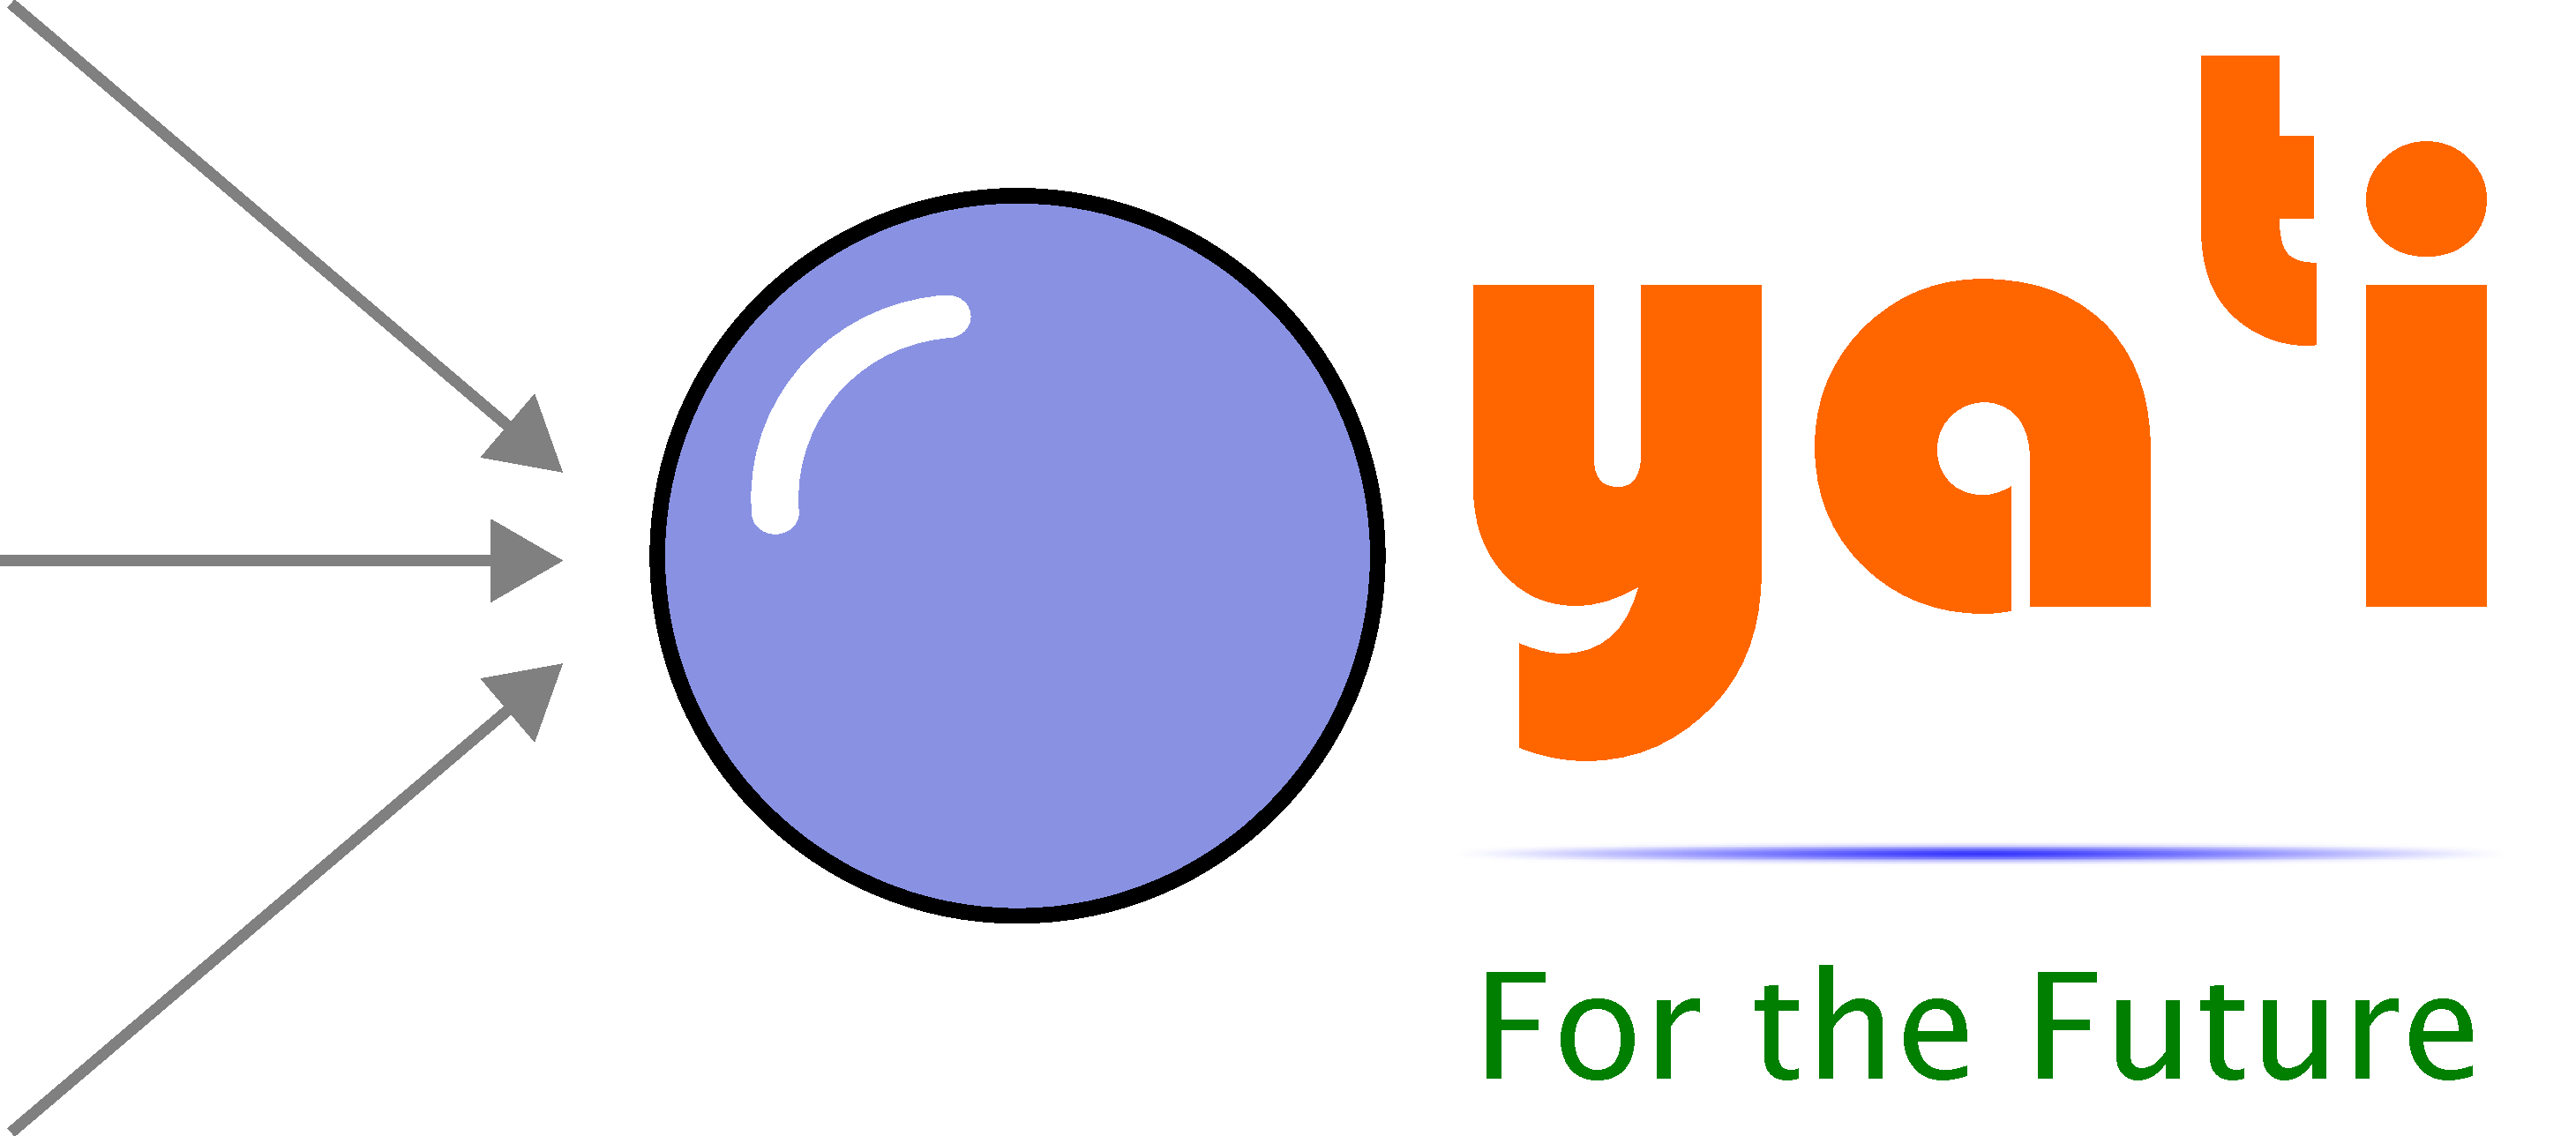
\includegraphics[width=2cm,keepaspectratio]{images/yati_logo.pdf}}
\author[Yogesh H Kulkarni]{Yogesh Kulkarni} 

\newcommand{\code}[1]{\par\vskip0pt plus 1filll \footnotesize Code:~\itshape#1}

\setbeameroption{hide notes}
\graphicspath{{./images/}}
% 
\newtheorem{axiom}{Axiom}[theorem]
%\newtheorem{conj}{Conjecture}[theorem]


%%%%
%%%% colors
%%%%
\newcommand{\TealBlue}[1]{\textcolor{TealBlue}{#1}}
\newcommand{\Peach}[1]{\textcolor{Peach}{#1}}
\newcommand{\Cyan}[1]{\textcolor{cyan}{#1}}
\newcommand{\Red}[1]{\textcolor{red}{#1}}
\newcommand{\BrickRed}[1]{\textcolor{BrickRed}{#1}}
\newcommand{\Blue}[1]{\textcolor{blue}{#1}}
\newcommand{\Green}[1]{\textcolor{green}{#1}}
\newcommand{\Black}[1]{\textcolor{black}{#1}}
\newcommand{\White}[1]{\textcolor{white}{#1}}
\newcommand{\Blueit}[1]{\textcolor{Blue}{\emph{#1}}}
\newcommand{\Magentait}[1]{\textcolor{Magenta}{\emph{#1}}}
\newcommand{\Orangeit}[1]{\textcolor{Orange}{\emph{#1}}}
\newcommand{\Greenit}[1]{\textcolor{Green}{\emph{#1}}}
\newcommand{\Cyanit}[1]{\textcolor{cyan}{\emph{#1}}}


%
%  Macros
%

\newcommand{\RingNat}{{{\mathbb{N}}}}
\newcommand{\RingInt}{{{\mathbb{Z}}}}
\newcommand{\RingReal}{{{\mathbb{R}}}}
\newcommand{\RingRat}{{{\mathbb{Q}}}}
\newcommand{\RingPosInt}{{{\mathbb{Z^+}}}}
\newcommand{\myand}{\wedge}
\newcommand{\myor}{\vee}
\newcommand{\mynot}{\neg}

% \newcommand{\pict}[3]{\resizebox{#1in}{#2in}{\includegraphics{#3}}}
\newcommand{\pictt}[1]{\includegraphics{#1}}
\newcommand{\Frac}[2]{\frac{\textstyle #1}{\textstyle #2}}

\newcommand{\der}{\operatorname{Der}} 
\newcommand{\embdim}{\operatorname{emb. dim.}} 
\newcommand{\support}{\operatorname{Support}} 
\newcommand{\coker}{\operatorname{coker}} 
\newcommand{\nind}{\noindent}
\newcommand{\Z}{\mathfrak{Z}} 
\newcommand{\E}{\mathcal{E}} 
\newcommand{\disp}{\displaystyle}

\def\bbd#1{\leavevmode\setbox0=\hbox{#1}%
   	\kern-.025em\copy0 \kern-\wd0
   	\kern .05em\copy0 \kern-\wd0
  	\kern-.025em\raise.0433em\box0
  	}
   	\def\nexto{\kern -0.54em}
    	\def\DN{ \mbox{\rm {I\ \nexto N}} }
    	\def\DZ{ \mbox{\rm Z \kern -0.82em Z} }
    	\def\DC{ \mbox{\rm\hbox{C \kern-0.8em\raise0.2ex
    	\hbox{\vrule height5.4pt width0.7pt} \kern0.45em}} }
    	\def\DQ{ \mbox{\rm\hbox{Q \kern-0.85em\raise0.25ex
    	\hbox{\vrule height5.4pt width0.7pt} \kern0.45em}} }
    	\def\DP{ \mbox{\rm\hbox{P\kern-0.75em	
    	\hbox{\vrule height9pt width0.7pt} \kern0.45em}} }
\newcommand{\bigfrac}[2]{\frac{\textstyle #1}{\textstyle #2}}
 \newcommand{\starttest}{\begin{enumerate}}
 \newcommand{\nextpage}{\vspace*{\fill}\newpage}

 \newcommand{\mat}[2]{\left( \begin{array}{*{#1}{c}}#2\end{array}\right)}
 \newcommand{\matr}[2]{\left( \begin{array}{*{#1}{r}}#2\end{array}\right)}
 
 \newcommand{\bmat}[2]{\left[ \begin{array}{*{#1}{c}}#2\end{array}\right]}
 \newcommand{\bmatr}[2]{\left[ \begin{array}{*{#1}{r}}#2\end{array}\right]}
 
 \newcommand{\dat}[2]{\left| \begin{array}{*{#1}{c}}#2\end{array}\right|}
 \newcommand{\datr}[2]{\left| \begin{array}{*{#1}{r}}#2\end{array}\right|}
 \newcommand{\deff}[1]{\vspace*{0.2in} {\bf Definition: #1}}
 \newcommand{\lineend}{\vspace*{0.1in}\centerline{\rule{4in}{0.01in}}}

 \newcommand{\seg}[1]{\overline{#1}}
 \newcommand{\ray}[1]{\overrightarrow{#1}}
 \newcommand{\lin}[1]{\overleftrightarrow{#1}}
 \newcommand{\sdash}{\!\!-\!\!}
 \newcommand{\betw}[3]{#1\sdash#2\sdash#3}
   \newcommand{\bs}{$\backslash$}

 \newcommand{\mrd}[1]{\textcolor{red}{#1}}%% Make entry red
 \newcommand{\mbl}[1]{\textcolor{blue}{#1}}%% Make entry blue
 
 \newcommand{\mgr}[1]{\textcolor{green!40!black}{#1}}%% Make entry green

\newcommand{\mbr}[1]{\textcolor{blue!55!red}{#1}}%% Make entry purple


\newtheorem{thm}{Theorem}[section]
%\newtheorem{Conjecture}[thm]{Conjecture}
%\newtheorem{Lemma}[thm]{Lemma}
%\newtheorem{corollary}[thm]{Corollary}
%\newtheorem{proposition}[thm]{Proposition} 
\newtheorem{question}[thm]{Question} 

\newtheorem*{defn}{Definition}

% \newcommand{\ignore}[1]{}
\newcommand{\arcosh}{\qopname \relax o{arcosh}}
\newcommand{\divop}{\qopname \relax o{div}}
\newcommand{\dist}{\qopname \relax o{dist}}
\newcommand{\D}{\qopname \relax o{D}\!} 	% Jacobi-Matrix
\newcommand{\dop}{\qopname \relax o{d}\!} 	% Differentialoperator
\newcommand{\ds}{\dop s}
\newcommand{\dt}{\dop t}
\newcommand{\dx}{\dop x}
\newcommand{\dy}{\dop y}
\newcommand{\Epi}{\qopname \relax o{Epi}}
\newcommand{\hot}{\qopname \relax o{hot}}
\newcommand{\id}{\qopname \relax o{id}}
\newcommand{\im}{\qopname \relax o{im}}
\newcommand{\osc}{\qopname \relax o{osc}}
%\newcommand{\rg}{\qopname \relax o{rg}}
\newcommand{\rot}{\qopname \relax o{rot}}
%\newcommand{\Satz}{Proposition }
\newcommand{\SatzEnde}{r}
\newcommand{\sgn}{\qopname \relax o{sgn}}
\newcommand{\tr}{\qopname \relax o{tr}}
\hyphenation{Hil-bert-raum}
%adrian
\newcommand{\Norm}[1]{\left\| #1 \right\|}
\newcommand{\SKP}[1]{\left\langle #1 \right\rangle}

%\newcommand\mat[2][c]{\left(\hspace{-2mm}\begin{array}{#1}#2\end{array}\hspace{-2mm}\right)}

% praktische Extras:
% Liste mit a), b) etc. vor den Items (alphanumerisch)
% zuerst der Anfang
\newcommand{\bal}[1]{\newcounter{#1}\stepcounter{#1}\begin{list}{\alph{#1})}{}}
  % jetzt die einzelnen items
  \newcommand{\aitem}[1]{\item\stepcounter{#1}}
  % zuletzt das Ende
  \newcommand{\eal}{\end{list}}
% Liste mit i), ii) etc. vor den Items (roman)
% Anfang
\newcommand{\brl}[1]{\newcounter{#1}\stepcounter{#1}\begin{list}{\roman{#1})}{}}
  % item
  \newcommand{\ritem}[1]{\item\stepcounter{#1}}
  % Ende
  \newcommand{\erl}{\end{list}}
% Matrix-Anfang und -Ende
% Anfang
\newcommand{\matb}[1]{\left(\begin{array}{#1}}
    % Ende
    \newcommand{\mate}{\end{array}\right)}
% Vektor-Anfang und -Ende
% Anfang
\newcommand{\vekb}{\left(\begin{array}{c}}
    % Ende
    \newcommand{\veke}{\end{array}\right)}
% Die Standardk�rper Q,R,C,F,N,Z
% Q
\newcommand{\Ku}{\mathbb{Q}}
% R
\newcommand{\Er}{\mathbb{R}}
% C
\newcommand{\Ze}{\mathbb{C}}
% F
\newcommand{\Ef}{\mathbb{F}}
% N
\newcommand{\En}{\mathbb{N}}
% Z
\newcommand{\Zett}{\mathbb{Z}}
% eqnarray
% Anfang
\newcommand{\bea}{\begin{eqnarray*}}
% Ende
\newcommand{\eea}{\end{eqnarray*}}
% Theoreme, S�tze, Beispiele etc.
\theoremstyle{plain}
%\newtheorem{theorem}{Theorem}[section]
%\newtheorem{korollar}[theorem]{Korollar}
%\newtheorem{lemma}[theorem]{Lemma}
\newtheorem{proposition}[theorem]{\Satz}
%\newtheorem{conjecture}[theorem]{Vermutung}
%\newtheorem{satz}[theorem]{\Satz}
%\theoremstyle{definition}
%\newtheorem{definition}[theorem]{Definition}
%%\theoremstyle{remark}
%\newtheorem{notation}[theorem]{Notation}
%\newtheorem{remark}[theorem]{Remark}
%\newtheorem{corollary}[theorem]{Corollary}
%\newtheorem{application}[theorem]{Application}
%\newtheorem{example}[theorem]{Example}
%\newtheorem*{remark*}{Bemerkung}
%\newtheorem*{example*}{Example}
%\newtheorem*{notation*}{Bezeichnung}
%\newtheorem*{application*}{Anwendung}

%\newenvironment{proof}[1][Beweis]{\begin{trivlist}
%  \item[\hskip \labelsep {\bfseries #1}]}{\end{trivlist}}
% \newenvironment{definition}[1][Definition]{\begin{trivlist}
% \item[\hskip \labelsep {\bfseries #1}]}{\end{trivlist}}
%\newenvironment{example}[1][Example]{\begin{trivlist}
%  \item[\hskip \labelsep {\bfseries #1}]}{\end{trivlist}}
%\newenvironment{remark}[1][Remark]{\begin{trivlist}
%  \item[\hskip \labelsep {\bfseries #1}]}{\end{trivlist}}

% Beginn Symboldef Mitterlwertintegral-----------------------------------
\def \Xint #1{\mathchoice						
  {\XXint \displaystyle \textstyle {#1}} %
  {\XXint \textstyle \scriptstyle {#1}} %
  {\XXint \scriptstyle \scriptscriptstyle {#1}} %
  {\XXint \scriptscriptstyle \scriptscriptstyle {#1}} %
  \!\int }

\def \XXint #1#2#3{{\setbox 0=\hbox {$#1{#2#3}{\int }$}\vcenter {\hbox {$#2#3$}}\kern -0.5\wd 0}}

\def \dashint {\Xint -}							

% Fallunterscheidung
\newcommand {\Fall}[5]
    { #1 = \left \{
        \begin{array}
         {c@ {\quad \mbox{ if } \quad} l}
          #2 & #3 \\
           #4 & #5           \end{array}
            \right .    }


\newcommand {\Falldrei}[7]
       { #1 = \left \{
          \begin{array}
             {c@ {\quad \mbox{ if } \quad} l}
               #2 & #3 \\
            #4 & #5 \\ 														             \right .    }



% \renewcommand{\P}{\text{P}}
%\newcommand{\R}{{\rm I\!R}}
\newcommand{\pr}{{\rm I\!P}}
%%%\newcommand{\E}{{\rm I\!E}}
\newcommand{\Na}{{\rm I\!N}}
\newtheorem{conj}{Conjecture}
\newtheorem{countex}{Counterexample}
\newtheorem{prop}{Proposition}
%%%\newtheorem{thm}{Theorem}
\newtheorem{cor}{Corollary}
%%%\newtheorem{defn}{Definition}
\newtheorem{lem}{Lemma}
%\renewcommand{\ell}{l}
\newcommand{\SSS}{\scriptscriptstyle}
\newcommand{\MC}{\multicolumn}
\newcommand{\cT}{\ensuremath{{\cal T}}}
\newcommand{\z}{\ensuremath{\pi}}
\newcommand{\sZ}{\ensuremath{\Pi}}
\newcommand{\bz}{\ensuremath{\mbox{\boldmath$\pi$}}}
\newcommand{\Pperm}{\ensuremath{{\hat{P}}}}
\newcommand{\Pnull}{\ensuremath{{{P}_{\mbox{null}}}}}
\newcommand{\bx}{\ensuremath{{\bf x}}}
\newcommand{\bzz}{\ensuremath{{\bf z}}}
\def\ssucc{{\succ\!\!\!\!\succ}}
%\DeclareMathOperator\Tr{Tr}
% set up hyperlink colors
\hypersetup{colorlinks=true,anchorcolor=green,linkcolor=red,menucolor=cyan}
%%================Math symbol ============================
\def\nn{{\mathbb N}}
\def\zz{{\mathbb Z}}
\def\rr{{\mathbb R}}
\def\rn{{\mathbb R}^n}
\def\ym{Y^{m}}\def\xm{X^{m}}
\def\yp{Y^{p}}\def\xp{X^{p}}
\def\yr{Y^{r}}\def\xr{X^{r}}
\def\yj{Y^{j}}\def\xj{X^{j}}

\def\yij#1#2{y_{#2}^{#1}}\def\xij#1#2{x_{#2}^{#1}}


%%=============Display style operator =====================
\def\dsum{\displaystyle\sum}
\def\dint{\displaystyle\int}
\def\dfrac{\displaystyle\frac}
\def\dsup{\displaystyle\sup}
\def\dinf{\displaystyle\inf}
\def\dmin{\displaystyle\min}
\def\dlim{\displaystyle\lim}


%%=========Greek Letters =================
\def\gep{\varepsilon}
\def\ga{\alpha}
\def\gb{\beta}
\def\gs{\sigma}
\def\gd{\delta}
\def\gl{\lambda}
\def\gga{\gamma}
\def\gS{\Sigma}
\def\gD{\Delta}
\def\px{{\rho\!_{_X}}}
\def\L{{\cal L}} %
\def\B{{\cal B}} %
\def\X{{\cal X}} %
\def\M{{\cal M}} %

%============ Special notations ===============
\newcommand{\set}[1]{\left\{#1\right\}} % set
\def\E{{\mathcal E}} % generalization error
\def\H{{\mathcal H}} % hypothesis space
\def\H{{\mathcal H}} % hypothesis space
\def\N{{\mathcal N}} % covering number
\def\D{{\mathcal D}} % regularization error
\def\bz{{\bf z}} % sample
%%%\DeclareMathOperator\sgn{sgn} % sign function
\DeclareMathOperator\Span{span} % linear span
\DeclareMathOperator\Diam{Diam} % diameter of a set
\DeclareMathOperator\bE{\mathbb E} % expectation
\DeclareMathOperator*\prob{{\bf P}rob} % probability in product space


% %\makeatletter
\DeclareRobustCommand*{\savepause}[1]{\only<1>{\immediate\write\@auxout{\string\pauseentry{\the\c@framenumber}{#1}{\the\c@beamerpauses}}}}
\newcommand*{\usepause}[1]{\@ifundefined{pauses@\the\c@framenumber @#1}{1}{\@nameuse{pauses@\the\c@framenumber @#1}}}
\newcommand*{\pauseentry}[3]{\global\@namedef{pauses@#1@#2}{#3}}

\makeatother\newcommand{\floor}[1]{\lfloor{#1}\rfloor}

\setbeamertemplate{navigation symbols}{}
\tikzset{
vertex/.style={circle,draw=blue!50,thick},
}
\tikzset{
vertex/.style={circle,draw=blue!50,thick},
}

\tikzset{
bluedot/.style={circle,draw=blue,fill=blue,thick},
}

\tikzset{
littlevertx/.style={minimum width=1pt,minimum width=1pt,text width=1pt},
}



\tikzset{
dot/.style={circle,draw=black,thick},
}

\tikzset{
reddot/.style={circle,draw=red,fill=red,thick},
}

\tikzset{
orangedot/.style={circle,draw=orange,fill=orange ,thick},
}

\tikzset{
packet/.style={rectangle,draw=black,fill=white,thick},
}

\tikzset{
lostpacket/.style={rectangle,draw=red,fill=red,thick},
}

\tikzset{
corruptpacket/.style={rectangle,draw=red,thick},
}

\tikzset{
greendot/.style={circle,draw=green,fill=green,thick},
}

\tikzset{
entity/.style={rectangle,draw=blue!50,thick},
}
\newcommand{\bl}[2]{{\color<#1>{blue} #2}}
\renewcommand{\gl}[2]{{\color<#1>{green} #2}}
\newcommand{\rl}[2]{{\color<#1>{red} #2}}
\newcommand{\orl}[2]{{\color<#1>{orange} #2}}
\newcommand{\ol}[2]{{\onslide<#1>{#2}}}
\newcommand{\xor}{\oplus}

\newcommand{\spd}[1]{#1 {\color{black} \spadesuit}}
\newcommand{\clb}[1]{#1 {\color{black} \clubsuit}}
\newcommand{\dmd}[1]{#1 {\color{red} \diamondsuit}}
\newcommand{\hrt}[1]{#1 {\color{red} \heartsuit}}

\newcommand{\hl}[1]{{\color{blue}#1}}
\newcommand{\orli}[1]{{\color{orange}#1}}
%\usepackage{pstricks, pst-node}

%
%	THE GRID - UNLABELED VERTICES
%
\newcommand{\Gaa}{\put(0,0){\circle*{3}}}
\newcommand{\Gba}{\put(10,0){\circle*{3}}}
\newcommand{\Gca}{\put(20,0){\circle*{3}}}
\newcommand{\Gda}{\put(30,0){\circle*{3}}}
\newcommand{\Gea}{\put(40,0){\circle*{3}}}
\newcommand{\Gfa}{\put(50,0){\circle*{3}}}
\newcommand{\Gga}{\put(60,0){\circle*{3}}}

\newcommand{\Gab}{\put(0,10){\circle*{3}}}
\newcommand{\Gbb}{\put(10,10){\circle*{3}}}
\newcommand{\Gcb}{\put(20,10){\circle*{3}}}
\newcommand{\Gdb}{\put(30,10){\circle*{3}}}
\newcommand{\Geb}{\put(40,10){\circle*{3}}}
\newcommand{\Gfb}{\put(50,10){\circle*{3}}}
\newcommand{\Ggb}{\put(60,10){\circle*{3}}}

\newcommand{\Gac}{\put(0,20){\circle*{3}}}
\newcommand{\Gbc}{\put(10,20){\circle*{3}}}
\newcommand{\Gcc}{\put(20,20){\circle*{3}}}
\newcommand{\Gdc}{\put(30,20){\circle*{3}}}
\newcommand{\Gec}{\put(40,20){\circle*{3}}}
\newcommand{\Gfc}{\put(50,20){\circle*{3}}}
\newcommand{\Ggc}{\put(60,20){\circle*{3}}}

\newcommand{\Gad}{\put(0,30){\circle*{3}}}
\newcommand{\Gbd}{\put(10,30){\circle*{3}}}
\newcommand{\Gcd}{\put(20,30){\circle*{3}}}
\newcommand{\Gdd}{\put(30,30){\circle*{3}}}
\newcommand{\Ged}{\put(40,30){\circle*{3}}}
\newcommand{\Gfd}{\put(50,30){\circle*{3}}}
\newcommand{\Ggd}{\put(60,30){\circle*{3}}}

\newcommand{\Gae}{\put(0,40){\circle*{3}}}
\newcommand{\Gbe}{\put(10,40){\circle*{3}}}
\newcommand{\Gce}{\put(20,40){\circle*{3}}}
\newcommand{\Gde}{\put(30,40){\circle*{3}}}
\newcommand{\Gee}{\put(40,40){\circle*{3}}}
\newcommand{\Gfe}{\put(50,40){\circle*{3}}}
\newcommand{\Gge}{\put(60,40){\circle*{3}}}

\newcommand{\Gaf}{\put(0,50){\circle*{3}}}
\newcommand{\Gbf}{\put(10,50){\circle*{3}}}
\newcommand{\Gcf}{\put(20,50){\circle*{3}}}
\newcommand{\Gdf}{\put(30,50){\circle*{3}}}
\newcommand{\Gef}{\put(40,50){\circle*{3}}}
\newcommand{\Gff}{\put(50,50){\circle*{3}}}
\newcommand{\Ggf}{\put(60,50){\circle*{3}}}

\newcommand{\Gag}{\put(0,60){\circle*{3}}}
\newcommand{\Gbg}{\put(10,60){\circle*{3}}}
\newcommand{\Gcg}{\put(20,60){\circle*{3}}}
\newcommand{\Gdg}{\put(30,60){\circle*{3}}}
\newcommand{\Geg}{\put(40,60){\circle*{3}}}
\newcommand{\Gfg}{\put(50,60){\circle*{3}}}
\newcommand{\Ggg}{\put(60,60){\circle*{3}}}

%
%	THE GRID - UNLABELED VERTICES, VARIABLE SIZE
%
\newcommand{\GaaV}[1]{\put(0,0){\circle*{#1}}}
\newcommand{\GbaV}[1]{\put(10,0){\circle*{#1}}}
\newcommand{\GcaV}[1]{\put(20,0){\circle*{#1}}}
\newcommand{\GdaV}[1]{\put(30,0){\circle*{#1}}}
\newcommand{\GeaV}[1]{\put(40,0){\circle*{#1}}}
\newcommand{\GfaV}[1]{\put(50,0){\circle*{#1}}}
\newcommand{\GgaV}[1]{\put(60,0){\circle*{#1}}}

\newcommand{\GabV}[1]{\put(0,10){\circle*{#1}}}
\newcommand{\GbbV}[1]{\put(10,10){\circle*{#1}}}
\newcommand{\GcbV}[1]{\put(20,10){\circle*{#1}}}
\newcommand{\GdbV}[1]{\put(30,10){\circle*{#1}}}
\newcommand{\GebV}[1]{\put(40,10){\circle*{#1}}}
\newcommand{\GfbV}[1]{\put(50,10){\circle*{#1}}}
\newcommand{\GgbV}[1]{\put(60,10){\circle*{#1}}}

\newcommand{\GacV}[1]{\put(0,20){\circle*{#1}}}
\newcommand{\GbcV}[1]{\put(10,20){\circle*{#1}}}
\newcommand{\GccV}[1]{\put(20,20){\circle*{#1}}}
\newcommand{\GdcV}[1]{\put(30,20){\circle*{#1}}}
\newcommand{\GecV}[1]{\put(40,20){\circle*{#1}}}
\newcommand{\GfcV}[1]{\put(50,20){\circle*{#1}}}
\newcommand{\GgcV}[1]{\put(60,20){\circle*{#1}}}

\newcommand{\GadV}[1]{\put(0,30){\circle*{#1}}}
\newcommand{\GbdV}[1]{\put(10,30){\circle*{#1}}}
\newcommand{\GcdV}[1]{\put(20,30){\circle*{#1}}}
\newcommand{\GddV}[1]{\put(30,30){\circle*{#1}}}
\newcommand{\GedV}[1]{\put(40,30){\circle*{#1}}}
\newcommand{\GfdV}[1]{\put(50,30){\circle*{#1}}}
\newcommand{\GgdV}[1]{\put(60,30){\circle*{#1}}}

\newcommand{\GaeV}[1]{\put(0,40){\circle*{#1}}}
\newcommand{\GbeV}[1]{\put(10,40){\circle*{#1}}}
\newcommand{\GceV}[1]{\put(20,40){\circle*{#1}}}
\newcommand{\GdeV}[1]{\put(30,40){\circle*{#1}}}
\newcommand{\GeeV}[1]{\put(40,40){\circle*{#1}}}
\newcommand{\GfeV}[1]{\put(50,40){\circle*{#1}}}
\newcommand{\GgeV}[1]{\put(60,40){\circle*{#1}}}

\newcommand{\GafV}[1]{\put(0,50){\circle*{#1}}}
\newcommand{\GbfV}[1]{\put(10,50){\circle*{#1}}}
\newcommand{\GcfV}[1]{\put(20,50){\circle*{#1}}}
\newcommand{\GdfV}[1]{\put(30,50){\circle*{#1}}}
\newcommand{\GefV}[1]{\put(40,50){\circle*{#1}}}
\newcommand{\GffV}[1]{\put(50,50){\circle*{#1}}}
\newcommand{\GgfV}[1]{\put(60,50){\circle*{#1}}}

\newcommand{\GagV}[1]{\put(0,60){\circle*{#1}}}
\newcommand{\GbgV}[1]{\put(10,60){\circle*{#1}}}
\newcommand{\GcgV}[1]{\put(20,60){\circle*{#1}}}
\newcommand{\GdgV}[1]{\put(30,60){\circle*{#1}}}
\newcommand{\GegV}[1]{\put(40,60){\circle*{#1}}}
\newcommand{\GfgV}[1]{\put(50,60){\circle*{#1}}}
\newcommand{\GggV}[1]{\put(60,60){\circle*{#1}}}


%
%	THE GRID - LABLED VERTICES
%	

\newcommand{\GaaL}[2]{\Gaa \put(0,0){\makebox(0,0){\hspace{#1}#2}}}
\newcommand{\GbaL}[2]{\Gba \put(10,0){\makebox(0,0){\hspace{#1}#2}}}
\newcommand{\GcaL}[2]{\Gca \put(20,0){\makebox(0,0){\hspace{#1}#2}}}
\newcommand{\GdaL}[2]{\Gda \put(30,0){\makebox(0,0){\hspace{#1}#2}}}
\newcommand{\GeaL}[2]{\Gea \put(40,0){\makebox(0,0){\hspace{#1}#2}}}
\newcommand{\GfaL}[2]{\Gfa \put(50,0){\makebox(0,0){\hspace{#1}#2}}}
\newcommand{\GgaL}[2]{\Gga \put(60,0){\makebox(0,0){\hspace{#1}#2}}}

\newcommand{\GabL}[2]{\Gab \put(0,10){\makebox(0,0){\hspace{#1}#2}}}
\newcommand{\GbbL}[2]{\Gbb \put(10,10){\makebox(0,0){\hspace{#1}#2}}}
\newcommand{\GcbL}[2]{\Gcb \put(20,10){\makebox(0,0){\hspace{#1}#2}}}
\newcommand{\GdbL}[2]{\Gdb \put(30,10){\makebox(0,0){\hspace{#1}#2}}}
\newcommand{\GebL}[2]{\Geb \put(40,10){\makebox(0,0){\hspace{#1}#2}}}
\newcommand{\GfbL}[2]{\Gfb \put(50,10){\makebox(0,0){\hspace{#1}#2}}}
\newcommand{\GgbL}[2]{\Ggb \put(60,10){\makebox(0,0){\hspace{#1}#2}}}

\newcommand{\GacL}[2]{\Gac \put(0,20){\makebox(0,0){\hspace{#1}#2}}}
\newcommand{\GbcL}[2]{\Gbc \put(10,20){\makebox(0,0){\hspace{#1}#2}}}
\newcommand{\GccL}[2]{\Gcc \put(20,20){\makebox(0,0){\hspace{#1}#2}}}
\newcommand{\GdcL}[2]{\Gdc \put(30,20){\makebox(0,0){\hspace{#1}#2}}}
\newcommand{\GecL}[2]{\Gec \put(40,20){\makebox(0,0){\hspace{#1}#2}}}
\newcommand{\GfcL}[2]{\Gfc \put(50,20){\makebox(0,0){\hspace{#1}#2}}}
\newcommand{\GgcL}[2]{\Ggc \put(60,20){\makebox(0,0){\hspace{#1}#2}}}

\newcommand{\GadL}[2]{\Gad \put(0,30){\makebox(0,0){\hspace{#1}#2}}}
\newcommand{\GbdL}[2]{\Gbd \put(10,30){\makebox(0,0){\hspace{#1}#2}}}
\newcommand{\GcdL}[2]{\Gcd \put(20,30){\makebox(0,0){\hspace{#1}#2}}}
\newcommand{\GddL}[2]{\Gdd \put(30,30){\makebox(0,0){\hspace{#1}#2}}}
\newcommand{\GedL}[2]{\Ged \put(40,30){\makebox(0,0){\hspace{#1}#2}}}
\newcommand{\GfdL}[2]{\Gfd \put(50,30){\makebox(0,0){\hspace{#1}#2}}}
\newcommand{\GgdL}[2]{\Ggd \put(60,30){\makebox(0,0){\hspace{#1}#2}}}

\newcommand{\GaeL}[2]{\Gae \put(0,40){\makebox(0,0){\hspace{#1}#2}}}
\newcommand{\GbeL}[2]{\Gbe \put(10,40){\makebox(0,0){\hspace{#1}#2}}}
\newcommand{\GceL}[2]{\Gce \put(20,40){\makebox(0,0){\hspace{#1}#2}}}
\newcommand{\GdeL}[2]{\Gde \put(30,40){\makebox(0,0){\hspace{#1}#2}}}
\newcommand{\GeeL}[2]{\Gee \put(40,40){\makebox(0,0){\hspace{#1}#2}}}
\newcommand{\GfeL}[2]{\Gfe \put(50,40){\makebox(0,0){\hspace{#1}#2}}}
\newcommand{\GgeL}[2]{\Gge \put(60,40){\makebox(0,0){\hspace{#1}#2}}}

\newcommand{\GafL}[2]{\Gaf \put(0,50){\makebox(0,0){\hspace{#1}#2}}}
\newcommand{\GbfL}[2]{\Gbf \put(10,50){\makebox(0,0){\hspace{#1}#2}}}
\newcommand{\GcfL}[2]{\Gcf \put(20,50){\makebox(0,0){\hspace{#1}#2}}}
\newcommand{\GdfL}[2]{\Gdf \put(30,50){\makebox(0,0){\hspace{#1}#2}}}
\newcommand{\GefL}[2]{\Gef \put(40,50){\makebox(0,0){\hspace{#1}#2}}}
\newcommand{\GffL}[2]{\Gff \put(50,50){\makebox(0,0){\hspace{#1}#2}}}
\newcommand{\GgfL}[2]{\Ggf \put(60,50){\makebox(0,0){\hspace{#1}#2}}}

\newcommand{\GagL}[2]{\Gag \put(0,60){\makebox(0,0){\hspace{#1}#2}}}
\newcommand{\GbgL}[2]{\Gbg \put(10,60){\makebox(0,0){\hspace{#1}#2}}}
\newcommand{\GcgL}[2]{\Gcg \put(20,60){\makebox(0,0){\hspace{#1}#2}}}
\newcommand{\GdgL}[2]{\Gdg \put(30,60){\makebox(0,0){\hspace{#1}#2}}}
\newcommand{\GegL}[2]{\Geg \put(40,60){\makebox(0,0){\hspace{#1}#2}}}
\newcommand{\GfgL}[2]{\Gfg \put(50,60){\makebox(0,0){\hspace{#1}#2}}}
\newcommand{\GggL}[2]{\Ggg \put(60,60){\makebox(0,0){\hspace{#1}#2}}}

%
%	THE GRID - LABLED VERTICES, VARIABLE SIZE
%	

\newcommand{\GaaLV}[3]{\GaaV{#3} \put(0,0){\makebox(0,0){\hspace{#1}#2}}}
\newcommand{\GbaLV}[3]{\GbaV{#3} \put(10,0){\makebox(0,0){\hspace{#1}#2}}}
\newcommand{\GcaLV}[3]{\GcaV{#3} \put(20,0){\makebox(0,0){\hspace{#1}#2}}}
\newcommand{\GdaLV}[3]{\GdaV{#3} \put(30,0){\makebox(0,0){\hspace{#1}#2}}}
\newcommand{\GeaLV}[3]{\GeaV{#3} \put(40,0){\makebox(0,0){\hspace{#1}#2}}}
\newcommand{\GfaLV}[3]{\GfaV{#3} \put(50,0){\makebox(0,0){\hspace{#1}#2}}}
\newcommand{\GgaLV}[3]{\GgaV{#3} \put(60,0){\makebox(0,0){\hspace{#1}#2}}}

\newcommand{\GabLV}[3]{\GabV{#3} \put(0,10){\makebox(0,0){\hspace{#1}#2}}}
\newcommand{\GbbLV}[3]{\GbbV{#3} \put(10,10){\makebox(0,0){\hspace{#1}#2}}}
\newcommand{\GcbLV}[3]{\GcbV{#3} \put(20,10){\makebox(0,0){\hspace{#1}#2}}}
\newcommand{\GdbLV}[3]{\GdbV{#3} \put(30,10){\makebox(0,0){\hspace{#1}#2}}}
\newcommand{\GebLV}[3]{\GebV{#3} \put(40,10){\makebox(0,0){\hspace{#1}#2}}}
\newcommand{\GfbLV}[3]{\GfbV{#3} \put(50,10){\makebox(0,0){\hspace{#1}#2}}}
\newcommand{\GgbLV}[3]{\GgbV{#3} \put(60,10){\makebox(0,0){\hspace{#1}#2}}}

\newcommand{\GacLV}[3]{\GacV{#3} \put(0,20){\makebox(0,0){\hspace{#1}#2}}}
\newcommand{\GbcLV}[3]{\GbcV{#3} \put(10,20){\makebox(0,0){\hspace{#1}#2}}}
\newcommand{\GccLV}[3]{\GccV{#3} \put(20,20){\makebox(0,0){\hspace{#1}#2}}}
\newcommand{\GdcLV}[3]{\GdcV{#3} \put(30,20){\makebox(0,0){\hspace{#1}#2}}}
\newcommand{\GecLV}[3]{\GecV{#3} \put(40,20){\makebox(0,0){\hspace{#1}#2}}}
\newcommand{\GfcLV}[3]{\GfcV{#3} \put(50,20){\makebox(0,0){\hspace{#1}#2}}}
\newcommand{\GgcLV}[3]{\GgcV{#3} \put(60,20){\makebox(0,0){\hspace{#1}#2}}}

\newcommand{\GadLV}[3]{\GadV{#3} \put(0,30){\makebox(0,0){\hspace{#1}#2}}}
\newcommand{\GbdLV}[3]{\GbdV{#3} \put(10,30){\makebox(0,0){\hspace{#1}#2}}}
\newcommand{\GcdLV}[3]{\GcdV{#3} \put(20,30){\makebox(0,0){\hspace{#1}#2}}}
\newcommand{\GddLV}[3]{\GddV{#3} \put(30,30){\makebox(0,0){\hspace{#1}#2}}}
\newcommand{\GedLV}[3]{\GedV{#3} \put(40,30){\makebox(0,0){\hspace{#1}#2}}}
\newcommand{\GfdLV}[3]{\GfdV{#3} \put(50,30){\makebox(0,0){\hspace{#1}#2}}}
\newcommand{\GgdLV}[3]{\GgdV{#3} \put(60,30){\makebox(0,0){\hspace{#1}#2}}}

\newcommand{\GaeLV}[3]{\GaeV{#3} \put(0,40){\makebox(0,0){\hspace{#1}#2}}}
\newcommand{\GbeLV}[3]{\GbeV{#3} \put(10,40){\makebox(0,0){\hspace{#1}#2}}}
\newcommand{\GceLV}[3]{\GceV{#3} \put(20,40){\makebox(0,0){\hspace{#1}#2}}}
\newcommand{\GdeLV}[3]{\GdeV{#3} \put(30,40){\makebox(0,0){\hspace{#1}#2}}}
\newcommand{\GeeLV}[3]{\GeeV{#3} \put(40,40){\makebox(0,0){\hspace{#1}#2}}}
\newcommand{\GfeLV}[3]{\GfeV{#3} \put(50,40){\makebox(0,0){\hspace{#1}#2}}}
\newcommand{\GgeLV}[3]{\GgeV{#3} \put(60,40){\makebox(0,0){\hspace{#1}#2}}}

\newcommand{\GafLV}[3]{\GafV{#3} \put(0,50){\makebox(0,0){\hspace{#1}#2}}}
\newcommand{\GbfLV}[3]{\GbfV{#3} \put(10,50){\makebox(0,0){\hspace{#1}#2}}}
\newcommand{\GcfLV}[3]{\GcfV{#3} \put(20,50){\makebox(0,0){\hspace{#1}#2}}}
\newcommand{\GdfLV}[3]{\GdfV{#3} \put(30,50){\makebox(0,0){\hspace{#1}#2}}}
\newcommand{\GefLV}[3]{\GefV{#3} \put(40,50){\makebox(0,0){\hspace{#1}#2}}}
\newcommand{\GffLV}[3]{\GffV{#3} \put(50,50){\makebox(0,0){\hspace{#1}#2}}}
\newcommand{\GgfLV}[3]{\GgfV{#3} \put(60,50){\makebox(0,0){\hspace{#1}#2}}}

\newcommand{\GagLV}[3]{\GagV{#3} \put(0,60){\makebox(0,0){\hspace{#1}#2}}}
\newcommand{\GbgLV}[3]{\GbgV{#3} \put(10,60){\makebox(0,0){\hspace{#1}#2}}}
\newcommand{\GcgLV}[3]{\GcgV{#3} \put(20,60){\makebox(0,0){\hspace{#1}#2}}}
\newcommand{\GdgLV}[3]{\GdgV{#3} \put(30,60){\makebox(0,0){\hspace{#1}#2}}}
\newcommand{\GegLV}[3]{\GegV{#3} \put(40,60){\makebox(0,0){\hspace{#1}#2}}}
\newcommand{\GfgLV}[3]{\GfgV{#3} \put(50,60){\makebox(0,0){\hspace{#1}#2}}}
\newcommand{\GggLV}[3]{\GggV{#3} \put(60,60){\makebox(0,0){\hspace{#1}#2}}}


%
%	THE GRID - UNLABELED EDGES
%
\newcommand{\Gaaba}{\put(0,0){\line(1,0){10}}}
\newcommand{\Gaaca}{\put(0,0){\line(1,0){20}}}
\newcommand{\Gaada}{\put(0,0){\line(1,0){30}}}
\newcommand{\Gaaea}{\put(0,0){\line(1,0){40}}}
\newcommand{\Gaafa}{\put(0,0){\line(1,0){50}}}
\newcommand{\Gaaga}{\put(0,0){\line(1,0){60}}}

\newcommand{\Gaaab}{\put(0,0){\line(0,1){10}}}
\newcommand{\Gaabb}{\put(0,0){\line(1,1){10}}}
\newcommand{\Gaacb}{\put(0,0){\line(2,1){20}}}
\newcommand{\Gaadb}{\put(0,0){\line(3,1){30}}}
\newcommand{\Gaaeb}{\put(0,0){\line(4,1){40}}}
\newcommand{\Gaafb}{\put(0,0){\line(5,1){50}}}
\newcommand{\Gaagb}{\put(0,0){\line(6,1){60}}}

\newcommand{\Gaaac}{\put(0,0){\line(0,1){20}}}
\newcommand{\Gaabc}{\put(0,0){\line(1,2){10}}}
\newcommand{\Gaacc}{\put(0,0){\line(1,1){20}}}
\newcommand{\Gaadc}{\put(0,0){\line(3,2){30}}}
\newcommand{\Gaaec}{\put(0,0){\line(2,1){40}}}
\newcommand{\Gaafc}{\put(0,0){\line(5,2){50}}}
\newcommand{\Gaagc}{\put(0,0){\line(3,1){60}}}

\newcommand{\Gaaad}{\put(0,0){\line(0,1){30}}}
\newcommand{\Gaabd}{\put(0,0){\line(1,3){10}}}
\newcommand{\Gaacd}{\put(0,0){\line(2,3){20}}}
\newcommand{\Gaadd}{\put(0,0){\line(1,1){30}}}
\newcommand{\Gaaed}{\put(0,0){\line(4,3){40}}}
\newcommand{\Gaafd}{\put(0,0){\line(5,3){50}}}
\newcommand{\Gaagd}{\put(0,0){\line(2,1){60}}}

\newcommand{\Gaaae}{\put(0,0){\line(0,1){40}}}
\newcommand{\Gaabe}{\put(0,0){\line(1,4){10}}}
\newcommand{\Gaace}{\put(0,0){\line(1,2){20}}}
\newcommand{\Gaade}{\put(0,0){\line(3,4){30}}}
\newcommand{\Gaaee}{\put(0,0){\line(1,1){40}}}
\newcommand{\Gaafe}{\put(0,0){\line(5,4){50}}}
\newcommand{\Gaage}{\put(0,0){\line(3,2){60}}}

\newcommand{\Gaaaf}{\put(0,0){\line(0,1){50}}}
\newcommand{\Gaabf}{\put(0,0){\line(1,5){10}}}
\newcommand{\Gaacf}{\put(0,0){\line(2,5){20}}}
\newcommand{\Gaadf}{\put(0,0){\line(3,5){30}}}
\newcommand{\Gaaef}{\put(0,0){\line(4,5){40}}}
\newcommand{\Gaaff}{\put(0,0){\line(1,1){50}}}
\newcommand{\Gaagf}{\put(0,0){\line(6,5){60}}}

\newcommand{\Gaaag}{\put(0,0){\line(0,1){60}}}
\newcommand{\Gaabg}{\put(0,0){\line(1,6){10}}}
\newcommand{\Gaacg}{\put(0,0){\line(1,3){20}}}
\newcommand{\Gaadg}{\put(0,0){\line(1,2){30}}}
\newcommand{\Gaaeg}{\put(0,0){\line(2,3){40}}}
\newcommand{\Gaafg}{\put(0,0){\line(5,6){50}}}
\newcommand{\Gaagg}{\put(0,0){\line(1,1){60}}}

%----

\newcommand{\Gbaca}{\put(10,0){\line(1,0){10}}}
\newcommand{\Gbada}{\put(10,0){\line(1,0){20}}}
\newcommand{\Gbaea}{\put(10,0){\line(1,0){30}}}
\newcommand{\Gbafa}{\put(10,0){\line(1,0){40}}}
\newcommand{\Gbaga}{\put(10,0){\line(1,0){50}}}

\newcommand{\Gbaab}{\put(10,0){\line(-1,1){10}}}
\newcommand{\Gbabb}{\put(10,0){\line(0,1){10}}}
\newcommand{\Gbacb}{\put(10,0){\line(1,1){10}}}
\newcommand{\Gbadb}{\put(10,0){\line(2,1){20}}}
\newcommand{\Gbaeb}{\put(10,0){\line(3,1){30}}}
\newcommand{\Gbafb}{\put(10,0){\line(4,1){40}}}
\newcommand{\Gbagb}{\put(10,0){\line(5,1){50}}}

\newcommand{\Gbaac}{\put(10,0){\line(-1,2){10}}}
\newcommand{\Gbabc}{\put(10,0){\line(0,1){20}}}
\newcommand{\Gbacc}{\put(10,0){\line(1,2){10}}}
\newcommand{\Gbadc}{\put(10,0){\line(1,1){20}}}
\newcommand{\Gbaec}{\put(10,0){\line(3,2){30}}}
\newcommand{\Gbafc}{\put(10,0){\line(2,1){40}}}
\newcommand{\Gbagc}{\put(10,0){\line(5,2){50}}}

\newcommand{\Gbaad}{\put(10,0){\line(-1,3){10}}}
\newcommand{\Gbabd}{\put(10,0){\line(0,1){30}}}
\newcommand{\Gbacd}{\put(10,0){\line(1,3){10}}}
\newcommand{\Gbadd}{\put(10,0){\line(2,3){20}}}
\newcommand{\Gbaed}{\put(10,0){\line(1,1){30}}}
\newcommand{\Gbafd}{\put(10,0){\line(4,3){40}}}
\newcommand{\Gbagd}{\put(10,0){\line(5,3){50}}}

\newcommand{\Gbaae}{\put(10,0){\line(-1,4){10}}}
\newcommand{\Gbabe}{\put(10,0){\line(0,1){40}}}
\newcommand{\Gbace}{\put(10,0){\line(1,4){10}}}
\newcommand{\Gbade}{\put(10,0){\line(1,2){20}}}
\newcommand{\Gbaee}{\put(10,0){\line(3,4){30}}}
\newcommand{\Gbafe}{\put(10,0){\line(1,1){40}}}
\newcommand{\Gbage}{\put(10,0){\line(5,4){50}}}

\newcommand{\Gbaaf}{\put(10,0){\line(-1,5){10}}}
\newcommand{\Gbabf}{\put(10,0){\line(0,1){50}}}
\newcommand{\Gbacf}{\put(10,0){\line(1,5){10}}}
\newcommand{\Gbadf}{\put(10,0){\line(2,5){20}}}
\newcommand{\Gbaef}{\put(10,0){\line(3,5){30}}}
\newcommand{\Gbaff}{\put(10,0){\line(4,5){40}}}
\newcommand{\Gbagf}{\put(10,0){\line(1,1){50}}}

\newcommand{\Gbaag}{\put(10,0){\line(-1,6){10}}}
\newcommand{\Gbabg}{\put(10,0){\line(0,1){60}}}
\newcommand{\Gbacg}{\put(10,0){\line(1,6){10}}}
\newcommand{\Gbadg}{\put(10,0){\line(1,3){20}}}
\newcommand{\Gbaeg}{\put(10,0){\line(1,2){30}}}
\newcommand{\Gbafg}{\put(10,0){\line(2,3){40}}}
\newcommand{\Gbagg}{\put(10,0){\line(5,6){50}}}

%----

\newcommand{\Gcada}{\put(20,0){\line(1,0){10}}}
\newcommand{\Gcaea}{\put(20,0){\line(1,0){20}}}
\newcommand{\Gcafa}{\put(20,0){\line(1,0){30}}}
\newcommand{\Gcaga}{\put(20,0){\line(1,0){40}}}

\newcommand{\Gcaab}{\put(20,0){\line(-2,1){20}}}
\newcommand{\Gcabb}{\put(20,0){\line(-1,1){10}}}
\newcommand{\Gcacb}{\put(20,0){\line(0,1){10}}}
\newcommand{\Gcadb}{\put(20,0){\line(1,1){10}}}
\newcommand{\Gcaeb}{\put(20,0){\line(2,1){20}}}
\newcommand{\Gcafb}{\put(20,0){\line(3,1){30}}}
\newcommand{\Gcagb}{\put(20,0){\line(4,1){40}}}

\newcommand{\Gcaac}{\put(20,0){\line(-1,1){20}}}
\newcommand{\Gcabc}{\put(20,0){\line(-1,2){10}}}
\newcommand{\Gcacc}{\put(20,0){\line(0,1){20}}}
\newcommand{\Gcadc}{\put(20,0){\line(1,2){10}}}
\newcommand{\Gcaec}{\put(20,0){\line(1,1){20}}}
\newcommand{\Gcafc}{\put(20,0){\line(3,2){30}}}
\newcommand{\Gcagc}{\put(20,0){\line(2,1){40}}}

\newcommand{\Gcaad}{\put(20,0){\line(-2,3){20}}}
\newcommand{\Gcabd}{\put(20,0){\line(-1,3){10}}}
\newcommand{\Gcacd}{\put(20,0){\line(0,1){30}}}
\newcommand{\Gcadd}{\put(20,0){\line(1,3){10}}}
\newcommand{\Gcaed}{\put(20,0){\line(2,3){20}}}
\newcommand{\Gcafd}{\put(20,0){\line(1,1){30}}}
\newcommand{\Gcagd}{\put(20,0){\line(4,3){40}}}

\newcommand{\Gcaae}{\put(20,0){\line(-1,2){20}}}
\newcommand{\Gcabe}{\put(20,0){\line(-1,4){10}}}
\newcommand{\Gcace}{\put(20,0){\line(0,1){40}}}
\newcommand{\Gcade}{\put(20,0){\line(1,4){10}}}
\newcommand{\Gcaee}{\put(20,0){\line(1,2){20}}}
\newcommand{\Gcafe}{\put(20,0){\line(3,4){30}}}
\newcommand{\Gcage}{\put(20,0){\line(1,1){40}}}

\newcommand{\Gcaaf}{\put(20,0){\line(-2,5){20}}}
\newcommand{\Gcabf}{\put(20,0){\line(-1,5){10}}}
\newcommand{\Gcacf}{\put(20,0){\line(0,1){50}}}
\newcommand{\Gcadf}{\put(20,0){\line(1,5){10}}}
\newcommand{\Gcaef}{\put(20,0){\line(2,5){20}}}
\newcommand{\Gcaff}{\put(20,0){\line(3,5){30}}}
\newcommand{\Gcagf}{\put(20,0){\line(4,5){40}}}

\newcommand{\Gcaag}{\put(20,0){\line(-1,3){20}}}
\newcommand{\Gcabg}{\put(20,0){\line(-1,6){10}}}
\newcommand{\Gcacg}{\put(20,0){\line(0,1){60}}}
\newcommand{\Gcadg}{\put(20,0){\line(1,6){10}}}
\newcommand{\Gcaeg}{\put(20,0){\line(1,3){20}}}
\newcommand{\Gcafg}{\put(20,0){\line(1,2){30}}}
\newcommand{\Gcagg}{\put(20,0){\line(2,3){40}}}

%------

\newcommand{\Gdaea}{\put(30,0){\line(1,0){10}}}
\newcommand{\Gdafa}{\put(30,0){\line(1,0){20}}}
\newcommand{\Gdaga}{\put(30,0){\line(1,0){30}}}

\newcommand{\Gdaab}{\put(30,0){\line(-3,1){30}}}
\newcommand{\Gdabb}{\put(30,0){\line(-2,1){20}}}
\newcommand{\Gdacb}{\put(30,0){\line(-1,1){10}}}
\newcommand{\Gdadb}{\put(30,0){\line(0,1){10}}}
\newcommand{\Gdaeb}{\put(30,0){\line(1,1){10}}}
\newcommand{\Gdafb}{\put(30,0){\line(2,1){20}}}
\newcommand{\Gdagb}{\put(30,0){\line(3,1){30}}}

\newcommand{\Gdaac}{\put(30,0){\line(-3,2){30}}}
\newcommand{\Gdabc}{\put(30,0){\line(-1,1){20}}}
\newcommand{\Gdacc}{\put(30,0){\line(-1,2){10}}}
\newcommand{\Gdadc}{\put(30,0){\line(0,1){20}}}
\newcommand{\Gdaec}{\put(30,0){\line(1,2){10}}}
\newcommand{\Gdafc}{\put(30,0){\line(1,1){20}}}
\newcommand{\Gdagc}{\put(30,0){\line(3,2){30}}}

\newcommand{\Gdaad}{\put(30,0){\line(-1,1){30}}}
\newcommand{\Gdabd}{\put(30,0){\line(-2,3){20}}}
\newcommand{\Gdacd}{\put(30,0){\line(-1,3){10}}}
\newcommand{\Gdadd}{\put(30,0){\line(0,1){30}}}
\newcommand{\Gdaed}{\put(30,0){\line(1,3){10}}}
\newcommand{\Gdafd}{\put(30,0){\line(2,3){20}}}
\newcommand{\Gdagd}{\put(30,0){\line(1,1){30}}}

\newcommand{\Gdaae}{\put(30,0){\line(-3,4){30}}}
\newcommand{\Gdabe}{\put(30,0){\line(-1,2){20}}}
\newcommand{\Gdace}{\put(30,0){\line(-1,4){10}}}
\newcommand{\Gdade}{\put(30,0){\line(0,1){40}}}
\newcommand{\Gdaee}{\put(30,0){\line(1,4){10}}}
\newcommand{\Gdafe}{\put(30,0){\line(1,2){20}}}
\newcommand{\Gdage}{\put(30,0){\line(3,4){30}}}

\newcommand{\Gdaaf}{\put(30,0){\line(-3,5){30}}}
\newcommand{\Gdabf}{\put(30,0){\line(-2,5){20}}}
\newcommand{\Gdacf}{\put(30,0){\line(-1,5){10}}}
\newcommand{\Gdadf}{\put(30,0){\line(0,1){50}}}
\newcommand{\Gdaef}{\put(30,0){\line(1,5){10}}}
\newcommand{\Gdaff}{\put(30,0){\line(2,5){20}}}
\newcommand{\Gdagf}{\put(30,0){\line(3,5){30}}}

\newcommand{\Gdaag}{\put(30,0){\line(-1,2){30}}}
\newcommand{\Gdabg}{\put(30,0){\line(-1,3){20}}}
\newcommand{\Gdacg}{\put(30,0){\line(-1,6){10}}}
\newcommand{\Gdadg}{\put(30,0){\line(0,1){60}}}
\newcommand{\Gdaeg}{\put(30,0){\line(1,6){10}}}
\newcommand{\Gdafg}{\put(30,0){\line(1,3){20}}}
\newcommand{\Gdagg}{\put(30,0){\line(1,2){30}}}

%-----

\newcommand{\Geafa}{\put(40,0){\line(1,0){10}}}
\newcommand{\Geaga}{\put(40,0){\line(1,0){20}}}

\newcommand{\Geaab}{\put(40,0){\line(-4,1){40}}}
\newcommand{\Geabb}{\put(40,0){\line(-3,1){30}}}
\newcommand{\Geacb}{\put(40,0){\line(-2,1){20}}}
\newcommand{\Geadb}{\put(40,0){\line(-1,1){10}}}
\newcommand{\Geaeb}{\put(40,0){\line(0,1){10}}}
\newcommand{\Geafb}{\put(40,0){\line(1,1){10}}}
\newcommand{\Geagb}{\put(40,0){\line(2,1){20}}}

\newcommand{\Geaac}{\put(40,0){\line(-2,1){40}}}
\newcommand{\Geabc}{\put(40,0){\line(-3,2){30}}}
\newcommand{\Geacc}{\put(40,0){\line(-1,1){20}}}
\newcommand{\Geadc}{\put(40,0){\line(-1,2){10}}}
\newcommand{\Geaec}{\put(40,0){\line(0,1){20}}}
\newcommand{\Geafc}{\put(40,0){\line(1,2){10}}}
\newcommand{\Geagc}{\put(40,0){\line(1,1){20}}}

\newcommand{\Geaad}{\put(40,0){\line(-4,3){40}}}
\newcommand{\Geabd}{\put(40,0){\line(-1,1){30}}}
\newcommand{\Geacd}{\put(40,0){\line(-2,3){20}}}
\newcommand{\Geadd}{\put(40,0){\line(-1,3){10}}}
\newcommand{\Geaed}{\put(40,0){\line(0,1){30}}}
\newcommand{\Geafd}{\put(40,0){\line(1,3){10}}}
\newcommand{\Geagd}{\put(40,0){\line(2,3){20}}}

\newcommand{\Geaae}{\put(40,0){\line(-1,1){40}}}
\newcommand{\Geabe}{\put(40,0){\line(-3,4){30}}}
\newcommand{\Geace}{\put(40,0){\line(-1,2){20}}}
\newcommand{\Geade}{\put(40,0){\line(-1,4){10}}}
\newcommand{\Geaee}{\put(40,0){\line(0,1){40}}}
\newcommand{\Geafe}{\put(40,0){\line(1,4){10}}}
\newcommand{\Geage}{\put(40,0){\line(1,2){20}}}

\newcommand{\Geaaf}{\put(40,0){\line(-4,5){40}}}
\newcommand{\Geabf}{\put(40,0){\line(-3,5){30}}}
\newcommand{\Geacf}{\put(40,0){\line(-2,5){20}}}
\newcommand{\Geadf}{\put(40,0){\line(-1,5){10}}}
\newcommand{\Geaef}{\put(40,0){\line(0,1){50}}}
\newcommand{\Geaff}{\put(40,0){\line(1,5){10}}}
\newcommand{\Geagf}{\put(40,0){\line(2,5){20}}}

\newcommand{\Geaag}{\put(40,0){\line(-2,3){40}}}
\newcommand{\Geabg}{\put(40,0){\line(-1,2){30}}}
\newcommand{\Geacg}{\put(40,0){\line(-1,3){20}}}
\newcommand{\Geadg}{\put(40,0){\line(-1,6){10}}}
\newcommand{\Geaeg}{\put(40,0){\line(0,1){60}}}
\newcommand{\Geafg}{\put(40,0){\line(1,6){10}}}
\newcommand{\Geagg}{\put(40,0){\line(1,3){20}}}

%-----

\newcommand{\Gfaga}{\put(50,0){\line(1,0){10}}}

\newcommand{\Gfaab}{\put(50,0){\line(-5,1){50}}}
\newcommand{\Gfabb}{\put(50,0){\line(-4,1){40}}}
\newcommand{\Gfacb}{\put(50,0){\line(-3,1){30}}}
\newcommand{\Gfadb}{\put(50,0){\line(-2,1){20}}}
\newcommand{\Gfaeb}{\put(50,0){\line(-1,0){10}}}
\newcommand{\Gfafb}{\put(50,0){\line(0,1){10}}}
\newcommand{\Gfagb}{\put(50,0){\line(1,1){10}}}

\newcommand{\Gfaac}{\put(50,0){\line(-5,2){50}}}
\newcommand{\Gfabc}{\put(50,0){\line(-2,1){40}}}
\newcommand{\Gfacc}{\put(50,0){\line(-3,2){30}}}
\newcommand{\Gfadc}{\put(50,0){\line(-1,1){20}}}
\newcommand{\Gfaec}{\put(50,0){\line(-1,2){10}}}
\newcommand{\Gfafc}{\put(50,0){\line(0,1){20}}}
\newcommand{\Gfagc}{\put(50,0){\line(1,2){10}}}

\newcommand{\Gfaad}{\put(50,0){\line(-5,3){50}}}
\newcommand{\Gfabd}{\put(50,0){\line(-4,3){40}}}
\newcommand{\Gfacd}{\put(50,0){\line(-1,1){30}}}
\newcommand{\Gfadd}{\put(50,0){\line(-2,3){20}}}
\newcommand{\Gfaed}{\put(50,0){\line(-1,3){10}}}
\newcommand{\Gfafd}{\put(50,0){\line(0,1){30}}}
\newcommand{\Gfagd}{\put(50,0){\line(1,3){10}}}

\newcommand{\Gfaae}{\put(50,0){\line(-5,4){50}}}
\newcommand{\Gfabe}{\put(50,0){\line(-1,1){40}}}
\newcommand{\Gface}{\put(50,0){\line(-3,4){30}}}
\newcommand{\Gfade}{\put(50,0){\line(-1,2){20}}}
\newcommand{\Gfaee}{\put(50,0){\line(-1,4){10}}}
\newcommand{\Gfafe}{\put(50,0){\line(0,1){40}}}
\newcommand{\Gfage}{\put(50,0){\line(1,4){10}}}

\newcommand{\Gfaaf}{\put(50,0){\line(-1,1){50}}}
\newcommand{\Gfabf}{\put(50,0){\line(-4,5){40}}}
\newcommand{\Gfacf}{\put(50,0){\line(-3,5){30}}}
\newcommand{\Gfadf}{\put(50,0){\line(-2,5){20}}}
\newcommand{\Gfaef}{\put(50,0){\line(-1,5){10}}}
\newcommand{\Gfaff}{\put(50,0){\line(0,1){50}}}
\newcommand{\Gfagf}{\put(50,0){\line(1,5){10}}}

\newcommand{\Gfaag}{\put(50,0){\line(-5,6){50}}}
\newcommand{\Gfabg}{\put(50,0){\line(-2,3){40}}}
\newcommand{\Gfacg}{\put(50,0){\line(-1,2){30}}}
\newcommand{\Gfadg}{\put(50,0){\line(-1,3){20}}}
\newcommand{\Gfaeg}{\put(50,0){\line(-1,6){10}}}
\newcommand{\Gfafg}{\put(50,0){\line(0,1){60}}}
\newcommand{\Gfagg}{\put(50,0){\line(1,6){10}}}

%----

\newcommand{\Ggaab}{\put(60,0){\line(-6,1){60}}}
\newcommand{\Ggabb}{\put(60,0){\line(-5,1){50}}}
\newcommand{\Ggacb}{\put(60,0){\line(-4,1){40}}}
\newcommand{\Ggadb}{\put(60,0){\line(-3,1){30}}}
\newcommand{\Ggaeb}{\put(60,0){\line(-2,0){20}}}
\newcommand{\Ggafb}{\put(60,0){\line(-1,1){10}}}
\newcommand{\Ggagb}{\put(60,0){\line(0,1){10}}}

\newcommand{\Ggaac}{\put(60,0){\line(-3,1){60}}}
\newcommand{\Ggabc}{\put(60,0){\line(-5,2){50}}}
\newcommand{\Ggacc}{\put(60,0){\line(-2,1){40}}}
\newcommand{\Ggadc}{\put(60,0){\line(-3,2){30}}}
\newcommand{\Ggaec}{\put(60,0){\line(-1,1){20}}}
\newcommand{\Ggafc}{\put(60,0){\line(-1,2){10}}}
\newcommand{\Ggagc}{\put(60,0){\line(0,1){20}}}

\newcommand{\Ggaad}{\put(60,0){\line(-2,1){60}}}
\newcommand{\Ggabd}{\put(60,0){\line(-6,5){50}}}
\newcommand{\Ggacd}{\put(60,0){\line(-3,2){40}}}
\newcommand{\Ggadd}{\put(60,0){\line(-1,1){30}}}
\newcommand{\Ggaed}{\put(60,0){\line(-2,3){20}}}
\newcommand{\Ggafd}{\put(60,0){\line(-1,3){10}}}
\newcommand{\Ggagd}{\put(60,0){\line(0,1){30}}}

\newcommand{\Ggaae}{\put(60,0){\line(-3,2){60}}}
\newcommand{\Ggabe}{\put(60,0){\line(-5,4){50}}}
\newcommand{\Ggace}{\put(60,0){\line(-1,1){40}}}
\newcommand{\Ggade}{\put(60,0){\line(-3,4){30}}}
\newcommand{\Ggaee}{\put(60,0){\line(-1,2){20}}}
\newcommand{\Ggafe}{\put(60,0){\line(-1,4){10}}}
\newcommand{\Ggage}{\put(60,0){\line(0,1){40}}}

\newcommand{\Ggaaf}{\put(60,0){\line(-6,5){60}}}
\newcommand{\Ggabf}{\put(60,0){\line(-1,1){50}}}
\newcommand{\Ggacf}{\put(60,0){\line(-4,5){40}}}
\newcommand{\Ggadf}{\put(60,0){\line(-3,5){30}}}
\newcommand{\Ggaef}{\put(60,0){\line(-3,5){20}}}
\newcommand{\Ggaff}{\put(60,0){\line(-1,5){10}}}
\newcommand{\Ggagf}{\put(60,0){\line(0,1){50}}}

\newcommand{\Ggaag}{\put(60,0){\line(-1,1){60}}}
\newcommand{\Ggabg}{\put(60,0){\line(-5,6){50}}}
\newcommand{\Ggacg}{\put(60,0){\line(-2,3){40}}}
\newcommand{\Ggadg}{\put(60,0){\line(-1,2){30}}}
\newcommand{\Ggaeg}{\put(60,0){\line(-1,3){20}}}
\newcommand{\Ggafg}{\put(60,0){\line(-1,6){10}}}
\newcommand{\Ggagg}{\put(60,0){\line(0,1){60}}}

%-----

\newcommand{\Gabbb}{\put(0,10){\line(1,0){10}}}
\newcommand{\Gabcb}{\put(0,10){\line(1,0){20}}}
\newcommand{\Gabdb}{\put(0,10){\line(1,0){30}}}
\newcommand{\Gabeb}{\put(0,10){\line(1,0){40}}}
\newcommand{\Gabfb}{\put(0,10){\line(1,0){50}}}
\newcommand{\Gabgb}{\put(0,10){\line(1,0){60}}}

\newcommand{\Gabac}{\put(0,10){\line(0,1){10}}}
\newcommand{\Gabbc}{\put(0,10){\line(1,1){10}}}
\newcommand{\Gabcc}{\put(0,10){\line(2,1){20}}}
\newcommand{\Gabdc}{\put(0,10){\line(3,1){30}}}
\newcommand{\Gabec}{\put(0,10){\line(4,1){40}}}
\newcommand{\Gabfc}{\put(0,10){\line(5,1){50}}}
\newcommand{\Gabgc}{\put(0,10){\line(6,1){60}}}

\newcommand{\Gabad}{\put(0,10){\line(0,1){20}}}
\newcommand{\Gabbd}{\put(0,10){\line(1,2){10}}}
\newcommand{\Gabcd}{\put(0,10){\line(1,1){20}}}
\newcommand{\Gabdd}{\put(0,10){\line(3,2){30}}}
\newcommand{\Gabed}{\put(0,10){\line(2,1){40}}}
\newcommand{\Gabfd}{\put(0,10){\line(5,2){50}}}
\newcommand{\Gabgd}{\put(0,10){\line(3,1){60}}}

\newcommand{\Gabae}{\put(0,10){\line(0,1){30}}}
\newcommand{\Gabbe}{\put(0,10){\line(1,3){10}}}
\newcommand{\Gabce}{\put(0,10){\line(2,3){20}}}
\newcommand{\Gabde}{\put(0,10){\line(1,1){30}}}
\newcommand{\Gabee}{\put(0,10){\line(4,3){40}}}
\newcommand{\Gabfe}{\put(0,10){\line(5,3){50}}}
\newcommand{\Gabge}{\put(0,10){\line(2,1){60}}}

\newcommand{\Gabaf}{\put(0,10){\line(0,1){40}}}
\newcommand{\Gabbf}{\put(0,10){\line(1,4){10}}}
\newcommand{\Gabcf}{\put(0,10){\line(1,2){20}}}
\newcommand{\Gabdf}{\put(0,10){\line(3,4){30}}}
\newcommand{\Gabef}{\put(0,10){\line(1,1){40}}}
\newcommand{\Gabff}{\put(0,10){\line(5,4){50}}}
\newcommand{\Gabgf}{\put(0,10){\line(3,2){60}}}

\newcommand{\Gabag}{\put(0,10){\line(0,1){50}}}
\newcommand{\Gabbg}{\put(0,10){\line(1,5){10}}}
\newcommand{\Gabcg}{\put(0,10){\line(2,5){20}}}
\newcommand{\Gabdg}{\put(0,10){\line(3,5){30}}}
\newcommand{\Gabeg}{\put(0,10){\line(4,5){40}}}
\newcommand{\Gabfg}{\put(0,10){\line(1,1){50}}}
\newcommand{\Gabgg}{\put(0,10){\line(6,5){60}}}

%----

\newcommand{\Gbbcb}{\put(10,10){\line(1,0){10}}}
\newcommand{\Gbbdb}{\put(10,10){\line(1,0){20}}}
\newcommand{\Gbbeb}{\put(10,10){\line(1,0){30}}}
\newcommand{\Gbbfb}{\put(10,10){\line(1,0){40}}}
\newcommand{\Gbbgb}{\put(10,10){\line(1,0){50}}}

\newcommand{\Gbbac}{\put(10,10){\line(-1,1){10}}}
\newcommand{\Gbbbc}{\put(10,10){\line(0,1){10}}}
\newcommand{\Gbbcc}{\put(10,10){\line(1,1){10}}}
\newcommand{\Gbbdc}{\put(10,10){\line(2,1){20}}}
\newcommand{\Gbbec}{\put(10,10){\line(3,1){30}}}
\newcommand{\Gbbfc}{\put(10,10){\line(4,1){40}}}
\newcommand{\Gbbgc}{\put(10,10){\line(5,1){50}}}

\newcommand{\Gbbad}{\put(10,10){\line(-1,2){10}}}
\newcommand{\Gbbbd}{\put(10,10){\line(0,1){20}}}
\newcommand{\Gbbcd}{\put(10,10){\line(1,2){10}}}
\newcommand{\Gbbdd}{\put(10,10){\line(1,1){20}}}
\newcommand{\Gbbed}{\put(10,10){\line(3,2){30}}}
\newcommand{\Gbbfd}{\put(10,10){\line(2,1){40}}}
\newcommand{\Gbbgd}{\put(10,10){\line(5,2){50}}}

\newcommand{\Gbbae}{\put(10,10){\line(-1,3){10}}}
\newcommand{\Gbbbe}{\put(10,10){\line(0,1){30}}}
\newcommand{\Gbbce}{\put(10,10){\line(1,3){10}}}
\newcommand{\Gbbde}{\put(10,10){\line(2,3){20}}}
\newcommand{\Gbbee}{\put(10,10){\line(1,1){30}}}
\newcommand{\Gbbfe}{\put(10,10){\line(4,3){40}}}
\newcommand{\Gbbge}{\put(10,10){\line(5,3){50}}}

\newcommand{\Gbbaf}{\put(10,10){\line(-1,4){10}}}
\newcommand{\Gbbbf}{\put(10,10){\line(0,1){40}}}
\newcommand{\Gbbcf}{\put(10,10){\line(1,4){10}}}
\newcommand{\Gbbdf}{\put(10,10){\line(1,2){20}}}
\newcommand{\Gbbef}{\put(10,10){\line(3,4){30}}}
\newcommand{\Gbbff}{\put(10,10){\line(1,1){40}}}
\newcommand{\Gbbgf}{\put(10,10){\line(5,4){50}}}

\newcommand{\Gbbag}{\put(10,10){\line(-1,5){10}}}
\newcommand{\Gbbbg}{\put(10,10){\line(0,1){50}}}
\newcommand{\Gbbcg}{\put(10,10){\line(1,5){10}}}
\newcommand{\Gbbdg}{\put(10,10){\line(2,5){20}}}
\newcommand{\Gbbeg}{\put(10,10){\line(3,5){30}}}
\newcommand{\Gbbfg}{\put(10,10){\line(4,5){40}}}
\newcommand{\Gbbgg}{\put(10,10){\line(1,1){50}}}

%----

\newcommand{\Gcbdb}{\put(20,10){\line(1,0){10}}}
\newcommand{\Gcbeb}{\put(20,10){\line(1,0){20}}}
\newcommand{\Gcbfb}{\put(20,10){\line(1,0){30}}}
\newcommand{\Gcbgb}{\put(20,10){\line(1,0){40}}}

\newcommand{\Gcbac}{\put(20,10){\line(-2,1){20}}}
\newcommand{\Gcbbc}{\put(20,10){\line(-1,1){10}}}
\newcommand{\Gcbcc}{\put(20,10){\line(0,1){10}}}
\newcommand{\Gcbdc}{\put(20,10){\line(1,1){10}}}
\newcommand{\Gcbec}{\put(20,10){\line(2,1){20}}}
\newcommand{\Gcbfc}{\put(20,10){\line(3,1){30}}}
\newcommand{\Gcbgc}{\put(20,10){\line(4,1){40}}}

\newcommand{\Gcbad}{\put(20,10){\line(-1,1){20}}}
\newcommand{\Gcbbd}{\put(20,10){\line(-1,2){10}}}
\newcommand{\Gcbcd}{\put(20,10){\line(0,1){20}}}
\newcommand{\Gcbdd}{\put(20,10){\line(1,2){10}}}
\newcommand{\Gcbed}{\put(20,10){\line(1,1){20}}}
\newcommand{\Gcbfd}{\put(20,10){\line(3,2){30}}}
\newcommand{\Gcbgd}{\put(20,10){\line(2,1){40}}}

\newcommand{\Gcbae}{\put(20,10){\line(-2,3){20}}}
\newcommand{\Gcbbe}{\put(20,10){\line(-1,3){10}}}
\newcommand{\Gcbce}{\put(20,10){\line(0,1){30}}}
\newcommand{\Gcbde}{\put(20,10){\line(1,3){10}}}
\newcommand{\Gcbee}{\put(20,10){\line(2,3){20}}}
\newcommand{\Gcbfe}{\put(20,10){\line(1,1){30}}}
\newcommand{\Gcbge}{\put(20,10){\line(4,3){40}}}

\newcommand{\Gcbaf}{\put(20,10){\line(-1,2){20}}}
\newcommand{\Gcbbf}{\put(20,10){\line(-1,4){10}}}
\newcommand{\Gcbcf}{\put(20,10){\line(0,1){40}}}
\newcommand{\Gcbdf}{\put(20,10){\line(1,4){10}}}
\newcommand{\Gcbef}{\put(20,10){\line(1,2){20}}}
\newcommand{\Gcbff}{\put(20,10){\line(3,4){30}}}
\newcommand{\Gcbgf}{\put(20,10){\line(1,1){40}}}

\newcommand{\Gcbag}{\put(20,10){\line(-2,5){20}}}
\newcommand{\Gcbbg}{\put(20,10){\line(-1,5){10}}}
\newcommand{\Gcbcg}{\put(20,10){\line(0,1){50}}}
\newcommand{\Gcbdg}{\put(20,10){\line(1,5){10}}}
\newcommand{\Gcbeg}{\put(20,10){\line(2,5){20}}}
\newcommand{\Gcbfg}{\put(20,10){\line(3,5){30}}}
\newcommand{\Gcbgg}{\put(20,10){\line(4,5){40}}}

%------

\newcommand{\Gdbeb}{\put(30,10){\line(1,0){10}}}
\newcommand{\Gdbfb}{\put(30,10){\line(1,0){20}}}
\newcommand{\Gdbgb}{\put(30,10){\line(1,0){30}}}

\newcommand{\Gdbac}{\put(30,10){\line(-3,1){30}}}
\newcommand{\Gdbbc}{\put(30,10){\line(-2,1){20}}}
\newcommand{\Gdbcc}{\put(30,10){\line(-1,1){10}}}
\newcommand{\Gdbdc}{\put(30,10){\line(0,1){10}}}
\newcommand{\Gdbec}{\put(30,10){\line(1,1){10}}}
\newcommand{\Gdbfc}{\put(30,10){\line(2,1){20}}}
\newcommand{\Gdbgc}{\put(30,10){\line(3,1){30}}}

\newcommand{\Gdbad}{\put(30,10){\line(-3,2){30}}}
\newcommand{\Gdbbd}{\put(30,10){\line(-1,1){20}}}
\newcommand{\Gdbcd}{\put(30,10){\line(-1,2){10}}}
\newcommand{\Gdbdd}{\put(30,10){\line(0,1){20}}}
\newcommand{\Gdbed}{\put(30,10){\line(1,2){10}}}
\newcommand{\Gdbfd}{\put(30,10){\line(1,1){20}}}
\newcommand{\Gdbgd}{\put(30,10){\line(3,2){30}}}

\newcommand{\Gdbae}{\put(30,10){\line(-1,1){30}}}
\newcommand{\Gdbbe}{\put(30,10){\line(-2,3){20}}}
\newcommand{\Gdbce}{\put(30,10){\line(-1,3){10}}}
\newcommand{\Gdbde}{\put(30,10){\line(0,1){30}}}
\newcommand{\Gdbee}{\put(30,10){\line(1,3){10}}}
\newcommand{\Gdbfe}{\put(30,10){\line(2,3){20}}}
\newcommand{\Gdbge}{\put(30,10){\line(1,1){30}}}

\newcommand{\Gdbaf}{\put(30,10){\line(-3,4){30}}}
\newcommand{\Gdbbf}{\put(30,10){\line(-1,2){20}}}
\newcommand{\Gdbcf}{\put(30,10){\line(-1,4){10}}}
\newcommand{\Gdbdf}{\put(30,10){\line(0,1){40}}}
\newcommand{\Gdbef}{\put(30,10){\line(1,4){10}}}
\newcommand{\Gdbff}{\put(30,10){\line(1,2){20}}}
\newcommand{\Gdbgf}{\put(30,10){\line(3,4){30}}}

\newcommand{\Gdbag}{\put(30,10){\line(-3,5){30}}}
\newcommand{\Gdbbg}{\put(30,10){\line(-2,5){20}}}
\newcommand{\Gdbcg}{\put(30,10){\line(-1,5){10}}}
\newcommand{\Gdbdg}{\put(30,10){\line(0,1){50}}}
\newcommand{\Gdbeg}{\put(30,10){\line(1,5){10}}}
\newcommand{\Gdbfg}{\put(30,10){\line(2,5){20}}}
\newcommand{\Gdbgg}{\put(30,10){\line(3,5){30}}}

%-----

\newcommand{\Gebfb}{\put(40,10){\line(1,0){10}}}
\newcommand{\Gebgb}{\put(40,10){\line(1,0){20}}}

\newcommand{\Gebac}{\put(40,10){\line(-4,1){40}}}
\newcommand{\Gebbc}{\put(40,10){\line(-3,1){30}}}
\newcommand{\Gebcc}{\put(40,10){\line(-2,1){20}}}
\newcommand{\Gebdc}{\put(40,10){\line(-1,1){10}}}
\newcommand{\Gebec}{\put(40,10){\line(0,1){10}}}
\newcommand{\Gebfc}{\put(40,10){\line(1,1){10}}}
\newcommand{\Gebgc}{\put(40,10){\line(2,1){20}}}

\newcommand{\Gebad}{\put(40,10){\line(-2,1){40}}}
\newcommand{\Gebbd}{\put(40,10){\line(-3,2){30}}}
\newcommand{\Gebcd}{\put(40,10){\line(-1,1){20}}}
\newcommand{\Gebdd}{\put(40,10){\line(-1,2){10}}}
\newcommand{\Gebed}{\put(40,10){\line(0,1){20}}}
\newcommand{\Gebfd}{\put(40,10){\line(1,2){10}}}
\newcommand{\Gebgd}{\put(40,10){\line(1,1){20}}}

\newcommand{\Gebae}{\put(40,10){\line(-4,3){40}}}
\newcommand{\Gebbe}{\put(40,10){\line(-1,1){30}}}
\newcommand{\Gebce}{\put(40,10){\line(-2,3){20}}}
\newcommand{\Gebde}{\put(40,10){\line(-1,3){10}}}
\newcommand{\Gebee}{\put(40,10){\line(0,1){30}}}
\newcommand{\Gebfe}{\put(40,10){\line(1,3){10}}}
\newcommand{\Gebge}{\put(40,10){\line(2,3){20}}}

\newcommand{\Gebaf}{\put(40,10){\line(-1,1){40}}}
\newcommand{\Gebbf}{\put(40,10){\line(-3,4){30}}}
\newcommand{\Gebcf}{\put(40,10){\line(-1,2){20}}}
\newcommand{\Gebdf}{\put(40,10){\line(-1,4){10}}}
\newcommand{\Gebef}{\put(40,10){\line(0,1){40}}}
\newcommand{\Gebff}{\put(40,10){\line(1,4){10}}}
\newcommand{\Gebgf}{\put(40,10){\line(1,2){20}}}

\newcommand{\Gebag}{\put(40,10){\line(-4,5){40}}}
\newcommand{\Gebbg}{\put(40,10){\line(-3,5){30}}}
\newcommand{\Gebcg}{\put(40,10){\line(-2,5){20}}}
\newcommand{\Gebdg}{\put(40,10){\line(-1,5){10}}}
\newcommand{\Gebeg}{\put(40,10){\line(0,1){50}}}
\newcommand{\Gebfg}{\put(40,10){\line(1,5){10}}}
\newcommand{\Gebgg}{\put(40,10){\line(2,5){20}}}

%-----

\newcommand{\Gfbgb}{\put(50,10){\line(1,0){10}}}

\newcommand{\Gfbac}{\put(50,10){\line(-5,1){50}}}
\newcommand{\Gfbbc}{\put(50,10){\line(-4,1){40}}}
\newcommand{\Gfbcc}{\put(50,10){\line(-3,1){30}}}
\newcommand{\Gfbdc}{\put(50,10){\line(-2,1){20}}}
\newcommand{\Gfbec}{\put(50,10){\line(-1,1){10}}}
\newcommand{\Gfbfc}{\put(50,10){\line(0,1){10}}}
\newcommand{\Gfbgc}{\put(50,10){\line(1,1){10}}}

\newcommand{\Gfbad}{\put(50,10){\line(-5,2){50}}}
\newcommand{\Gfbbd}{\put(50,10){\line(-2,1){40}}}
\newcommand{\Gfbcd}{\put(50,10){\line(-3,2){30}}}
\newcommand{\Gfbdd}{\put(50,10){\line(-1,1){20}}}
\newcommand{\Gfbed}{\put(50,10){\line(-1,2){10}}}
\newcommand{\Gfbfd}{\put(50,10){\line(0,1){20}}}
\newcommand{\Gfbgd}{\put(50,10){\line(1,2){10}}}

\newcommand{\Gfbae}{\put(50,10){\line(-5,3){50}}}
\newcommand{\Gfbbe}{\put(50,10){\line(-4,3){40}}}
\newcommand{\Gfbce}{\put(50,10){\line(-1,1){30}}}
\newcommand{\Gfbde}{\put(50,10){\line(-2,3){20}}}
\newcommand{\Gfbee}{\put(50,10){\line(-1,3){10}}}
\newcommand{\Gfbfe}{\put(50,10){\line(0,1){30}}}
\newcommand{\Gfbge}{\put(50,10){\line(1,3){10}}}

\newcommand{\Gfbaf}{\put(50,10){\line(-5,4){50}}}
\newcommand{\Gfbbf}{\put(50,10){\line(-1,1){40}}}
\newcommand{\Gfbcf}{\put(50,10){\line(-3,4){30}}}
\newcommand{\Gfbdf}{\put(50,10){\line(-1,2){20}}}
\newcommand{\Gfbef}{\put(50,10){\line(-1,4){10}}}
\newcommand{\Gfbff}{\put(50,10){\line(0,1){40}}}
\newcommand{\Gfbgf}{\put(50,10){\line(1,4){10}}}

\newcommand{\Gfbag}{\put(50,10){\line(-1,1){50}}}
\newcommand{\Gfbbg}{\put(50,10){\line(-4,5){40}}}
\newcommand{\Gfbcg}{\put(50,10){\line(-3,5){30}}}
\newcommand{\Gfbdg}{\put(50,10){\line(-2,5){20}}}
\newcommand{\Gfbeg}{\put(50,10){\line(-1,5){10}}}
\newcommand{\Gfbfg}{\put(50,10){\line(0,1){50}}}
\newcommand{\Gfbgg}{\put(50,10){\line(1,5){10}}}

%----

\newcommand{\Ggbac}{\put(60,10){\line(-6,1){60}}}
\newcommand{\Ggbbc}{\put(60,10){\line(-5,1){50}}}
\newcommand{\Ggbcc}{\put(60,10){\line(-4,1){40}}}
\newcommand{\Ggbdc}{\put(60,10){\line(-3,1){30}}}
\newcommand{\Ggbec}{\put(60,10){\line(-2,0){20}}}
\newcommand{\Ggbfc}{\put(60,10){\line(-1,1){10}}}
\newcommand{\Ggbgc}{\put(60,10){\line(0,1){10}}}

\newcommand{\Ggbad}{\put(60,10){\line(-3,1){60}}}
\newcommand{\Ggbbd}{\put(60,10){\line(-5,2){50}}}
\newcommand{\Ggbcd}{\put(60,10){\line(-2,1){40}}}
\newcommand{\Ggbdd}{\put(60,10){\line(-3,2){30}}}
\newcommand{\Ggbed}{\put(60,10){\line(-1,1){20}}}
\newcommand{\Ggbfd}{\put(60,10){\line(-1,2){10}}}
\newcommand{\Ggbgd}{\put(60,10){\line(0,1){20}}}

\newcommand{\Ggbae}{\put(60,10){\line(-2,1){60}}}
\newcommand{\Ggbbe}{\put(60,10){\line(-6,5){50}}}
\newcommand{\Ggbce}{\put(60,10){\line(-3,2){40}}}
\newcommand{\Ggbde}{\put(60,10){\line(-1,1){30}}}
\newcommand{\Ggbee}{\put(60,10){\line(-2,3){20}}}
\newcommand{\Ggbfe}{\put(60,10){\line(-1,3){10}}}
\newcommand{\Ggbge}{\put(60,10){\line(0,1){30}}}

\newcommand{\Ggbaf}{\put(60,10){\line(-3,2){60}}}
\newcommand{\Ggbbf}{\put(60,10){\line(-5,4){50}}}
\newcommand{\Ggbcf}{\put(60,10){\line(-1,1){40}}}
\newcommand{\Ggbdf}{\put(60,10){\line(-3,4){30}}}
\newcommand{\Ggbef}{\put(60,10){\line(-1,2){20}}}
\newcommand{\Ggbff}{\put(60,10){\line(-1,4){10}}}
\newcommand{\Ggbgf}{\put(60,10){\line(0,1){40}}}

\newcommand{\Ggbag}{\put(60,10){\line(-6,5){60}}}
\newcommand{\Ggbbg}{\put(60,10){\line(-1,1){50}}}
\newcommand{\Ggbcg}{\put(60,10){\line(-4,5){40}}}
\newcommand{\Ggbdg}{\put(60,10){\line(-3,5){30}}}
\newcommand{\Ggbeg}{\put(60,10){\line(-3,5){20}}}
\newcommand{\Ggbfg}{\put(60,10){\line(-1,5){10}}}
\newcommand{\Ggbgg}{\put(60,10){\line(0,1){50}}}

%-----

\newcommand{\Gacbc}{\put(0,20){\line(1,0){10}}}
\newcommand{\Gaccc}{\put(0,20){\line(1,0){20}}}
\newcommand{\Gacdc}{\put(0,20){\line(1,0){30}}}
\newcommand{\Gacec}{\put(0,20){\line(1,0){40}}}
\newcommand{\Gacfc}{\put(0,20){\line(1,0){50}}}
\newcommand{\Gacgc}{\put(0,20){\line(1,0){60}}}

\newcommand{\Gacad}{\put(0,20){\line(0,1){10}}}
\newcommand{\Gacbd}{\put(0,20){\line(1,1){10}}}
\newcommand{\Gaccd}{\put(0,20){\line(2,1){20}}}
\newcommand{\Gacdd}{\put(0,20){\line(3,1){30}}}
\newcommand{\Gaced}{\put(0,20){\line(4,1){40}}}
\newcommand{\Gacfd}{\put(0,20){\line(5,1){50}}}
\newcommand{\Gacgd}{\put(0,20){\line(6,1){60}}}

\newcommand{\Gacae}{\put(0,20){\line(0,1){20}}}
\newcommand{\Gacbe}{\put(0,20){\line(1,2){10}}}
\newcommand{\Gacce}{\put(0,20){\line(1,1){20}}}
\newcommand{\Gacde}{\put(0,20){\line(3,2){30}}}
\newcommand{\Gacee}{\put(0,20){\line(2,1){40}}}
\newcommand{\Gacfe}{\put(0,20){\line(5,2){50}}}
\newcommand{\Gacge}{\put(0,20){\line(3,1){60}}}

\newcommand{\Gacaf}{\put(0,20){\line(0,1){30}}}
\newcommand{\Gacbf}{\put(0,20){\line(1,3){10}}}
\newcommand{\Gaccf}{\put(0,20){\line(2,3){20}}}
\newcommand{\Gacdf}{\put(0,20){\line(1,1){30}}}
\newcommand{\Gacef}{\put(0,20){\line(4,3){40}}}
\newcommand{\Gacff}{\put(0,20){\line(5,3){50}}}
\newcommand{\Gacgf}{\put(0,20){\line(2,1){60}}}

\newcommand{\Gacag}{\put(0,20){\line(0,1){40}}}
\newcommand{\Gacbg}{\put(0,20){\line(1,4){10}}}
\newcommand{\Gaccg}{\put(0,20){\line(1,2){20}}}
\newcommand{\Gacdg}{\put(0,20){\line(3,4){30}}}
\newcommand{\Gaceg}{\put(0,20){\line(1,1){40}}}
\newcommand{\Gacfg}{\put(0,20){\line(5,4){50}}}
\newcommand{\Gacgg}{\put(0,20){\line(3,2){60}}}

%----

\newcommand{\Gbccc}{\put(10,20){\line(1,0){10}}}
\newcommand{\Gbcdc}{\put(10,20){\line(1,0){20}}}
\newcommand{\Gbcec}{\put(10,20){\line(1,0){30}}}
\newcommand{\Gbcfc}{\put(10,20){\line(1,0){40}}}
\newcommand{\Gbcgc}{\put(10,20){\line(1,0){50}}}

\newcommand{\Gbcad}{\put(10,20){\line(-1,1){10}}}
\newcommand{\Gbcbd}{\put(10,20){\line(0,1){10}}}
\newcommand{\Gbccd}{\put(10,20){\line(1,1){10}}}
\newcommand{\Gbcdd}{\put(10,20){\line(2,1){20}}}
\newcommand{\Gbced}{\put(10,20){\line(3,1){30}}}
\newcommand{\Gbcfd}{\put(10,20){\line(4,1){40}}}
\newcommand{\Gbcgd}{\put(10,20){\line(5,1){50}}}

\newcommand{\Gbcae}{\put(10,20){\line(-1,2){10}}}
\newcommand{\Gbcbe}{\put(10,20){\line(0,1){20}}}
\newcommand{\Gbcce}{\put(10,20){\line(1,2){10}}}
\newcommand{\Gbcde}{\put(10,20){\line(1,1){20}}}
\newcommand{\Gbcee}{\put(10,20){\line(3,2){30}}}
\newcommand{\Gbcfe}{\put(10,20){\line(2,1){40}}}
\newcommand{\Gbcge}{\put(10,20){\line(5,2){50}}}

\newcommand{\Gbcaf}{\put(10,20){\line(-1,3){10}}}
\newcommand{\Gbcbf}{\put(10,20){\line(0,1){30}}}
\newcommand{\Gbccf}{\put(10,20){\line(1,3){10}}}
\newcommand{\Gbcdf}{\put(10,20){\line(2,3){20}}}
\newcommand{\Gbcef}{\put(10,20){\line(1,1){30}}}
\newcommand{\Gbcff}{\put(10,20){\line(4,3){40}}}
\newcommand{\Gbcgf}{\put(10,20){\line(5,3){50}}}

\newcommand{\Gbcag}{\put(10,20){\line(-1,4){10}}}
\newcommand{\Gbcbg}{\put(10,20){\line(0,1){40}}}
\newcommand{\Gbccg}{\put(10,20){\line(1,4){10}}}
\newcommand{\Gbcdg}{\put(10,20){\line(1,2){20}}}
\newcommand{\Gbceg}{\put(10,20){\line(3,4){30}}}
\newcommand{\Gbcfg}{\put(10,20){\line(1,1){40}}}
\newcommand{\Gbcgg}{\put(10,20){\line(5,4){50}}}

%----

\newcommand{\Gccdc}{\put(20,20){\line(1,0){10}}}
\newcommand{\Gccec}{\put(20,20){\line(1,0){20}}}
\newcommand{\Gccfc}{\put(20,20){\line(1,0){30}}}
\newcommand{\Gccgc}{\put(20,20){\line(1,0){40}}}

\newcommand{\Gccad}{\put(20,20){\line(-2,1){20}}}
\newcommand{\Gccbd}{\put(20,20){\line(-1,1){10}}}
\newcommand{\Gcccd}{\put(20,20){\line(0,1){10}}}
\newcommand{\Gccdd}{\put(20,20){\line(1,1){10}}}
\newcommand{\Gcced}{\put(20,20){\line(2,1){20}}}
\newcommand{\Gccfd}{\put(20,20){\line(3,1){30}}}
\newcommand{\Gccgd}{\put(20,20){\line(4,1){40}}}

\newcommand{\Gccae}{\put(20,20){\line(-1,1){20}}}
\newcommand{\Gccbe}{\put(20,20){\line(-1,2){10}}}
\newcommand{\Gccce}{\put(20,20){\line(0,1){20}}}
\newcommand{\Gccde}{\put(20,20){\line(1,2){10}}}
\newcommand{\Gccee}{\put(20,20){\line(1,1){20}}}
\newcommand{\Gccfe}{\put(20,20){\line(3,2){30}}}
\newcommand{\Gccge}{\put(20,20){\line(2,1){40}}}

\newcommand{\Gccaf}{\put(20,20){\line(-2,3){20}}}
\newcommand{\Gccbf}{\put(20,20){\line(-1,3){10}}}
\newcommand{\Gcccf}{\put(20,20){\line(0,1){30}}}
\newcommand{\Gccdf}{\put(20,20){\line(1,3){10}}}
\newcommand{\Gccef}{\put(20,20){\line(2,3){20}}}
\newcommand{\Gccff}{\put(20,20){\line(1,1){30}}}
\newcommand{\Gccgf}{\put(20,20){\line(4,3){40}}}

\newcommand{\Gccag}{\put(20,20){\line(-1,2){20}}}
\newcommand{\Gccbg}{\put(20,20){\line(-1,4){10}}}
\newcommand{\Gcccg}{\put(20,20){\line(0,1){40}}}
\newcommand{\Gccdg}{\put(20,20){\line(1,4){10}}}
\newcommand{\Gcceg}{\put(20,20){\line(1,2){20}}}
\newcommand{\Gccfg}{\put(20,20){\line(3,4){30}}}
\newcommand{\Gccgg}{\put(20,20){\line(1,1){40}}}

%------

\newcommand{\Gdcec}{\put(30,20){\line(1,0){10}}}
\newcommand{\Gdcfc}{\put(30,20){\line(1,0){20}}}
\newcommand{\Gdcgc}{\put(30,20){\line(1,0){30}}}

\newcommand{\Gdcad}{\put(30,20){\line(-3,1){30}}}
\newcommand{\Gdcbd}{\put(30,20){\line(-2,1){20}}}
\newcommand{\Gdccd}{\put(30,20){\line(-1,1){10}}}
\newcommand{\Gdcdd}{\put(30,20){\line(0,1){10}}}
\newcommand{\Gdced}{\put(30,20){\line(1,1){10}}}
\newcommand{\Gdcfd}{\put(30,20){\line(2,1){20}}}
\newcommand{\Gdcgd}{\put(30,20){\line(3,1){30}}}

\newcommand{\Gdcae}{\put(30,20){\line(-3,2){30}}}
\newcommand{\Gdcbe}{\put(30,20){\line(-1,1){20}}}
\newcommand{\Gdcce}{\put(30,20){\line(-1,2){10}}}
\newcommand{\Gdcde}{\put(30,20){\line(0,1){20}}}
\newcommand{\Gdcee}{\put(30,20){\line(1,2){10}}}
\newcommand{\Gdcfe}{\put(30,20){\line(1,1){20}}}
\newcommand{\Gdcge}{\put(30,20){\line(3,2){30}}}

\newcommand{\Gdcaf}{\put(30,20){\line(-1,1){30}}}
\newcommand{\Gdcbf}{\put(30,20){\line(-2,3){20}}}
\newcommand{\Gdccf}{\put(30,20){\line(-1,3){10}}}
\newcommand{\Gdcdf}{\put(30,20){\line(0,1){30}}}
\newcommand{\Gdcef}{\put(30,20){\line(1,3){10}}}
\newcommand{\Gdcff}{\put(30,20){\line(2,3){20}}}
\newcommand{\Gdcgf}{\put(30,20){\line(1,1){30}}}

\newcommand{\Gdcag}{\put(30,20){\line(-3,4){30}}}
\newcommand{\Gdcbg}{\put(30,20){\line(-1,2){20}}}
\newcommand{\Gdccg}{\put(30,20){\line(-1,4){10}}}
\newcommand{\Gdcdg}{\put(30,20){\line(0,1){40}}}
\newcommand{\Gdceg}{\put(30,20){\line(1,4){10}}}
\newcommand{\Gdcfg}{\put(30,20){\line(1,2){20}}}
\newcommand{\Gdcgg}{\put(30,20){\line(3,4){30}}}

%-----

\newcommand{\Gecfc}{\put(40,20){\line(1,0){10}}}
\newcommand{\Gecgc}{\put(40,20){\line(1,0){20}}}

\newcommand{\Gecad}{\put(40,20){\line(-4,1){40}}}
\newcommand{\Gecbd}{\put(40,20){\line(-3,1){30}}}
\newcommand{\Geccd}{\put(40,20){\line(-2,1){20}}}
\newcommand{\Gecdd}{\put(40,20){\line(-1,1){10}}}
\newcommand{\Geced}{\put(40,20){\line(0,1){10}}}
\newcommand{\Gecfd}{\put(40,20){\line(1,1){10}}}
\newcommand{\Gecgd}{\put(40,20){\line(2,1){20}}}

\newcommand{\Gecae}{\put(40,20){\line(-2,1){40}}}
\newcommand{\Gecbe}{\put(40,20){\line(-3,2){30}}}
\newcommand{\Gecce}{\put(40,20){\line(-1,1){20}}}
\newcommand{\Gecde}{\put(40,20){\line(-1,2){10}}}
\newcommand{\Gecee}{\put(40,20){\line(0,1){20}}}
\newcommand{\Gecfe}{\put(40,20){\line(1,2){10}}}
\newcommand{\Gecge}{\put(40,20){\line(1,1){20}}}

\newcommand{\Gecaf}{\put(40,20){\line(-4,3){40}}}
\newcommand{\Gecbf}{\put(40,20){\line(-1,1){30}}}
\newcommand{\Geccf}{\put(40,20){\line(-2,3){20}}}
\newcommand{\Gecdf}{\put(40,20){\line(-1,3){10}}}
\newcommand{\Gecef}{\put(40,20){\line(0,1){30}}}
\newcommand{\Gecff}{\put(40,20){\line(1,3){10}}}
\newcommand{\Gecgf}{\put(40,20){\line(2,3){20}}}

\newcommand{\Gecag}{\put(40,20){\line(-1,1){40}}}
\newcommand{\Gecbg}{\put(40,20){\line(-3,4){30}}}
\newcommand{\Geccg}{\put(40,20){\line(-1,2){20}}}
\newcommand{\Gecdg}{\put(40,20){\line(-1,4){10}}}
\newcommand{\Geceg}{\put(40,20){\line(0,1){40}}}
\newcommand{\Gecfg}{\put(40,20){\line(1,4){10}}}
\newcommand{\Gecgg}{\put(40,20){\line(1,2){20}}}

%-----

\newcommand{\Gfcgc}{\put(50,20){\line(1,0){10}}}

\newcommand{\Gfcad}{\put(50,20){\line(-5,1){50}}}
\newcommand{\Gfcbd}{\put(50,20){\line(-4,1){40}}}
\newcommand{\Gfccd}{\put(50,20){\line(-3,1){30}}}
\newcommand{\Gfcdd}{\put(50,20){\line(-2,1){20}}}
\newcommand{\Gfced}{\put(50,20){\line(-1,1){10}}}
\newcommand{\Gfcfd}{\put(50,20){\line(0,1){10}}}
\newcommand{\Gfcgd}{\put(50,20){\line(1,1){10}}}

\newcommand{\Gfcae}{\put(50,20){\line(-5,2){50}}}
\newcommand{\Gfcbe}{\put(50,20){\line(-2,1){40}}}
\newcommand{\Gfcce}{\put(50,20){\line(-3,2){30}}}
\newcommand{\Gfcde}{\put(50,20){\line(-1,1){20}}}
\newcommand{\Gfcee}{\put(50,20){\line(-1,2){10}}}
\newcommand{\Gfcfe}{\put(50,20){\line(0,1){20}}}
\newcommand{\Gfcge}{\put(50,20){\line(1,2){10}}}

\newcommand{\Gfcaf}{\put(50,20){\line(-5,3){50}}}
\newcommand{\Gfcbf}{\put(50,20){\line(-4,3){40}}}
\newcommand{\Gfccf}{\put(50,20){\line(-1,1){30}}}
\newcommand{\Gfcdf}{\put(50,20){\line(-2,3){20}}}
\newcommand{\Gfcef}{\put(50,20){\line(-1,3){10}}}
\newcommand{\Gfcff}{\put(50,20){\line(0,1){30}}}
\newcommand{\Gfcgf}{\put(50,20){\line(1,3){10}}}

\newcommand{\Gfcag}{\put(50,20){\line(-5,4){50}}}
\newcommand{\Gfcbg}{\put(50,20){\line(-1,1){40}}}
\newcommand{\Gfccg}{\put(50,20){\line(-3,4){30}}}
\newcommand{\Gfcdg}{\put(50,20){\line(-1,2){20}}}
\newcommand{\Gfceg}{\put(50,20){\line(-1,4){10}}}
\newcommand{\Gfcfg}{\put(50,20){\line(0,1){40}}}
\newcommand{\Gfcgg}{\put(50,20){\line(1,4){10}}}

%----

\newcommand{\Ggcad}{\put(60,20){\line(-6,1){60}}}
\newcommand{\Ggcbd}{\put(60,20){\line(-5,1){50}}}
\newcommand{\Ggccd}{\put(60,20){\line(-4,1){40}}}
\newcommand{\Ggcdd}{\put(60,20){\line(-3,1){30}}}
\newcommand{\Ggced}{\put(60,20){\line(-2,0){20}}}
\newcommand{\Ggcfd}{\put(60,20){\line(-1,1){10}}}
\newcommand{\Ggcgd}{\put(60,20){\line(0,1){10}}}

\newcommand{\Ggcae}{\put(60,20){\line(-3,1){60}}}
\newcommand{\Ggcbe}{\put(60,20){\line(-5,2){50}}}
\newcommand{\Ggcce}{\put(60,20){\line(-2,1){40}}}
\newcommand{\Ggcde}{\put(60,20){\line(-3,2){30}}}
\newcommand{\Ggcee}{\put(60,20){\line(-1,1){20}}}
\newcommand{\Ggcfe}{\put(60,20){\line(-1,2){10}}}
\newcommand{\Ggcge}{\put(60,20){\line(0,1){20}}}

\newcommand{\Ggcaf}{\put(60,20){\line(-2,1){60}}}
\newcommand{\Ggcbf}{\put(60,20){\line(-6,5){50}}}
\newcommand{\Ggccf}{\put(60,20){\line(-3,2){40}}}
\newcommand{\Ggcdf}{\put(60,20){\line(-1,1){30}}}
\newcommand{\Ggcef}{\put(60,20){\line(-2,3){20}}}
\newcommand{\Ggcff}{\put(60,20){\line(-1,3){10}}}
\newcommand{\Ggcgf}{\put(60,20){\line(0,1){30}}}

\newcommand{\Ggcag}{\put(60,20){\line(-3,2){60}}}
\newcommand{\Ggcbg}{\put(60,20){\line(-5,4){50}}}
\newcommand{\Ggccg}{\put(60,20){\line(-1,1){40}}}
\newcommand{\Ggcdg}{\put(60,20){\line(-3,4){30}}}
\newcommand{\Ggceg}{\put(60,20){\line(-1,2){20}}}
\newcommand{\Ggcfg}{\put(60,20){\line(-1,4){10}}}
\newcommand{\Ggcgg}{\put(60,20){\line(0,1){40}}}

%-----

\newcommand{\Gadbd}{\put(0,30){\line(1,0){10}}}
\newcommand{\Gadcd}{\put(0,30){\line(1,0){20}}}
\newcommand{\Gaddd}{\put(0,30){\line(1,0){30}}}
\newcommand{\Gaded}{\put(0,30){\line(1,0){40}}}
\newcommand{\Gadfd}{\put(0,30){\line(1,0){50}}}
\newcommand{\Gadgd}{\put(0,30){\line(1,0){60}}}

\newcommand{\Gadae}{\put(0,30){\line(0,1){10}}}
\newcommand{\Gadbe}{\put(0,30){\line(1,1){10}}}
\newcommand{\Gadce}{\put(0,30){\line(2,1){20}}}
\newcommand{\Gadde}{\put(0,30){\line(3,1){30}}}
\newcommand{\Gadee}{\put(0,30){\line(4,1){40}}}
\newcommand{\Gadfe}{\put(0,30){\line(5,1){50}}}
\newcommand{\Gadge}{\put(0,30){\line(6,1){60}}}

\newcommand{\Gadaf}{\put(0,30){\line(0,1){20}}}
\newcommand{\Gadbf}{\put(0,30){\line(1,2){10}}}
\newcommand{\Gadcf}{\put(0,30){\line(1,1){20}}}
\newcommand{\Gaddf}{\put(0,30){\line(3,2){30}}}
\newcommand{\Gadef}{\put(0,30){\line(2,1){40}}}
\newcommand{\Gadff}{\put(0,30){\line(5,2){50}}}
\newcommand{\Gadgf}{\put(0,30){\line(3,1){60}}}

\newcommand{\Gadag}{\put(0,30){\line(0,1){30}}}
\newcommand{\Gadbg}{\put(0,30){\line(1,3){10}}}
\newcommand{\Gadcg}{\put(0,30){\line(2,3){20}}}
\newcommand{\Gaddg}{\put(0,30){\line(1,1){30}}}
\newcommand{\Gadeg}{\put(0,30){\line(4,3){40}}}
\newcommand{\Gadfg}{\put(0,30){\line(5,3){50}}}
\newcommand{\Gadgg}{\put(0,30){\line(2,1){60}}}

%----

\newcommand{\Gbdcd}{\put(10,30){\line(1,0){10}}}
\newcommand{\Gbddd}{\put(10,30){\line(1,0){20}}}
\newcommand{\Gbded}{\put(10,30){\line(1,0){30}}}
\newcommand{\Gbdfd}{\put(10,30){\line(1,0){40}}}
\newcommand{\Gbdgd}{\put(10,30){\line(1,0){50}}}

\newcommand{\Gbdae}{\put(10,30){\line(-1,1){10}}}
\newcommand{\Gbdbe}{\put(10,30){\line(0,1){10}}}
\newcommand{\Gbdce}{\put(10,30){\line(1,1){10}}}
\newcommand{\Gbdde}{\put(10,30){\line(2,1){20}}}
\newcommand{\Gbdee}{\put(10,30){\line(3,1){30}}}
\newcommand{\Gbdfe}{\put(10,30){\line(4,1){40}}}
\newcommand{\Gbdge}{\put(10,30){\line(5,1){50}}}

\newcommand{\Gbdaf}{\put(10,30){\line(-1,2){10}}}
\newcommand{\Gbdbf}{\put(10,30){\line(0,1){20}}}
\newcommand{\Gbdcf}{\put(10,30){\line(1,2){10}}}
\newcommand{\Gbddf}{\put(10,30){\line(1,1){20}}}
\newcommand{\Gbdef}{\put(10,30){\line(3,2){30}}}
\newcommand{\Gbdff}{\put(10,30){\line(2,1){40}}}
\newcommand{\Gbdgf}{\put(10,30){\line(5,2){50}}}

\newcommand{\Gbdag}{\put(10,30){\line(-1,3){10}}}
\newcommand{\Gbdbg}{\put(10,30){\line(0,1){30}}}
\newcommand{\Gbdcg}{\put(10,30){\line(1,3){10}}}
\newcommand{\Gbddg}{\put(10,30){\line(2,3){20}}}
\newcommand{\Gbdeg}{\put(10,30){\line(1,1){30}}}
\newcommand{\Gbdfg}{\put(10,30){\line(4,3){40}}}
\newcommand{\Gbdgg}{\put(10,30){\line(5,3){50}}}

%------

\newcommand{\Gcddd}{\put(20,30){\line(1,0){10}}}
\newcommand{\Gcded}{\put(20,30){\line(1,0){20}}}
\newcommand{\Gcdfd}{\put(20,30){\line(1,0){30}}}
\newcommand{\Gcdgd}{\put(20,30){\line(1,0){40}}}

\newcommand{\Gcdae}{\put(20,30){\line(-2,1){20}}}
\newcommand{\Gcdbe}{\put(20,30){\line(-1,1){10}}}
\newcommand{\Gcdce}{\put(20,30){\line(0,1){10}}}
\newcommand{\Gcdde}{\put(20,30){\line(1,1){10}}}
\newcommand{\Gcdee}{\put(20,30){\line(2,1){20}}}
\newcommand{\Gcdfe}{\put(20,30){\line(3,1){30}}}
\newcommand{\Gcdge}{\put(20,30){\line(4,1){40}}}

\newcommand{\Gcdaf}{\put(20,30){\line(-1,1){20}}}
\newcommand{\Gcdbf}{\put(20,30){\line(-1,2){10}}}
\newcommand{\Gcdcf}{\put(20,30){\line(0,1){20}}}
\newcommand{\Gcddf}{\put(20,30){\line(1,2){10}}}
\newcommand{\Gcdef}{\put(20,30){\line(1,1){20}}}
\newcommand{\Gcdff}{\put(20,30){\line(3,2){30}}}
\newcommand{\Gcdgf}{\put(20,30){\line(2,1){40}}}

\newcommand{\Gcdag}{\put(20,30){\line(-2,3){20}}}
\newcommand{\Gcdbg}{\put(20,30){\line(-1,3){10}}}
\newcommand{\Gcdcg}{\put(20,30){\line(0,1){30}}}
\newcommand{\Gcddg}{\put(20,30){\line(1,3){10}}}
\newcommand{\Gcdeg}{\put(20,30){\line(2,3){20}}}
\newcommand{\Gcdfg}{\put(20,30){\line(1,1){30}}}
\newcommand{\Gcdgg}{\put(20,30){\line(4,3){40}}}

%------

\newcommand{\Gdded}{\put(30,30){\line(1,0){10}}}
\newcommand{\Gddfd}{\put(30,30){\line(1,0){20}}}
\newcommand{\Gddgd}{\put(30,30){\line(1,0){30}}}

\newcommand{\Gddae}{\put(30,30){\line(-3,1){30}}}
\newcommand{\Gddbe}{\put(30,30){\line(-2,1){20}}}
\newcommand{\Gddce}{\put(30,30){\line(-1,1){10}}}
\newcommand{\Gddde}{\put(30,30){\line(0,1){10}}}
\newcommand{\Gddee}{\put(30,30){\line(1,1){10}}}
\newcommand{\Gddfe}{\put(30,30){\line(2,1){20}}}
\newcommand{\Gddge}{\put(30,30){\line(3,1){30}}}

\newcommand{\Gddaf}{\put(30,30){\line(-3,2){30}}}
\newcommand{\Gddbf}{\put(30,30){\line(-1,1){20}}}
\newcommand{\Gddcf}{\put(30,30){\line(-1,2){10}}}
\newcommand{\Gdddf}{\put(30,30){\line(0,1){20}}}
\newcommand{\Gddef}{\put(30,30){\line(1,2){10}}}
\newcommand{\Gddff}{\put(30,30){\line(1,1){20}}}
\newcommand{\Gddgf}{\put(30,30){\line(3,2){30}}}

\newcommand{\Gddag}{\put(30,30){\line(-1,1){30}}}
\newcommand{\Gddbg}{\put(30,30){\line(-2,3){20}}}
\newcommand{\Gddcg}{\put(30,30){\line(-1,3){10}}}
\newcommand{\Gdddg}{\put(30,30){\line(0,1){30}}}
\newcommand{\Gddeg}{\put(30,30){\line(1,3){10}}}
\newcommand{\Gddfg}{\put(30,30){\line(2,3){20}}}
\newcommand{\Gddgg}{\put(30,30){\line(1,1){30}}}

%-----

\newcommand{\Gedfd}{\put(40,30){\line(1,0){10}}}
\newcommand{\Gedgd}{\put(40,30){\line(1,0){20}}}

\newcommand{\Gedae}{\put(40,30){\line(-4,1){40}}}
\newcommand{\Gedbe}{\put(40,30){\line(-3,1){30}}}
\newcommand{\Gedce}{\put(40,30){\line(-2,1){20}}}
\newcommand{\Gedde}{\put(40,30){\line(-1,1){10}}}
\newcommand{\Gedee}{\put(40,30){\line(0,1){10}}}
\newcommand{\Gedfe}{\put(40,30){\line(1,1){10}}}
\newcommand{\Gedge}{\put(40,30){\line(2,1){20}}}

\newcommand{\Gedaf}{\put(40,30){\line(-2,1){40}}}
\newcommand{\Gedbf}{\put(40,30){\line(-3,2){30}}}
\newcommand{\Gedcf}{\put(40,30){\line(-1,1){20}}}
\newcommand{\Geddf}{\put(40,30){\line(-1,2){10}}}
\newcommand{\Gedef}{\put(40,30){\line(0,1){20}}}
\newcommand{\Gedff}{\put(40,30){\line(1,2){10}}}
\newcommand{\Gedgf}{\put(40,30){\line(1,1){20}}}

\newcommand{\Gedag}{\put(40,30){\line(-4,3){40}}}
\newcommand{\Gedbg}{\put(40,30){\line(-1,1){30}}}
\newcommand{\Gedcg}{\put(40,30){\line(-2,3){20}}}
\newcommand{\Geddg}{\put(40,30){\line(-1,3){10}}}
\newcommand{\Gedeg}{\put(40,30){\line(0,1){30}}}
\newcommand{\Gedfg}{\put(40,30){\line(1,3){10}}}
\newcommand{\Gedgg}{\put(40,30){\line(2,3){20}}}

%-----

\newcommand{\Gfdgd}{\put(50,30){\line(1,0){10}}}

\newcommand{\Gfdae}{\put(50,30){\line(-5,1){50}}}
\newcommand{\Gfdbe}{\put(50,30){\line(-4,1){40}}}
\newcommand{\Gfdce}{\put(50,30){\line(-3,1){30}}}
\newcommand{\Gfdde}{\put(50,30){\line(-2,1){20}}}
\newcommand{\Gfdee}{\put(50,30){\line(-1,0){10}}}
\newcommand{\Gfdfe}{\put(50,30){\line(0,1){10}}}
\newcommand{\Gfdge}{\put(50,30){\line(1,1){10}}}

\newcommand{\Gfdaf}{\put(50,30){\line(-5,2){50}}}
\newcommand{\Gfdbf}{\put(50,30){\line(-2,1){40}}}
\newcommand{\Gfdcf}{\put(50,30){\line(-3,2){30}}}
\newcommand{\Gfddf}{\put(50,30){\line(-1,1){20}}}
\newcommand{\Gfdef}{\put(50,30){\line(-1,2){10}}}
\newcommand{\Gfdff}{\put(50,30){\line(0,1){20}}}
\newcommand{\Gfdgf}{\put(50,30){\line(1,2){10}}}

\newcommand{\Gfdag}{\put(50,30){\line(-5,3){50}}}
\newcommand{\Gfdbg}{\put(50,30){\line(-4,3){40}}}
\newcommand{\Gfdcg}{\put(50,30){\line(-1,1){30}}}
\newcommand{\Gfddg}{\put(50,30){\line(-2,3){20}}}
\newcommand{\Gfdeg}{\put(50,30){\line(-1,3){10}}}
\newcommand{\Gfdfg}{\put(50,30){\line(0,1){30}}}
\newcommand{\Gfdgg}{\put(50,30){\line(1,3){10}}}

%----

\newcommand{\Ggdae}{\put(60,30){\line(-6,1){60}}}
\newcommand{\Ggdbe}{\put(60,30){\line(-5,1){50}}}
\newcommand{\Ggdce}{\put(60,30){\line(-4,1){40}}}
\newcommand{\Ggdde}{\put(60,30){\line(-3,1){30}}}
\newcommand{\Ggdee}{\put(60,30){\line(-2,0){20}}}
\newcommand{\Ggdfe}{\put(60,30){\line(-1,1){10}}}
\newcommand{\Ggdge}{\put(60,30){\line(0,1){10}}}

\newcommand{\Ggdaf}{\put(60,30){\line(-3,1){60}}}
\newcommand{\Ggdbf}{\put(60,30){\line(-5,2){50}}}
\newcommand{\Ggdcf}{\put(60,30){\line(-2,1){40}}}
\newcommand{\Ggddf}{\put(60,30){\line(-3,2){30}}}
\newcommand{\Ggdef}{\put(60,30){\line(-1,1){20}}}
\newcommand{\Ggdff}{\put(60,30){\line(-1,2){10}}}
\newcommand{\Ggdgf}{\put(60,30){\line(0,1){20}}}

\newcommand{\Ggdag}{\put(60,30){\line(-2,1){60}}}
\newcommand{\Ggdbg}{\put(60,30){\line(-6,5){50}}}
\newcommand{\Ggdcg}{\put(60,30){\line(-3,2){40}}}
\newcommand{\Ggddg}{\put(60,30){\line(-1,1){30}}}
\newcommand{\Ggdeg}{\put(60,30){\line(-2,3){20}}}
\newcommand{\Ggdfg}{\put(60,30){\line(-1,3){10}}}
\newcommand{\Ggdgg}{\put(60,30){\line(0,1){30}}}

%-----

\newcommand{\Gaebe}{\put(0,40){\line(1,0){10}}}
\newcommand{\Gaece}{\put(0,40){\line(1,0){20}}}
\newcommand{\Gaede}{\put(0,40){\line(1,0){30}}}
\newcommand{\Gaeee}{\put(0,40){\line(1,0){40}}}
\newcommand{\Gaefe}{\put(0,40){\line(1,0){50}}}
\newcommand{\Gaege}{\put(0,40){\line(1,0){60}}}

\newcommand{\Gaeaf}{\put(0,40){\line(0,1){10}}}
\newcommand{\Gaebf}{\put(0,40){\line(1,1){10}}}
\newcommand{\Gaecf}{\put(0,40){\line(2,1){20}}}
\newcommand{\Gaedf}{\put(0,40){\line(3,1){30}}}
\newcommand{\Gaeef}{\put(0,40){\line(4,1){40}}}
\newcommand{\Gaeff}{\put(0,40){\line(5,1){50}}}
\newcommand{\Gaegf}{\put(0,40){\line(6,1){60}}}

\newcommand{\Gaeag}{\put(0,40){\line(0,1){20}}}
\newcommand{\Gaebg}{\put(0,40){\line(1,2){10}}}
\newcommand{\Gaecg}{\put(0,40){\line(1,1){20}}}
\newcommand{\Gaedg}{\put(0,40){\line(3,2){30}}}
\newcommand{\Gaeeg}{\put(0,40){\line(2,1){40}}}
\newcommand{\Gaefg}{\put(0,40){\line(5,2){50}}}
\newcommand{\Gaegg}{\put(0,40){\line(3,1){60}}}

%----

\newcommand{\Gbece}{\put(10,40){\line(1,0){10}}}
\newcommand{\Gbede}{\put(10,40){\line(1,0){20}}}
\newcommand{\Gbeee}{\put(10,40){\line(1,0){30}}}
\newcommand{\Gbefe}{\put(10,40){\line(1,0){40}}}
\newcommand{\Gbege}{\put(10,40){\line(1,0){50}}}

\newcommand{\Gbeaf}{\put(10,40){\line(-1,1){10}}}
\newcommand{\Gbebf}{\put(10,40){\line(0,1){10}}}
\newcommand{\Gbecf}{\put(10,40){\line(1,1){10}}}
\newcommand{\Gbedf}{\put(10,40){\line(2,1){20}}}
\newcommand{\Gbeef}{\put(10,40){\line(3,1){30}}}
\newcommand{\Gbeff}{\put(10,40){\line(4,1){40}}}
\newcommand{\Gbegf}{\put(10,40){\line(5,1){50}}}

\newcommand{\Gbeag}{\put(10,40){\line(-1,2){10}}}
\newcommand{\Gbebg}{\put(10,40){\line(0,1){20}}}
\newcommand{\Gbecg}{\put(10,40){\line(1,2){10}}}
\newcommand{\Gbedg}{\put(10,40){\line(1,1){20}}}
\newcommand{\Gbeeg}{\put(10,40){\line(3,2){30}}}
\newcommand{\Gbefg}{\put(10,40){\line(2,1){40}}}
\newcommand{\Gbegg}{\put(10,40){\line(5,2){50}}}

%------

\newcommand{\Gcede}{\put(20,40){\line(1,0){10}}}
\newcommand{\Gceee}{\put(20,40){\line(1,0){20}}}
\newcommand{\Gcefe}{\put(20,40){\line(1,0){30}}}
\newcommand{\Gcege}{\put(20,40){\line(1,0){40}}}

\newcommand{\Gceaf}{\put(20,40){\line(-2,1){20}}}
\newcommand{\Gcebf}{\put(20,40){\line(-1,1){10}}}
\newcommand{\Gcecf}{\put(20,40){\line(0,1){10}}}
\newcommand{\Gcedf}{\put(20,40){\line(1,1){10}}}
\newcommand{\Gceef}{\put(20,40){\line(2,1){20}}}
\newcommand{\Gceff}{\put(20,40){\line(3,1){30}}}
\newcommand{\Gcegf}{\put(20,40){\line(4,1){40}}}

\newcommand{\Gceag}{\put(20,40){\line(-1,1){20}}}
\newcommand{\Gcebg}{\put(20,40){\line(-1,2){10}}}
\newcommand{\Gcecg}{\put(20,40){\line(0,1){20}}}
\newcommand{\Gcedg}{\put(20,40){\line(1,2){10}}}
\newcommand{\Gceeg}{\put(20,40){\line(1,1){20}}}
\newcommand{\Gcefg}{\put(20,40){\line(3,2){30}}}
\newcommand{\Gcegg}{\put(20,40){\line(2,1){40}}}

%------

\newcommand{\Gdeee}{\put(30,40){\line(1,0){10}}}
\newcommand{\Gdefe}{\put(30,40){\line(1,0){20}}}
\newcommand{\Gdege}{\put(30,40){\line(1,0){30}}}

\newcommand{\Gdeaf}{\put(30,40){\line(-3,1){30}}}
\newcommand{\Gdebf}{\put(30,40){\line(-2,1){20}}}
\newcommand{\Gdecf}{\put(30,40){\line(-1,1){10}}}
\newcommand{\Gdedf}{\put(30,40){\line(0,1){10}}}
\newcommand{\Gdeef}{\put(30,40){\line(1,1){10}}}
\newcommand{\Gdeff}{\put(30,40){\line(2,1){20}}}
\newcommand{\Gdegf}{\put(30,40){\line(3,1){30}}}

\newcommand{\Gdeag}{\put(30,40){\line(-3,2){30}}}
\newcommand{\Gdebg}{\put(30,40){\line(-1,1){20}}}
\newcommand{\Gdecg}{\put(30,40){\line(-1,2){10}}}
\newcommand{\Gdedg}{\put(30,40){\line(0,1){20}}}
\newcommand{\Gdeeg}{\put(30,40){\line(1,2){10}}}
\newcommand{\Gdefg}{\put(30,40){\line(1,1){20}}}
\newcommand{\Gdegg}{\put(30,40){\line(3,2){30}}}

%-----

\newcommand{\Geefe}{\put(40,40){\line(1,0){10}}}
\newcommand{\Geege}{\put(40,40){\line(1,0){20}}}

\newcommand{\Geeaf}{\put(40,40){\line(-4,1){40}}}
\newcommand{\Geebf}{\put(40,40){\line(-3,1){30}}}
\newcommand{\Geecf}{\put(40,40){\line(-2,1){20}}}
\newcommand{\Geedf}{\put(40,40){\line(-1,1){10}}}
\newcommand{\Geeef}{\put(40,40){\line(0,1){10}}}
\newcommand{\Geeff}{\put(40,40){\line(1,1){10}}}
\newcommand{\Geegf}{\put(40,40){\line(2,1){20}}}

\newcommand{\Geeag}{\put(40,40){\line(-2,1){40}}}
\newcommand{\Geebg}{\put(40,40){\line(-3,2){30}}}
\newcommand{\Geecg}{\put(40,40){\line(-1,1){20}}}
\newcommand{\Geedg}{\put(40,40){\line(-1,2){10}}}
\newcommand{\Geeeg}{\put(40,40){\line(0,1){20}}}
\newcommand{\Geefg}{\put(40,40){\line(1,2){10}}}
\newcommand{\Geegg}{\put(40,40){\line(1,1){20}}}

%-----

\newcommand{\Gfege}{\put(50,40){\line(1,0){10}}}

\newcommand{\Gfeaf}{\put(50,40){\line(-5,1){50}}}
\newcommand{\Gfebf}{\put(50,40){\line(-4,1){40}}}
\newcommand{\Gfecf}{\put(50,40){\line(-3,1){30}}}
\newcommand{\Gfedf}{\put(50,40){\line(-2,1){20}}}
\newcommand{\Gfeef}{\put(50,40){\line(-1,1){10}}}
\newcommand{\Gfeff}{\put(50,40){\line(0,1){10}}}
\newcommand{\Gfegf}{\put(50,40){\line(1,1){10}}}

\newcommand{\Gfeag}{\put(50,40){\line(-5,2){50}}}
\newcommand{\Gfebg}{\put(50,40){\line(-2,1){40}}}
\newcommand{\Gfecg}{\put(50,40){\line(-3,2){30}}}
\newcommand{\Gfedg}{\put(50,40){\line(-1,1){20}}}
\newcommand{\Gfeeg}{\put(50,40){\line(-1,2){10}}}
\newcommand{\Gfefg}{\put(50,40){\line(0,1){20}}}
\newcommand{\Gfegg}{\put(50,40){\line(1,2){10}}}

%----

\newcommand{\Ggeaf}{\put(60,40){\line(-6,1){60}}}
\newcommand{\Ggebf}{\put(60,40){\line(-5,1){50}}}
\newcommand{\Ggecf}{\put(60,40){\line(-4,1){40}}}
\newcommand{\Ggedf}{\put(60,40){\line(-3,1){30}}}
\newcommand{\Ggeef}{\put(60,40){\line(-2,0){20}}}
\newcommand{\Ggeff}{\put(60,40){\line(-1,1){10}}}
\newcommand{\Ggegf}{\put(60,40){\line(0,1){10}}}

\newcommand{\Ggeag}{\put(60,40){\line(-3,1){60}}}
\newcommand{\Ggebg}{\put(60,40){\line(-5,2){50}}}
\newcommand{\Ggecg}{\put(60,40){\line(-2,1){40}}}
\newcommand{\Ggedg}{\put(60,40){\line(-3,2){30}}}
\newcommand{\Ggeeg}{\put(60,40){\line(-1,1){20}}}
\newcommand{\Ggefg}{\put(60,40){\line(-1,2){10}}}
\newcommand{\Ggegg}{\put(60,40){\line(0,1){20}}}

%-----

\newcommand{\Gafbf}{\put(0,50){\line(1,0){10}}}
\newcommand{\Gafcf}{\put(0,50){\line(1,0){20}}}
\newcommand{\Gafdf}{\put(0,50){\line(1,0){30}}}
\newcommand{\Gafef}{\put(0,50){\line(1,0){40}}}
\newcommand{\Gafff}{\put(0,50){\line(1,0){50}}}
\newcommand{\Gafgf}{\put(0,50){\line(1,0){60}}}

\newcommand{\Gafag}{\put(0,50){\line(0,1){10}}}
\newcommand{\Gafbg}{\put(0,50){\line(1,1){10}}}
\newcommand{\Gafcg}{\put(0,50){\line(2,1){20}}}
\newcommand{\Gafdg}{\put(0,50){\line(3,1){30}}}
\newcommand{\Gafeg}{\put(0,50){\line(4,1){40}}}
\newcommand{\Gaffg}{\put(0,50){\line(5,1){50}}}
\newcommand{\Gafgg}{\put(0,50){\line(6,1){60}}}

%----

\newcommand{\Gbfcf}{\put(10,50){\line(1,0){10}}}
\newcommand{\Gbfdf}{\put(10,50){\line(1,0){20}}}
\newcommand{\Gbfef}{\put(10,50){\line(1,0){30}}}
\newcommand{\Gbfff}{\put(10,50){\line(1,0){40}}}
\newcommand{\Gbfgf}{\put(10,50){\line(1,0){50}}}

\newcommand{\Gbfag}{\put(10,50){\line(-1,1){10}}}
\newcommand{\Gbfbg}{\put(10,50){\line(0,1){10}}}
\newcommand{\Gbfcg}{\put(10,50){\line(1,1){10}}}
\newcommand{\Gbfdg}{\put(10,50){\line(2,1){20}}}
\newcommand{\Gbfeg}{\put(10,50){\line(3,1){30}}}
\newcommand{\Gbffg}{\put(10,50){\line(4,1){40}}}
\newcommand{\Gbfgg}{\put(10,50){\line(5,1){50}}}

%------

\newcommand{\Gcfdf}{\put(20,50){\line(1,0){10}}}
\newcommand{\Gcfef}{\put(20,50){\line(1,0){20}}}
\newcommand{\Gcfff}{\put(20,50){\line(1,0){30}}}
\newcommand{\Gcfgf}{\put(20,50){\line(1,0){40}}}

\newcommand{\Gcfag}{\put(20,50){\line(-2,1){20}}}
\newcommand{\Gcfbg}{\put(20,50){\line(-1,1){10}}}
\newcommand{\Gcfcg}{\put(20,50){\line(0,1){10}}}
\newcommand{\Gcfdg}{\put(20,50){\line(1,1){10}}}
\newcommand{\Gcfeg}{\put(20,50){\line(2,1){20}}}
\newcommand{\Gcffg}{\put(20,50){\line(3,1){30}}}
\newcommand{\Gcfgg}{\put(20,50){\line(4,1){40}}}

%------

\newcommand{\Gdfef}{\put(30,50){\line(1,0){10}}}
\newcommand{\Gdfff}{\put(30,50){\line(1,0){20}}}
\newcommand{\Gdfgf}{\put(30,50){\line(1,0){30}}}

\newcommand{\Gdfag}{\put(30,50){\line(-3,1){30}}}
\newcommand{\Gdfbg}{\put(30,50){\line(-2,1){20}}}
\newcommand{\Gdfcg}{\put(30,50){\line(-1,1){10}}}
\newcommand{\Gdfdg}{\put(30,50){\line(0,1){10}}}
\newcommand{\Gdfeg}{\put(30,50){\line(1,1){10}}}
\newcommand{\Gdffg}{\put(30,50){\line(2,1){20}}}
\newcommand{\Gdfgg}{\put(30,50){\line(3,1){30}}}

%-----

\newcommand{\Gefff}{\put(40,50){\line(1,0){10}}}
\newcommand{\Gefgf}{\put(40,50){\line(1,0){20}}}

\newcommand{\Gefag}{\put(40,50){\line(-4,1){40}}}
\newcommand{\Gefbg}{\put(40,50){\line(-3,1){30}}}
\newcommand{\Gefcg}{\put(40,50){\line(-2,1){20}}}
\newcommand{\Gefdg}{\put(40,50){\line(-1,1){10}}}
\newcommand{\Gefeg}{\put(40,50){\line(0,1){10}}}
\newcommand{\Geffg}{\put(40,50){\line(1,1){10}}}
\newcommand{\Gefgg}{\put(40,50){\line(2,1){20}}}

%-----

\newcommand{\Gffgf}{\put(50,50){\line(1,0){10}}}

\newcommand{\Gffag}{\put(50,50){\line(-5,1){50}}}
\newcommand{\Gffbg}{\put(50,50){\line(-4,1){40}}}
\newcommand{\Gffcg}{\put(50,50){\line(-3,1){30}}}
\newcommand{\Gffdg}{\put(50,50){\line(-2,1){20}}}
\newcommand{\Gffeg}{\put(50,50){\line(-1,0){10}}}
\newcommand{\Gfffg}{\put(50,50){\line(0,1){10}}}
\newcommand{\Gffgg}{\put(50,50){\line(1,1){10}}}

%----

\newcommand{\Ggfag}{\put(60,50){\line(-6,1){60}}}
\newcommand{\Ggfbg}{\put(60,50){\line(-5,1){50}}}
\newcommand{\Ggfcg}{\put(60,50){\line(-4,1){40}}}
\newcommand{\Ggfdg}{\put(60,50){\line(-3,1){30}}}
\newcommand{\Ggfeg}{\put(60,50){\line(-2,0){20}}}
\newcommand{\Ggffg}{\put(60,50){\line(-1,1){10}}}
\newcommand{\Ggfgg}{\put(60,50){\line(0,1){10}}}

%-----

\newcommand{\Gagbg}{\put(0,60){\line(1,0){10}}}
\newcommand{\Gagcg}{\put(0,60){\line(1,0){20}}}
\newcommand{\Gagdg}{\put(0,60){\line(1,0){30}}}
\newcommand{\Gageg}{\put(0,60){\line(1,0){40}}}
\newcommand{\Gagfg}{\put(0,60){\line(1,0){50}}}
\newcommand{\Gaggg}{\put(0,60){\line(1,0){60}}}

%----

\newcommand{\Gbgcg}{\put(10,60){\line(1,0){10}}}
\newcommand{\Gbgdg}{\put(10,60){\line(1,0){20}}}
\newcommand{\Gbgeg}{\put(10,60){\line(1,0){30}}}
\newcommand{\Gbgfg}{\put(10,60){\line(1,0){40}}}
\newcommand{\Gbggg}{\put(10,60){\line(1,0){50}}}

%----

\newcommand{\Gcgdg}{\put(20,60){\line(1,0){10}}}
\newcommand{\Gcgeg}{\put(20,60){\line(1,0){20}}}
\newcommand{\Gcgfg}{\put(20,60){\line(1,0){30}}}
\newcommand{\Gcggg}{\put(20,60){\line(1,0){40}}}

%----

\newcommand{\Gdgeg}{\put(30,60){\line(1,0){10}}}
\newcommand{\Gdgfg}{\put(30,60){\line(1,0){20}}}
\newcommand{\Gdggg}{\put(30,60){\line(1,0){30}}}

%-----

\newcommand{\Gegfg}{\put(40,60){\line(1,0){10}}}
\newcommand{\Geggg}{\put(40,60){\line(1,0){20}}}

%-----

\newcommand{\Gfggg}{\put(50,60){\line(1,0){10}}}

%-----






% \makeatletter
% \providecommand*{\input@path}{}
% %\g@addto@macro\input@path{{path1/}{path2/}}% append
% \g@addto@macro\input@path{{./../../Teaching_Python/LaTeX/}{./../../Teaching_MachineLearningScikit/LaTeX/}}% append
% %\g@addto@macro\input@path{{./src/}}% append
% \makeatother

\title[\insertframenumber /\inserttotalframenumber]{Software Fundamentals}



\begin{document}

	\begin{frame}
	\titlepage
	\end{frame}
	% \section[CS]{CS Fundamentals}

	%%%%%%%%%%%%%%%%%%%%%%%%%%%%%%%%%%%%%%%%%%%%%%%%%%%%%%%%%%%%%%%%%%%%%%
\begin{frame}[fragile]\frametitle{}
\begin{center}
{\Large Arrays and Lists}
\end{center}

\end{frame}

%%%%%%%%%%%%%%%%%%%%%%%%%%%%%%%%%%%%%%%%%%%%%%%%%%%%%%%%%%%%%%%%%%%%%%
\begin{frame}
	\frametitle{Why study the list?}
		What do we use lists for?	

		\begin{itemize}
			\item To store a collection of data.
			\item To build other more complex/refined data structures!
		\end{itemize}
\end{frame}

%%%%%%%%%%%%%%%%%%%%%%%%%%%%%%%%%%%%%%%%%%%%%%%%%%%%%%%%%%%%%%%%%%%%%%
\begin{frame}
	\frametitle{Lists in Python}
		How do lists in Python work?

		\begin{itemize}
			\item 		They are array-based!
			\item   	So what's an array then?
	\end{itemize}
\end{frame}

%%%%%%%%%%%%%%%%%%%%%%%%%%%%%%%%%%%%%%%%%%%%%%%%%%%%%%%%%%%%%%%%%%%%%%
\begin{frame}
	\frametitle{Arrays}
		An array is a block of memory of fixed size that can hold multiple items of data.


	\begin{tikzpicture}[scale=0.85, transform shape]
	\foreach \x/\val in {0/1,1/20,2/42,3/189,4/\alt<5>{\alert{4242}}{17},5/-2}{
	\node[draw,rectangle, fill=gray!10, minimum size =1cm] (c) at (\x,0) {\val};
	\node[olive] (index) at (\x,-1) {\x};
}
\node[] at (-2,0) {Array:};
\node[] at (-2,-1) {Indices:};
\end{tikzpicture}


			\begin{itemize}
			\item 	\lstinputlisting{src/array.py}
			\item
			\item 	\lstinputlisting{src/array2.py}
			\item
			\item 	\lstinputlisting{src/array3.py}
	\end{itemize}


\end{frame}

%%%%%%%%%%%%%%%%%%%%%%%%%%%%%%%%%%%%%%%%%%%%%%%%%%%%%%%%%%%%%%%%%%%%%%
\begin{frame}
	\frametitle{Arrays}

	
			How does this differ from a list?

			\begin{itemize}
				\item It's just memory, no things like \texttt{a.sort()}.
				\item It is \textit{finite}!
			\end{itemize}

\end{frame}

%%%%%%%%%%%%%%%%%%%%%%%%%%%%%%%%%%%%%%%%%%%%%%%%%%%%%%%%%%%%%%%%%%%%%%
\begin{frame}
	\frametitle{Array-based lists}

		An array-based list (like the \texttt{list} in Python) uses an array internally.

		How can we then grow the list (seemingly) infinitely?
		\begin{itemize}
			\item The list uses multiple arrays stitched together.
			\item The list also has a finite size from the start, we just never notice.
			\item The list creates a new array of size $n+1$ when the array if full.
			\item The list creates a new array of size $n*2$ when the array if full.
			\item I don't know.
		\end{itemize}

\end{frame}

%%%%%%%%%%%%%%%%%%%%%%%%%%%%%%%%%%%%%%%%%%%%%%%%%%%%%%%%%%%%%%%%%%%%%%
\begin{frame}
	\frametitle{Stitching arrays together}
		The list uses multiple arrays stitched together.
		\begin{itemize}
			\item Although technically possible, keeping track of all of it is hell not pleasant.
			\item There are also benefits to having one continuous block of memory.
				\begin{itemize}
					\item For instance spacial caching benefits (Google it, if you are intrigued ;))
				\end{itemize}
				
			\item But the idea isn't a bad one per se. Having only single items blocks, forms the basis of the list we study
				after the break!
		\end{itemize}
\end{frame}

%%%%%%%%%%%%%%%%%%%%%%%%%%%%%%%%%%%%%%%%%%%%%%%%%%%%%%%%%%%%%%%%%%%%%%
\begin{frame}
	\frametitle{A hidden maximum size?}
		The list also has a finite size from the start, we just never notice.
		\begin{itemize}
			\item Nope, we can grow it so long as there is memory available.
		\end{itemize}
\end{frame}

%%%%%%%%%%%%%%%%%%%%%%%%%%%%%%%%%%%%%%%%%%%%%%%%%%%%%%%%%%%%%%%%%%%%%%
\begin{frame}
	\frametitle{So... New arrays then?}
		When the initial array is full, we create a new one with more capacity.\\
		We copy over all existing elements into the new array\dots\\
		And we now have new space to grow!
	
		But by how much should we grow?	
	
	Observations:
		\begin{itemize}
			\item Adding one item, can trigger a full copy of the array...
			\item Does that make \texttt{append} an $O(n)$ operation?
		\end{itemize}
\end{frame}

%%%%%%%%%%%%%%%%%%%%%%%%%%%%%%%%%%%%%%%%%%%%%%%%%%%%%%%%%%%%%%%%%%%%%%
\begin{frame}
	\frametitle{Just enough room}
		The list creates a new array of size $n+1$ when the array if full.
		
		Doing it often.
	
		What happens when we add $n$ elements to a list of size $1$?
		
		\begin{itemize}
			\item Every time we need to copy the full list.
			\item So $O(\sum\limits_{i=1}^{n}i)$ time in total.
			\item So $O(n^2)$ to add $n$ elements\dots
		\end{itemize}
\end{frame}

%%%%%%%%%%%%%%%%%%%%%%%%%%%%%%%%%%%%%%%%%%%%%%%%%%%%%%%%%%%%%%%%%%%%%%
\begin{frame}
	\frametitle{More than enough room}
		The list creates a new array of size $n*2$ when the array if full.
		
		Doing it often
	
		What happens when we add $n$ elements?
\end{frame}

%%%%%%%%%%%%%%%%%%%%%%%%%%%%%%%%%%%%%%%%%%%%%%%%%%%%%%%%%%%%%%%%%%%%%%
\begin{frame}
	\frametitle{Amortised run time}
		Some operations have varying run times, but can be shown to be efficient when repeated multiple times. We call
		this an amortised run time.
	
Consider \ldots
		\begin{itemize}
			\item Consider a list of size $1$ and we add $n$ elements to it.
			\item This means we double the size of the list $\log_2(n)$ times.
			\item This means that in total we have: $O(n)$ time to add all elements.
			\item And $O\left(\sum\limits_{i=1}^{\log_2(n)} 2^i\right)$ operations to copy when the list grows.
			\item This geometric sequence gets us to: $O(2^{\log_2(n)}) = O(n)$ operations.
			\item So $O(n)$ to add $n$ items!
		\end{itemize}
		
		We call this an amortised run time of $O(1)$ for the append operation!
\end{frame}

%%%%%%%%%%%%%%%%%%%%%%%%%%%%%%%%%%%%%%%%%%%%%%%%%%%%%%%%%%%%%%%%%%%%%%
\begin{frame}
	\frametitle{Inserting}
	\begin{columns}
		\column{0.455\linewidth}

			What is the time complexity of \texttt{l.insert(index,value)} when \texttt{len(l)}=n?
			
			\begin{itemize}
				\item $O(1)$
				\item $O(\textit{index})$
				\item $O(n - \textit{index})$
				\item $O(n)$
				\item $O(n^2)$
				\item I don't know.
			\end{itemize}
		
		\column{0.455\linewidth}
			We need to shift all elements after \texttt{index}, so $O(n-\textit{index})$
		
			This means prepending is $O(n)$ for array-based lists!
	\end{columns}
\end{frame}

%%%%%%%%%%%%%%%%%%%%%%%%%%%%%%%%%%%%%%%%%%%%%%%%%%%%%%%%%%%%%%%%%%%%%%
\begin{frame}
	\frametitle{Removing an item}
	\begin{columns}
		\column{0.455\linewidth}
			Pop: What is the time complexity of \texttt{l.pop(index)} when \texttt{len(l)}=n?
			\begin{itemize}
				\item $O(1)$
				\item $O(\textit{index})$
				\item $O(n - \textit{index})$
				\item $O(n)$
				\item $O(n^2)$
				\item I don't know.
			\end{itemize}
		
		\column{0.455\linewidth}
			Pop: We need to shift all elements after \texttt{index}, so $O(n-\textit{index})$.
		
		Inserting at the front:
			This means removing the first item is $O(n)$ for array-based lists!
	\end{columns}
\end{frame}

%%%%%%%%%%%%%%%%%%%%%%%%%%%%%%%%%%%%%%%%%%%%%%%%%%%%%%%%%%%%%%%%%%%%%%
\begin{frame}
	\frametitle{Removing an item}
	\begin{columns}
		\column{0.455\linewidth}
		Remove:
			What is the time complexity of \texttt{l.remove(value)} when \texttt{len(l)}=n?
			\begin{itemize}
				\item $O(1)$
				\item $O(\textit{index})$, where index is the index of the value.
				\item $O(n - \textit{index})$, where index is the index of the value.
				\item $O(n)$
				\item $O(n^2)$
				\item I don't know.
			\end{itemize}
		
		\column{0.455\linewidth}
		Remove:
		\begin{itemize}
			\item We need to find the element so $O(\textit{index})$.
			\item We need to shift all elements after \texttt{index}, so $O(n-\textit{index})$.
			\item Together this is $O(n)$.
		\end{itemize}
	\end{columns}
\end{frame}

%%%%%%%%%%%%%%%%%%%%%%%%%%%%%%%%%%%%%%%%%%%%%%%%%%%%%%%%%%%%%%%%%%%%%%
\begin{frame}
	\frametitle{Freeing up memory}
	\begin{itemize}
		\item Freeing up space: When we remove sufficient items, we can free up space again.
		\item We do this when 25\% of the capacity is used.
	
		\item Why 25\%?:	Why not just when we drop below 50\% again?
		\item Thrashing:
		Thrashing is repeatedly claiming and releasing memory (and in this case copying the array).\\
		To avoid this, we use a different bound on when we release memory.
	\end{itemize}
\end{frame}

%%%%%%%%%%%%%%%%%%%%%%%%%%%%%%%%%%%%%%%%%%%%%%%%%%%%%%%%%%%%%%%%%%%%%%
\begin{frame}
	\frametitle{Lists in Python}
	So to summarise:
	\begin{itemize}
		\item Insert first element: $O(n)$.
		\item Insert at index $k$: $O(n-k)$.
		\item Append: amortised $O(1)$.
		\item Remove first element: $O(n)$.
		\item Remove last element: amortised $O(1)$.
		\item Remove index $k$: $O(n-k)$.
		\item Search (discussed last week): $O(n)$.
	\end{itemize}
\end{frame}

%%%%%%%%%%%%%%%%%%%%%%%%%%%%%%%%%%%%%%%%%%%%%%%%%%%%%%%%%%%%%%%%%%%%%%
\begin{frame}[fragile]\frametitle{}
\begin{center}
{\Large Linked Lists}
\end{center}

\end{frame}

%%%%%%%%%%%%%%%%%%%%%%%%%%%%%%%%%%%%%%%%%%%%%%%%%%%%%%%%%%%%%%%%%%%%%%
\begin{frame}
	\frametitle{What do we want to solve?}
	
		Two things in the array-based implementation that we hope to solve:
		\begin{itemize}
			\item Only use space for items we actually use.
			\item Allow for efficient ($O(1)$?) adding and removing at the front of the list.
		\end{itemize}
	
		Why do we want this efficient adding/removing?
\end{frame}

%%%%%%%%%%%%%%%%%%%%%%%%%%%%%%%%%%%%%%%%%%%%%%%%%%%%%%%%%%%%%%%%%%%%%%
\begin{frame}
	\frametitle{The notion of a linked list}
	% \begin{columns}
		% \column{0.455\linewidth}
			\begin{itemize}
				\item We build a list of blocks, starting with one item/block (we call this the \alert{head})
				\item We can then add another.
				\item These are connected, we can go from the first to the second item.
				\item So let's add one more item.
				\item We should also indicate when we have reached the end (we call this the \alert{tail}).
			\end{itemize}
		% \column{0.455\linewidth}
		% % Tikz template taken from: https://tex.stackexchange.com/a/19288
\begin{tikzpicture}[list/.style={draw}]

  \node[list] (A) {42};
	\only<2->{
  \node[list] (B) {99};
}
	\only<3->{
  \draw[] let \p1 = (A.two), \p2 = (A.center) in (\x1,\y2) -- (B);
}
	\only<4->{
  \node[list] (C) {12};
  \draw[] let \p1 = (B.two), \p2 = (B.center) in (\x1,\y2) -- (C);
}
\only<5->{
  \node[draw,inner sep=6pt] (D) {};
  \draw (D.north east) -- (D.south west);
  \draw (D.north west) -- (D.south east);
  \draw[] let \p1 = (C.two), \p2 = (C.center) in (\x1,\y2) -- (D);
}
\end{tikzpicture}	

	% \end{columns}
\end{frame}

%%%%%%%%%%%%%%%%%%%%%%%%%%%%%%%%%%%%%%%%%%%%%%%%%%%%%%%%%%%%%%%%%%%%%%
\begin{frame}
	\frametitle{How does this work now?}
	\framesubtitle{Searching for an item}	
	The approach:
	\begin{itemize}
		\item Start at the head of the list.
		\item If this is is the item we need, return True.
		\item Else if this is the tail, return False.
		\item Else, move to the next item of the list and go to step 2.
	\end{itemize}

	% % Tikz template taken from: https://tex.stackexchange.com/a/19288
\begin{tikzpicture}[list/.style={draw}]

	\node[list,on chain,onslide=<1-2>{red}] (A) {42};
	\node[list,on chain,onslide=<3>{red}] (B) {99};
  \draw[] let \p1 = (A.two), \p2 = (A.center) in (\x1,\y2) -- (B);
  \node[list,on chain,onslide=<4>{red}] (C) {12};
  \draw[] let \p1 = (B.two), \p2 = (B.center) in (\x1,\y2) -- (C);
	\node[on chain,draw,inner sep=6pt,onslide=<5>{red}] (D) {};
	\draw[onslide=<5>{red}] (D.north east) -- (D.south west);
	\draw[onslide=<5>{red}] (D.north west) -- (D.south east);
  \draw[] let \p1 = (C.two), \p2 = (C.center) in (\x1,\y2) -- (D);
\end{tikzpicture}	

	

	\lstinputlisting{src/ll_search.py}

\end{frame}

%%%%%%%%%%%%%%%%%%%%%%%%%%%%%%%%%%%%%%%%%%%%%%%%%%%%%%%%%%%%%%%%%%%%%%
\begin{frame}
	\frametitle{Getting an item!?}
	\framesubtitle{Getting item at index $i$}

	\begin{itemize}
		\item There is no easy way to access the $i$th item other than to `walk' there.
		\item So $O(\textit{index})$ to get the item at a certain \texttt{index}.
	\end{itemize}
	\lstinputlisting{src/ll_get.py}
\end{frame}

%%%%%%%%%%%%%%%%%%%%%%%%%%%%%%%%%%%%%%%%%%%%%%%%%%%%%%%%%%%%%%%%%%%%%%
\begin{frame}
	\frametitle{Inserting at the head or tail}
	\begin{itemize}
		\item Take the current head or tail.
		\item And put the new node before or after it :)
		\item \alert{$O(1)$ time!}
	\end{itemize}	


\end{frame}

%%%%%%%%%%%%%%%%%%%%%%%%%%%%%%%%%%%%%%%%%%%%%%%%%%%%%%%%%%%%%%%%%%%%%%
\begin{frame}
	\frametitle{Inserting at the head or tail}

	
	\begin{itemize}
		\item \lstinputlisting{src/ll_prepend.py}
		
		\item 
				
		\item \lstinputlisting{src/ll_append.py}
	\end{itemize}	

\end{frame}

%%%%%%%%%%%%%%%%%%%%%%%%%%%%%%%%%%%%%%%%%%%%%%%%%%%%%%%%%%%%%%%%%%%%%%
\begin{frame}
	\frametitle{Assumptions, Unfortunately}
	\begin{itemize}
		\item To do \texttt{add\_last} in constant time, we need a reference to the \texttt{tail}.
		\item Many implementations of Singly-Linked Lists do not have this.
		\item What do I mean with `Singly' Linked List?	
		\item Well, it's not doubly linked
		\item In other implementations, we can both go forwards and backwards!	
	\end{itemize}	

\end{frame}

%%%%%%%%%%%%%%%%%%%%%%%%%%%%%%%%%%%%%%%%%%%%%%%%%%%%%%%%%%%%%%%%%%%%%%
\begin{frame}
	\frametitle{Doubly-Linked Lists}
	\begin{itemize}
		\item A singly linked list: 	Only has connections in one direction.	
		\item A doubly linked list: 	Has connections in both directions.
	\end{itemize}	

\end{frame}

%%%%%%%%%%%%%%%%%%%%%%%%%%%%%%%%%%%%%%%%%%%%%%%%%%%%%%%%%%%%%%%%%%%%%%
\begin{frame}
	\frametitle{Inserting an item}
	\framesubtitle{What to do?}
	\begin{columns}
		\column{0.255\linewidth}
	\begin{itemize}
		\item Navigate to the place where we want to insert the item ($O(\textit{index})$)
			
		\item Add the item: $O(1)$
			
		\item So $O(\textit{index})$ time!
	\end{itemize}
			
		\column{0.755\linewidth}
		
	\lstinputlisting{src/ll_insert.py}
			
	\end{columns}
\end{frame}

%%%%%%%%%%%%%%%%%%%%%%%%%%%%%%%%%%%%%%%%%%%%%%%%%%%%%%%%%%%%%%%%%%%%%%
\begin{frame}
	\frametitle{Removing an item}

		What is the time complexity of removing the first and last item in a singly linked list?

		\begin{itemize}
			\item $O(1)$ for the first, $O(1)$ for the last.
			\item $O(1)$ for the first, $O(n)$ for the last.
			\item $O(n)$ for the first, $O(1)$ for the last.
			\item $O(n)$ for the first, $O(n)$ for the last.
			\item I don't know.
		\end{itemize}


\end{frame}

%%%%%%%%%%%%%%%%%%%%%%%%%%%%%%%%%%%%%%%%%%%%%%%%%%%%%%%%%%%%%%%%%%%%%%
\begin{frame}
	\frametitle{Removing an item}


		\begin{itemize}
			\item $O(1)$ time.
			
			\item \lstinputlisting{src/ll_remove_first.py}

		\item 
		
			\item $O(n)$ time.

			\item \lstinputlisting{src/ll_remove_last.py}
	\end{itemize}

\end{frame}

%%%%%%%%%%%%%%%%%%%%%%%%%%%%%%%%%%%%%%%%%%%%%%%%%%%%%%%%%%%%%%%%%%%%%%
\begin{frame}
	\frametitle{Improvements!}
	
			Note that in a doubly-linked list we can remove the last item in $O(1)$ time!
			
			We can just use \texttt{tail.prev} to find the last-but-one element in constant time!
			
\end{frame}

%%%%%%%%%%%%%%%%%%%%%%%%%%%%%%%%%%%%%%%%%%%%%%%%%%%%%%%%%%%%%%%%%%%%%%
\begin{frame}
	\frametitle{So to summarise}

	\begin{tabular}{l | c | c | c}
	Operation & Array-based list & SLL & DLL \\	
	\midrule
	Get element $k$ & $O(1)$ &$O(k)$ & $O(k)$ \\
	
	Insert first element& $O(n)$ & $O(1)$ & $O(1)$\\
	Insert at index $k$& $O(n-k)$ & $O(k)$ & $O(\min(k,n-k))$\\
	Append (amortised)& $O(1)$ & $O(1)$ & $O(1)$\\
	
	Remove first element& $O(n)$ & $O(1)$ & $O(1)$\\
	Remove last element& $O(1)$ & $O(n)$ & $O(1)$\\
	Remove index $k$& $O(n-k)$ & $O(k)$ & $O(\min(k,n-k))$\\
	
	Search & $O(n)$ & $O(n)$ & $O(n)$\\
	\end{tabular}


\end{frame}


	% %%%%%%%%%%%%%%%%%%%%%%%%%%%%%%%%%%%%%%%%%%%%%%%%%%%%%%%%%%%%%%%%%%%%%%
\begin{frame}[fragile]\frametitle{}
\begin{center}
{\Large Queue}
\end{center}

\end{frame}

%%%%%%%%%%%%%%%%%%%%%%%%%%%%%%%%%%%%%%%%%%%%%%%%%%%%%%%%%%%%%%%%%%%%%
\begin{frame}
	\frametitle{Queue}
		\begin{itemize}
		\item Sequential collection with FIFO (First In First Out) principle
		\item enqueue (adding at the end) and pop
		\item E.g. People waiting to buy iPhone!!
		\end{itemize}
		
\begin{center}
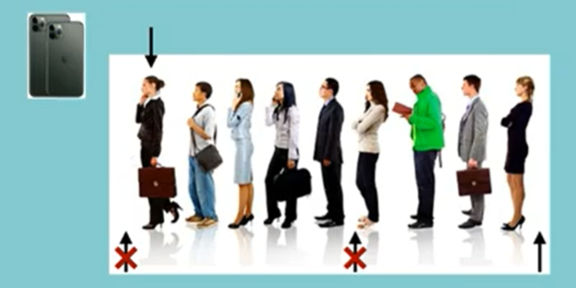
\includegraphics[width=\linewidth,keepaspectratio]{queue1.png}
\end{center}

\end{frame}

%%%%%%%%%%%%%%%%%%%%%%%%%%%%%%%%%%%%%%%%%%%%%%%%%%%%%%%%%%%%%%%%%%%%%%
\begin{frame}
	\frametitle{The Queue ADT*}
	
			\begin{itemize}

				\item Queue:
								\begin{itemize}

				\item \texttt{size()} (or \texttt{len(s)}) to get the number of items in the queue.
				\item \texttt{enqueue(item)} to add something to the queue.
				\item \texttt{dequeue()} to remove the first element from the queue.
				\item \texttt{peek()} to view the first element of the queue.
			\end{itemize}
			\item Data Structure:
			What kind of data structure should we use to implement a Queue?
				\begin{itemize}
					\item An array
					\item A python list
					\item A linked list
					\item A dict
				\end{itemize}
			\item 
			Only removing on one end and adding on the other? Seems like a DLL will do.
				\end{itemize}

						{*\scriptsize An ADT, or Abstract Data Type, is a description of the behaviour of a data structure.}
\end{frame}

%%%%%%%%%%%%%%%%%%%%%%%%%%%%%%%%%%%%%%%%%%%%%%%%%%%%%%%%%%%%%%%%%%%%%%
\begin{frame}
	\frametitle{Implementing a Linked-List based Queue}
			\begin{tabular}{r | c c}
				Queue operation & DLL operation & Time Complexity \\
				\midrule
				\texttt{size} & \texttt{size} & $O(1)$ \\
				\texttt{enqueue} & \texttt{add\_last} & $O(1)$ \\
				\texttt{dequeue}  & \texttt{remove\_first} & $O(1)$ \\
				\texttt{peek}  & \texttt{head} & $O(1)$ \\
			\end{tabular}
		

				\begin{itemize}
					\item Could we also do this using an array-based list?	
					\item What about an SLL?
					\item No more growing: 	Sure, but only for fixed capacity queues.
					\item Eeyore:	Only if we have the tail pointer.
				\end{itemize}

\end{frame}

%%%%%%%%%%%%%%%%%%%%%%%%%%%%%%%%%%%%%%%%%%%%%%%%%%%%%%%%%%%%%%%%%%%%%%
\begin{frame}
	\frametitle{Why a queue}
		In snake \ldots
			\begin{itemize}
				\item In snake, the body of the snake follows the head.
				\item If we first go left, then right, then every part of the body also needs to go first left then right.
				\item This is like a queue!
			\end{itemize}
		
			Many others?:	But of course there are many other real-world examples.
				\begin{itemize}
					\item Ticket counters,
					\item Traffic jams,
					\item Coffee machines and printers,
					\item Take-out restaurants,
					\item etc.
				\end{itemize}
\end{frame}

%%%%%%%%%%%%%%%%%%%%%%%%%%%%%%%%%%%%%%%%%%%%%%%%%%%%%%%%%%%%%%%%%%%%%
\begin{frame}
	\frametitle{Double-Ended Queues: Deques}
		\begin{itemize}
		\item Deques, or Double-Ended Queues, allow both FIFO and LIFO operations in $O(1)$ time.
		\item Hang on \ldots: 	Doesn't that sound familiar?	
		\item Back to DLL: 	This is exactly what a DLL offers!
		\end{itemize}
\end{frame}

%%%%%%%%%%%%%%%%%%%%%%%%%%%%%%%%%%%%%%%%%%%%%%%%%%%%%%%%%%%%%%%%%%%%%%
\begin{frame}
	\frametitle{\texttt{deque}}
	
	In python we can use a \texttt{deque} called \texttt{d} on which:
	\begin{itemize}
		\item We can \textit{push} with \texttt{d.append}.
		\item We can \textit{pop} with \texttt{d.pop}.
		\item We can \textit{top} with \texttt{d[-1]}
			
		\item We can \textit{enqueue} with \texttt{d.append}.
		\item We can \textit{dequeue} with \texttt{d.popleft}.
		\item We can \textit{peek} with \texttt{d[0]}
			
		\item Oh yeah and if you want, you can also add to the left with \texttt{appendleft}
	\end{itemize}
\end{frame}


%%%%%%%%%%%%%%%%%%%%%%%%%%%%%%%%%%%%%%%%%%%%%%%%%%%%%%%%%%%%%%%%%%%%%%
\begin{frame}[fragile]\frametitle{}
\begin{center}
{\Large Stack}
\end{center}

\end{frame}


%%%%%%%%%%%%%%%%%%%%%%%%%%%%%%%%%%%%%%%%%%%%%%%%%%%%%%%%%%%%%%%%%%%%%%
\begin{frame}
	\frametitle{Stacks: Me and my books}

	\begin{columns}[T]
		\column{0.455\linewidth}
			\begin{center}

					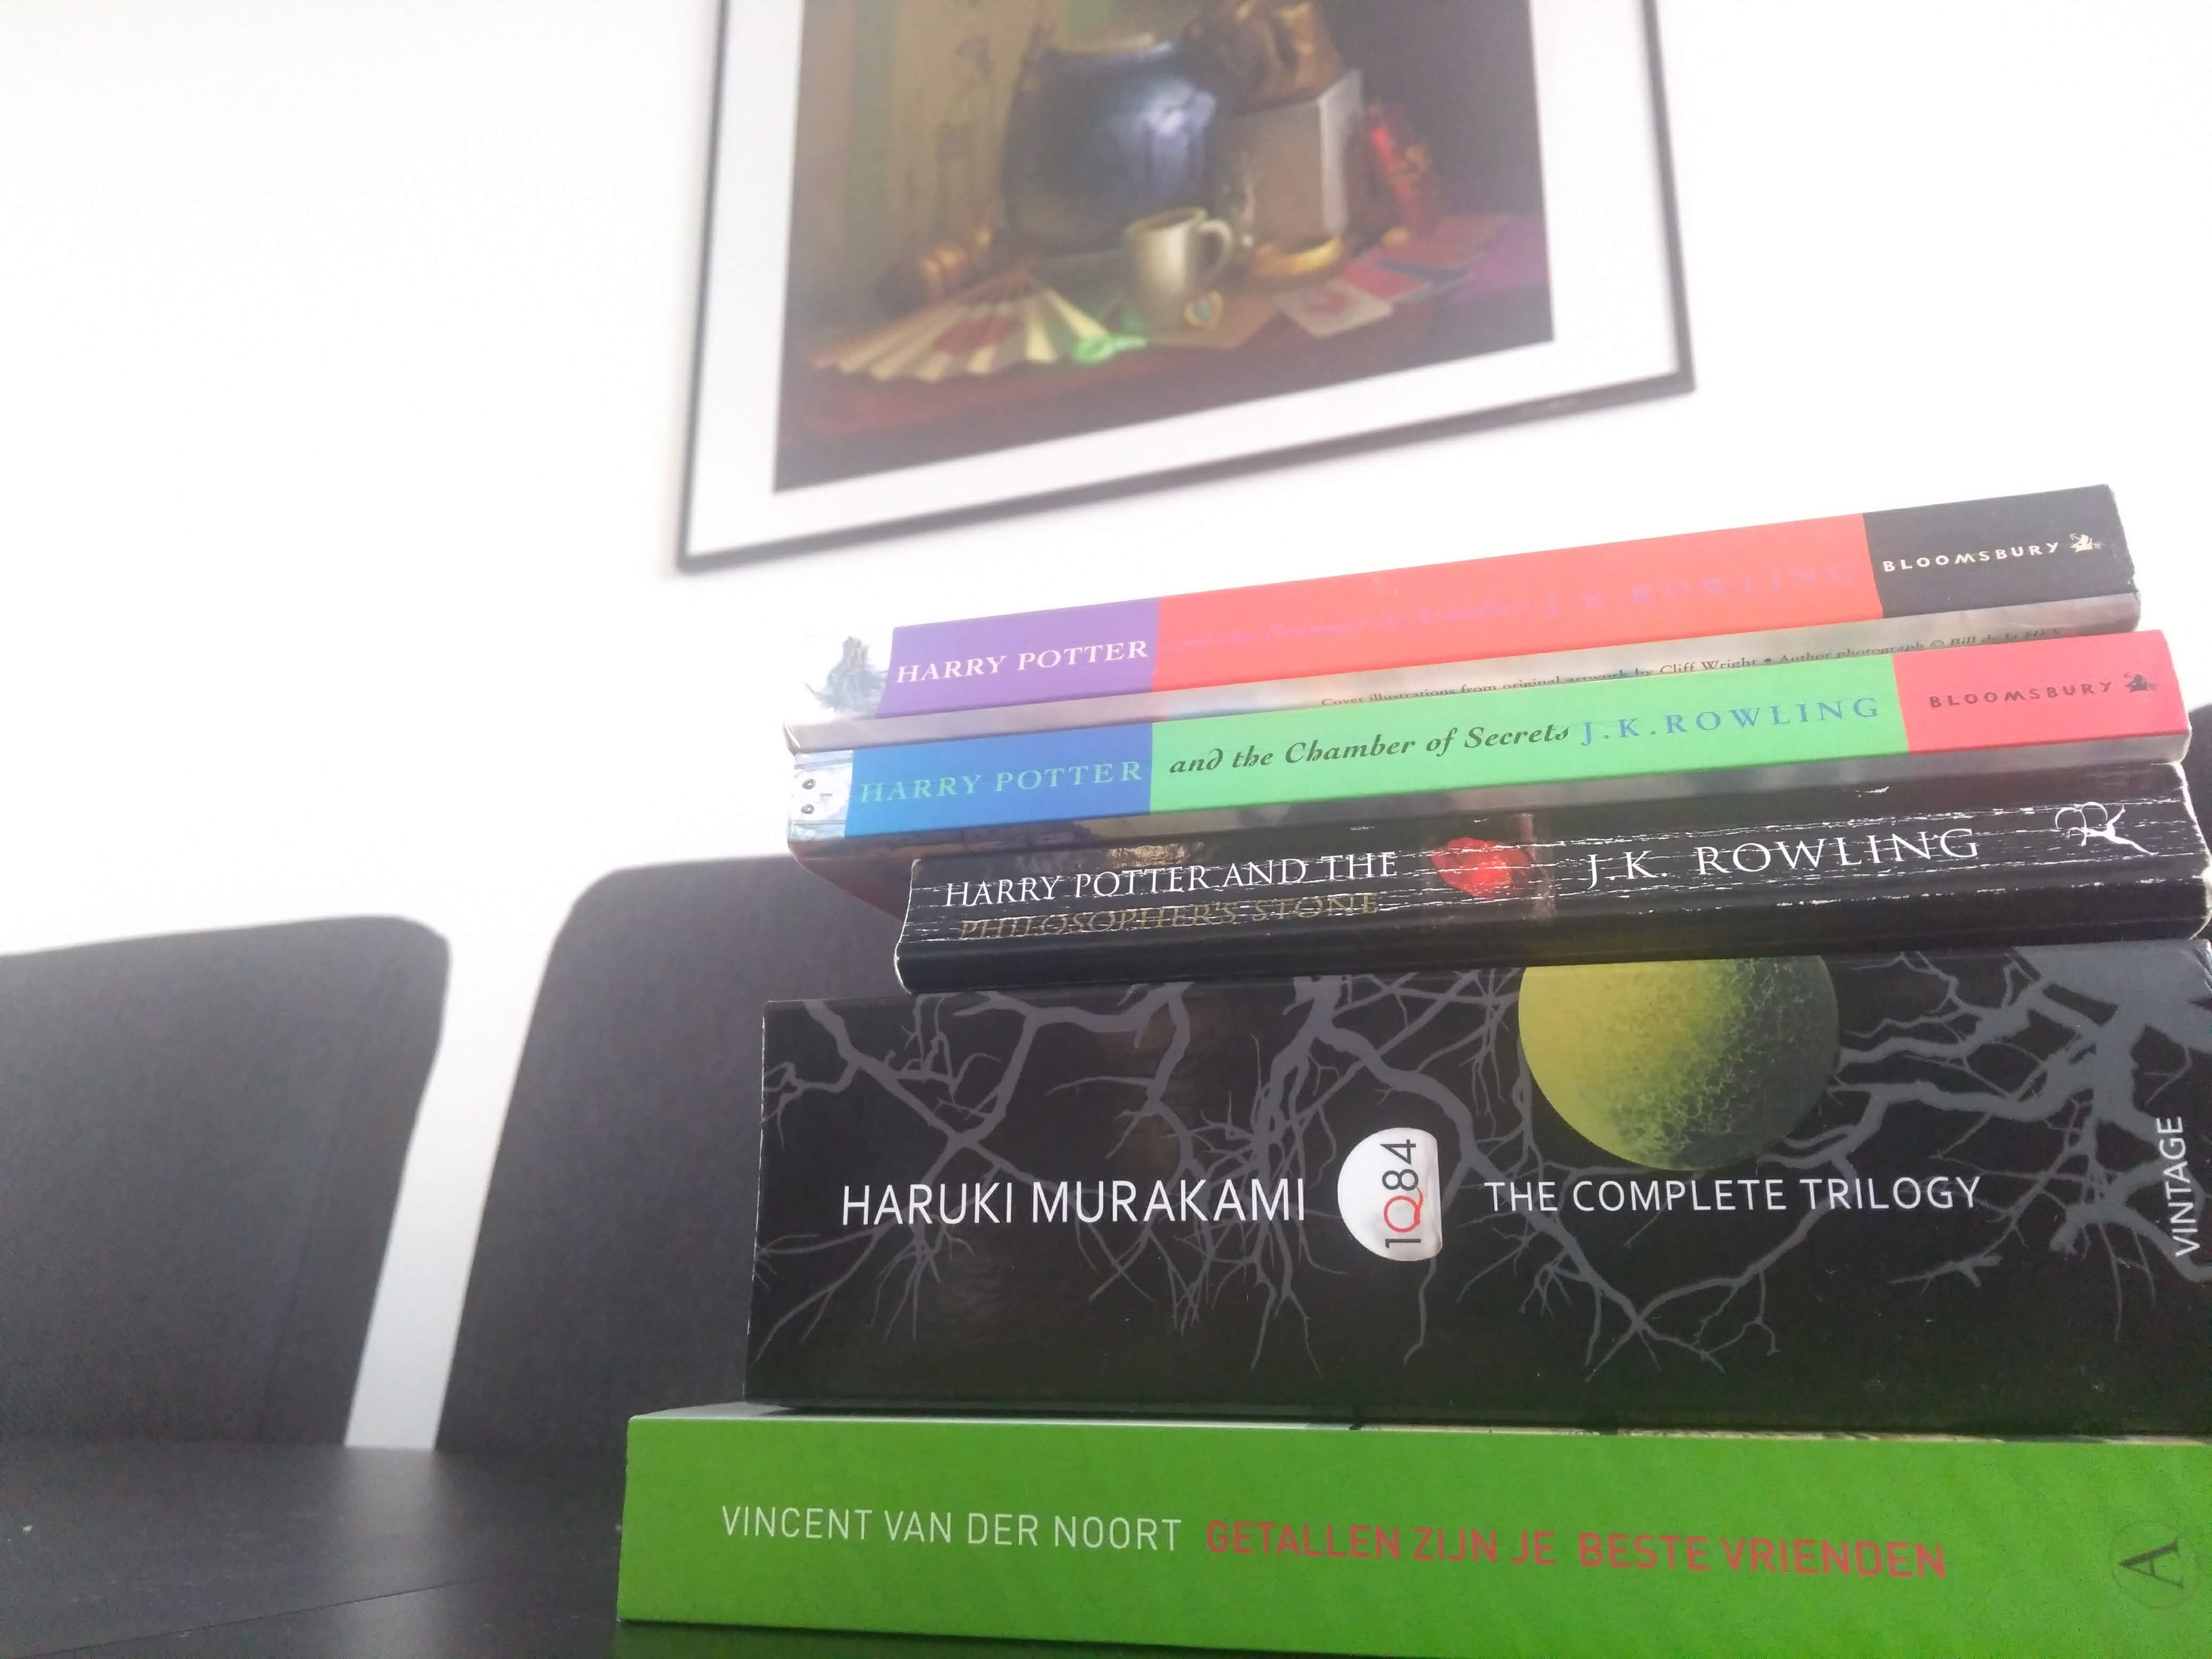
\includegraphics[width=0.7\linewidth]{images/stack_read.jpg}\\

					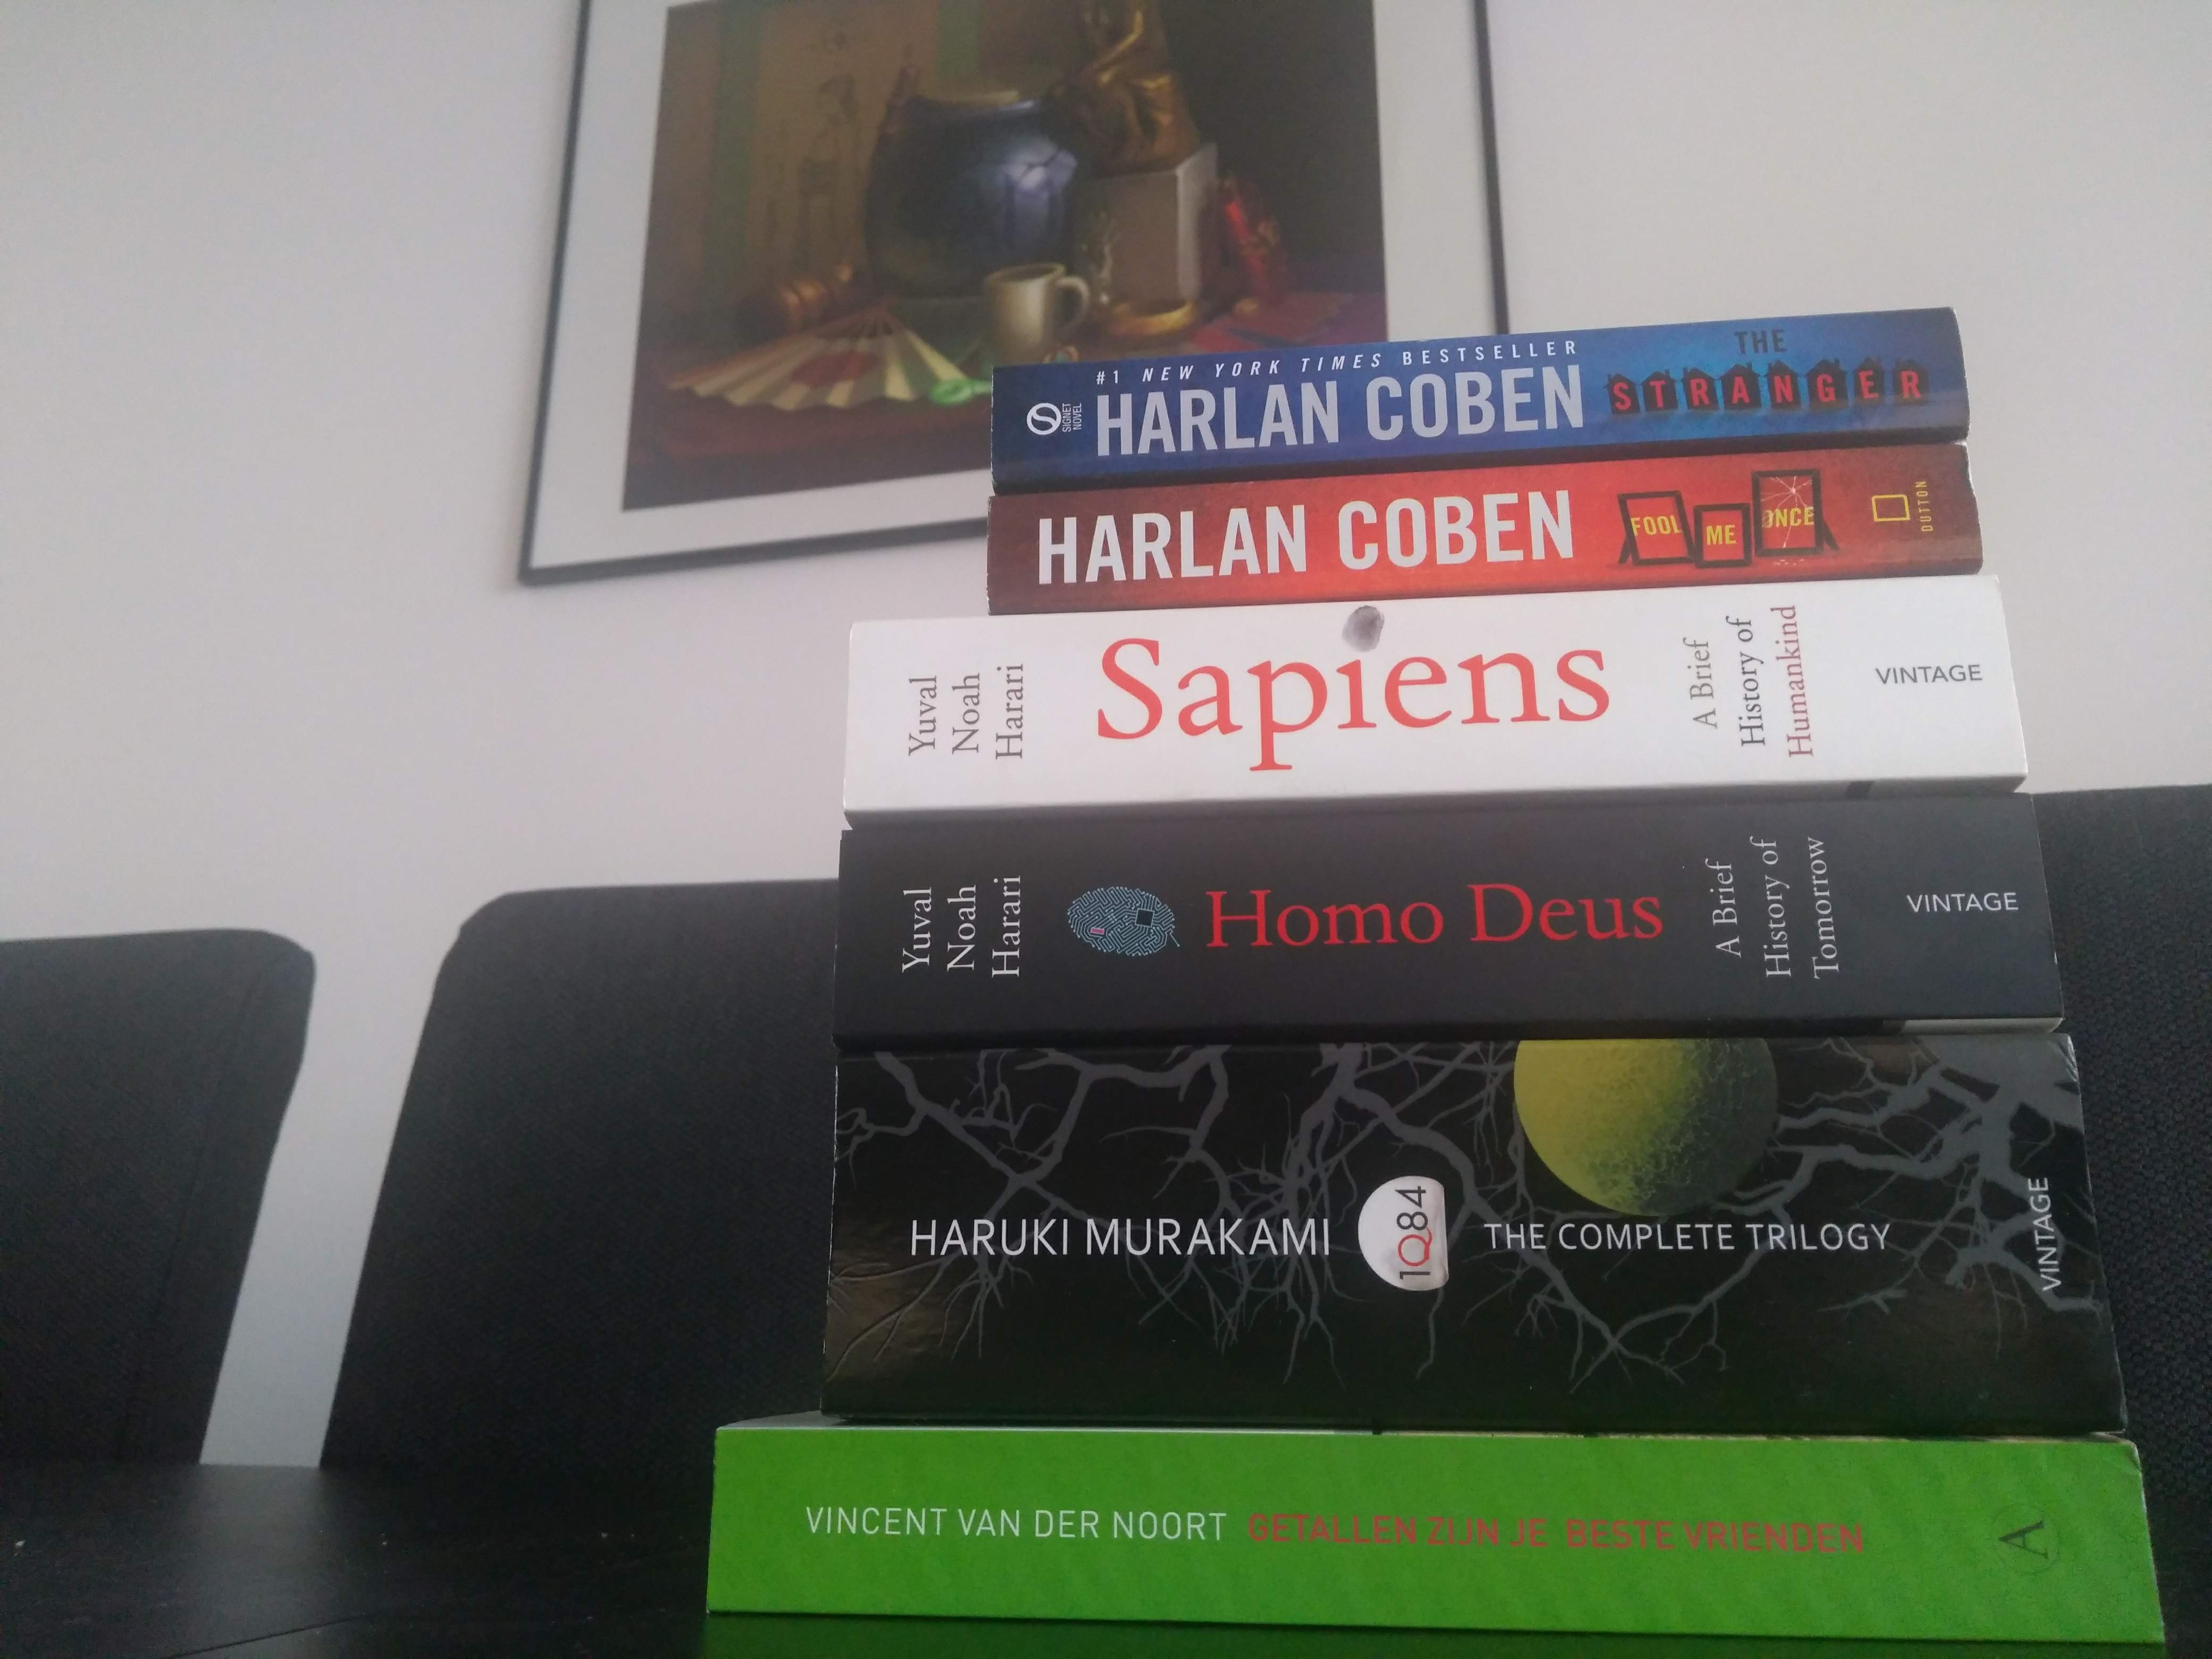
\includegraphics[width=0.7\linewidth]{images/stack_unread.jpg}\\

{\scriptsize Image By:\thinspace{\itshape Stefan Hugtenburg}}
{\scriptsize Book covers and picture in the back by others}
			\end{center}
		\column{0.455\linewidth}
		\begin{itemize}
			\item This is how I used to store books I still wanted to read.
			\item A nice \alert{stack} of books, with new ones going on the top.
			\item After finishing one, I would take the next one from the top.
			\item So after a few weeks\dots
			\item This uses the \alert{LIFO}-principle.
		\end{itemize}
	\end{columns}
\end{frame}

%%%%%%%%%%%%%%%%%%%%%%%%%%%%%%%%%%%%%%%%%%%%%%%%%%%%%%%%%%%%%%%%%%%%%%
\begin{frame}
	\frametitle{LIFO: what!?}
		\begin{itemize}
			\item The \textit{Last-In-First-Out}, or LIFO, principle is the working of a stack.
			\item The last thing we've added to the stack is the first thing we take out.
			\item Similarly the first we have added to the stack, is the last to be taken out.
		\end{itemize}	
\end{frame}

%%%%%%%%%%%%%%%%%%%%%%%%%%%%%%%%%%%%%%%%%%%%%%%%%%%%%%%%%%%%%%%%%%%%%
\begin{frame}
	\frametitle{Stack}
		\begin{itemize}
		\item Sequential collection with LIFO (Last In First Out) principle
		\item Push and Pop
		\item E.g. 'Back' button after you have visited a few websites.
		\end{itemize}
		
\begin{center}
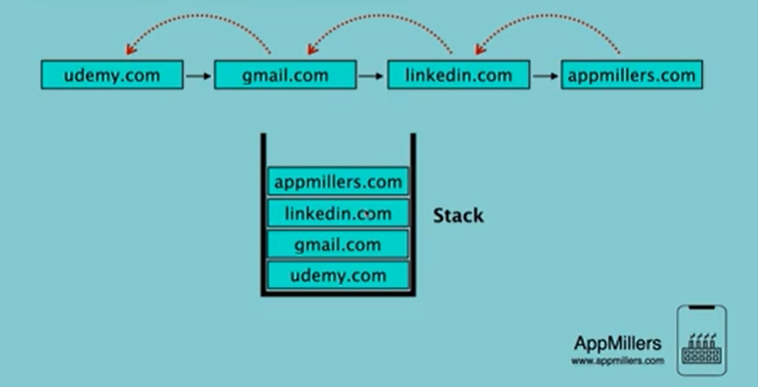
\includegraphics[width=\linewidth,keepaspectratio]{stack1.png}
\end{center}

\end{frame}


%%%%%%%%%%%%%%%%%%%%%%%%%%%%%%%%%%%%%%%%%%%%%%%%%%%%%%%%%%%%%%%%%%%%%%
\begin{frame}
	\frametitle{The Stack ADT*}
		\begin{itemize}
			\item The Stack:
				\begin{itemize}
					\item \texttt{size()} (or \texttt{len(s)}) to get the number of items in the stack.
					\item \texttt{push(item)} to add something to the stack.
						
					\item \texttt{pop()} to remove the top element from the stack.
					\item \texttt{top()} to view the top element of the stack.
				\end{itemize}
			\item Data structure?: 
				What kind of data structure should we use to implement a Stack?

				\begin{itemize}
					\item An array
					\item A python list
					\item A linked list
					\item A dict
				\end{itemize}
			\item One end only:
				Only removing and adding on one end? Seems like a DLL will do.
			\end{itemize}

						{*\scriptsize An ADT, or Abstract Data Type, is a description of the behaviour of a data structure.}
\end{frame}

%%%%%%%%%%%%%%%%%%%%%%%%%%%%%%%%%%%%%%%%%%%%%%%%%%%%%%%%%%%%%%%%%%%%%%
\begin{frame}
	\frametitle{Implementing a Linked-List based Stack}
			\begin{tabular}{r | c c}
				Stack operation & DLL operation & Time Complexity \\
				\midrule
				\texttt{size} & \texttt{size} & $O(1)$ \\
				\texttt{push} & \texttt{add\_last} & $O(1)$ \\
				\texttt{pop}  & \texttt{remove\_last} & $O(1)$ \\
				\texttt{top}  & \texttt{tail} & $O(1)$ \\
			\end{tabular}
		
				\begin{itemize}
					\item Could we also do this using an array-based list?	
					\item What about an SLL?
					\item Sure, but it's only amortised $O(1)$. So why would we?
					\item Front = Back: Sure, but we add and remove from the front!
			\end{itemize}

\end{frame}


	% %%%%%%%%%%%%%%%%%%%%%%%%%%%%%%%%%%%%%%%%%%%%%%%%%%%%%%%%%%%%%%%%%%%%%%
\begin{frame}[fragile]\frametitle{}
\begin{center}
{\Large Maps}
\end{center}

\end{frame}

%%%%%%%%%%%%%%%%%%%%%%%%%%%%%%%%%%%%%%%%%%%%%%%%%%%%%%%%%%%%%%%%%%%%%%
\begin{frame}
	\frametitle{The map ADT}
	
Maps work on \textit{key-value} pairs, usually denoted as tuples: $(k,v)$.
			
			\begin{itemize}
				\item \texttt{M.size()} (or \texttt{len(M)}) to get the number of tuples in the map.
					
				\item \texttt{M.get(k)} (or \texttt{M[k]}) to retrieve the value for key $k$.
				\item \texttt{M.put(k,v)} (or \texttt{M[k] = v}) to set the value for key $k$ to $v$.
					
				\item \texttt{M.remove(k)} (or \texttt{del M[k]}) to remove the tuple with key $k$.
					
				\item \texttt{M.contains(k)} (or \texttt{k in M}) to determine if there is tuple with key $k$.
			\end{itemize}

\end{frame}

%%%%%%%%%%%%%%%%%%%%%%%%%%%%%%%%%%%%%%%%%%%%%%%%%%%%%%%%%%%%%%%%%%%%%%
\begin{frame}
	\frametitle{A naive implementation: Listing a map}

			\begin{itemize}
				\item Why not just use a list?: If we use a list to implement the map where we just throw in all the tuples, what would the time complexity
		of the functions \texttt{get}, \texttt{remove}, \texttt{contains} be?
						\item Which?
		\begin{itemize}
			\item $\Theta(1)$
			\item $\Theta(\log n)$
			\item $\Theta(n)$
			\item $\Theta(n^2)$
			\item I don't know
		\end{itemize}
		
				\item Not so great:		All would take linear time! 
 				\item We would just have to check all the objects every time!
	\end{itemize}
\end{frame}

%%%%%%%%%%%%%%%%%%%%%%%%%%%%%%%%%%%%%%%%%%%%%%%%%%%%%%%%%%%%%%%%%%%%%%
\begin{frame}
	\frametitle{Can we do better?}
		\begin{itemize}
			\item Can we do better, and if so how?
			\item How about we try to use an array-based structure where the key determines the index?
			\item This allows for $\Theta(1)$ operations for getting, removing or checking an item!
			\item But what if the key is not integer?
	\end{itemize}
\end{frame}

%%%%%%%%%%%%%%%%%%%%%%%%%%%%%%%%%%%%%%%%%%%%%%%%%%%%%%%%%%%%%%%%%%%%%%
\begin{frame}
	\frametitle{Hash functions}
	
		\begin{itemize}
			\item Hash functions map each key $k$ to a an integer in a range $[0, N-1]$ for some $N$.
			\item Consider the hash function $f(k) = 1$ for any key $k$.
			Is this a hash function for $N=100$?
			\begin{itemize}
				\item Yes
				\item No
				\item I don't know
			\end{itemize}
			\item It is a hash function, but a terrible one!
				Why?
		\end{itemize}	
\end{frame}

%%%%%%%%%%%%%%%%%%%%%%%%%%%%%%%%%%%%%%%%%%%%%%%%%%%%%%%%%%%%%%%%%%%%%
\begin{frame}
	\frametitle{Hash to determine the index}

		\begin{itemize}
			\item We want to use hash functions to map keys to a certain index in a hash table.
			\item Back to hundred-acre woods:
		Take $f(p) = 1$, $f(i) = 3$, $f(g) = 2$, $f(l) = 8$, $f(e) = 5$, $f(t) = 7$.
		
			\item This would create the hash table:
		\begin{center}
			\begin{tikzpicture}[scale=0.85, transform shape]
	\foreach \x/\val in {0/,1/p,2/g,3/i,4/,5/e,6/,7/t,8/l,9/,10/}{
	\node[olive] (index) at (\x,1) {\x};
	\node[draw,rectangle, fill=gray!10, minimum size =1cm] (c) at (\x,0) {\val};
}
\node[] at (-2,1) {Indices:};
\node[] at (-2,0) {Array:};
\end{tikzpicture}

		\end{center}
\item The simple mapping:
		But what if we have conflicts? Like by taking $f(k)=1$ for all $k$.
	\end{itemize}	
\end{frame}

%%%%%%%%%%%%%%%%%%%%%%%%%%%%%%%%%%%%%%%%%%%%%%%%%%%%%%%%%%%%%%%%%%%%%
\begin{frame}
	\frametitle{Hashing conflicts}

		\begin{itemize}
			\item We want to use hash functions to map keys to a certain index in a hash table.\\
		But what do we do if we have hashing conflicts?
			\item Back to hundred-acre woods:
		Take $f(e) = 1$, $f(y) = 3$, $f(o) = \alert{3}$, $f(r) = 8$.
		
			\item This would create the hash table:
		\begin{center}
			\begin{tikzpicture}[scale=0.85, transform shape]
	\foreach \x/\val in {0/,1/,2/,3/,4/,5/,6/,7/,8/,9/,10/}{
	\node[olive] (index) at (\x,1) {\x};
	\node[draw,rectangle, fill=gray!10, minimum size =1cm] (\x) at (\x,0) {\val};
}
\node[] at (-2,1) {Indices:};
\node[] at (-2,0) {Array:};

\node[draw,rectangle, fill=gray!10, minimum size =0.5cm] at (1,-1.5) (e) {e};
\node[draw,rectangle, fill=gray!10, minimum size =0.5cm] at (3,-1.5) (A) {y};
\node[draw,rectangle, fill=gray!10, minimum size =0.5cm] at (3,-2.5) (B){o};
\node[draw,rectangle, fill=gray!10, minimum size =0.5cm] at (8,-1.5) (r) {r};
\draw[->, ultra thick] (A) -- (B);
\draw[*->, ultra thick] (1.center) -- (e);
\draw[*->, ultra thick] (3.center) -- (A);
\draw[*->, ultra thick] (8.center) -- (r);
\end{tikzpicture}

		\end{center}
	\end{itemize}	
\end{frame}

%%%%%%%%%%%%%%%%%%%%%%%%%%%%%%%%%%%%%%%%%%%%%%%%%%%%%%%%%%%%%%%%%%%%%
\begin{frame}
	\frametitle{Hash tables}
		\begin{itemize}
			\item We have an array of a certain capacity.
		The hash of a key, determines which \textit{bucket} to use.
			\item Every entry could for instance hold a linked-list of values.
			\item What happens?:
		So for $f(k) = 1$ for all $k$, what is the time complexity of getting the right value out for our key?
		\begin{itemize}
			\item $\Theta(1)$
			\item $\Theta(\log n)$
			\item $\Theta(n)$
			\item $\Theta(n^2)$
		\end{itemize}
			\item It is still linear time! All end up in a list after all.
		\end{itemize}
\end{frame}

%%%%%%%%%%%%%%%%%%%%%%%%%%%%%%%%%%%%%%%%%%%%%%%%%%%%%%%%%%%%%%%%%%%%%
\begin{frame}
	\frametitle{Hash functions: Ideal properties}
	
		\begin{itemize}
			\item Hash functions map each key $k$ to a an integer in a range $[0, N-1]$ for some $N$.
			\item Where ideally:
			
			\begin{itemize}
				\item keys are uniformly distributed over the range.
					
				\item ($a == b) \to (\mathit{hash}(a) == \mathit{hash}(b))$ (it is deterministic).
					
				\item the hash function is `fast' to compute (preferably $O(1)$).
			\end{itemize}
			\item This indeed makes $f(k) = 1$ pretty terrible!
			\end{itemize}	
\end{frame}

%%%%%%%%%%%%%%%%%%%%%%%%%%%%%%%%%%%%%%%%%%%%%%%%%%%%%%%%%%%%%%%%%%%%%
\begin{frame}
	\frametitle{Implementing them in Python}

	Which is better?	
			\begin{itemize}
			\item The left one.
			\item The right one.
			\item I don't know.
		\end{itemize}
		
			It depends on what kind of points we expect to see!

		
	\begin{columns}[T]
		\column{0.555\textwidth}
			\lstinputlisting{src/point.py}
		
		\column{0.555\textwidth}
		\lstinputlisting[firstline=4, lastline=15]{src/point2.py}
	\end{columns}
	


		
\end{frame}

%%%%%%%%%%%%%%%%%%%%%%%%%%%%%%%%%%%%%%%%%%%%%%%%%%%%%%%%%%%%%%%%%%%%%
\begin{frame}
	\frametitle{Hashmaps}
			\begin{itemize}
			\item Implement the Map ADT using Hash tables.
			\item With a good hash function, we expect: $\Theta(1)$ insertion/deletion/retrieval.
			But worst-case they are still $\Theta(n)$.
			\item Different options to handle hash conflicts:
			\begin{itemize}
				\item Separate Chaining
				\item (Linear) Probing
			\end{itemize}
		\end{itemize}
\end{frame}

%%%%%%%%%%%%%%%%%%%%%%%%%%%%%%%%%%%%%%%%%%%%%%%%%%%%%%%%%%%%%%%%%%%%%
\begin{frame}
	\frametitle{Lets start with the basics}
	\begin{columns}[T]
		\column{0.355\textwidth}
		\begin{itemize}
			\item Creating a new hashmap
			\item Getting the size
			\item A hash function for keys in this map
			\item Getting an item
			\item Putting an item
		\end{itemize}
		So conclusion: It depends on how we put things into the buckets!\\
				Do we use the linked list? Or do we do something else?
		\column{0.555\textwidth}
		\lstinputlisting[basicstyle=\tiny\ttfamily]{src/hashmap.py}
	\end{columns}
\end{frame}


%%%%%%%%%%%%%%%%%%%%%%%%%%%%%%%%%%%%%%%%%%%%%%%%%%%%%%%%%%%%%%%%%%%%%
\begin{frame}
	\frametitle{Recap of Maps}
	
	\begin{center}
		\begin{tabular}{c | c | c}
			Operation & Expected Time & Worst-case \\
			\midrule
			\texttt{M.size()} & $\Theta(1)$& $\Theta(1)$\\
			\texttt{M.get(k)}  & $\Theta(1)$& $\Theta(n)$\\
			\texttt{M.put(k,v)} & $\Theta(1)$& $\Theta(n)$\\
			\texttt{M.remove(k)} & $\Theta(1)$& $\Theta(n)$\\
			\texttt{M.contains(k)} & $\Theta(1)$& $\Theta(n)$\\
		\end{tabular}
	\end{center}
	
What does this depend on?:	It all stands or falls with the hash function!
			\begin{itemize}
				\item Fewer hash-conflicts means better performance.
				\item Separate chaining or (linear) probing does not matter for time performance.
				\item The latter saves us some space, but is not better in terms of space or time \textit{complexity}.
			\end{itemize}
\end{frame}


	% %%%%%%%%%%%%%%%%%%%%%%%%%%%%%%%%%%%%%%%%%%%%%%%%%%%%%%%%%%%%%%%%%%%%%%
\begin{frame}[fragile]\frametitle{}
\begin{center}
{\Large Data Structures}
\end{center}

\end{frame}


%%%%%%%%%%%%%%%%%%%%%%%%%%%%%%%%%%%%%%%%%%%%%%%%%%%%%%%%%%%%%%%%%%%%%%
\begin{frame}[fragile]\frametitle{}
\begin{center}
{\Large Lists}
\end{center}

\end{frame}

\begin{frame}
	\frametitle{Lists: the most basic data structure?}
	\begin{center}
		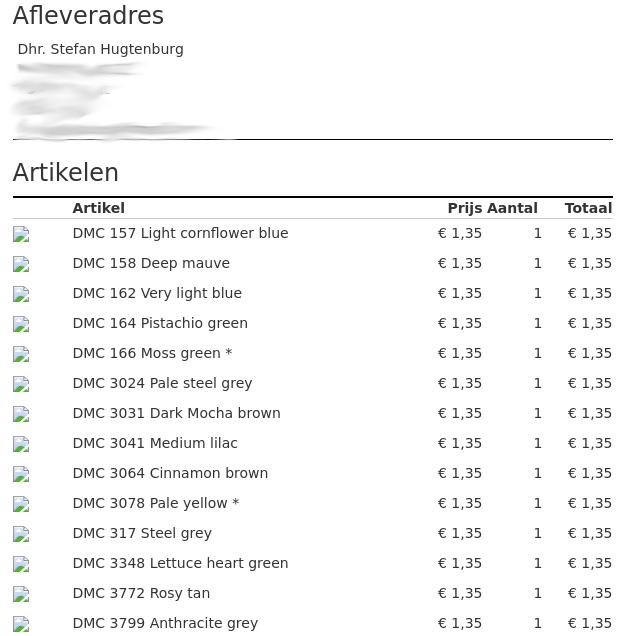
\includegraphics[width=0.8\textwidth]{images/list.png}\\
		\hspace*{15pt}\hbox{\scriptsize Screenshot By:\thinspace{\itshape Stefan Hugtenburg}}
	\end{center}
\end{frame}

\begin{frame}
	\frametitle{Why study the list?}
	\begin{block}{Use cases}
		What do we use lists for?	
	\end{block}
	\pause
	\begin{block}{Many things!}
		\begin{itemize}
			\item To store a collection of data.
				\pause
			\item To build other more complex/refined data structures!
		\end{itemize}
	\end{block}
\end{frame}

\begin{frame}
	\frametitle{Lists in Python}
	\begin{block}{Lists in Python}
		How do lists in Python work?
	\end{block}
	\pause
	\begin{block}{Arrays}
		They are array-based!
	\end{block}
	\pause
	\begin{block}{Arrays?}
		So what's an array then?
	\end{block}
\end{frame}

\begin{frame}
	\frametitle{Arrays}
	\begin{block}{Array}
		An array is a block of memory of fixed size that can hold multiple items of data.
	\end{block}	
	\pause
	\begin{columns}
		\column{0.455\textwidth}
		\vspace{10pt}
		% \begin{tikzpicture}[scale=0.85, transform shape]
	\foreach \x/\val in {0/1,1/20,2/42,3/189,4/\alt<5>{\alert{4242}}{17},5/-2}{
	\node[draw,rectangle, fill=gray!10, minimum size =1cm] (c) at (\x,0) {\val};
	\node[olive] (index) at (\x,-1) {\x};
}
\node[] at (-2,0) {Array:};
\node[] at (-2,-1) {Indices:};
\end{tikzpicture}

		\column{0.455\textwidth}
		\pause
		\begin{onlyenv}<3>

			\lstinputlisting{src/array.py}
		\end{onlyenv}
		\begin{onlyenv}<4>

			\lstinputlisting{src/array2.py}
		\end{onlyenv}
		\begin{onlyenv}<5->

			\lstinputlisting{src/array3.py}
		\end{onlyenv}
	\end{columns}
	\only<6>{
		\begin{block}{How is this different?}
			How does this differ from a list?
		\end{block}
	}
	\only<7>{
		\begin{block}{Several ways}
			\begin{itemize}
				\item It's just memory, no things like \texttt{a.sort()}.
				\item It is \textit{finite}!
			\end{itemize}
		\end{block}
	}
\end{frame}

\begin{frame}
	\frametitle{Array-based lists}
	\begin{block}{Array-based list}
		An array-based list (like the \texttt{list} in Python) uses an array internally.
	\end{block}
	\begin{block}{Growing a list?}
		How can we then grow the list (seemingly) infinitely?
		\begin{enumerate}[A.]
			\item The list uses multiple arrays stitched together.
			\item The list also has a finite size from the start, we just never notice.
			\item The list creates a new array of size $n+1$ when the array if full.
			\item The list creates a new array of size $n*2$ when the array if full.
			\item I don't know.
		\end{enumerate}
	\end{block}
\end{frame}

\begin{frame}
	\frametitle{No! Bad Frankenstein!}
	\begin{block}{Stitching arrays together}
		The list uses multiple arrays stitched together.
		\begin{itemize}
			\item Although technically possible, keeping track of all of it is hell not pleasant.
			\item There are also benefits to having one continuous block of memory.
				\begin{itemize}
					\item For instance spacial caching benefits (Google it, if you are intrigued ;))
				\end{itemize}
				\pause
			\item But the idea isn't a bad one per se. Having only single items blocks, forms the basis of the list we study
				after the break!
		\end{itemize}
	\end{block}	
\end{frame}

\begin{frame}
	\frametitle{Too infinity and beyond}
	\begin{block}{A hidden maximum size?}
		The list also has a finite size from the start, we just never notice.
		\begin{itemize}
			\item Nope, we can grow it so long as there is memory available.
		\end{itemize}
	\end{block}	
\end{frame}

\begin{frame}
	\frametitle{So... New arrays then?}
	\begin{block}{A new one!}
		When the initial array is full, we create a new one with more capacity.\\
		We copy over all existing elements into the new array\dots\\
		And we now have new space to grow!
	\end{block}	
	\pause
	\begin{block}{Question}
		But by how much should we grow?	
	\end{block}
	\pause
	\begin{block}{Observations}
		\begin{itemize}
			\item Adding one item, can trigger a full copy of the array...
			\item Does that make \texttt{append} an $O(n)$ operation?
		\end{itemize}
	\end{block}	
\end{frame}

\begin{frame}
	\frametitle{It depends}
	\begin{block}{Just enough room}
		The list creates a new array of size $n+1$ when the array if full.
	\end{block}	
	\begin{block}{Doing it often}
		What happens when we add $n$ elements to a list of size $1$?\\
		\begin{itemize}
			\item Every time we need to copy the full list.
			\item So $O(\sum\limits_{i=1}^{n}i)$ time in total.
			\item So $O(n^2)$ to add $n$ elements\dots
		\end{itemize}
	\end{block}	
\end{frame}

\begin{frame}
	\frametitle{It depends}
	\begin{block}{More than enough room}
		The list creates a new array of size $n*2$ when the array if full.
	\end{block}	
	\begin{block}{Doing it often}
		What happens when we add $n$ elements?
	\end{block}
\end{frame}

\begin{frame}
	\frametitle{Amortised run time}
	\begin{block}{Amortised run time}
		Some operations have varying run times, but can be shown to be efficient when repeated multiple times. We call
		this an amortised run time.
	\end{block}	
	\pause
	\begin{block}{Consider...}
		\small
		\begin{itemize}
			\item Consider a list of size $1$ and we add $n$ elements to it.
				\vspace{-5pt}
				\pause
			\item This means we double the size of the list $\log_2(n)$ times.
				\vspace{-5pt}
				\pause
			\item This means that in total we have: $O(n)$ time to add all elements.
				\vspace{-5pt}
				\pause
			\item And $O\left(\sum\limits_{i=1}^{\log_2(n)} 2^i\right)$ operations to copy when the list grows.
				\vspace{-5pt}
			\item This geometric sequence gets us to: $O(2^{\log_2(n)}) = O(n)$ operations.
				\vspace{-5pt}
				\pause
			\item So $O(n)$ to add $n$ items!
				\vspace{-5pt}
		\end{itemize}
		\pause
		We call this an amortised run time of $O(1)$ for the append operation!
	\end{block}	
\end{frame}

\begin{frame}
	\frametitle{Inserter}
	\begin{center}
		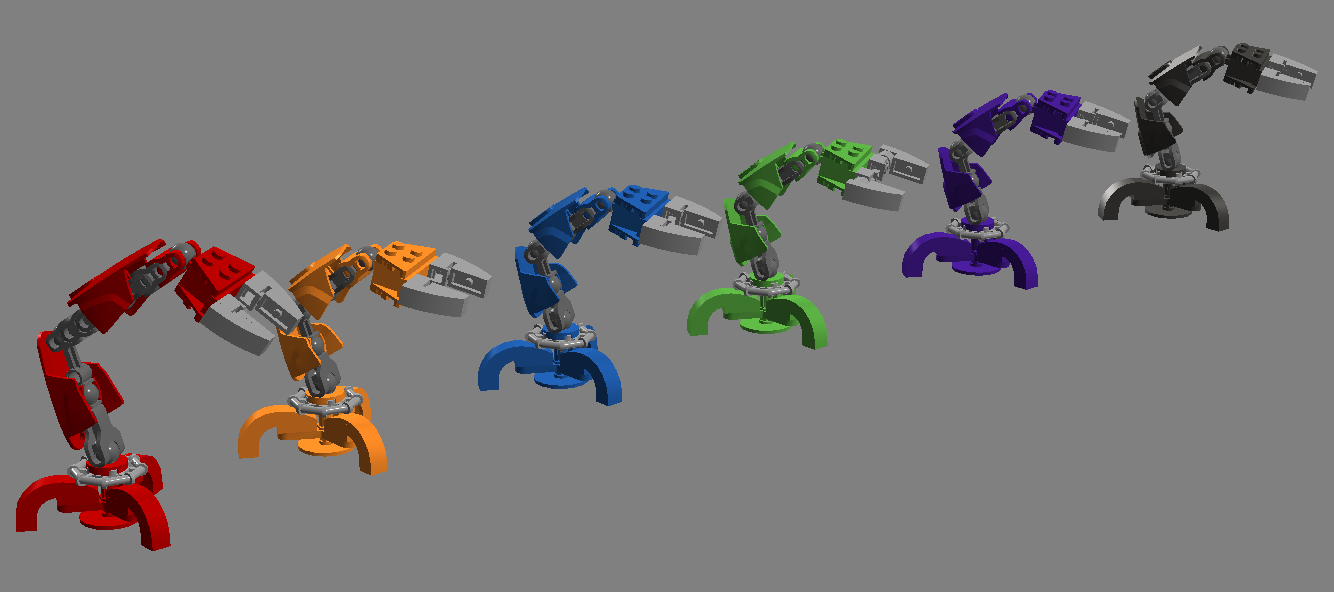
\includegraphics[width=0.8\textwidth]{images/inserter.png}\\
		\hspace*{15pt}\hbox{\scriptsize Image By:\thinspace{\itshape TheMugbearer}}
		% https://www.reddit.com/r/factorio/comments/4s015w/decided_to_also_post_a_sort_of_factorio_fanart/
	\end{center}
\end{frame}

\begin{frame}
	\frametitle{Inserting}
	\begin{columns}
		\column{0.455\textwidth}

		\begin{block}{Let's insert}
			What is the time complexity of \texttt{l.insert(index,value)} when \texttt{len(l)}=n?
			\begin{enumerate}[A.]
				\item $O(1)$
				\item $O(\textit{index})$
				\item $O(n - \textit{index})$
				\item $O(n)$
				\item $O(n^2)$
				\item I don't know.
			\end{enumerate}
		\end{block}
		\pause
		\column{0.455\textwidth}
		\begin{block}{Let's insert}
			We need to shift all elements after \texttt{index}, so $O(n-\textit{index})$
		\end{block}
		\pause
		\begin{block}{Inserting at the front}
			This means prepending is $O(n)$ for array-based lists!
		\end{block}	
	\end{columns}
\end{frame}

\begin{frame}
	\frametitle{Getting rid of the trash}
	\begin{center}
		
\includegraphics[width=0.3\textwidth]{images/trash.jpg}\\
		\hspace*{15pt}\hbox{\scriptsize Image By:\thinspace{\itshape Tgasser}}
		% https://commons.wikimedia.org/wiki/File:Trash_person.jpg
	\end{center}
\end{frame}

\begin{frame}
	\frametitle{Removing an item}
	\begin{columns}
		\column{0.455\textwidth}
		\begin{block}{Let's pop}
			What is the time complexity of \texttt{l.pop(index)} when \texttt{len(l)}=n?
			\begin{enumerate}[A.]
				\item $O(1)$
				\item $O(\textit{index})$
				\item $O(n - \textit{index})$
				\item $O(n)$
				\item $O(n^2)$
				\item I don't know.
			\end{enumerate}
		\end{block}
		\pause
		\column{0.455\textwidth}
		\begin{block}{Let's pop}
			We need to shift all elements after \texttt{index}, so $O(n-\textit{index})$.
		\end{block}
		\pause
		\begin{block}{Inserting at the front}
			This means removing the first item is $O(n)$ for array-based lists!
		\end{block}	
	\end{columns}
\end{frame}

\begin{frame}
	\frametitle{Removing an item}
	\begin{columns}
		\column{0.455\textwidth}
		\begin{block}{Let's remove}
			What is the time complexity of \texttt{l.remove(value)} when \texttt{len(l)}=n?
			\begin{enumerate}[A.]
				\item $O(1)$
				\item $O(\textit{index})$, where index is the index of the value.
				\item $O(n - \textit{index})$, where index is the index of the value.
				\item $O(n)$
				\item $O(n^2)$
				\item I don't know.
			\end{enumerate}
		\end{block}
		\pause
		\column{0.455\textwidth}
		\begin{block}{Let's remove}
			We need to find the element so $O(\textit{index})$.\\
			We need to shift all elements after \texttt{index}, so $O(n-\textit{index})$.\\
			Together this is $O(n)$.
		\end{block}
	\end{columns}
\end{frame}

\begin{frame}
	\frametitle{Freeing up memory}
	\begin{block}{Freeing up space}
		When we remove sufficient items, we can free up space again.\\
		We do this when 25\% of the capacity is used.
	\end{block}	
	\pause
	\begin{block}{Why 25\%?}
		Why not just when we drop below 50\% again?
	\end{block}
	\pause
	\begin{block}{Thrashing}
		Thrashing is repeatedly claiming and releasing memory (and in this case copying the array).\\
		To avoid this, we use a different bound on when we release memory.
	\end{block}
\end{frame}

\begin{frame}
	\frametitle{Lists in Python}
	So to summarise:
	\begin{itemize}
		\item Insert first element: $O(n)$.
		\item Insert at index $k$: $O(n-k)$.
		\item Append: amortised $O(1)$.
		\item Remove first element: $O(n)$.
		\item Remove last element: amortised $O(1)$.
		\item Remove index $k$: $O(n-k)$.
		\item Search (discussed last week): $O(n)$.
	\end{itemize}
\end{frame}

%%%%%%%%%%%%%%%%%%%%%%%%%%%%%%%%%%%%%%%%%%%%%%%%%%%%%%%%%%%%%%%%%%%%%%
\begin{frame}[fragile]\frametitle{}
\begin{center}
{\Large Linked Lists}
\end{center}

\end{frame}

\begin{frame}
	\frametitle{Linked list}
	\begin{center}
		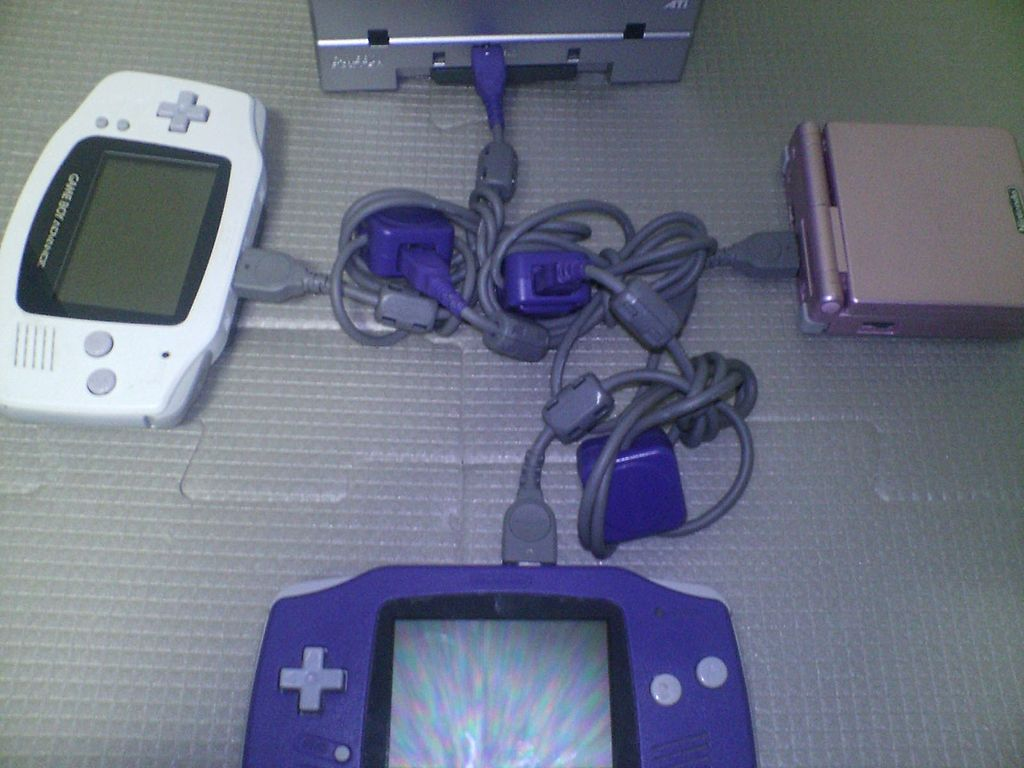
\includegraphics[width=0.6\textwidth]{images/gba.jpg}\\
		\hspace*{15pt}\hbox{\scriptsize Image By:\thinspace{\itshape PiaCarrot}}
		%https://commons.wikimedia.org/wiki/File:GBA_4PConnection.jpg
	\end{center}
\end{frame}

\begin{frame}
	\frametitle{Another approach}
	
	\begin{block}{What do we want to solve?}
		Two things in the array-based implementation that we hope to solve:
		\begin{enumerate}
			\item Only use space for items we actually use.
			\item Allow for efficient ($O(1)$?) adding and removing at the front of the list.
		\end{enumerate}
	\end{block}
	\pause
	\begin{block}{}
		Why do we want this efficient adding/removing?
	\end{block}
\end{frame}

\begin{frame}
	\frametitle{The notion of a linked list}
	\begin{columns}
		\column{0.455\textwidth}
			\begin{itemize}
				\item We build a list of blocks, starting with one item/block (we call this the \alert{head})
				\item<2-> We can then add another.
				\item<3-> These are connected, we can go from the first to the second item.
				\item<4-> So let's add one more item.
				\item<5-> We should also indicate when we have reached the end (we call this the \alert{tail}).
			\end{itemize}
		\column{0.455\textwidth}
		% % Tikz template taken from: https://tex.stackexchange.com/a/19288
\begin{tikzpicture}[list/.style={draw}]

  \node[list] (A) {42};
	\only<2->{
  \node[list] (B) {99};
}
	\only<3->{
  \draw[] let \p1 = (A.two), \p2 = (A.center) in (\x1,\y2) -- (B);
}
	\only<4->{
  \node[list] (C) {12};
  \draw[] let \p1 = (B.two), \p2 = (B.center) in (\x1,\y2) -- (C);
}
\only<5->{
  \node[draw,inner sep=6pt] (D) {};
  \draw (D.north east) -- (D.south west);
  \draw (D.north west) -- (D.south east);
  \draw[] let \p1 = (C.two), \p2 = (C.center) in (\x1,\y2) -- (D);
}
\end{tikzpicture}	

	\end{columns}
\end{frame}

\begin{frame}
	\frametitle{How does this work now?}
	\framesubtitle{Searching for an item}	
	The approach:
	\begin{enumerate}
		\item Start at the head of the list.
		\item<2-> If this is is the item we need, return True.
		\item<2-> Else if this is the tail, return False.
		\item<3-> Else, move to the next item of the list and go to step 2.
	\end{enumerate}

		% % Tikz template taken from: https://tex.stackexchange.com/a/19288
\begin{tikzpicture}[list/.style={draw}]

	\node[list,on chain,onslide=<1-2>{red}] (A) {42};
	\node[list,on chain,onslide=<3>{red}] (B) {99};
  \draw[] let \p1 = (A.two), \p2 = (A.center) in (\x1,\y2) -- (B);
  \node[list,on chain,onslide=<4>{red}] (C) {12};
  \draw[] let \p1 = (B.two), \p2 = (B.center) in (\x1,\y2) -- (C);
	\node[on chain,draw,inner sep=6pt,onslide=<5>{red}] (D) {};
	\draw[onslide=<5>{red}] (D.north east) -- (D.south west);
	\draw[onslide=<5>{red}] (D.north west) -- (D.south east);
  \draw[] let \p1 = (C.two), \p2 = (C.center) in (\x1,\y2) -- (D);
\end{tikzpicture}	

	
	\only<6->{
	\lstinputlisting{src/ll_search.py}
}
\end{frame}

\begin{frame}
	\frametitle{Getting an item!?}
	\framesubtitle{Getting item at index $i$}

	\begin{itemize}
		\item There is no easy way to access the $i$th item other than to `walk' there.
		\item So $O(\textit{index})$ to get the item at a certain \texttt{index}.
	\end{itemize}
	\lstinputlisting{src/ll_get.py}
\end{frame}

\begin{frame}
	\frametitle{Inserting at the head or tail}
	\begin{itemize}
		\item Take the current head or tail.
		\item And put the new node before or after it :)
		\item<4-> \alert{$O(1)$ time!}
	\end{itemize}	
	\begin{columns}[t]
		\column{0.535\textwidth}
	\only<2->{
		\lstinputlisting{src/ll_prepend.py}
	}
		\column{0.535\textwidth}
	\only<3->{
		\lstinputlisting{src/ll_append.py}
	}
			
	\end{columns}
\end{frame}

\begin{frame}
	\frametitle{Assumptions, Assumptions}
	\begin{block}{Unfortunately}
		To do \texttt{add\_last} in constant time, we need a reference to the \texttt{tail}.\\
		Many implementations of Singly-Linked Lists do not have this.
	\end{block}		
	\pause
	\begin{block}{Wait Singly?}
		What do I mean with `Singly' Linked List?	
	\end{block}
	\pause
	\begin{block}{Well, it's not doubly linked}
		In other implementations, we can both go forwards and backwards!	
	\end{block}
\end{frame}

\begin{frame}
	\frametitle{Doubly-Linked Lists}
	\begin{overlayarea}{\textwidth}{0.5\textheight}
		% \begin{center}
			% % Tikz template taken from: https://tex.stackexchange.com/a/19288
\begin{tikzpicture}[list/.style={rectangle split, rectangle split parts=2,
    draw, rectangle split horizontal}, >=stealth, start chain]

  \node[list,on chain] (A) {42};
  \node[list,on chain] (B) {99};
  \draw[*->] let \p1 = (A.two), \p2 = (A.center) in (\x1,\y2) -- (B);
  \node[list,on chain] (C) {12};
  \draw[*->] let \p1 = (B.two), \p2 = (B.center) in (\x1,\y2) -- (C);
  \node[on chain,draw,inner sep=6pt] (D) {};
  \draw (D.north east) -- (D.south west);
  \draw (D.north west) -- (D.south east);
  \draw[*->] let \p1 = (C.two), \p2 = (C.center) in (\x1,\y2) -- (D);

\end{tikzpicture}	

		% \end{center}
		\only<1->{
			\begin{block}{A singly linked list}
				Only has connections in one direction.	
			\end{block}	
		}
		\only<2>{
			% \begin{center}
				% % Tikz template taken from: https://tex.stackexchange.com/a/19288
\begin{tikzpicture}[list/.style={rectangle split, rectangle split parts=2,
    draw, rectangle split horizontal},start chain]

		\only<2->{
  \node[on chain,draw,inner sep=6pt] (E) {};
  \draw (E.north east) -- (E.south west);
  \draw (E.north west) -- (E.south east);
}
  \node[list,on chain] (A) {42};
  \node[list,on chain] (B) {99};
  \draw[*->] let \p1 = (A.two), \p2 = (A.center) in (\x1,\y2) -- (B);
  \node[list,on chain] (C) {12};
  \draw[*->] let \p1 = (B.two), \p2 = (B.center) in (\x1,\y2) -- (C);
  \node[on chain,draw,inner sep=6pt] (D) {};
  \draw (D.north east) -- (D.south west);
  \draw (D.north west) -- (D.south east);
  \draw[*->] let \p1 = (C.two), \p2 = (C.center) in (\x1,\y2) -- (D);

	\only<2->{
		\draw[->,red,thick] let \p1 = (A.two), \p2 = (A.center) in (B) to [out=150, in=30] (\x1,\y2);
		\draw[->,red,thick] let \p1 = (B.two), \p2 = (B.center) in (C) to [out=150, in=30] (\x1,\y2);
		\draw[->,red,thick] let \p1 = (E.center), \p2 = (E.center) in (A) to [out=150, in=30] (\x1,\y2);
	}
\end{tikzpicture}	

			% \end{center}
			\begin{block}{A doubly linked list}
				Has connections in both directions.
			\end{block}
		}
	\end{overlayarea}
\end{frame}

\begin{frame}
	\frametitle{Inserting an item}
	\framesubtitle{What to do?}
	\begin{columns}
		\column{0.255\textwidth}
	\begin{itemize}
		\item Navigate to the place where we want to insert the item ($O(\textit{index})$)
			\pause
		\item Add the item: $O(1)$
			\pause
		\item So $O(\textit{index})$ time!
	\end{itemize}
			
		\column{0.755\textwidth}
		\pause
	\lstinputlisting{src/ll_insert.py}
			
	\end{columns}
\end{frame}

\begin{frame}
	\frametitle{Removing an item}
	\begin{block}{Removing an item}
		What is the time complexity of removing the first and last item in a singly linked list?
		\only<1>{
		\begin{enumerate}[A.]
			\item $O(1)$ for the first, $O(1)$ for the last.
			\item $O(1)$ for the first, $O(n)$ for the last.
			\item $O(n)$ for the first, $O(1)$ for the last.
			\item $O(n)$ for the first, $O(n)$ for the last.
			\item I don't know.
		\end{enumerate}
	}
	\end{block}
	\vspace{-20pt}
	\begin{columns}[t]
		
		\column{0.535\textwidth}
	\only<2->{
		\lstinputlisting{src/ll_remove_first.py}
	\vspace{-5pt}
		$O(1)$ time.
	}
		\column{0.535\textwidth}
	\only<3->{
		\lstinputlisting{src/ll_remove_last.py}
	\vspace{-5pt}
		$O(n)$ time.
	}
	\end{columns}
	
\end{frame}

\begin{frame}
	\frametitle{Improvements!}
		\begin{block}{Doubly-linked list remove last}
			Note that in a doubly-linked list we can remove the last item in $O(1)$ time!\\
			We can just use \texttt{tail.prev} to find the last-but-one element in constant time!\\
		\end{block}	
\end{frame}

\begin{frame}
	\frametitle{So to summarise}
\begin{columns}
	\column{0.655\textwidth}
	\begin{tabular}{l | c | c | c}
	Operation & Array-based list & SLL & DLL \\	
	\midrule
	Get element $k$ & $O(1)$ &$O(k)$ & $O(k)$ \\
	\pause
	Insert first element& $O(n)$ & $O(1)$ & $O(1)$\\
	Insert at index $k$& $O(n-k)$ & $O(k)$ & $O(\min(k,n-k))$\\
	Append (amortised)& $O(1)$ & $O(1)$ & $O(1)$\\
	\pause
	Remove first element& $O(n)$ & $O(1)$ & $O(1)$\\
	Remove last element& $O(1)$ & $O(n)$ & $O(1)$\\
	Remove index $k$& $O(n-k)$ & $O(k)$ & $O(\min(k,n-k))$\\
	\pause
	Search & $O(n)$ & $O(n)$ & $O(n)$\\
	\end{tabular}
		
	\column{0.355\textwidth}
%	\pause
%	\begin{block}{Which should you use?}
%		So which is better?	
%	\end{block}
%	\pause
%	\begin{block}{It depends!}
%		But on what?	
%	\end{block}
		
\end{columns}

\end{frame}

%%%%%%%%%%%%%%%%%%%%%%%%%%%%%%%%%%%%%%%%%%%%%%%%%%%%%%%%%%%%%%%%%%%%%%
\begin{frame}[fragile]\frametitle{}
\begin{center}
{\Large Queue}
\end{center}

\end{frame}

\begin{frame}
	\frametitle{The Queue ADT}
	\begin{overlayarea}{\textwidth}{\textheight}
		\begin{block}{The Queue}
			\begin{itemize}
				\item \texttt{size()} (or \texttt{len(s)}) to get the number of items in the queue.
				\item \texttt{enqueue(item)} to add something to the queue.
					\pause
				\item \texttt{dequeue()} to remove the first element from the queue.
				\item \texttt{peek()} to view the first element of the queue.
			\end{itemize}
		\end{block}	
		\pause
		\begin{block}{Data structure?}
			What kind of data structure should we use to implement a Queue?
				\only<3>{
				\begin{enumerate}[A.]
					\item An array
					\item A python list
					\item A linked list
					\item A dict
				\end{enumerate}
			}
		\end{block}
		\pause
		\begin{block}{One end only}
			Only removing on one end and adding on the other? Seems like a DLL will do.
		\end{block}
	\end{overlayarea}
\end{frame}

\begin{frame}
	\frametitle{Implementing a Linked-List based Queue}
	\begin{overlayarea}{\textwidth}{\textheight}
			\begin{tabular}{r | c c}
				Queue operation & DLL operation & Time Complexity \\
				\midrule
				\texttt{size} & \only<2->{\texttt{size} & $O(1)$} \\
				\texttt{enqueue} & \only<2->{\texttt{add\_last} & $O(1)$} \\
				\texttt{dequeue}  & \only<2->{\texttt{remove\_first} & $O(1)$} \\
				\texttt{peek}  & \only<2->{\texttt{head} & $O(1)$} \\
			\end{tabular}
		
			\begin{columns}[t]
				\column{0.455\textwidth}
			\only<3->{
			\begin{block}{Arrays}
				Could we also do this using an array-based list?	
			\end{block}
		}
			\only<5->{
			\begin{block}{SLL}
				What about an SLL?
			\end{block}
		}
				\column{0.455\textwidth}
				\only<4->{
				\begin{block}{No more growing}
					Sure, but only for fixed capacity queues.
				\end{block}
				}
				\only<6->{
				\begin{block}{Eeyore}
					Only if we have the tail pointer.
				\end{block}
				}
		
			\end{columns}
	\end{overlayarea}
\end{frame}

\begin{frame}
	\frametitle{Snake games}
	\framesubtitle{Nostalgia overload}
	\begin{center}
		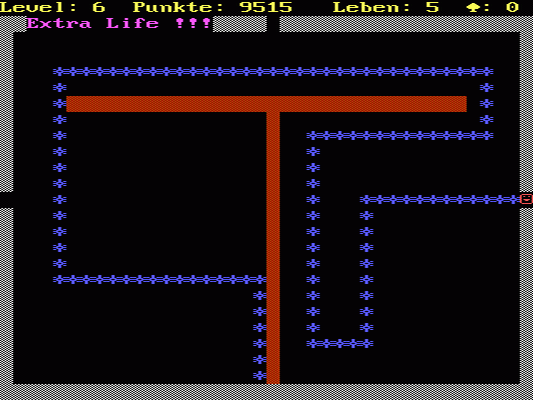
\includegraphics[width=0.6\textwidth]{images/snake.png}\\
		\hspace*{15pt}\hbox{\scriptsize Image By:\thinspace{\itshape Thomas Jensen}}
	\end{center}
	% https://commons.wikimedia.org/wiki/File:Cgasnake.png 
\end{frame}

\begin{frame}
	\frametitle{Why a queue}
		\begin{block}{In snake...}
			\begin{itemize}
				\item In snake, the body of the snake follows the head.
					\pause
				\item If we first go left, then right, then every part of the body also needs to go first left then right.
					\pause
				\item This is like a queue!
			\end{itemize}
		\end{block}	
		\pause
			\begin{block}{Many others?}
				But of course there are many other real-world examples.
				\begin{itemize}
					\item Ticket counters,
					\item Traffic jams,
					\item Coffee machines and printers,
					\item Take-out restaurants,
					\item etc.
				\end{itemize}
			\end{block}	
\end{frame}

\begin{frame}
	\frametitle{Double-Ended Queues}

	\begin{center}
		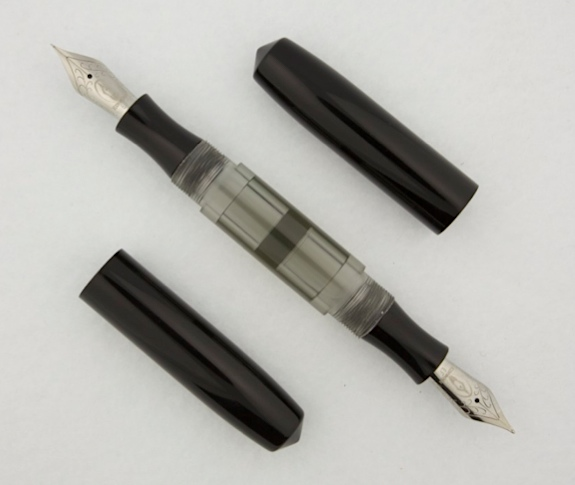
\includegraphics[width=0.5\textwidth]{images/de.jpg}\\
		\hspace*{15pt}\hbox{\scriptsize Image By:\thinspace{\itshape Chris Lott}}
		% https://www.flickr.com/photos/fncll/9824392125
	\end{center}
\end{frame}

\begin{frame}
	\frametitle{Deques}
		\begin{block}{Deques}
			Deques, or Double-Ended Queues, allow both FIFO and LIFO operations in $O(1)$ time.
		\end{block}		
		\pause
		\begin{block}{Hang on...}
			Doesn't that sound familiar?	
		\end{block}
		\pause
		\begin{block}{Back to DLL}
			This is exactly what a DLL offers!
		\end{block}
\end{frame}

\begin{frame}
	\frametitle{\texttt{deque}}
	
	In python we can use a \texttt{deque} called \texttt{d} on which:
	\begin{itemize}
		\item We can \textit{push} with \texttt{d.append}.
		\item We can \textit{pop} with \texttt{d.pop}.
		\item We can \textit{top} with \texttt{d[-1]}
			\pause
		\item We can \textit{enqueue} with \texttt{d.append}.
		\item We can \textit{dequeue} with \texttt{d.popleft}.
		\item We can \textit{peek} with \texttt{d[0]}
			\pause
		\item Oh yeah and if you want, you can also add to the left with \texttt{appendleft}
	\end{itemize}
\end{frame}


%%%%%%%%%%%%%%%%%%%%%%%%%%%%%%%%%%%%%%%%%%%%%%%%%%%%%%%%%%%%%%%%%%%%%%
\begin{frame}[fragile]\frametitle{}
\begin{center}
{\Large Stack}
\end{center}

\end{frame}


\begin{frame}
	\frametitle{Stacks}
	\begin{center}
		
\includegraphics[width=0.4\textwidth]{images/stack_of_books.png}\\
		\hspace*{15pt}\hbox{\scriptsize Image from \thinspace{\itshape Pixabay}}
		% https://pixabay.com/en/books-stacked-pile-stacks-25159/
	\end{center}
\end{frame}

\begin{frame}
	\frametitle{Me and my books}
	\framesubtitle{A life-long story}

	\begin{columns}
		\column{0.455\textwidth}
			\begin{center}
				\alt<4->{
					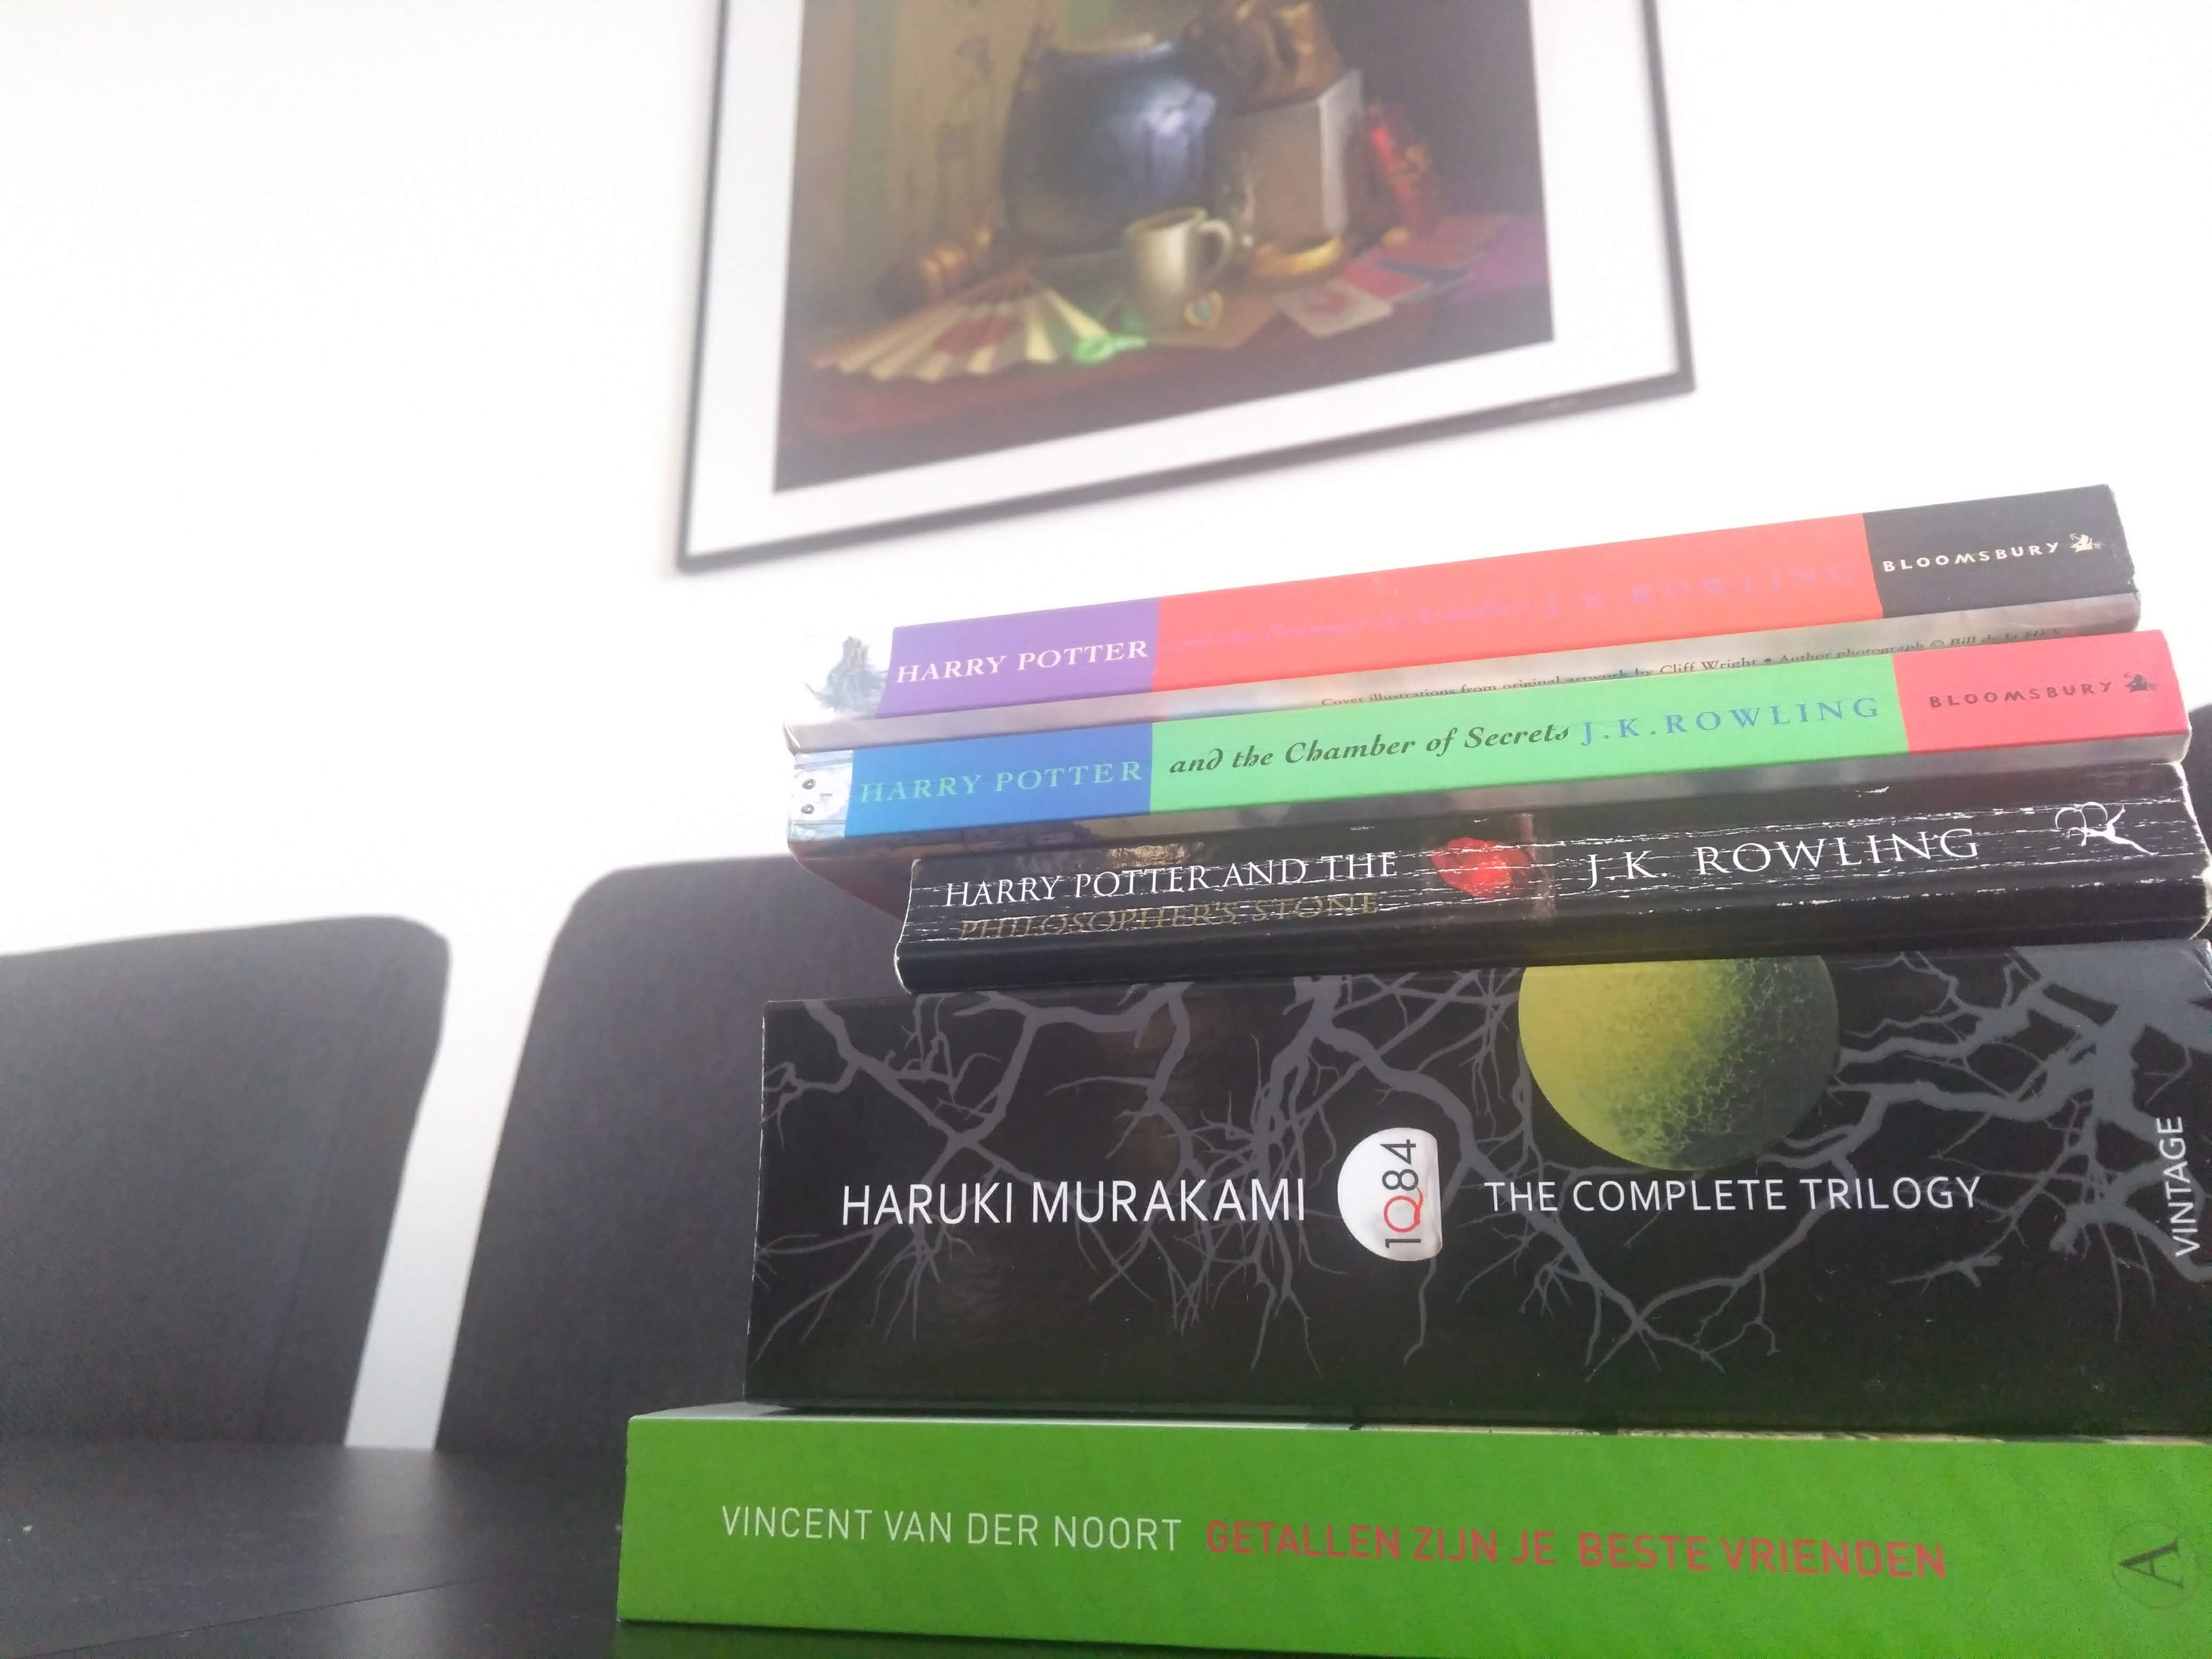
\includegraphics[width=\textwidth]{images/stack_read.jpg}\\
					}{
					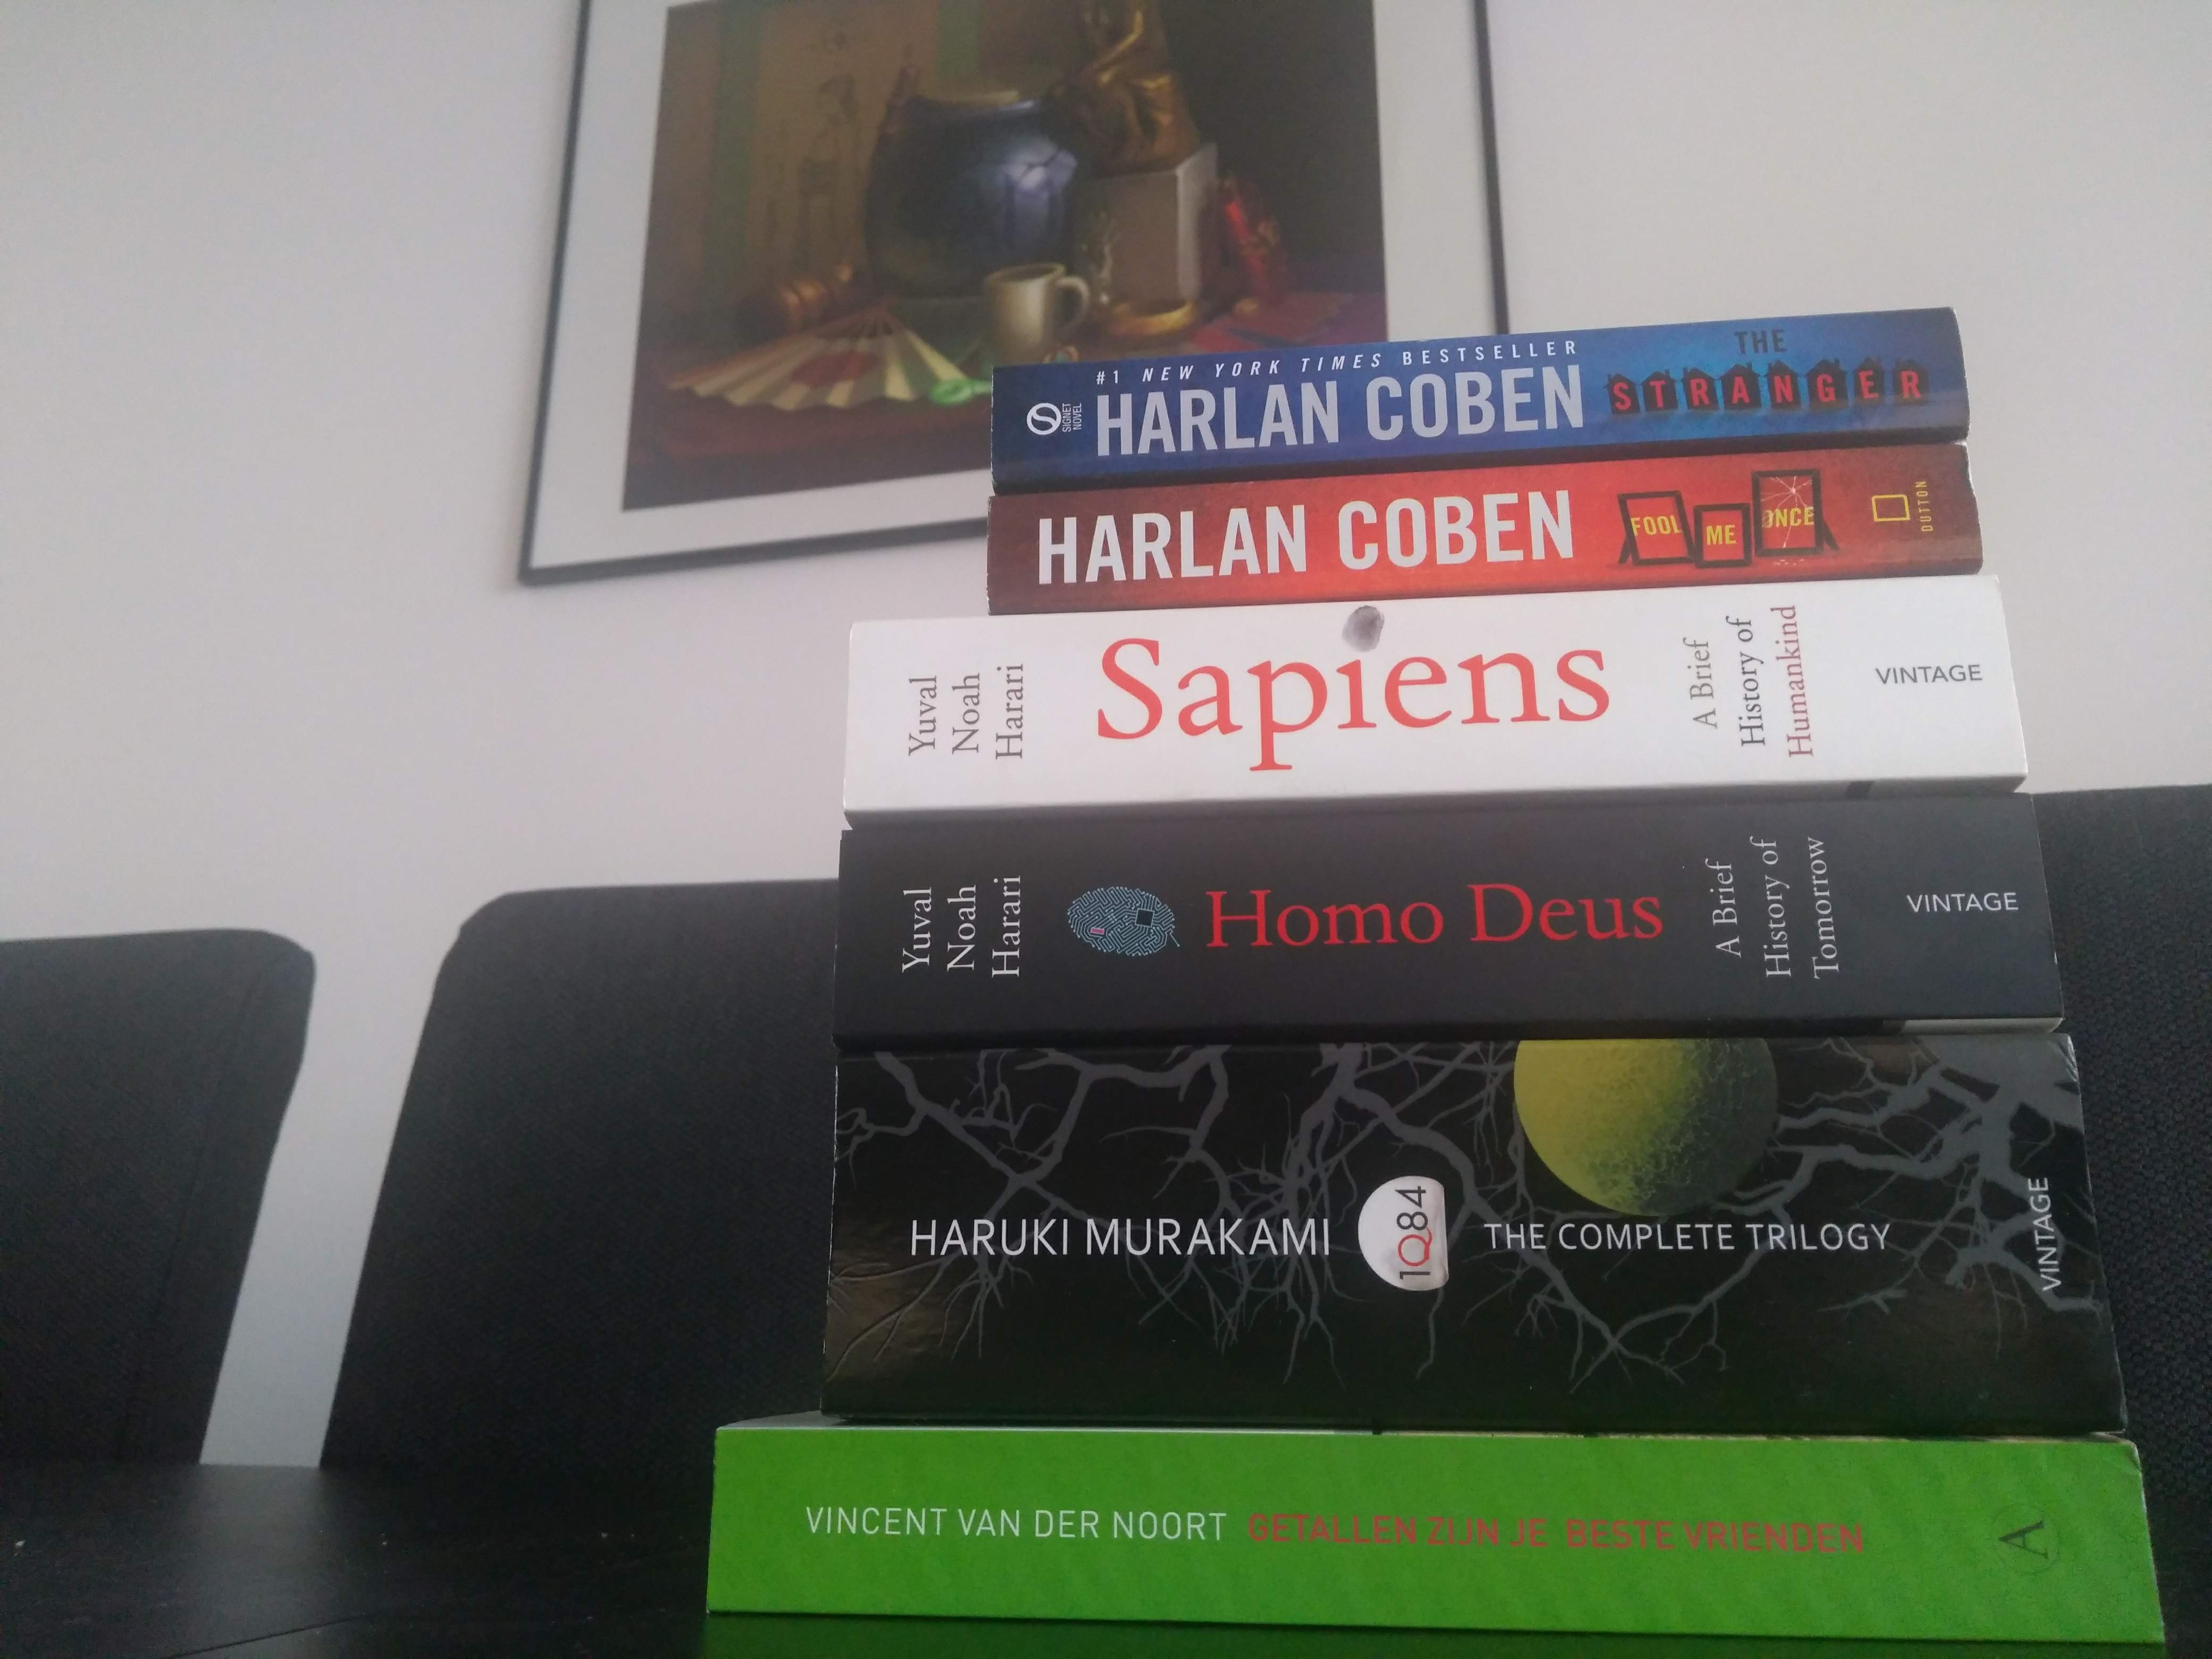
\includegraphics[width=\textwidth]{images/stack_unread.jpg}\\
					}
				\hspace*{15pt}\hbox{\scriptsize Image By:\thinspace{\itshape Stefan Hugtenburg}}
				\hspace*{15pt}\hbox{\scriptsize Bookcovers and picture in the back by others}
			\end{center}
		\column{0.455\textwidth}
		\begin{itemize}
			\item This is how I used to store books I still wanted to read.
				\pause
			\item A nice \alert{stack} of books, with new ones going on the top.
				\pause
			\item After finishing one, I would take the next one from the top.
				\pause
			\item So after a few weeks\dots
				\pause
			\item This uses the \alert{LIFO}-principle.
		\end{itemize}
	\end{columns}
\end{frame}

\begin{frame}
	\frametitle{The what!?}
	\framesubtitle{LIFO}
	
		\begin{block}{LIFO}
			The \textit{Last-In-First-Out}, or LIFO, principle is the working of a stack.\\
			\pause
			The last thing we've added to the stack is the first thing we take out.\\
			\pause
			Similarly the first we have added to the stack, is the last to be taken out.
		\end{block}	
\end{frame}

\begin{frame}
	\frametitle{The Stack ADT}
	\begin{overlayarea}{\textwidth}{\textheight}
		\only<1>{
			\begin{block}{ADT}
				An ADT, or Abstract Data Type, is a description of the behaviour of a data structure.
			\end{block}	
		}
		\pause
			\begin{block}{The Stack}
				\begin{itemize}
					\item \texttt{size()} (or \texttt{len(s)}) to get the number of items in the stack.
					\item \texttt{push(item)} to add something to the stack.
						\pause
					\item \texttt{pop()} to remove the top element from the stack.
					\item \texttt{top()} to view the top element of the stack.
				\end{itemize}
			\end{block}	
			\pause
			\begin{block}{Data structure?}
				What kind of data structure should we use to implement a Stack?
				\only<4>{
				\begin{enumerate}[A.]
					\item An array
					\item A python list
					\item A linked list
					\item A dict
				\end{enumerate}
			}
			\end{block}
			\pause
			\begin{block}{One end only}
				Only removing and adding on one end? Seems like a DLL will do.
			\end{block}
	\end{overlayarea}
\end{frame}

\begin{frame}
	\frametitle{Implementing a Linked-List based Stack}
	\begin{overlayarea}{\textwidth}{\textheight}
			\begin{tabular}{r | c c}
				Stack operation & DLL operation & Time Complexity \\
				\midrule
				\texttt{size} & \only<2->{\texttt{size} & $O(1)$} \\
				\texttt{push} & \only<2->{\texttt{add\_last} & $O(1)$} \\
				\texttt{pop}  & \only<2->{\texttt{remove\_last} & $O(1)$} \\
				\texttt{top}  & \only<2->{\texttt{tail} & $O(1)$} \\
			\end{tabular}
		
			\begin{columns}[t]
				\column{0.455\textwidth}
			\only<3->{
			\begin{block}{Arrays}
				Could we also do this using an array-based list?	
			\end{block}
		}
			\only<5->{
			\begin{block}{SLL}
				What about an SLL?
			\end{block}
		}
				\column{0.455\textwidth}
				\only<4->{
				\begin{block}{Amortised}
					Sure, but it's only amortised $O(1)$. So why would we?
				\end{block}
				}
				\only<6->{
				\begin{block}{Front = Back}
					Sure, but we add and remove from the front!
				\end{block}
				}
		
			\end{columns}
	\end{overlayarea}
\end{frame}

%%%%%%%%%%%%%%%%%%%%%%%%%%%%%%%%%%%%%%%%%%%%%%%%%%%%%%%%%%%%%%%%%%%%%%
\begin{frame}[fragile]\frametitle{}
\begin{center}
{\Large Maps}
\end{center}

\end{frame}


\begin{frame}
	\frametitle{Maps}
	
	\begin{center}
		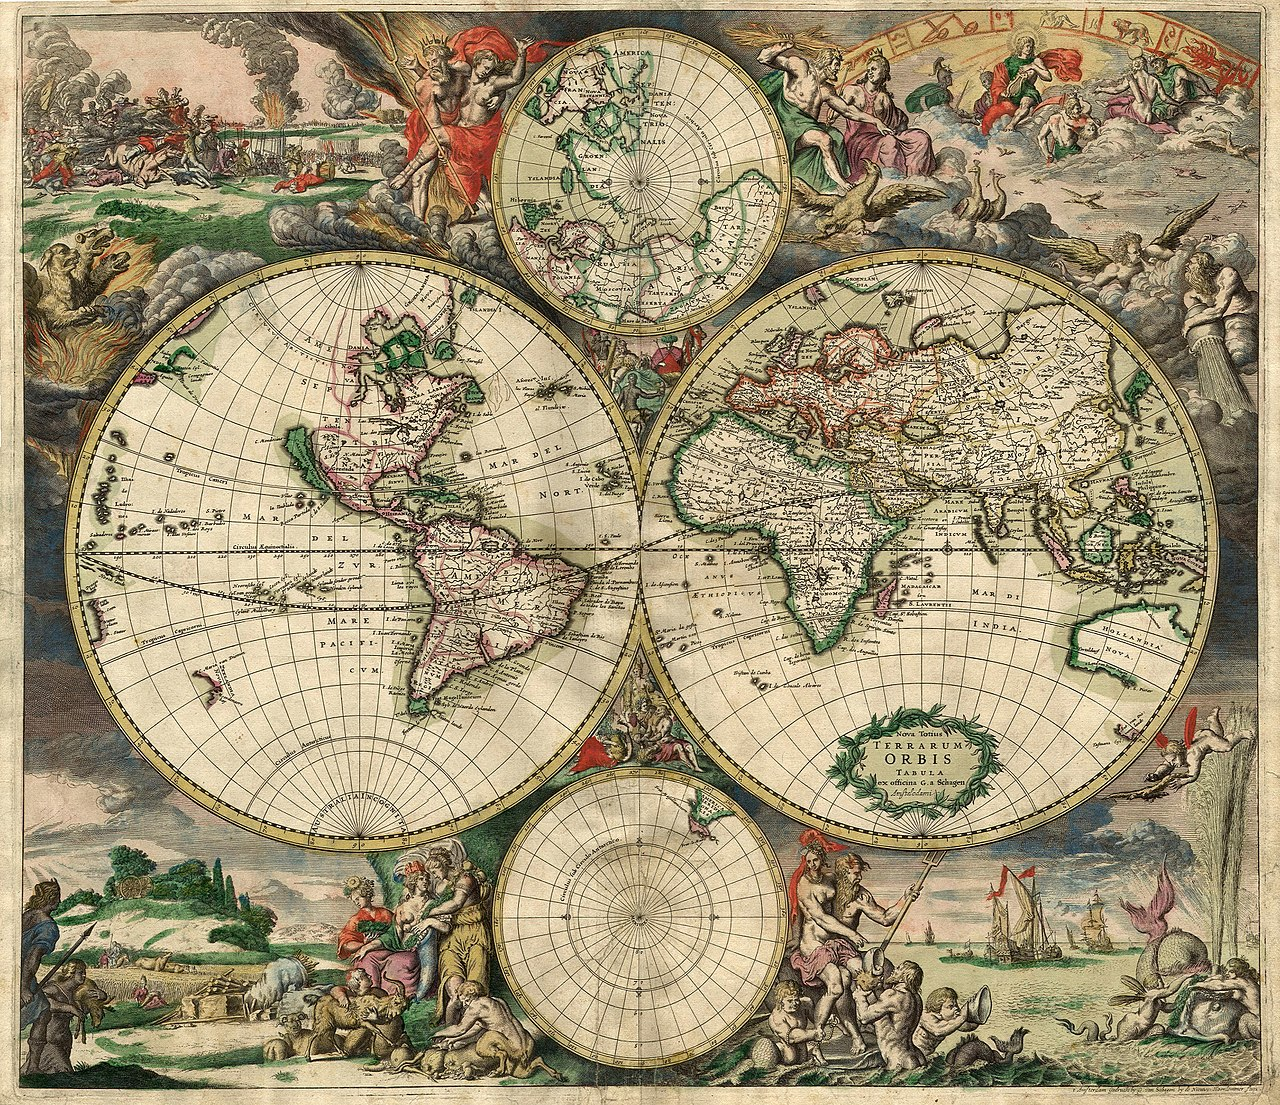
\includegraphics[width=0.5\textwidth]{images/world_map.JPG}\\
		\hspace*{15pt}\hbox{\scriptsize Image By:\thinspace{\itshape Gerard van Schagen}}
		%https://commons.wikimedia.org/wiki/File:World_Map_1689.JPG
	\end{center}
\end{frame}

\begin{frame}
	\frametitle{The map ADT}
	
		\begin{block}{The map ADT}
			Maps work on \textit{key-value} pairs, usually denoted as tuples: $(k,v)$.
			\pause
			\begin{itemize}
				\item \texttt{M.size()} (or \texttt{len(M)}) to get the number of tuples in the map.
					\pause
				\item \texttt{M.get(k)} (or \texttt{M[k]}) to retrieve the value for key $k$.
				\item \texttt{M.put(k,v)} (or \texttt{M[k] = v}) to set the value for key $k$ to $v$.
					\pause
				\item \texttt{M.remove(k)} (or \texttt{del M[k]}) to remove the tuple with key $k$.
					\pause
				\item \texttt{M.contains(k)} (or \texttt{k in M}) to determine if there is tuple with key $k$.
			\end{itemize}
		\end{block}	
\end{frame}

\begin{frame}
	\frametitle{A naive implementation}
	\framesubtitle{Listing a map}

	\begin{block}{Why not just use a list?}
		If we use a list to implement the map where we just throw in all the tuples, what would the time complexity
		of the functions \texttt{get}, \texttt{remove}, \texttt{contains} be?
		\pause
		\begin{enumerate}[A.]
			\item $\Theta(1)$
			\item $\Theta(\log n)$
			\item $\Theta(n)$
			\item $\Theta(n^2)$
			\item I don't know
		\end{enumerate}
	\end{block}
	\pause
	\begin{block}{Not so great}
		All would take linear time! \\
		We would just have to check all the objects every time!
	\end{block}
\end{frame}

\begin{frame}
	\frametitle{Can we do better?}
	\begin{block}{Can we do better?} 
		Can we do better, and if so how?
	\end{block}	
	\pause
	\begin{block}{Yes!}
		How about we try to use an array-based structure where the key determines the index?\\
		\pause
		This allows for $\Theta(1)$ operations for getting, removing or checking an item!
	\end{block}
	\pause
	\begin{block}{But...}
		But what if the key is not integer?
	\end{block}
\end{frame}


\begin{frame}
	\frametitle{A hash}
\begin{center}
	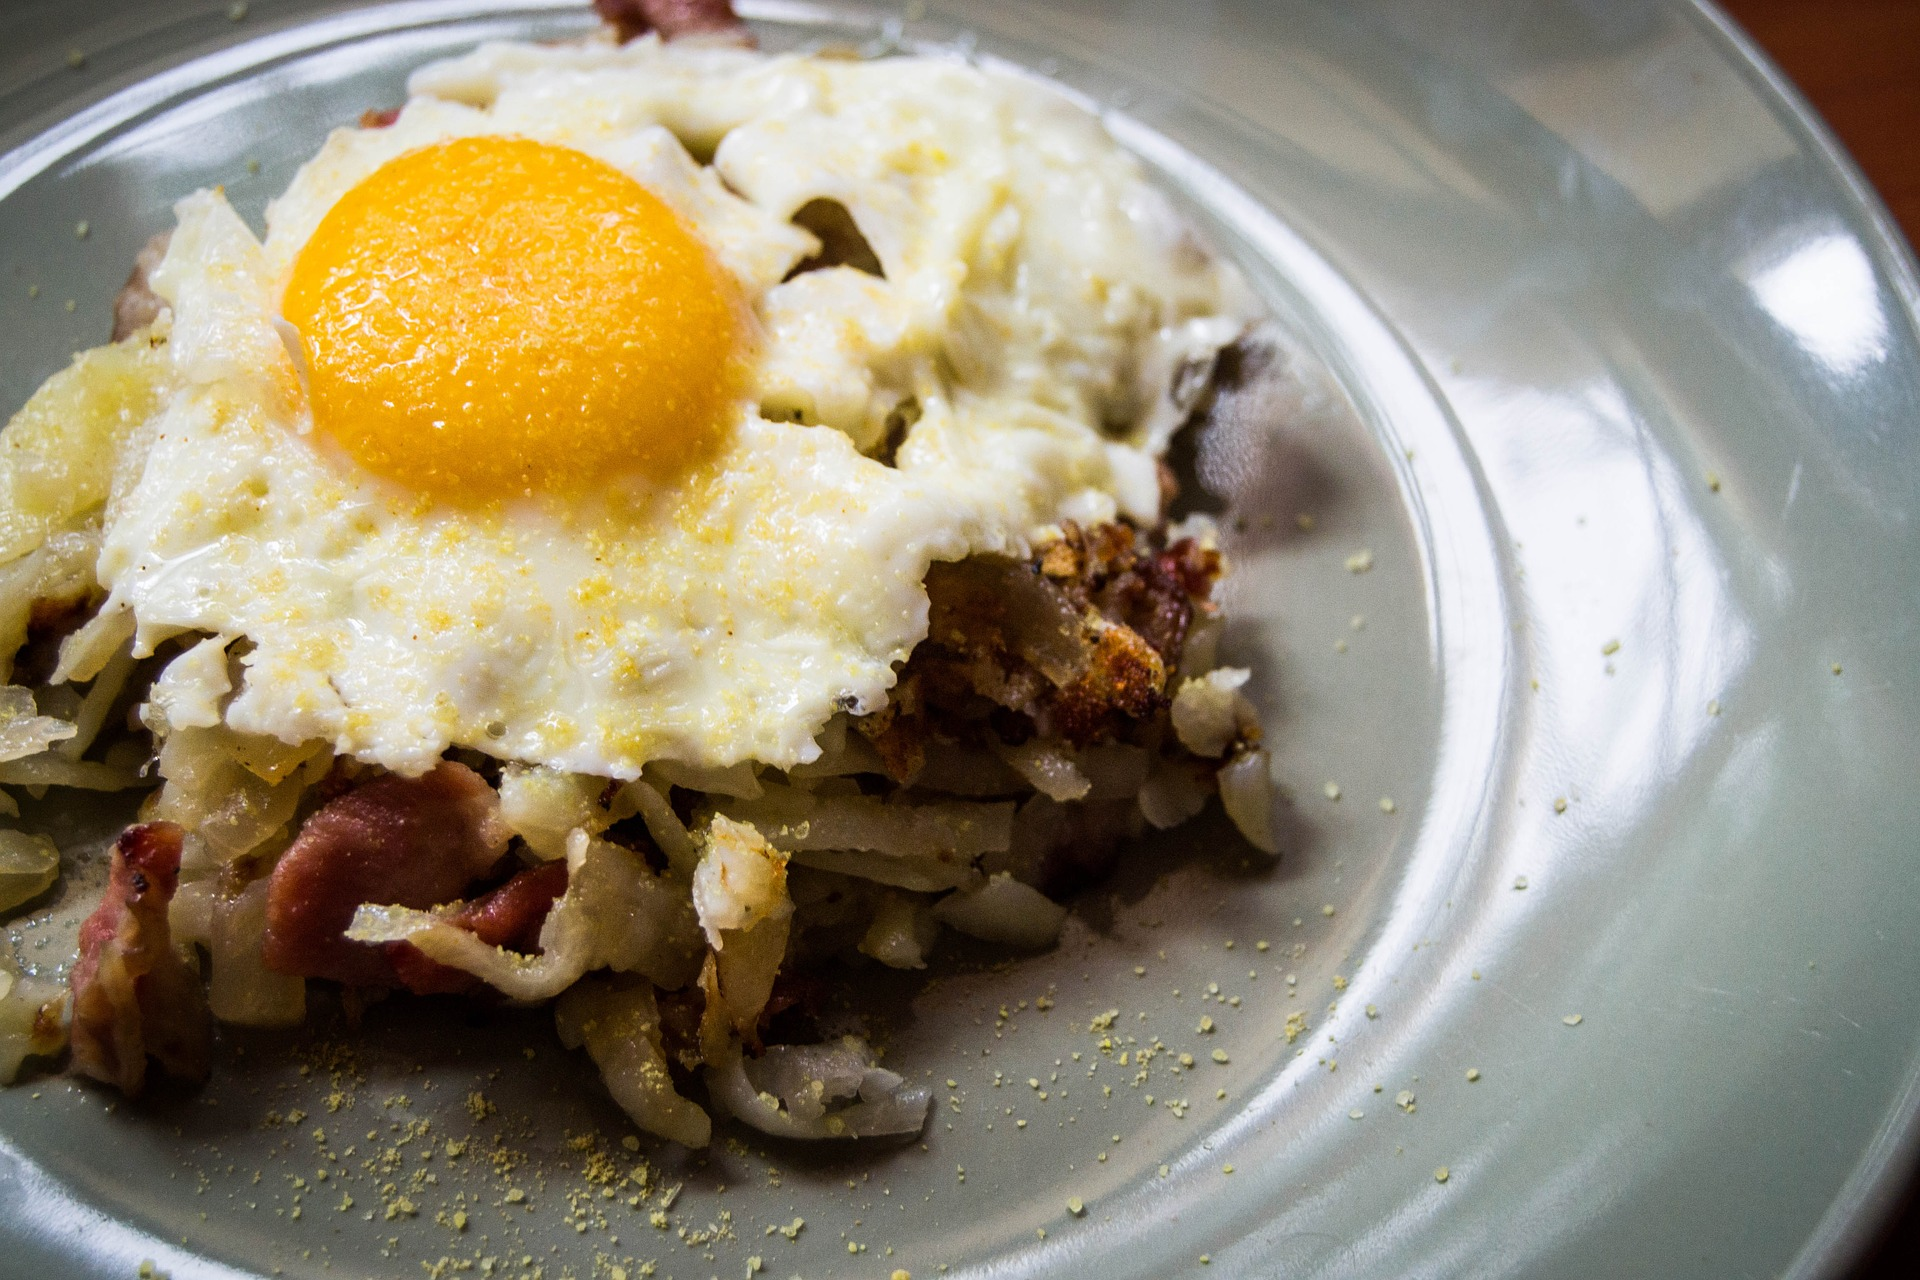
\includegraphics[width=0.6\textwidth]{images/hash.jpg}\\
	\hspace*{15pt}\hbox{\scriptsize Image By:\thinspace{\itshape ailinder}}
	% https://pixabay.com/photos/hash-eggs-food-meal-potato-plate-1330575/
\end{center}
\end{frame}

\begin{frame}
	\frametitle{Hash functions}
	
		\begin{block}{Hash functions}
			Hash functions map each key $k$ to a an integer in a range $[0, N-1]$ for some $N$.\\
		\end{block}	
		\pause
		\begin{block}{That's easy right?}
			Consider the hash function $f(k) = 1$ for any key $k$.\\
			Is this a hash function for $N=100$?
			\begin{enumerate}[A.]
				\item Yes
				\item No
				\item I don't know
			\end{enumerate}
		\end{block}

		\pause
			\begin{block}{It is...}
				It is a hash function, but a terrible one!\\
				Why?
			\end{block}	
\end{frame}

\begin{frame}
	\frametitle{Hash to determine the index}

	\begin{block}{A hash table}
		We want to use hash functions to map keys to a certain index in a hash table.
	\end{block}
	\pause
	\begin{block}{Back to hundred-acre woods}
		Take $f(p) = 1$, $f(i) = 3$, $f(g) = 2$, $f(l) = 8$, $f(e) = 5$, $f(t) = 7$.
		\pause
		This would create the hash table:
		\begin{center}
			\begin{tikzpicture}[scale=0.85, transform shape]
	\foreach \x/\val in {0/,1/p,2/g,3/i,4/,5/e,6/,7/t,8/l,9/,10/}{
	\node[olive] (index) at (\x,1) {\x};
	\node[draw,rectangle, fill=gray!10, minimum size =1cm] (c) at (\x,0) {\val};
}
\node[] at (-2,1) {Indices:};
\node[] at (-2,0) {Array:};
\end{tikzpicture}

		\end{center}
	\end{block}	
	\pause
	\begin{block}{The simple mapping}
		But what if we have conflicts? Like by taking $f(k)=1$ for all $k$.
	\end{block}	
\end{frame}

\begin{frame}
	\frametitle{Hashing conflicts}
	\begin{block}{A hash table}
		We want to use hash functions to map keys to a certain index in a hash table.\\
		But what do we do if we have hashing conflicts?
	\end{block}
	\pause
	\begin{block}{Back to hundred-acre woods}
		Take $f(e) = 1$, $f(y) = 3$, $f(o) = \alert{3}$, $f(r) = 8$.
		\pause
		This would create the hash table:
		% \begin{center}
			% \begin{tikzpicture}[scale=0.85, transform shape]
	\foreach \x/\val in {0/,1/,2/,3/,4/,5/,6/,7/,8/,9/,10/}{
	\node[olive] (index) at (\x,1) {\x};
	\node[draw,rectangle, fill=gray!10, minimum size =1cm] (\x) at (\x,0) {\val};
}
\node[] at (-2,1) {Indices:};
\node[] at (-2,0) {Array:};

\node[draw,rectangle, fill=gray!10, minimum size =0.5cm] at (1,-1.5) (e) {e};
\node[draw,rectangle, fill=gray!10, minimum size =0.5cm] at (3,-1.5) (A) {y};
\node[draw,rectangle, fill=gray!10, minimum size =0.5cm] at (3,-2.5) (B){o};
\node[draw,rectangle, fill=gray!10, minimum size =0.5cm] at (8,-1.5) (r) {r};
\draw[->, ultra thick] (A) -- (B);
\draw[*->, ultra thick] (1.center) -- (e);
\draw[*->, ultra thick] (3.center) -- (A);
\draw[*->, ultra thick] (8.center) -- (r);
\end{tikzpicture}

		% \end{center}
	\end{block}	
\end{frame}

\begin{frame}
	\frametitle{Hash tables}
	\begin{block}{Hash tables}
		We have an array of a certain capacity.\\
		The hash of a key, determines which \textit{bucket} to use.\\
		\pause
		Every entry could for instance hold a linked-list of values.
	\end{block}		
	\pause
	\begin{columns}
		\column{0.455\textwidth}
			
	\begin{block}{What happens?}
		So for $f(k) = 1$ for all $k$, what is the time complexity of getting the right value out for our key?
		\begin{enumerate}[A.]
			\item $\Theta(1)$
			\item $\Theta(\log n)$
			\item $\Theta(n)$
			\item $\Theta(n^2)$
		\end{enumerate}
	\end{block}
		\column{0.455\textwidth}
			
		\pause
		\begin{block}{Still linear}
			It is still linear time! All end up in a list after all.
		\end{block}
	\end{columns}
\end{frame}

\begin{frame}
	\frametitle{Hash functions: Ideal properties}
	
		\begin{block}{Hash functions}
			Hash functions map each key $k$ to a an integer in a range $[0, N-1]$ for some $N$.\\
			Where ideally:
			\pause
			\begin{itemize}
				\item keys are uniformly distributed over the range.
					\pause
				\item ($a == b) \to (\mathit{hash}(a) == \mathit{hash}(b))$ (it is deterministic).
					\pause
				\item the hash function is `fast' to compute (preferably $O(1)$).
			\end{itemize}

		\end{block}	
			\begin{block}{Rotten to the core}
				This indeed makes $f(k) = 1$ pretty terrible!
			\end{block}	
\end{frame}

\begin{frame}
	\frametitle{Implementing them in Python}
	\only<4->{\framesubtitle{Check for yourself, write a bit of code to count conflicts!}}
		\vspace{-10pt}
	\begin{columns}
		\column{0.555\textwidth}
			\lstinputlisting{src/point.py}
		\pause
		\column{0.555\textwidth}
		\lstinputlisting[firstline=4, lastline=15]{src/point2.py}
	\end{columns}
	\pause
		\vspace{-10pt}
	\begin{block}{Does it improve?}
		Which is better?	
		\vspace{-10pt}
		% \begin{multicols}{3}
		\begin{enumerate}[A.]
			\item The left one.
			\item The right one.
			\item I don't know.
		\end{enumerate}
	% \end{multicols}
	\end{block}
	\pause
		\vspace{-8pt}
		\begin{block}{It depends!}
			It depends on what kind of points we expect to see!
		\end{block}
\end{frame}


\begin{frame}
	\frametitle{Hashmaps}
	\framesubtitle{Have fun figuring out what this map represents.}
	\begin{center}
		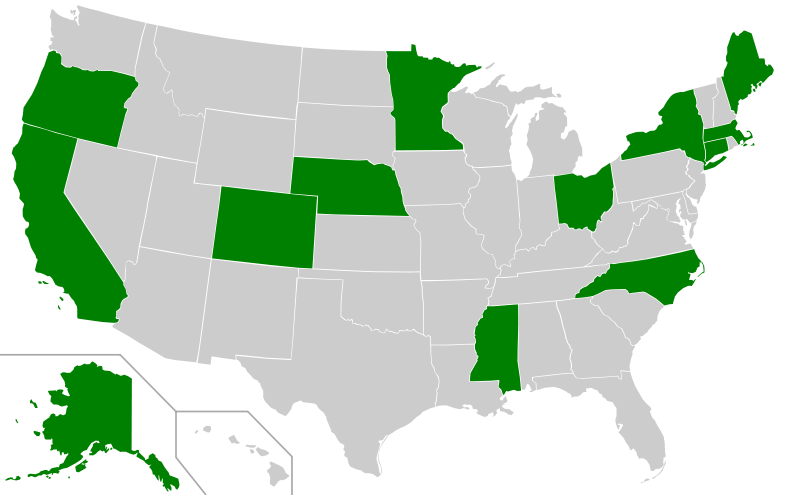
\includegraphics[width=0.6\textwidth]{images/hashmap.png}\\
		\hspace*{15pt}\hbox{\scriptsize Image By:\thinspace{\itshape Photohound}}
	\end{center}
\end{frame}

\begin{frame}
	\frametitle{Hashmaps}
		\begin{block}{Hashmaps}
			Implement the Map ADT using Hash tables.\\
			\pause
			With a good hash function, we expect: $\Theta(1)$ insertion/deletion/retrieval.\\
			But worst-case they are still $\Theta(n)$.
		\end{block}	
		\pause
		\begin{block}{Handling hashing conflicts}
			Different options to handle hash conflicts:
			\begin{itemize}
				\item Separate Chaining
				\item (Linear) Probing
			\end{itemize}
		\end{block}
\end{frame}

\begin{frame}
	\frametitle{Lets start with the basics}
	\vspace{-13pt}
	\begin{columns}
		\column{0.355\textwidth}
		\begin{itemize}
			\item Creating a new hashmap
			\item<2-> Getting the size
			\item<3-> A hash function for keys in this map
			\item<4-> Getting an item
			\item<4-> Putting an item
		\end{itemize}
		\column{0.555\textwidth}
			
		\lstinputlisting[basicstyle=\tiny\ttfamily
		% ,linebackgroundcolor={%
			% \btLstHL<1>{3-5}%
			% \btLstHL<2>{7-8}%
			% \btLstHL<3>{10-11}%
			% \btLstHL<4>{13-15}%
			% \btLstHL<5>{17-21}%
		% }
		]
		{src/hashmap.py}
	\end{columns}
	\only<5->{
			\begin{block}{So conclusion}
				It depends on how we put things into the buckets!\\
				Do we use the linked list? Or do we do something else?
			\end{block}	
	}
\end{frame}


\begin{frame}
	\frametitle{Recap of Maps}
	
	\begin{center}
		\begin{tabular}{c | c | c}
			Operation & Expected Time & Worst-case \\
			\midrule
			\texttt{M.size()} & $\Theta(1)$& $\Theta(1)$\\
			\texttt{M.get(k)}  & $\Theta(1)$& $\Theta(n)$\\
			\texttt{M.put(k,v)} & $\Theta(1)$& $\Theta(n)$\\
			\texttt{M.remove(k)} & $\Theta(1)$& $\Theta(n)$\\
			\texttt{M.contains(k)} & $\Theta(1)$& $\Theta(n)$\\
		\end{tabular}
	\end{center}
		\begin{block}{What does this depend on?}
			It all stands or falls with the hash function!
			\begin{itemize}
				\item Fewer hash-conflicts means better performance.
				\item Separate chaining or (linear) probing does not matter for time performance.
				\item The latter saves us some space, but is not better in terms of space or time \textit{complexity}.
			\end{itemize}
		\end{block}	
\end{frame}



%%%%%%%%%%%%%%%%%%%%%%%%%%%%%%%%%%%%%%%%%%%%%%%%%%%%%%%%%%%%%%%%%%%%%%
\begin{frame}[fragile]\frametitle{}
\begin{center}
{\Large Trees}
\end{center}

\end{frame}


\begin{frame}
	\frametitle{Binary Trees}
	\framesubtitle{Tikz taken from: \url{http://texample.net/tikz/examples/red-black-tree/}}
	\begin{center}
			\begin{tikzpicture}[level/.style={sibling distance = 4cm, %->,>=stealth',
		  level distance = 1.5cm},
			  treenode/.style = {align=center, inner sep=0pt, text centered,
		    font=\sffamily},
		  arn_n/.style = {treenode, circle, white, font=\sffamily\bfseries, draw=black,
		    fill=black, text width=1.5em},% arbre rouge noir, noeud noir
		  arn_r/.style = {treenode, circle, red, draw=red,
		    text width=1.5em, very thick},% arbre rouge noir, noeud rouge
		  arn_x/.style = {treenode, rectangle, draw=black,
		    minimum width=0.5em, minimum height=0.5em}% arbre rouge noir, nil
			]
			\node [arn_n] {33}
    child{ node [arn_r] {15}
            child{ node [arn_n] {10}
            	child{ node [arn_r] {5} edge from parent node[above left]
                         {$x$}} %for a named pointer
							child{ node [arn_x] {}}
            }
            child{ node [arn_n] {20}
							child{ node [arn_r] {18}}
							child{ node [arn_x] {}}
            }
    }
    child{ node [arn_r] {47}
            child{ node [arn_n] {38}
							child{ node [arn_r] {36}}
							child{ node [arn_r] {39}}
            }
            child{ node [arn_n] {51}
							child{ node [arn_r] {49}}
							child{ node [arn_x] {}}
            }
		}
;
\end{tikzpicture}
	\end{center}
	
\end{frame}

\begin{frame}
	\frametitle{Binary Trees}
	\framesubtitle{All we need}

		\begin{block}{Binary Trees}
			\begin{itemize}
				\item Every node has at most 2 children.
					\pause
				\item One \textit{left} child and one \textit{right} child.
			\end{itemize}
		\pause
		A binary tree is \textit{proper} or \textit{full} if all nodes have either 0 or 2 children.
		\end{block}	

		\pause
		\begin{columns}
			\column{0.455\textwidth}
				
			\begin{tikzpicture}[
				level distance = 2.5em,
				level 1/.style={sibling distance=9em},
				level 2/.style={sibling distance=4.5em},
				level 3/.style={sibling distance=2.25em},
			]
			\node[circle] (t1) {root}
				child { node[circle]   {child 1}
					child { node[circle] {l1}}
					child { node[circle] {l2}}
				}
				child { node[circle]   {child 2}
					child { node[circle] {l3}}
					child { node[circle] {l4}
						child { node[circle] {l5}}
						child { node[circle] {l6}}
					}
				};
			\end{tikzpicture}
			\column{0.455\textwidth}
				
			\begin{block}{Is it full?}
				Is this tree full?
				\begin{enumerate}[A.]
					\item Yes
					\item No
					\item I don't know
				\end{enumerate}
			\end{block}
		\end{columns}
\end{frame}

\begin{frame}
	\frametitle{All kinds of fun properties!}
	
		\begin{block}{Many interesting properties}
			There are many interesting relations in binary trees, between the number of internal nodes vs leaves, height, etc.	
		\end{block}	
		\pause
		\begin{block}{Just one example}
			There is always one more leaf than there are internal nodes in a full binary tree.
		\end{block}	
\end{frame}

\begin{frame}
	\frametitle{Tree properties pt2}
	\begin{center}
		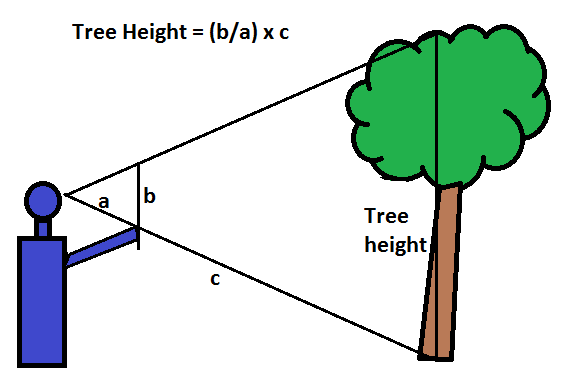
\includegraphics[width=0.6\textwidth]{images/stick.png}\\
		\hspace*{15pt}\hbox{\scriptsize Image By:\thinspace{\itshape Edfrank01}}
		% https://commons.wikimedia.org/wiki/File:Stick_measurement.png
	\end{center}
\end{frame}

\begin{frame}
	\frametitle{Depth of a node}

	\begin{columns}
		\column{0.405\textwidth}
			\begin{tikzpicture}[
				level distance = 2.5em,
				level 1/.style={sibling distance=9em},
				level 2/.style={sibling distance=4.5em},
				level 3/.style={sibling distance=2.25em},
			]
			\node[circle] (t1) {root}
				child { node[circle]   {child 1}
					child { node[circle] {l1}}
				}
				child { node[circle]   {child 2}
					child { node[circle] {l2}}
					child { node[circle] {l3}}
					child { node[circle] {l4}}
				};
			\end{tikzpicture}
		\column{0.555\textwidth}
		\begin{itemize}
			\item The \textit{depth} of a \alert<5->{node} is the distance to the root.
				\pause
			\item So depth(root) = 0.
			\item And depth(l2) = 2.
				\pause
			\item The \textit{height} of a \alert<5->{tree} is the length of the longest path from root to leaf.
				\pause
			\item So the height of this tree is 3.
				\pause
			\item Note: Every book/author has their own definition of these things! Including our book :(
		\end{itemize}
	\end{columns}
	
\end{frame}

\begin{frame}
	\frametitle{Depth of a node}

	\begin{columns}
		\column{0.405\textwidth}
			\begin{tikzpicture}[
				level distance = 2.5em,
				level 1/.style={sibling distance=9em},
				level 2/.style={sibling distance=4.5em},
				level 3/.style={sibling distance=2.25em},
			]
			\node[circle] (t1) {root}
				child { node[circle]   {child 1}
					child { node[circle] {l1}}
				}
				child { node[circle]   {child 2}
					child { node[circle] {l2}}
					child { node[circle] {l3}}
					child { node[circle] {l4}}
				};
			\end{tikzpicture}
		\column{0.555\textwidth}
		\begin{block}{Alternative definition for height}
			How can we also describe the tree height of a tree $T$?
			\pause
			\begin{enumerate}[A.]
				\item $\max\limits_{v\in T}({\textit{depth}(v)})-1$
				\item $\max\limits_{v\in T}({\textit{depth}(v)})$
				\item $\max\limits_{v\in T}({\textit{depth}(v)})+1$
			\end{enumerate}
		\end{block}
	\end{columns}
	\pause
	\begin{block}{A tree of height one}
		Remember that a tree of height one is just the root, which is at depth $0$. So it cannot be A or B.\\
		Then remember that depth is the distance, but height is the length of the path. These differ by 1, so C is the right
		answer.\\
		Our book uses $B$ :( 
	\end{block}
\end{frame}

\begin{frame}
	\frametitle{An implementation}
	
	\begin{block}{How do we implement this?}
		How can we implement such a tree structure?
	\end{block}
	\pause
	\begin{block}{Just like a DLL, only different}
		By using nodes that are \textit{linked} together to form a tree!
	\end{block}
	\pause
	\begin{columns}[t]
		\column{0.535\textwidth}
	\lstinputlisting{src/tree.py}
			
		\column{0.505\textwidth}
	\lstinputlisting{src/treenode.py}
			
	\end{columns}
\end{frame}

\begin{frame}
	\frametitle{Now we can create functions!}
	\begin{block}{Implementing functionality}
		What kind of \textit{programming paradigm} will we use to implement tree functions?
	\end{block}
	\pause
	\begin{block}{See the contents of this box}
		See the title of this box.
	\end{block}
\end{frame}

\begin{frame}
	\frametitle{Node Depth}
		\begin{block}{Example: Node depth}
			Find the depth of a node is easy if we know the depth of the parent.
		\end{block}	
		\pause
		\lstinputlisting{src/nodedepth.py}
\end{frame}

\begin{frame}
	\frametitle{Tree Height}
		\begin{block}{Example: Tree height}
			The height of the tree is the max depth + 1! 	
		\end{block}	
		\pause
		\lstinputlisting{src/treeheight.py}
\end{frame}

\begin{frame}
	\frametitle{Getting all the leaves}
	\begin{block}{It's autumn time}
		How can we get all the leaves from a tree?
	\end{block}
		\pause
		\lstinputlisting{src/treeleaves.py}
\end{frame}

\begin{frame}
	\frametitle{The full ADT}
		\begin{block}{A Tree ADT}
			Different implementations of trees, give you different ADTs.\\
			The book uses one which is \textit{position}-focused.\\
			The properties are always the same, just the functions and how to call them can be different.
		\end{block}	
\end{frame}

\begin{frame}
	\frametitle{Alternative implementation}
		\begin{block}{An observation}
			Every node in a tree, is the root to a subtree!
		\end{block}	
		\pause
		\begin{columns}
			\column{0.455\textwidth}
				
			\begin{tikzpicture}[
				level distance = 2.5em,
				level 1/.style={sibling distance=9em},
				level 2/.style={sibling distance=4.5em},
				level 3/.style={sibling distance=2.25em},
			]
			\node[circle] (t1) {root}
				child { node[circle]   {child 1}
					child { node[circle] {l1}}
				}
				child { node[circle]   {child 2} % ,
					child { node[circle] {\alert<3>{l2}}}
					child { node[circle] {\alert<3>{l3}}}
					child { node[circle] {\alert<3>{l4}}
						child { node[circle] {\alert<3>{l5}}}
						child { node[circle] {\alert<3>{l6}}}
					}
				};
			\end{tikzpicture}
			\pause
			\column{0.455\textwidth}
				\begin{block}{A subtree}
					In the example on the right, child 2 is the root of the subtree drawn in red.
				\end{block}	
		\end{columns}
\end{frame}

\begin{frame}
	\frametitle{Alternative implementation}
		\begin{block}{Thinking of all nodes as trees}
			By implementing it like this, we have no need for \texttt{TreeNode}s. All nodes are just \texttt{Tree}s!
		\end{block}	

		\lstinputlisting{src/tree_alt.py}
\end{frame}

\begin{frame}
	\frametitle{Alternative implementation: Tree Height}
	\begin{block}{What do we do?}
		How do we determine the height in this set-up?
	\end{block}
	\pause
	\lstinputlisting{src/tree_alt_height.py}
\end{frame}

\begin{frame}
	\frametitle{Why have one implementation over the other?}

	\begin{block}{Which is better?}
		Which implementation should you use?
	\end{block}
	\pause
	\begin{block}{IT DEEP ENDS}
		It depends of course ;)\\
		What information do you need to store for your use case?
	\end{block}
	
\end{frame}



\begin{frame}
	\frametitle{Tree time}
	\begin{center}
		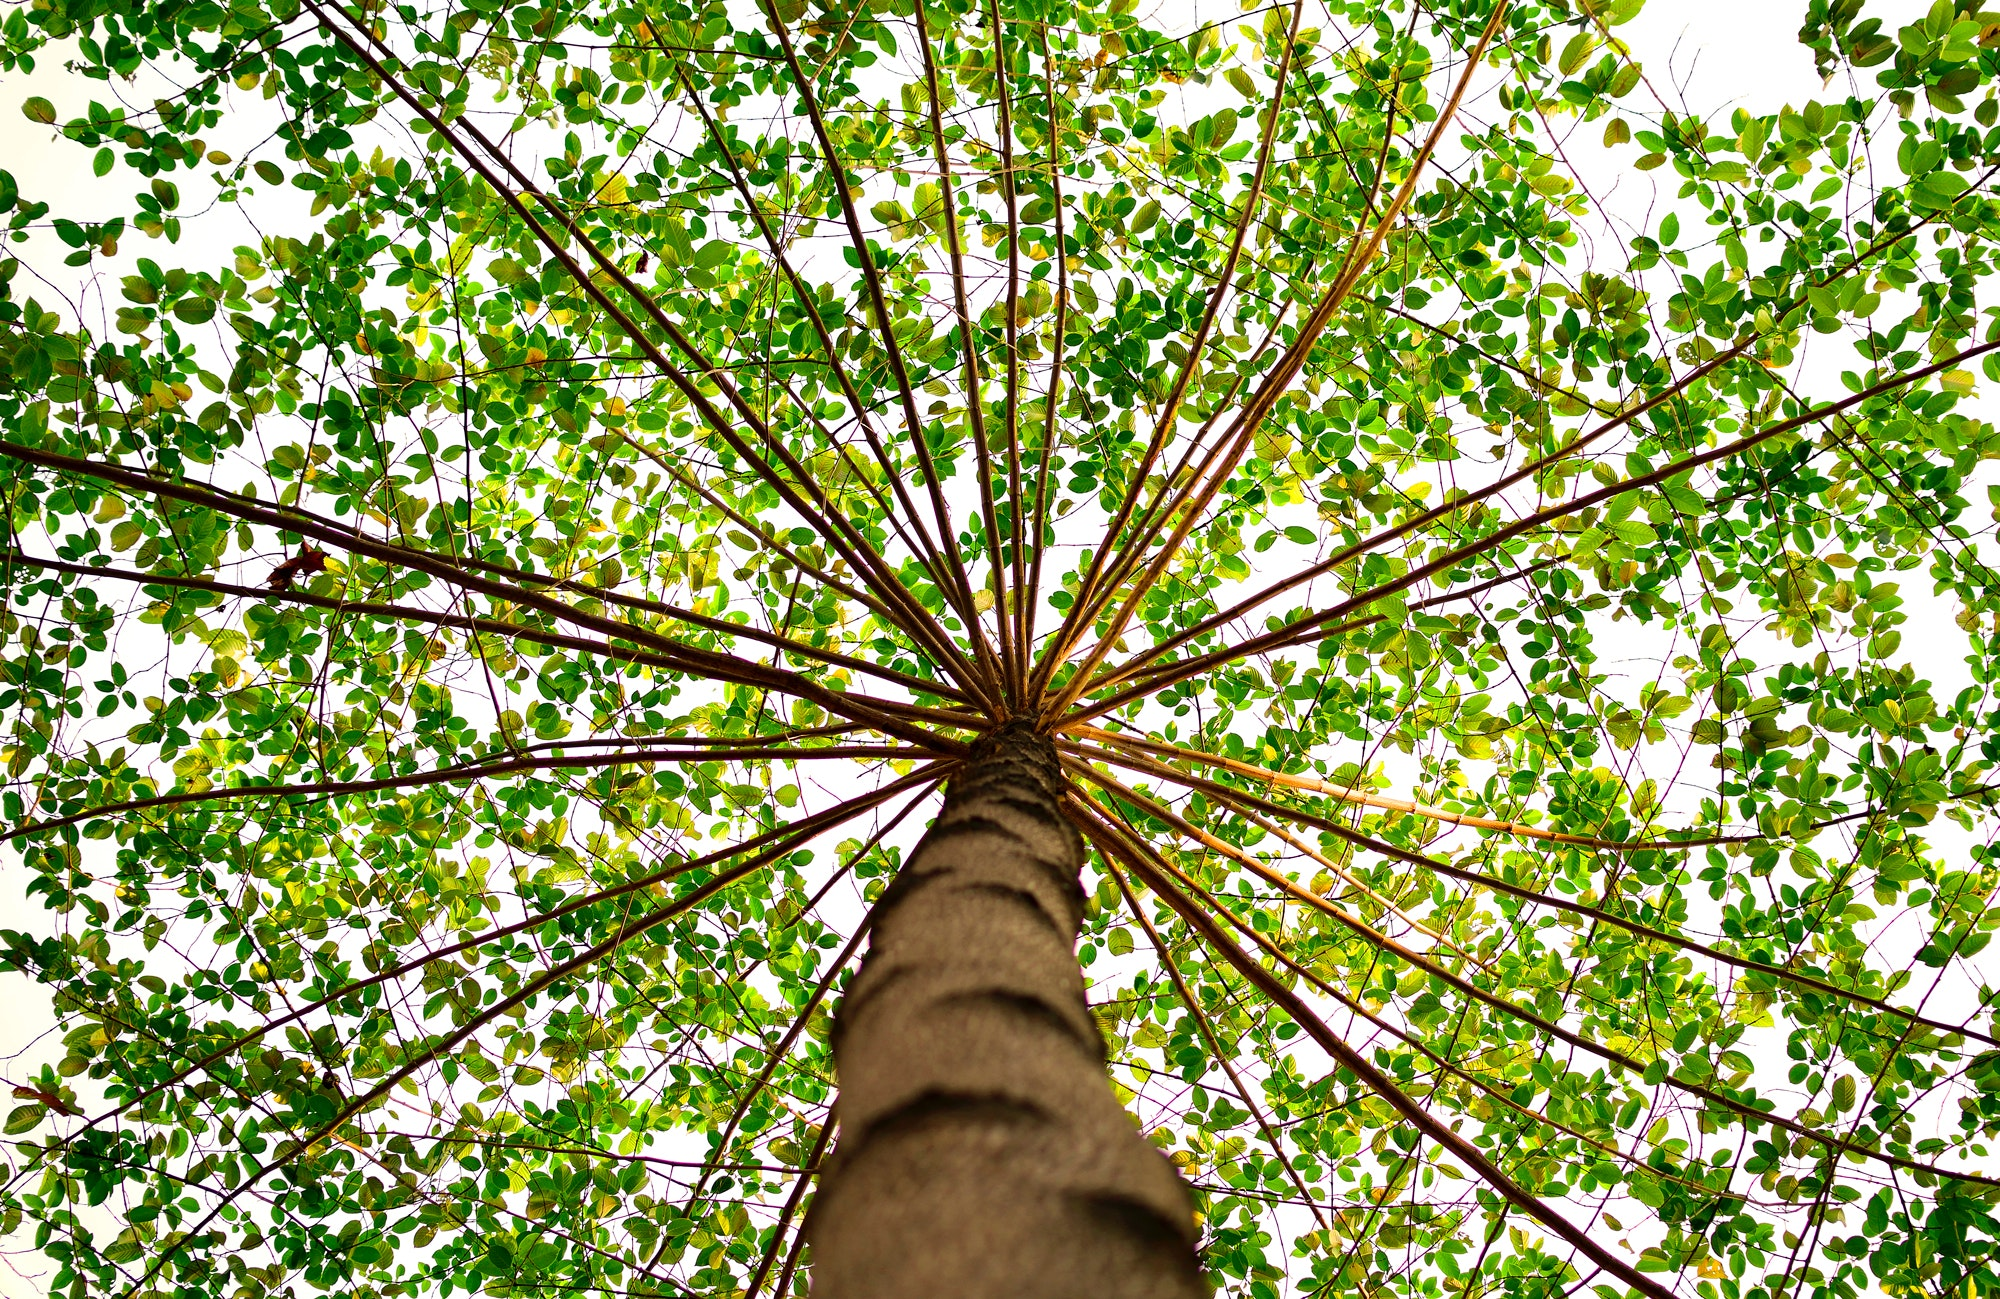
\includegraphics[width=0.6\textwidth]{images/tree.jpg}\\
		\hspace*{15pt}\hbox{\scriptsize Image By:\thinspace{\itshape George achik}}
		% https://commons.wikimedia.org/wiki/File:Last_summer_time_tree_and_evening_time,_In_Srimongol,_Bangladesh.jpg
	\end{center}
\end{frame}

\begin{frame}
	\frametitle{Properties}
	\begin{columns}
		\column{0.405\textwidth}
			\begin{tikzpicture}[
				level distance = 2.5em,
				level 1/.style={sibling distance=9em},
				level 2/.style={sibling distance=4.5em},
				level 3/.style={sibling distance=2.25em},
			]
			\node[circle] (t1) {\alert<1,6>{root}} % ,onslide=<5>{draw=red}
				child { node[circle] {\alert<2,4,5>{child 1}}
					child { node[circle] {\alert<3,5>{leaf 1}}}
				}
				child { node[circle] {\alert<2,4,5,6>{child 2}}
					child { node[circle] {\alert<3,5>{leaf 2}}}
					child { node[circle] {\alert<3,5>{leaf 3}}}
					child { node[circle] {\alert<3,5>{leaf 4}}}
				};
			\end{tikzpicture}
		\column{0.555\textwidth}
		\begin{itemize}
			\item The \textit{root node} is the node that has no \textit{parent}.
				\pause
			\item A node can have \textit{children}.
				\pause
			\item A node without children is called a \textit{leaf}.
				\pause
			\item Two nodes with the same \textit{parent} are \textit{siblings}.
				\pause
			\item \textit{Descendants} are found by repeatedly following child-relations.
				\pause
			\item \textit{Ancestors} are found by repeatedly following parent-relations.
		\end{itemize}
	\end{columns}
\end{frame}

\begin{frame}
	\frametitle{Quick check}
	
	\begin{columns}
		\column{0.405\textwidth}
			\begin{tikzpicture}[
				level distance = 2.5em,
				level 1/.style={sibling distance=2em},
				level 2/.style={sibling distance=4.5em},
				level 3/.style={sibling distance=2.25em},
			]
			\node[circle] (t1) {r}
				child { node[circle] {k}
					child { node[circle] {d}}
				}
				child { node[circle] {a} }
				child { node[circle] {b} }
				child { node[circle] {e} 
					child { node[circle] {g} }
					child { node[circle] {h}
						child { node[circle] {i}}
					}
				}
				child { node[circle] {f} };
			\end{tikzpicture}
		\column{0.555\textwidth}
		\pause
			\begin{block}{Let's see if that was a clear}
				Let $c(v)$ be the set of children of $v$.\\
				Let $d(v)$ be the set of descendants of $v$.\\
				Let $s(v)$ be the set of siblings of $v$.\\
				Let $a(v)$ be the set of ancestors of $v$.\\
				Let $p(v)$ be the parent of $v$.\\
				What is: $|c(k)| + |d(p(g))| + \sum\limits_{v \in a(h)} |s(v)|$?
				% \begin{multicols}{2}
				\begin{enumerate}[A.]
					\item 4
					\item 8
					\item 12
					\item I don't know
				\end{enumerate}
			% \end{multicols}
			\end{block}
	\end{columns}
	\pause
	\vspace{-5pt}
	\begin{block}{Arithmetic time}
		$c(k) = \{d\}$, $p(g) = e$, $d(e) = \{g,h,i\}$, $a(h) = \{r,e\}$, $s(r) = \emptyset$, $s(e) = \{k,a,b,f\}$. So the
		final answer is: $1+3+4=8$.
	\end{block}
\end{frame}


\begin{frame}
	\frametitle{Tree traversals}
	\framesubtitle{Walking through our tree}

	\begin{center}
		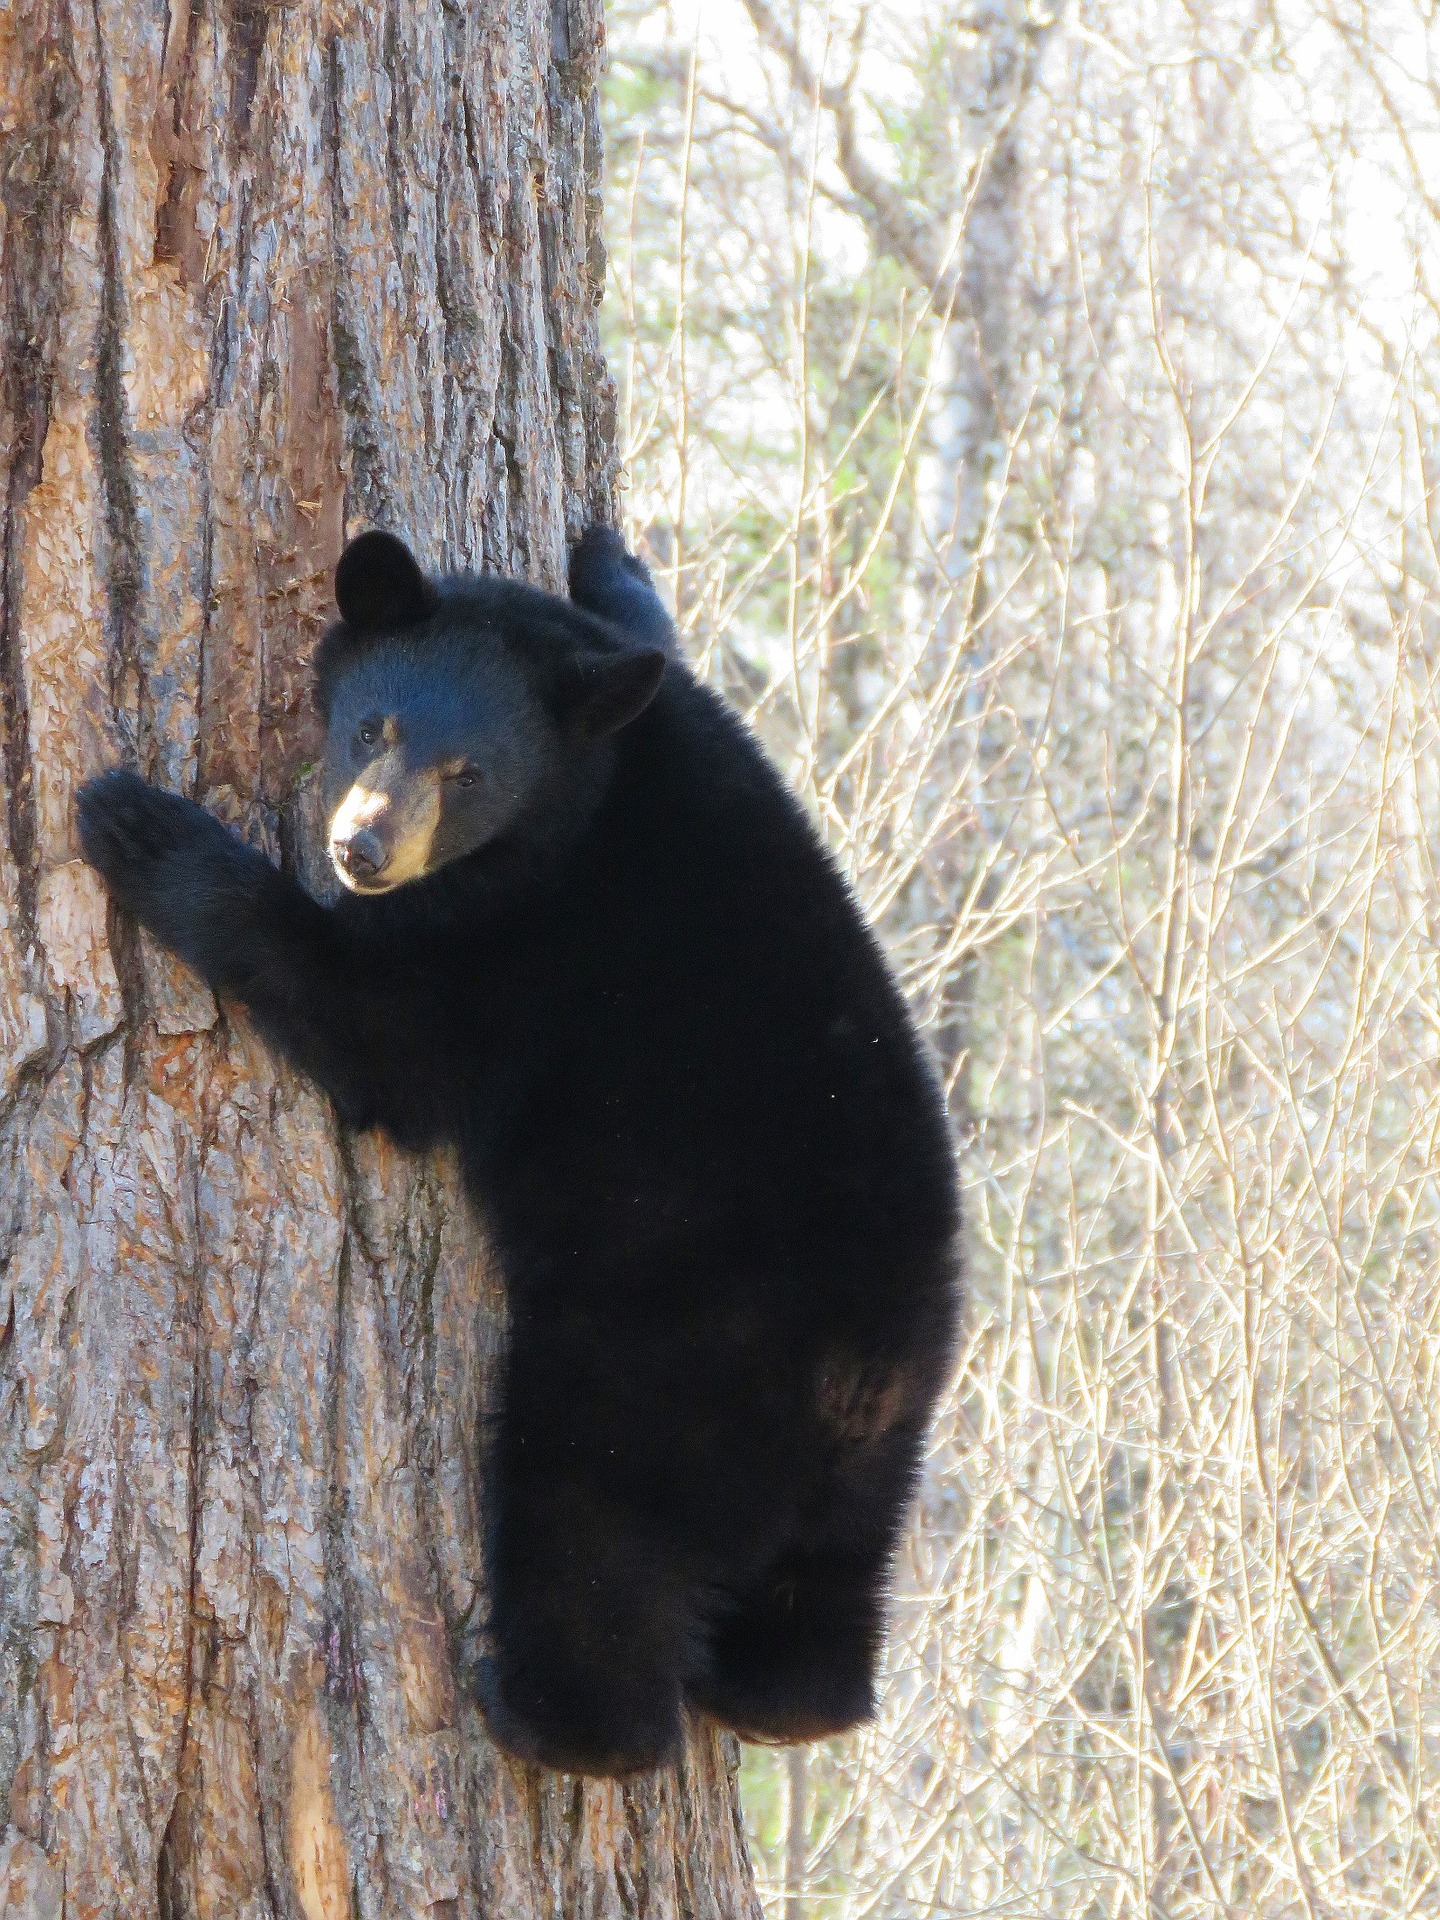
\includegraphics[trim={0 4cm 0 4cm},clip, width=0.65\textwidth]{images/bearcub.jpg}\\
		\hspace*{15pt}\hbox{\scriptsize Image By:\thinspace{\itshape Skeeze}}
		% https://pixabay.com/photos/bear-cub-brown-climbing-tree-1576559/
	\end{center}

\end{frame}

\begin{frame}
	\frametitle{Iterating over the nodes}
	
		\begin{block}{Finding all the nodes}
			If you want to iterate over the tree, you can do so in many different orders. Three common ones for binary trees are:
			\begin{itemize}
				\item Pre-order traversal
				\item In-order traversal
				\item Post-order traversal
			\end{itemize}
		\end{block}	
\end{frame}

\begin{frame}
	\frametitle{Pre-order traversal}
	\begin{overlayarea}{\textwidth}{\textheight}
			\begin{columns}
				\column{0.455\textwidth}
				\begin{itemize}
					\item First give the value of the current node.
					\item Then a pre-order traversal of the left child.
					\item Then a pre-order traversal of the right child.
				\end{itemize}
				\column{0.455\textwidth}
				\pause
					\begin{tikzpicture}[
						level distance = 2.5em,
						level 1/.style={sibling distance=9em},
						level 2/.style={sibling distance=4.5em},
						level 3/.style={sibling distance=2.25em},
					]
					\node[circle] (t1) {\alert<3>{1}}
					child { node[circle]   {\alert<4>{2}}
						child { node[circle] {\alert<5>{3}}}
						}
						child { node[circle]   {\alert<6>{4}}
							child { node[circle] {\alert<7>{5}}}
							child { node[circle] {\alert<8>{6}}
								child { node[circle] {\alert<9>{7}}}
								child { node[circle] {\alert<10>{8}}}
							}
						};
					\end{tikzpicture}
			\end{columns}
			\only<11>{
			\begin{block}{Amsterdam, Rotterdam, no not that kind of topology!}
				Gives us a \textit{topological} order of the tree.\\
				If all nodes represent jobs, and job $i$ depends on it's parent job $p$ then this gives us an order in which we can
				do all jobs, satisfying these dependencies.
			\end{block}
		}
	\end{overlayarea}
\end{frame}

\begin{frame}
	\frametitle{In-order traversal}
	\begin{overlayarea}{\textwidth}{\textheight}
			\begin{columns}
				\column{0.455\textwidth}
				\begin{itemize}
					\item First an in-order traversal of the left child.
					\item Then give the value of the current node.
					\item Then an in-order traversal of the right child.
				\end{itemize}
				\column{0.455\textwidth}
					\begin{tikzpicture}[
						level distance = 2.5em,
						level 1/.style={sibling distance=9em},
						level 2/.style={sibling distance=4.5em},
						level 3/.style={sibling distance=2.25em},
					]
					\node[circle] (t1) {\alert<5>{1}}
					child { node[circle]   {\alert<4>{2}}
						child { node[circle] {\alert<3>{3}}}
						}
						child { node[circle]   {\alert<7>{4}}
							child { node[circle] {\alert<6>{5}}}
							child { node[circle] {\alert<9>{6}}
								child { node[circle] {\alert<8>{7}}}
								child { node[circle] {\alert<10>{8}}}
							}
						};
					\end{tikzpicture}
			\end{columns}
			\only<2>{
				\begin{block}{In-order}
				What is the order of nodes now?
				% \begin{multicols}{2}
					\begin{enumerate}[A.]
						\item 1,2,3,4,5,6,7,8
						\item 3,2,1,5,4,7,6,8
						\item 3,2,8,7,6,5,4,1
						\item 8,7,6,5,4,3,2,1
					\end{enumerate}
				% \end{multicols}
			\end{block}
		}
			\only<11>{
				\begin{block}{We'll save that for tomorrow}
				We will see an example for this tomrrow!
			\end{block}
		}
	\end{overlayarea}
\end{frame}

\begin{frame}
	\frametitle{Post-order traversal}
	\begin{overlayarea}{\textwidth}{\textheight}
			\begin{columns}
				\column{0.455\textwidth}
				\begin{itemize}
					\item First a post-order traversal of the left child.
					\item Then a post-order traversal of the right child.
					\item Then give the value of the current node.
				\end{itemize}
				\column{0.455\textwidth}
					\begin{tikzpicture}[
						level distance = 2.5em,
						level 1/.style={sibling distance=9em},
						level 2/.style={sibling distance=4.5em},
						level 3/.style={sibling distance=2.25em},
					]
					\node[circle] (t1) {\alert<10>{1}}
					child { node[circle]   {\alert<4>{2}}
						child { node[circle] {\alert<3>{3}}}
						}
						child { node[circle]   {\alert<9>{4}}
							child { node[circle] {\alert<5>{5}}}
							child { node[circle] {\alert<8>{6}}
								child { node[circle] {\alert<6>{7}}}
								child { node[circle] {\alert<7>{8}}}
							}
						};
					\end{tikzpicture}
			\end{columns}
			\only<2>{
				\begin{block}{Post-order}
				What is the order of nodes now?
				% \begin{multicols}{2}
					\begin{enumerate}[A.]
						\item 1,2,3,4,5,6,7,8
						\item 3,2,5,8,7,6,4,1
						\item 3,2,8,7,6,5,4,1
						\item 8,7,6,5,4,3,2,1
					\end{enumerate}
				% \end{multicols}
			\end{block}
		}
			\only<11>{
				\begin{block}{I didn't mean to sound so dark :(}
				Used to delete a tree (first delete your children, before deleting yourself).
			\end{block}
		}
	\end{overlayarea}
\end{frame}

\begin{frame}
	\frametitle{It's all about balance}
	\begin{center}
		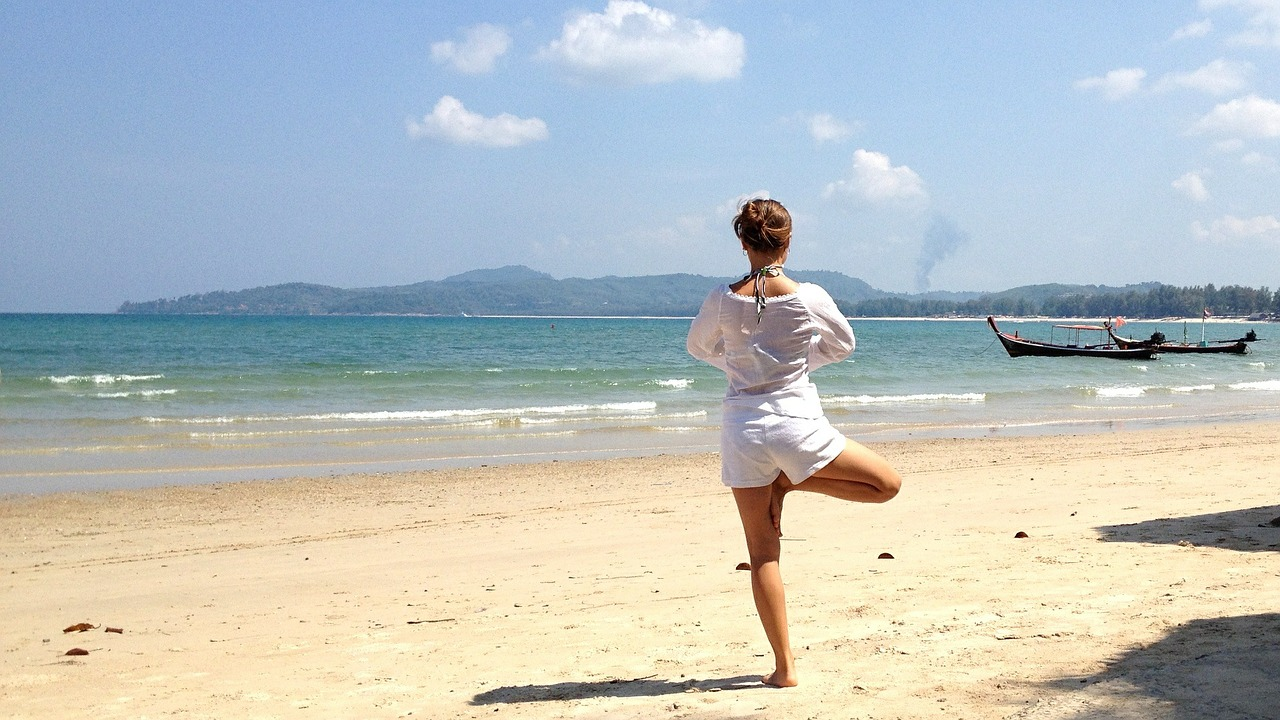
\includegraphics[width=0.8\textwidth]{images/balance.jpg}\\
		\hspace*{15pt}\hbox{\scriptsize Image By:\thinspace{\itshape Evitaochel}}
		% https://pixabay.com/photos/balance-yoga-zen-exercise-405513/
	\end{center}
\end{frame}

\begin{frame}
	\frametitle{Limiting the height}
	\begin{block}{The idea}
		If we can somehow limit the height to be $\Theta(\log n)$ we are all set.
	\end{block}	
	\pause
	This is where the tens of options come in...
	\begin{itemize}
		\item AVL-trees
		\item Red-Black trees
		\item Splay-trees
		\item And many more\dots
	\end{itemize}
\end{frame}

\begin{frame}
	\frametitle{AVL-Trees}
	\framesubtitle{Named after Adel'son-Vel'skii and Landis}

		\begin{block}{AVL-trees}
			It is a binary search tree, with one more constraint:\\
			The height of the left-subtree and right-subtree of a node differ by at most 1 for all nodes in the tree.
		\end{block}	

	\begin{columns}
		\column{0.455\textwidth}

		\begin{tikzpicture}[
			level distance = 2.5em,
			level 1/.style={sibling distance=9em},
			level 2/.style={sibling distance=4.5em},
			level 3/.style={sibling distance=2.25em},
			]
			\node[circle] (t1) {12}
			child { node[circle]   {3}
				child[draw=white] { }
				child { node[circle] {9}}
			}
			child { node[circle]   {25}
				child { node[circle] {14}}
				child { node[circle] {29}
					child { node[circle] {26}}
					child { node[circle] {32}}
				}
			};
		\end{tikzpicture}
		\column{0.455\textwidth}

		\begin{block}{Is it full?}
			Is this tree an AVL-tree?
		\end{block}
		\pause
		\begin{block}{}
			Yes :)	
		\end{block}
	\end{columns}
\end{frame}

\begin{frame}
	\frametitle{AVL-trees}
	\begin{block}{Height}
		This guarantees the height to be $\Theta(\log n)$ (check the book for a proof if you want).
	\end{block}

	\pause
	\begin{block}{Inserting/deleting nodes}
		How do we now insert or delete nodes from this AVL tree?
	\end{block}
\end{frame}

\begin{frame}
	\frametitle{Inserting items}

	\begin{block}{Observations}
		\begin{itemize}
			\item If we insert like we did in a ``regular'' binary search tree\dots
			\item Then we only upset (potentially) the ancestors of the node where we insert it.
				\pause
			\item Let's look at an example ;)
		\end{itemize}
	\end{block}	
	\pause
	\begin{block}{Inserting an item}
		\begin{columns}
			\column{0.455\textwidth}

			\begin{tikzpicture}[
				level distance = 2.5em,
				level 1/.style={sibling distance=9em},
				level 2/.style={sibling distance=4.5em},
				level 3/.style={sibling distance=2.25em},
				scale=0.8,transform shape
				]
				\node[circle] (t1) {12}
				child { node[circle]   {3}
					child[draw=white] { }
					child { node[circle] {9}}
				}
				child { node[circle]   {\alt<6>{\color{blue}26}{25}}
					child { node[circle] {\alt<6>{\color{blue}{25}}{14}}
						child[] { node[circle] {\alt<6>{\color{blue}{14}}{}}}
						child[draw=white] { }
					}
					child { node[circle] {29}
						child { node[circle] {\alt<6>{\color{blue}27}{26}}
							child[draw=white] { }
							child[] { node[circle] {\alt<6>{}{27}}}
						}
						child { node[circle] {32}}
					}
				};
			\end{tikzpicture}
			\column{0.455\textwidth}
			\begin{itemize}
				\item Two items are now upsetting the AVL-property.
					\pause
				\item So we need to fix that!
					\pause
				\item We can do so by \textit{rotating} some nodes around.
					\pause
				\item To end up with this.
			\end{itemize}
		\end{columns}
	\end{block}	
\end{frame}

\begin{frame}
	\frametitle{A tri-node restructering}
	\framesubtitle{Draw this for yourself!}
	\vspace{-15pt}
	\begin{columns}
		\column{0.455\textwidth}
			\begin{tikzpicture}[
				level distance = 2.5em,
				level 1/.style={sibling distance=9em},
				level 2/.style={sibling distance=5.5em},
				level 3/.style={sibling distance=4.5em},
				child anchor =north
				]
				\node[circle] (t1) {z}
				child { node[draw=black, anchor = north]   {T1}
				}
				child { node[circle]   {y}
					child { node[circle] {x}
						child { node[circle, anchor = north, draw=black] {T2}}
						child { node[circle, anchor = north, draw=black] {T3}}
					}
					child { node[circle, anchor = north, draw=black] {T4}
					}
				};
			\end{tikzpicture}
		\column{0.455\textwidth}
		\begin{itemize}
			\item This is the situation before inserting (we chose these heights to make the insertion interesting).
				\pause
				\begin{itemize}
					\item $z$ has a height of $h+2$
					\item $y$ has a height of $h+1$
					\item $x$ has a height of $h$
					\item $T1,T4$ have a height of $h$
					\item $T2,T3$ have a height of $h-1$
				\end{itemize}
				\pause
			\item We now insert an item into T3, which causes an imbalance in node z.
				\pause
				\begin{itemize}
					\item $z$ has a height of $h+3$
					\item $y$ has a height of $h+2$
					\item $x$ has a height of $h+1$
					\item $T1,T3,T4$ have a height of $h$
					\item $T2$ has a height of $h-1$
				\end{itemize}
		\end{itemize}
			
	\end{columns}
\end{frame}

\begin{frame}
	\frametitle{A tri-node restructering}
	\framesubtitle{Draw this for yourself!}
	\vspace{-15pt}
	\begin{columns}
		\column{0.455\textwidth}
			\begin{tikzpicture}[
				level distance = 2.5em,
				level 1/.style={sibling distance=9.5em},
				level 2/.style={sibling distance=5.0em},
				child anchor =north
				]
				\node[circle] (t1) {x}
				child { node[circle]   {z}
					child { node[draw=black, anchor = north]   {T1}
					}
					child { node[draw=black, anchor = north]   {T2}
					}
			}
				child { node[circle]   {y}
					child { node[circle, anchor = north, draw=black] {T3}}
					child { node[circle, anchor = north, draw=black] {T4}
					}
				};
			\end{tikzpicture}
		\column{0.455\textwidth}
		\begin{itemize}
			\item We can now rotate some stuff around :)
			\item Notice that the subtrees have not changed.
				\begin{itemize}
					\item $T1,T3,T4$ have a height of $h$
					\item $T2$ has a height of $h-1$
						\pause
					\item $z$ now has a height of $h+1$
					\item $y$ now has a height of $h+1$
					\item $x$ now has a height of $h+2$
				\end{itemize}
		\end{itemize}
			
	\end{columns}

	
\end{frame}

\begin{frame}
	\frametitle{Let's help ourselves}
	\begin{columns}
		\column{0.455\textwidth}
			
			\begin{tikzpicture}[
				level distance = 2.5em,
				level 1/.style={sibling distance=9em},
				level 2/.style={sibling distance=4.5em},
				level 3/.style={sibling distance=3em},
				level 4/.style={sibling distance=2em},
				]
				\node[circle] (t1) {12}
				child { node[circle]   {3}
					child { node[circle] {$\square$} }
					child { node[circle] {9}
						child { node[circle] {$\square$} }
						child { node[circle] {$\square$} }
					}
				}
				child { node[circle]   {25}
					child { node[circle] {14}
						child { node[circle] {$\square$} }
						child { node[circle] {$\square$} }
					}
					child { node[circle] {29}
						child { node[circle] {26}
							child { node[circle] {$\square$} }
							child { node[circle] {27}}
						}
						child { node[circle] {32}
							child { node[circle] {$\square$} }
							child { node[circle] {$\square$} }
						}
					}
				};
			\end{tikzpicture}
		\column{0.455\textwidth}
		\begin{itemize}
			\item Let's draw the non-existing leafs!
			\item This will help us identify what to rotate :)
				\pause
			\item And let's do this on the board.
		\end{itemize}
	\end{columns}
\end{frame}

\begin{frame}
	\frametitle{Phew...}
	\begin{center}
		
\includegraphics[width=0.5\textwidth]{images/relief.png}\\
		\hspace*{15pt}\hbox{\scriptsize Image By:\thinspace{\itshape Twitter}}
	\end{center}
	
\end{frame}

\begin{frame}
	\frametitle{Deletion}
	\framesubtitle{No! Not another}
		\begin{block}{Deleting a node}
			Also requires just one rotation to fix the imbalance.
		\end{block}	
		\pause
			\begin{block}{Tutorial time}
			  But we'll save that for the tutorial tomorrow.	
			\end{block}	
\end{frame}


\begin{frame}
	\frametitle{Binary Search Trees}
	\begin{center}
		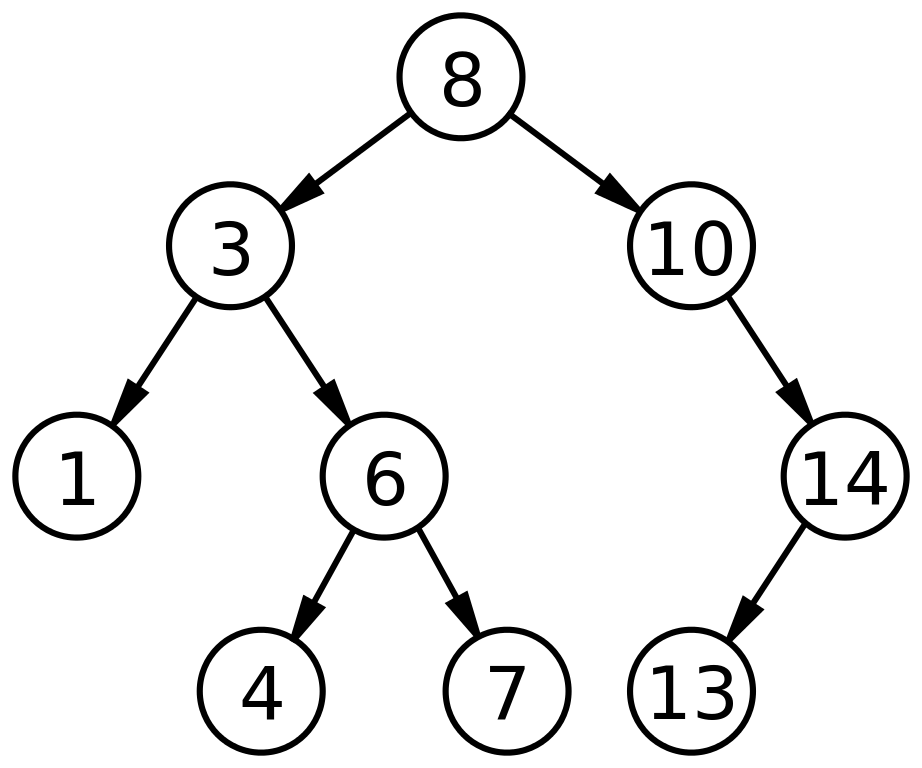
\includegraphics[width=0.5\textwidth]{images/btree.png}\\
		\hspace*{15pt}\hbox{\scriptsize Image By:\thinspace{\itshape Derrick Coetzee}}
		% https://en.wikipedia.org/wiki/File:Binary_search_tree.svg
	\end{center}
\end{frame}

\begin{frame}
	\frametitle{Binary Search Trees}
	
	\begin{block}{Binary \alert{Search} Trees}
		\begin{itemize}
			\item Every node has at most 2 children.
				\pause
			\item The left descendants have a smaller value than the node.
			\item The right descendants have a larger value than the node.
		\end{itemize}
	\end{block}	
	\pause
	\begin{columns}
		\column{0.455\textwidth}

		\begin{tikzpicture}[
			level distance = 2.5em,
			level 1/.style={sibling distance=9em},
			level 2/.style={sibling distance=4.5em},
			level 3/.style={sibling distance=2.25em},
			]
			\node[circle] (t1) {12}
			child { node[circle]   {3}
				child { node[circle] {2}}
				child { node[circle] {9}}
			}
			child { node[circle]   {25}
				child { node[circle] {14}}
				child { node[circle] {29}
					child { node[circle] {26}}
					child { node[circle] {32}}
				}
			};
		\end{tikzpicture}
		\column{0.455\textwidth}

		\begin{block}{Is it full?}
			Is this tree a binary search tree?
		\end{block}
		\pause
		\begin{block}{}
			Yes :)	
		\end{block}
	\end{columns}
\end{frame}

\begin{frame}
	\frametitle{Searching in a Binary SearchTree}
	
	\vspace{-20pt}
	\begin{overlayarea}{\textwidth}{\textheight}
		\begin{block}{Searching}
			So, how quickly can we search for an item in a Binary Search Tree?
			\only<1>{
			\begin{enumerate}[A.]
				\item $\Theta(\log h)$
				\item $\Theta(h)$
				\item $\Theta(\log n)$
				\item $\Theta(n)$
				\item $\Theta($\textit{I don't know man}$)$
			\end{enumerate}
		}
		\end{block}
		\pause
		\lstinputlisting{src/search_btree.py}
		\pause
	\vspace{-10pt}
		\begin{block}{Only one path}
			So $\Theta(h)$
		\end{block}
	\end{overlayarea}
\end{frame}

\begin{frame}
	\frametitle{MinMaxing}
	
	\begin{overlayarea}{\textwidth}{\textheight}
		\begin{block}{Minmaxing like a real gamer}
			So, how quickly can we find the minimum or maximum in a Binary Search Tree?
			\only<1>{
			\begin{enumerate}[A.]
				\item $\Theta(\log h)$
				\item $\Theta(h)$
				\item $\Theta(\log n)$
				\item $\Theta(n)$
				\item $\Theta($\textit{Something?}$)$
			\end{enumerate}
		}
		\end{block}
		\pause
		\lstinputlisting{src/minmax_btree.py}
		\pause
		\begin{block}{Only one path}
			So $\Theta(h)$
		\end{block}
	\end{overlayarea}
\end{frame}

\begin{frame}
	\frametitle{Inserting or Deleting an item}

	\begin{block}{Inserting an item}
		Find the right place in $\Theta(h)$ time, then put it there.
	\end{block}	

	\pause
	\begin{block}{Deleting an item}
		Find the item in $\Theta(h)$ time, then move either the left or right child up one level (and continue this down the
		path to a leaf).
	\end{block}	
	\pause
		\begin{block}{Sorting the list}
			Oh and by the way, this is where the in-order traversal can get us a sorted list of all items in the tree!
		\end{block}	
\end{frame}


\begin{frame}
	\frametitle{So in summary}
	\begin{tabular}{r | l}
		Operation & Time \\
		\midrule
		Insert & $\Theta(h)$ \\
		Delete & $\Theta(h)$ \\
		Search & $\Theta(h)$ \\
		Min & $\Theta(h)$ \\
		Max & $\Theta(h)$ \\
	\end{tabular}
	\pause	
	\begin{block}{So how bad is it?}
		What is the worst-case $h$, and how do we get that?
	\end{block}
	\pause
	\begin{block}{Inserting a sorted list}
		Insert a sorted list, and what happens? \\
		\pause 
		We get a tree with only right children (or only left if the list is sorted descendingly).
	\end{block}
	
\end{frame}


\begin{frame}
	\frametitle{Generalising a bit}
		\begin{block}{Multiway search tree}
			\begin{itemize}
				\item Each node of $T$ has \textit{at least} 2 children (except for leaves of course).
				\item Each $d$-node (where $d$ is the amount of children the node has), stores $d-1$ values in increasing value.
				\item Between two keys $i$ and $i+1$ stored in the node, is rooted a tree that contains only keys $k$ such that
					$k_i \leq k \leq k_{i+1}$.
			\end{itemize}
			
		\end{block}	

		\begin{tikzpicture}[
			level distance = 2.5em,
			level 1/.style={sibling distance=14em},
			level 2/.style={sibling distance=4.5em},
			level 3/.style={sibling distance=2.25em},
			level 3/.style={sibling distance=4em},
			]
			\node[circle, draw] (t1) {22}
			child { node[circle, draw]   {5\quad10}
				child { node[circle, draw] {3\quad4}}
				child { node[circle, draw] {6\quad8}}
				child { node[circle, draw] {14}
					child { node[circle, draw] {11\quad13}}
					child { node[circle, draw] {17}}
				}
			}
			child { node[circle, draw]   {25}
				child { node[circle, draw] {23\quad24}}
				child { node[circle, draw] {27}}
			};
		\end{tikzpicture}
	
\end{frame}

\begin{frame}
	\frametitle{Practice?}
	
		\begin{block}{What should you know?}
			\begin{itemize}
				\item You should be able to search for items in a multiway search tree.
				\item And in the lab you will practice a bit with inserting nodes. Read the book carefully, it's not trivial!
				\item On the computer exam, we will not ask you to implement insertion or deletion in multiway search trees.
			\end{itemize}
		\end{block}	
\end{frame}


\begin{frame}
	\frametitle{Recap}
	
		\begin{block}{Binary Trees}
			\begin{itemize}
				\item Every node has at most 2 children.
					\pause
				\item One \textit{left} child and one \textit{right} child.
			\end{itemize}
		\pause
		A binary tree is \textit{proper} or \textit{full} if all nodes have either 0 or 2 children.
		\end{block}	
		\pause
		\begin{columns}
			\column{0.455\textwidth}
				
			\begin{tikzpicture}[
				level distance = 2.5em,
				level 1/.style={sibling distance=9em},
				level 2/.style={sibling distance=4.5em},
				level 3/.style={sibling distance=2.25em},
			]
			\node[circle] (t1) {root}
				child { node[circle]   {child 1}
					child { node[circle] {l1}}
					child { node[circle] {l2}}
				}
				child { node[circle]   {child 2}
					child { node[circle] {\alert<3>{l3}}}
					child { node[circle] {\alert<3>{l4}}
						child { node[circle] {\alert<3>{l5}}}
						child { node[circle] {\alert<3>{l6}}}
					}
				};
			\end{tikzpicture}
			\column{0.455\textwidth}
				
			\begin{block}{Is it full?}
				Is this tree full?
			\end{block}
			\begin{block}{}
				Yes :)	
			\end{block}
		\end{columns}
\end{frame}

\begin{frame}
	\frametitle{Recap of Trees}
	\begin{columns}
		\column{0.405\textwidth}
			\begin{tikzpicture}[
				level distance = 2.5em,
				level 1/.style={sibling distance=9em},
				level 2/.style={sibling distance=4.5em},
				level 3/.style={sibling distance=2.25em},
			]
			\node[circle] (t1) {root}
				child { node[circle] {child 1}
					child { node[circle] {leaf 1}}
				}
				child { node[circle] {child 2}
					child { node[circle] {leaf 2}}
					child { node[circle] {leaf 3}}
					child { node[circle] {leaf 4}}
				};
			\end{tikzpicture}
		\column{0.555\textwidth}
		\begin{itemize}
			\item The \textit{root node} is the node that has no \textit{parent}.
			\item A node can have \textit{children}.
			\item A node without children is called a \textit{leaf}.
			\item Two nodes with the same \textit{parent} are \textit{siblings}.
			\item \textit{Descendants} are found by repeatedly following child-relations.
			\item \textit{Ancestors} are found by repeatedly following parent-relations.
		\end{itemize}
	\end{columns}
\end{frame}

%%%%%%%%%%%%%%%%%%%%%%%%%%%%%%%%%%%%%%%%%%%%%%%%%%%%%%%%%%%%%%%%%%%%%%
\begin{frame}[fragile]\frametitle{}
\begin{center}
{\Large Heaps}
\end{center}

\end{frame}


\begin{frame}
	\frametitle{Heaps}
	\framesubtitle{XKCD Tree: \url{https://xkcd.com/835}}
	\begin{center}
		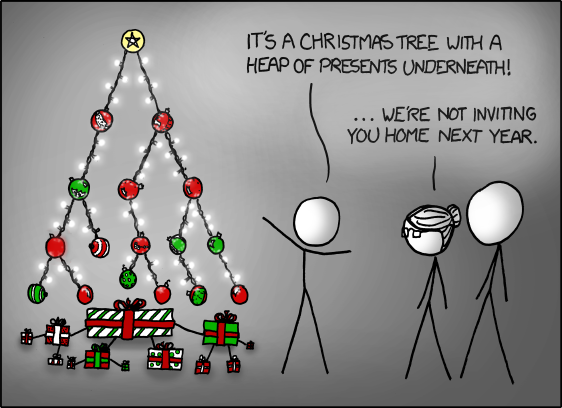
\includegraphics[width=0.6\textwidth]{images/tree.png}\\
	\end{center}
\end{frame}

\begin{frame}
	\frametitle{Heaps}
		\begin{block}{Heaps}
			We impose extra constraints and create a \textit{heap}:
			\begin{itemize}
				\item \textbf{Heap-order property:} For all nodes: The item stored in a node is greater than the item stored in its parent.
				\item \textbf{Complete Binary Tree property:} The tree is \textit{complete}: Meaning all layers are full, except possibly the last one which has only
					nodes in the left-most positions. 
			\end{itemize}
			\pause
			In this way, it is called a \textit{min-heap}. A \textit{max-heap} has the largest key in the root.
		\end{block}	
		\pause
		\begin{columns}
			\column{0.455\textwidth}

			\begin{tikzpicture}[
				level distance = 2.5em,
				level 1/.style={sibling distance=9em},
				level 2/.style={sibling distance=4.5em},
				level 3/.style={sibling distance=2.25em},
				]
				\node[circle] (t1) {1}
				child { node[circle]   {12}
					child { node[circle] {14}}
				}
				child { node[circle]   {4}
					child { node[circle] {5}}
					child { node[circle] {17}}
				};
			\end{tikzpicture}
			\column{0.455\textwidth}

			\begin{block}{Is it full?}
				Is this a correct min-heap?
			\end{block}
			\pause
			\vspace{-10pt}
			\begin{block}{Nope}
				No, as we do not use the left-most spots in the bottom layer.
			\end{block}
		\end{columns}
\end{frame}

\begin{frame}
	\frametitle{A use case}
	\framesubtitle{Me and my books, part 3}
	\begin{columns}
		\column{0.455\textwidth}
	\begin{center}
				\alt<5->{
					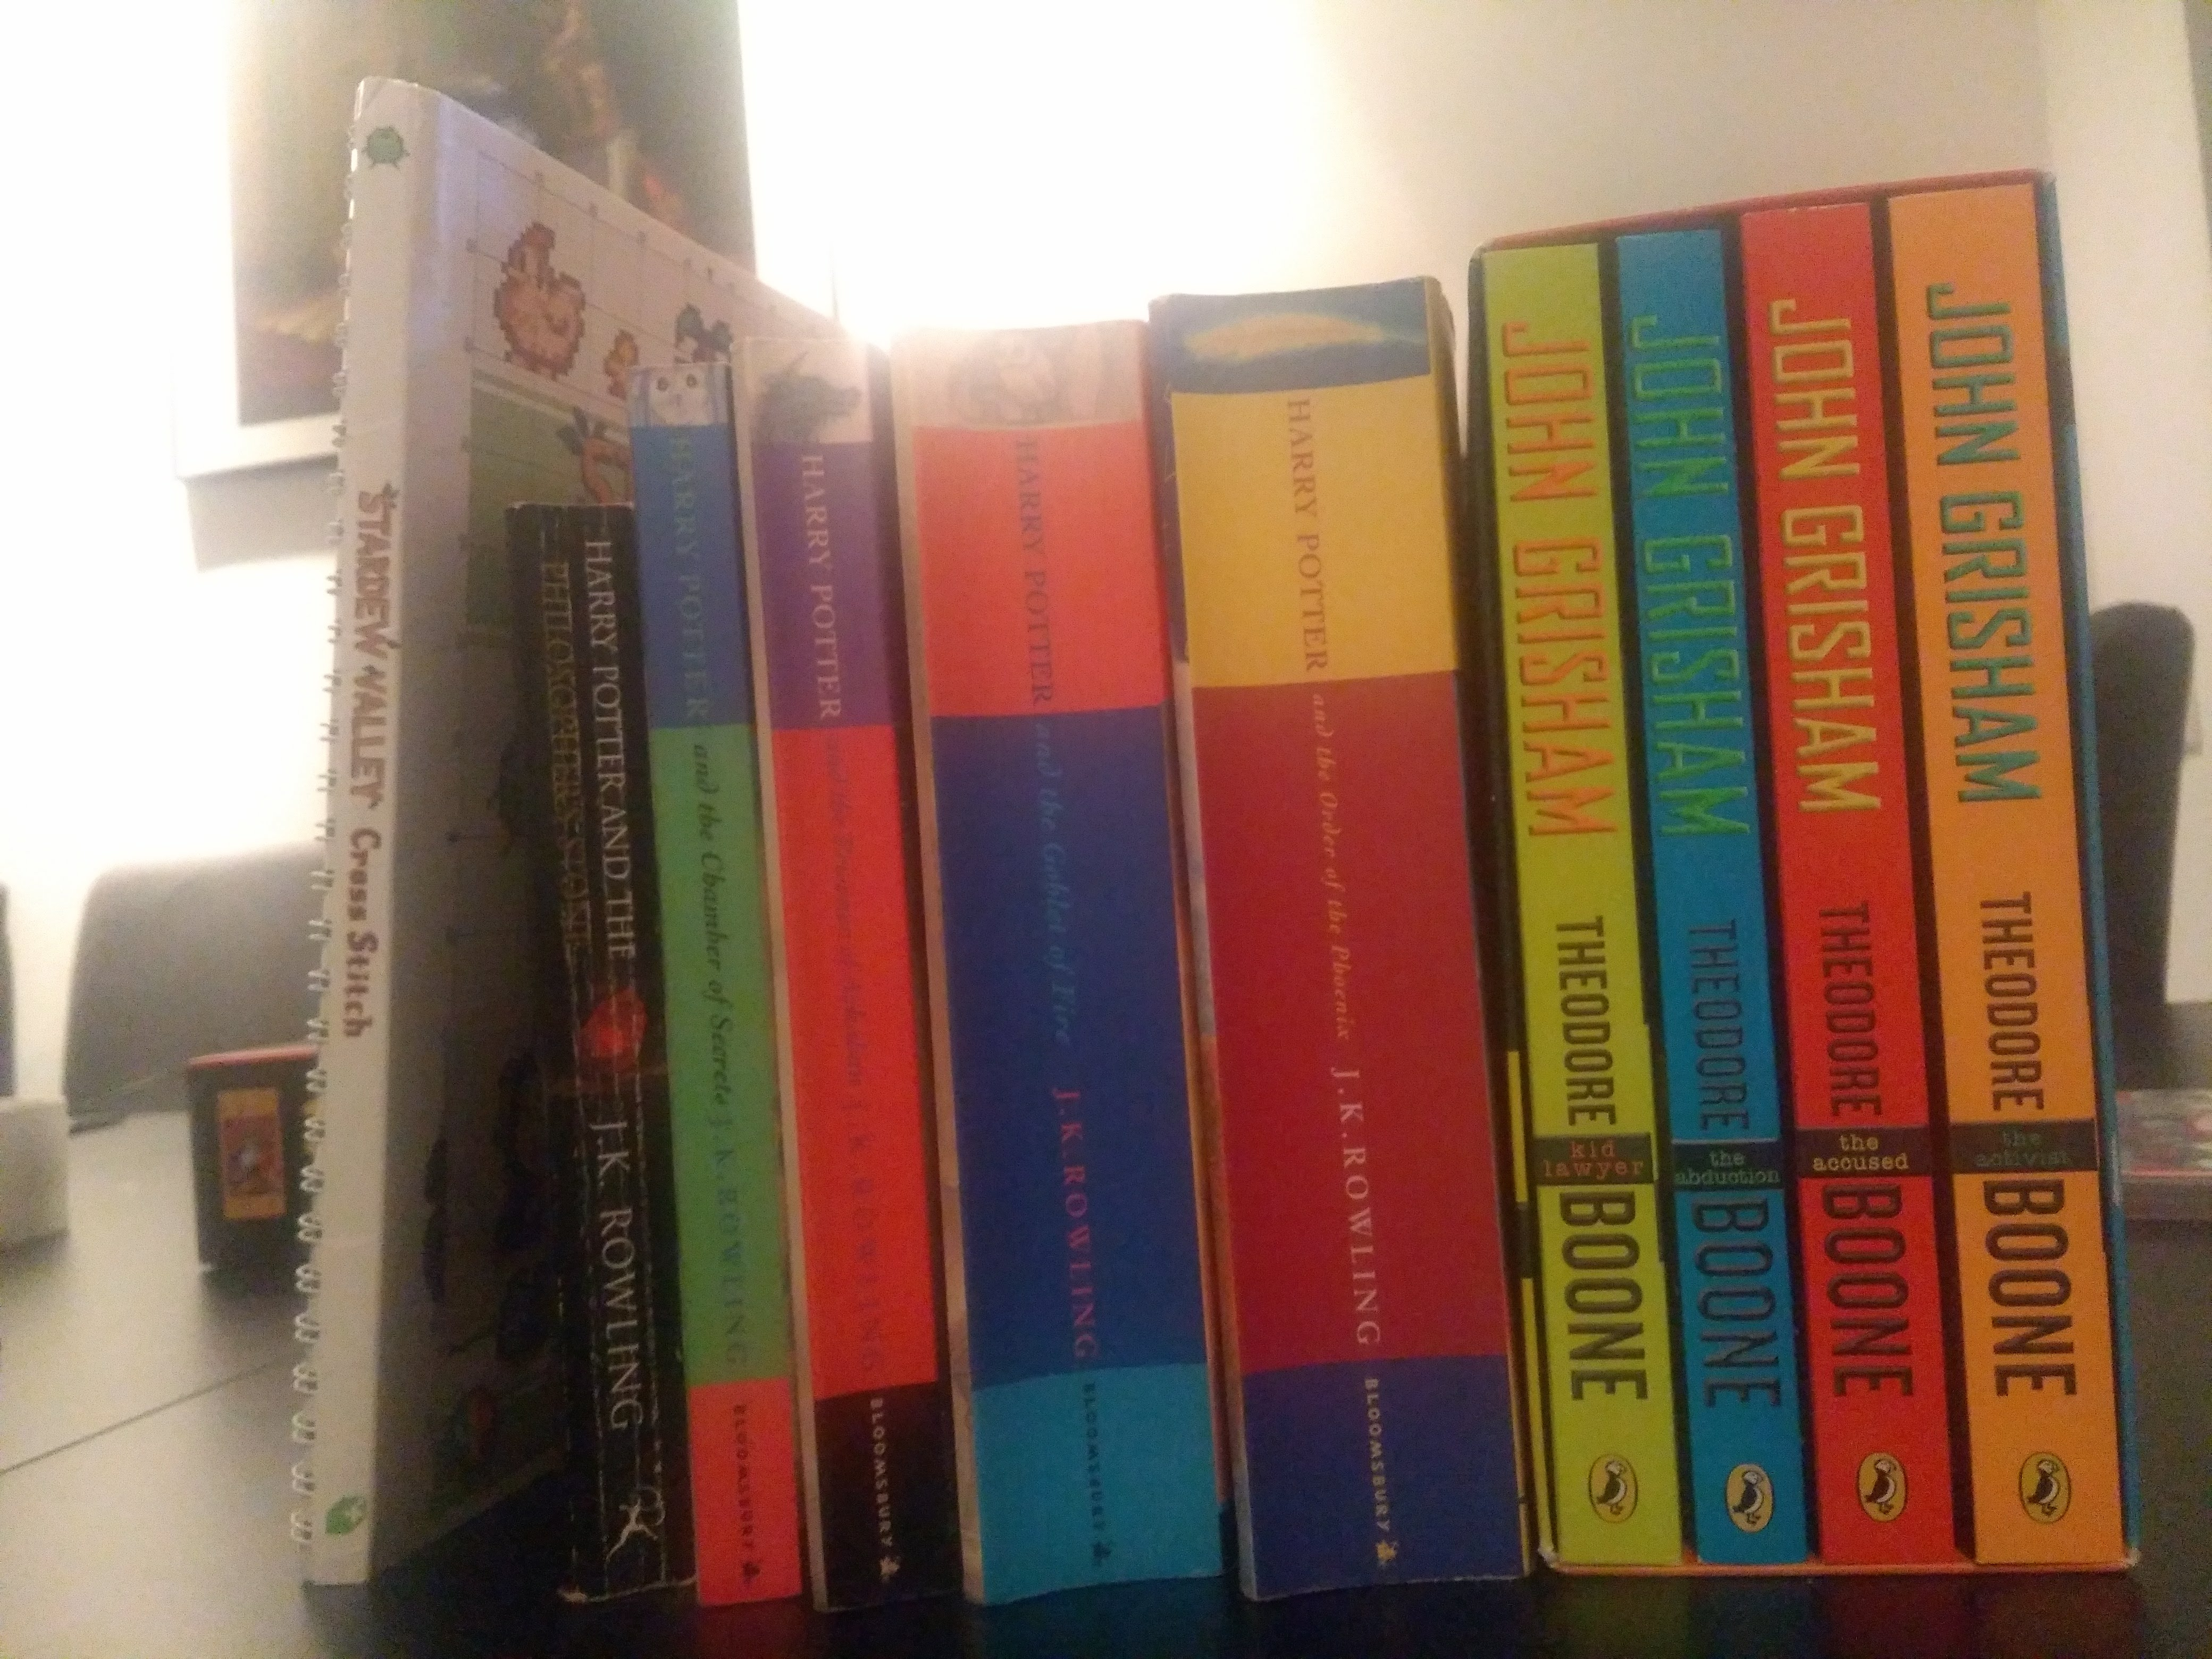
\includegraphics[width=\textwidth]{images/books_read.jpg}\\
					}{
					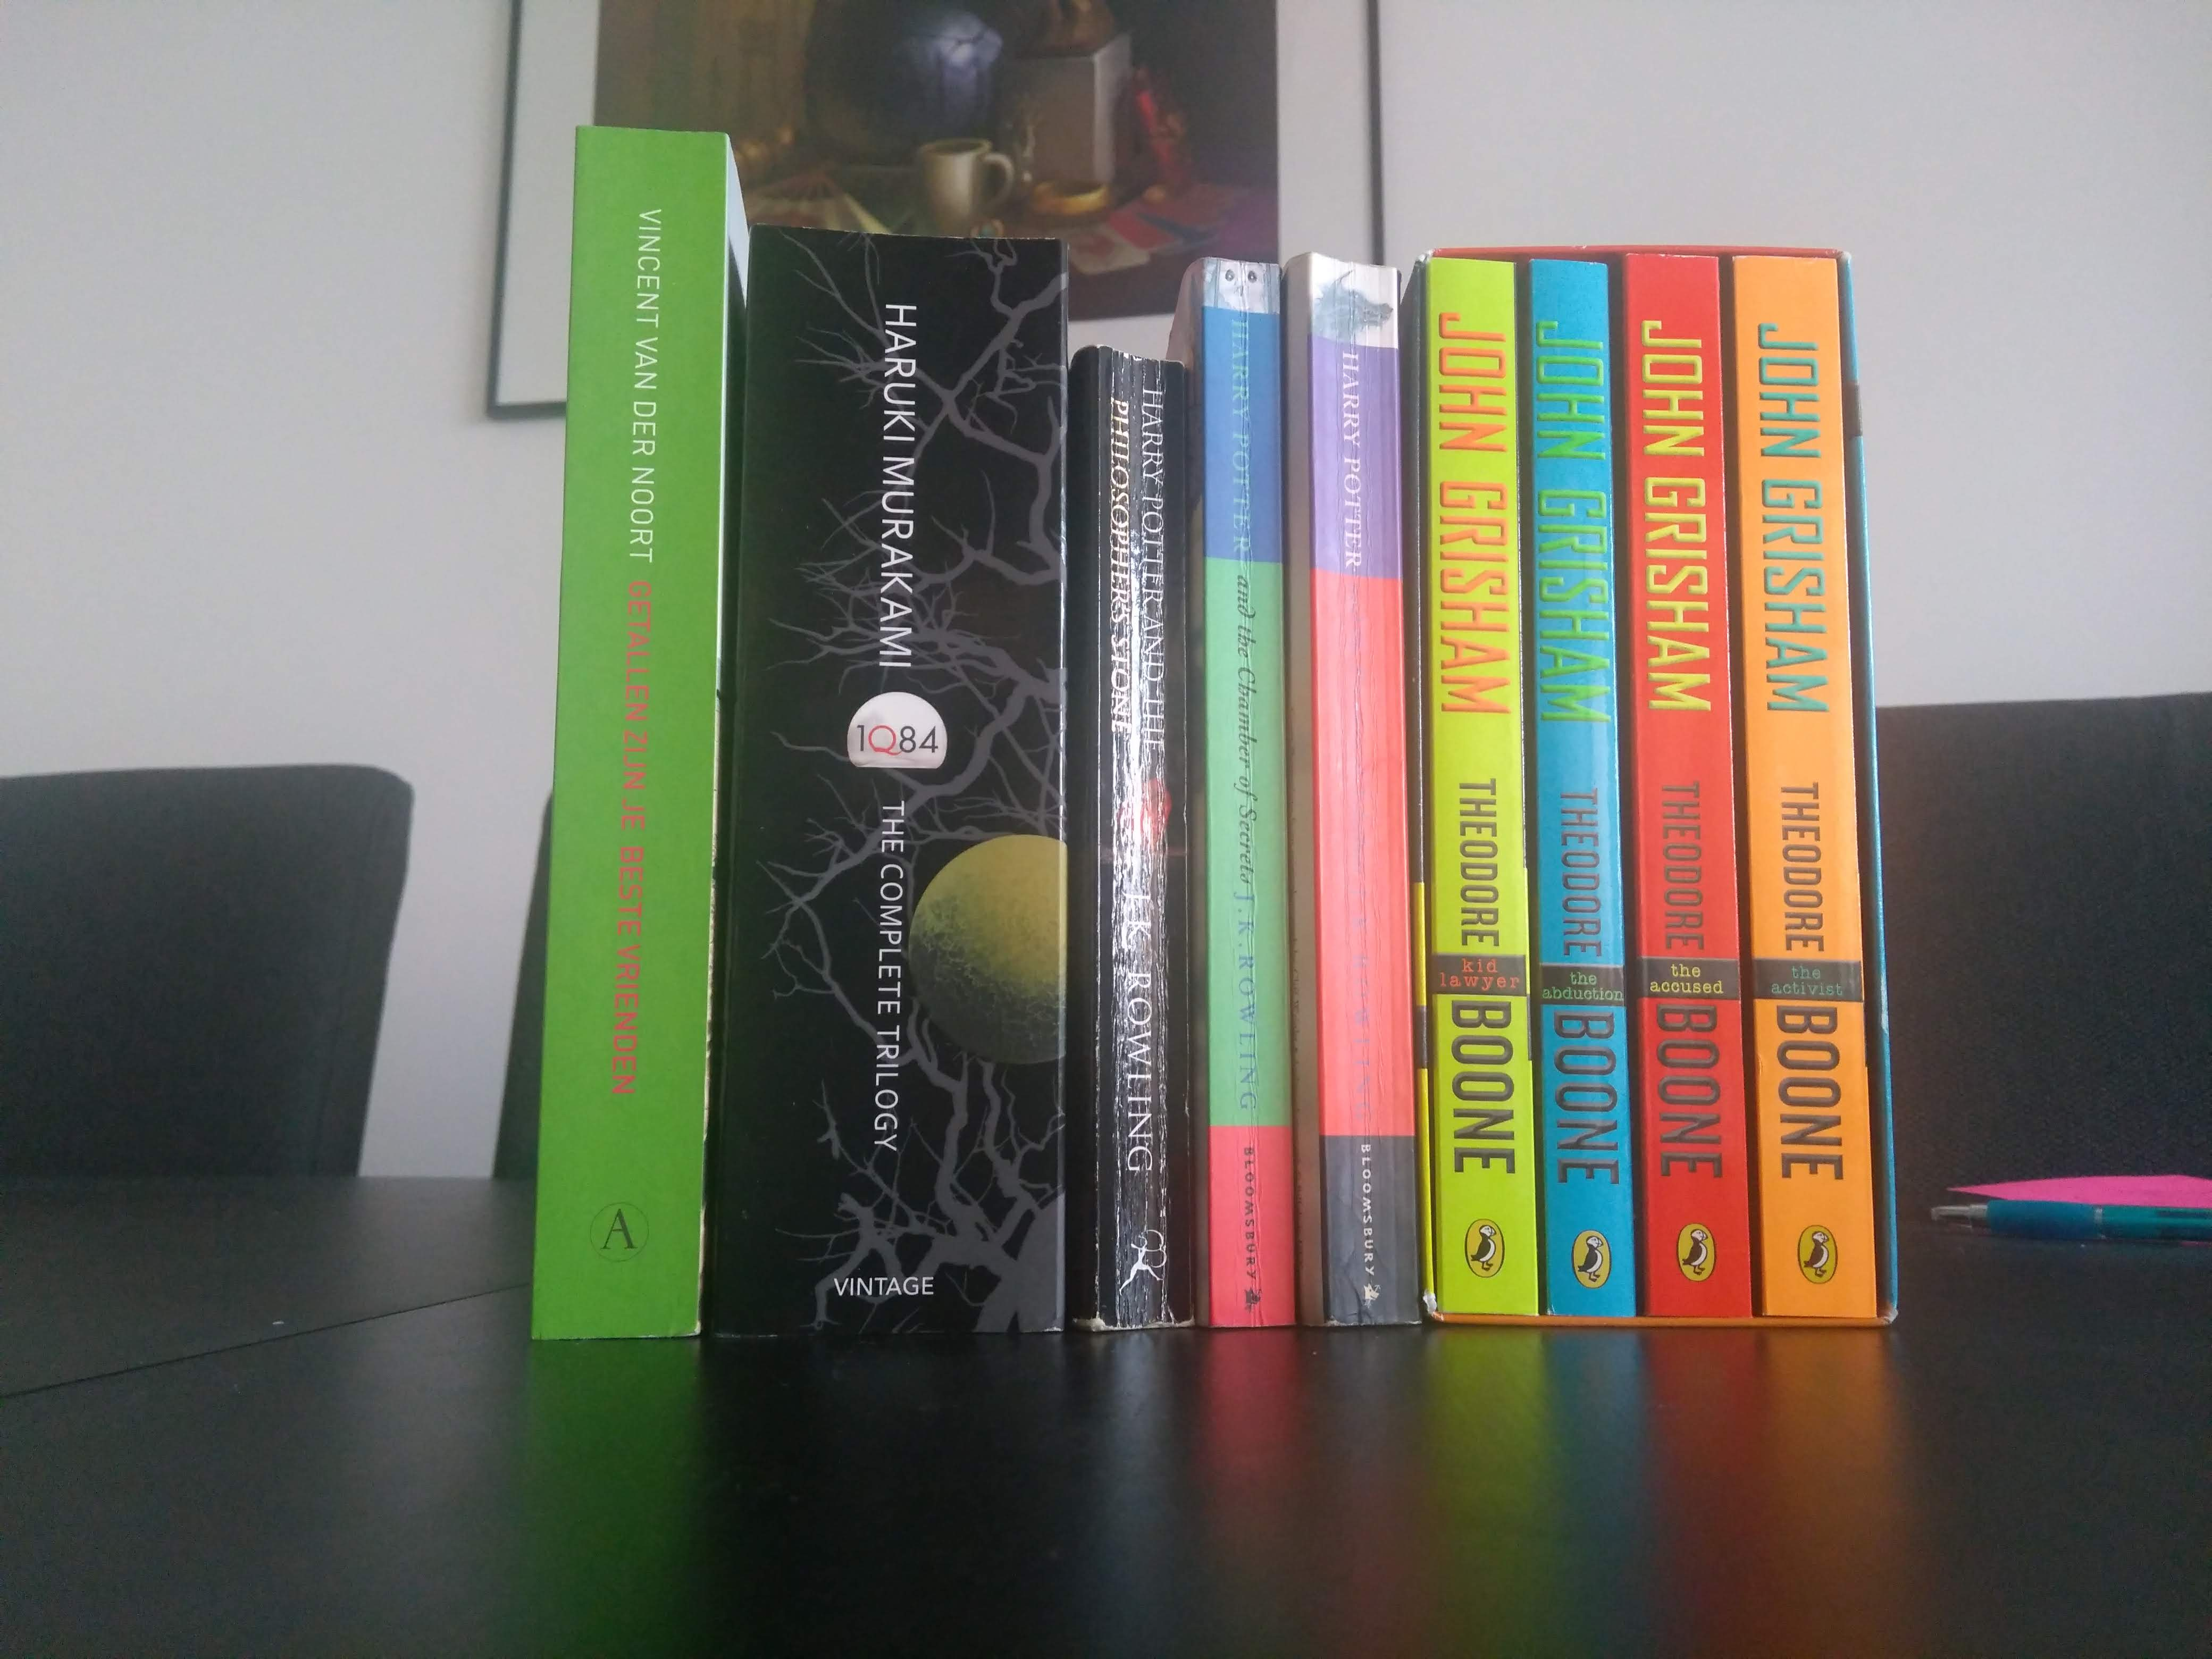
\includegraphics[width=\textwidth]{images/books_unread.jpg}\\
					}
		\hspace*{15pt}\hbox{\scriptsize Image By:\thinspace{\itshape Stefan Hugtenburg}}
		\hspace*{15pt}\hbox{\scriptsize Bookcovers and picture in the back by others}
	\end{center}
		\column{0.455\textwidth}
		\begin{itemize}
			\item There is more room for improvement.
				\pause
			\item A nice \alert{queue} of books.
				\pause
			\item After finishing one, I would take the next one from the left.
				\pause
			\item But what if a book should get \textit{priority}?
				\pause
			\item This uses a \textit{Priority Queue}, which we discuss in detail today.
		\end{itemize}
	\end{columns}
\end{frame}




\begin{frame}
	\frametitle{Bubbles!}
	\begin{center}
		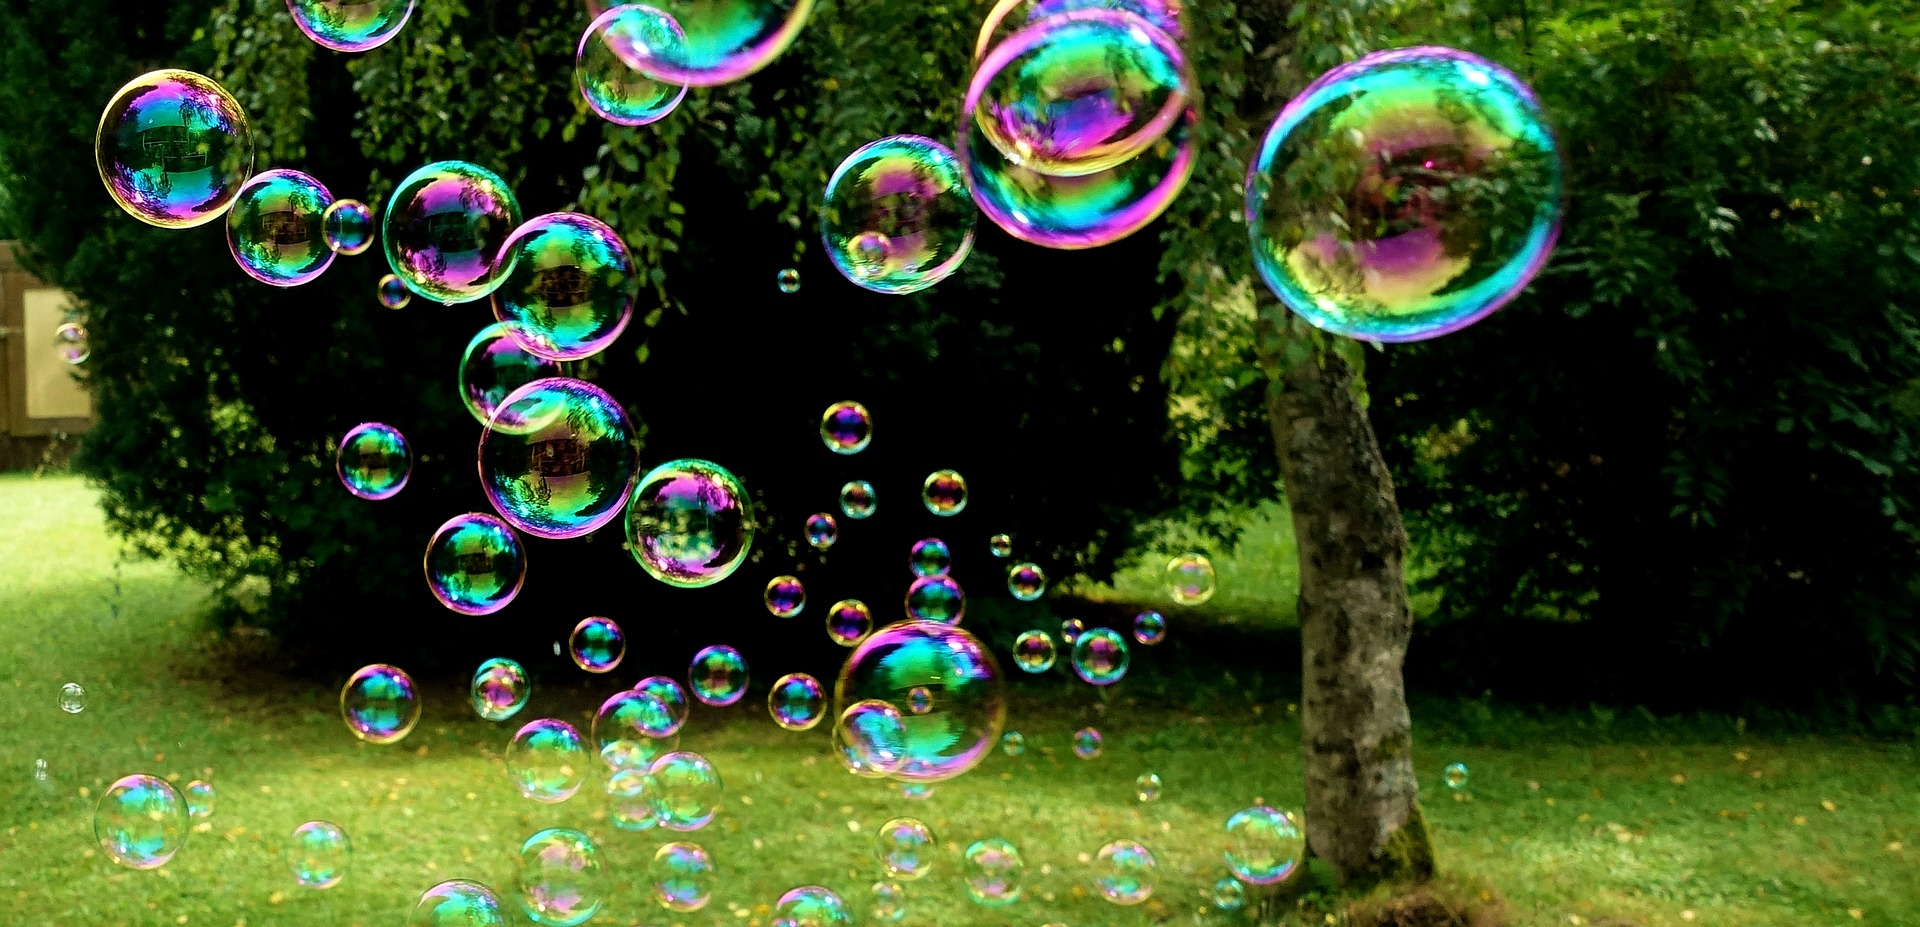
\includegraphics[width=0.8\textwidth]{images/bubble.jpg}\\
		\hspace*{15pt}\hbox{\scriptsize Image By:\thinspace{\itshape Alexas Fotos}}
		% https://pixabay.com/photos/soap-bubbles-colorful-flying-3517247/
	\end{center}
\end{frame}

\begin{frame}
	\frametitle{\alt<2->{A PriorityQueue ADT}{A Heap ADT}}
		\begin{block}{Heap, Heap, Array}
			There is no heap ADT per sé, it's just a special type of tree.
		\end{block}	
		\pause
		\begin{block}{PriorityQueue}
			But there is one for a PriorityQueue (which we could implement using a heap):
			\begin{itemize}
				\item \texttt{size()} (or \texttt{len} in Python) to get the number of elements.
					\pause
				\item \texttt{add(item)} to insert an item into the queue.
					\pause
				\item \texttt{remove\_min()} to remove the smallest element from the queue.
					\pause
				\item \texttt{min()} to get the smallest element from the queue.
			\end{itemize}
		\end{block}	
\end{frame}

\begin{frame}
	\frametitle{An array-based Priority Queue}

	\vspace{-20pt}
	\begin{columns}[t]
		\column{0.455\textwidth}
		\lstinputlisting{src/pq_array.py}
		\column{0.455\textwidth}
		\pause
		\begin{block}{Array-based PQ}
			We can easily create a PQ based on an array (or list).
		\end{block}	
		\pause
			\begin{block}{No, bad line graph!}
				But this makes \texttt{min} and \texttt{remove\_min} linear time operations!
			\end{block}	
			\pause
			\begin{block}{Can we do better?}
				Can we do better by using a sorted array?
			\end{block}
	\end{columns}
\end{frame}

\begin{frame}
	\frametitle{An sorted array-based Priority Queue}

	\vspace{-20pt}
	\begin{columns}[t]
		\column{0.455\textwidth}
		\lstinputlisting{src/pq_sortedarray.py}
		\column{0.455\textwidth}
		\pause
		\begin{block}{Array-based PQ}
			We can easily create a PQ based on a sorted array (or list).
		\end{block}	
		\pause
			\begin{block}{No, bad line graph!}
				But this makes \texttt{remove\_min} and \texttt{add} linear time operations!
			\end{block}	
			\pause
			\begin{block}{Can we do better?}
				Can we do better by using a heap?
			\end{block}
	\end{columns}
\end{frame}

\begin{frame}
	\frametitle{Min in a heap}
	\begin{block}{Consider a heap}
		How do I implement \texttt{min} for my heap-based PQ?
		\begin{enumerate}[A.]
			\item Return the value in the root.
			\item Return the value of the left-most descendant.
			\item Return the value of the right-most descendant.
			\item Go over all elements and return the minimum.
		\end{enumerate}
	\end{block}
	
	
\end{frame}

\begin{frame}
	\frametitle{Adding in a heap}
	\begin{block}{Consider a heap}
		Consider the following heap:\\
		\begin{columns}
			\column{0.455\textwidth}
			\begin{tikzpicture}[
				level distance = 2.5em,
				level 1/.style={sibling distance=9em},
				level 2/.style={sibling distance=4.5em},
				level 3/.style={sibling distance=2.25em},
				]
				\node[circle] (t1) {1}
				child { node[circle]   {12}
					child { node[circle] {14}}
					child { node[circle] {17}}
				}
				child { node[circle]   {4}
					child { node[circle] {5}}
				};
			\end{tikzpicture}
			\column{0.455\textwidth}
			\pause
			If I insert the element $7$ here, what should I do?
		\end{columns}
	\end{block}
	\begin{block}{Just add it at the bottom-right!}
			\begin{tikzpicture}[
				level distance = 2.5em,
				level 1/.style={sibling distance=9em},
				level 2/.style={sibling distance=4.5em},
				level 3/.style={sibling distance=2.25em},
				scale=0.8, transform shape
				]
				\node[circle] (t1) {1}
				child { node[circle]   {12}
					child { node[circle] {14}}
					child { node[circle] {17}}
				}
				child { node[circle]   {4}
					child { node[circle] {5}}
					child { node[circle] {7}}
				};
			\end{tikzpicture}
	\end{block}
\end{frame}

\begin{frame}
	\frametitle{Adding in a heap}
	\begin{block}{Consider a heap}
		Consider the following heap:\\
		\begin{columns}
			\column{0.455\textwidth}
			\begin{tikzpicture}[
				level distance = 2.5em,
				level 1/.style={sibling distance=9em},
				level 2/.style={sibling distance=4.5em},
				level 3/.style={sibling distance=2.25em},
				]
				\node[circle] (t1) {1}
				child { node[circle]   {12}
					child { node[circle] {14}}
					child { node[circle] {17}}
				}
				child { node[circle]   {4}
					child { node[circle] {5}}
				};
			\end{tikzpicture}
			\column{0.455\textwidth}
			\pause
			If I insert the element $0$ here, what should I do?
		\end{columns}
	\end{block}
	\begin{block}{Just add it at the bottom-right!}
		\begin{columns}
			\column{0.455\textwidth}
			\begin{tikzpicture}[
				level distance = 2.5em,
				level 1/.style={sibling distance=9em},
				level 2/.style={sibling distance=4.5em},
				level 3/.style={sibling distance=2.25em},
				scale=0.8, transform shape
				]
				\node[circle] (t1) {1}
				child { node[circle]   {12}
					child { node[circle] {14}}
					child { node[circle] {17}}
				}
				child { node[circle]   {4}
					child { node[circle] {5}}
					child { node[circle] {0}}
				};
			\end{tikzpicture}
			\column{0.455\textwidth}
			\pause
			And now fix the damage we have caused :)
		\end{columns}
	\end{block}
\end{frame}

\begin{frame}
	\frametitle{Up-bubbling}

	\begin{block}{Fixing the damage}
		How can we fix the damage caused to the heap \textit{efficiently}?
		\begin{columns}
			\column{0.455\textwidth}
			\begin{tikzpicture}[
				level distance = 2.5em,
				level 1/.style={sibling distance=9em},
				level 2/.style={sibling distance=4.5em},
				level 3/.style={sibling distance=2.25em},
				scale=0.8, transform shape
				]
				\node[circle] (t1) {1}
				child { node[circle]   {12}
					child { node[circle] {14}}
					child { node[circle] {17}}
				}
				child { node[circle]   {4}
					child { node[circle] {5}}
					child { node[circle] {0}}
				};
			\end{tikzpicture}
			\column{0.455\textwidth}
			\pause
			\begin{enumerate}[A.]
				\item Swap it with the root element and then swap it down as needed.
				\item Repeatedly compare the new node with the siblings and swap if needed.
				\item Repeatedly compare the new node with the parent and swap if needed.
				\item We cannot, we have to rebuild the entire heap.
			\end{enumerate}
		\end{columns}
	\end{block}
\end{frame}

\begin{frame}
	\frametitle{Up-bubbling}

	\begin{block}{Fixing the damage}
		Repeatedly switch with the parent if needed.\\
		\begin{columns}
			\column{0.455\textwidth}
				
			\begin{tikzpicture}[
				level distance = 2.5em,
				level 1/.style={sibling distance=9em},
				level 2/.style={sibling distance=4.5em},
				level 3/.style={sibling distance=2.25em},
				scale=0.8, transform shape
				]
				\node[circle] (t1) {\alt<5->{\alert<5>{0}}{1}}
				child { node[circle]   {12}
					child { node[circle] {14}}
					child { node[circle] {17}}
				}
				child { node[circle] {\alt<5->{\alert<5>{1}}{\alt<3->{\alert<3>{0}}{4}}}
					child { node[circle] {5}}
					child { node[circle] {\alt<3->{\alert<3>{4}}{0}}}
				};
			\end{tikzpicture}
			\column{0.455\textwidth}
			\only<6->{
			\begin{itemize}
				\item Notice how the left half of the tree has not been touched at all!
				\item Only one path changes!
			\end{itemize}	
	}
		\end{columns}
	\end{block}
\end{frame}

\begin{frame}
	\frametitle{Up-bubbling pt2}
			\begin{tikzpicture}[
				level distance = 2.5em,
				level 1/.style={sibling distance=9em},
				level 2/.style={sibling distance=4.5em},
				level 3/.style={sibling distance=2.25em},
				scale=0.8, transform shape
				]
				\node[circle] (t1) {6}
				child { node[circle]   {14}
					child { node[circle] {17}}
					child { node[circle] {21}}
				}
				child { node[circle]   {8}
					child { node[circle] {18}}
					child { node[circle] {9}}
				};
			\end{tikzpicture}
			\begin{block}{Where does it go?}
				Try to insert the element $10$ in this heap. Where does it end up?
				\begin{enumerate}[A.]
					\item As the root
					\item At depth 1
					\item At depth 2
					\item At depth 3
				\end{enumerate}
			\end{block}
\end{frame}

\begin{frame}
	\frametitle{Removing from a heap}
	\begin{block}{Consider a heap}
		Consider the following heap:\\
		\begin{columns}
			\column{0.455\textwidth}
			\begin{tikzpicture}[
				level distance = 2.5em,
				level 1/.style={sibling distance=9em},
				level 2/.style={sibling distance=4.5em},
				level 3/.style={sibling distance=2.25em},
				]
				\node[circle] (t1) {1}
				child { node[circle]   {12}
					child { node[circle] {14}}
					child { node[circle] {17}}
				}
				child { node[circle]   {4}
					child { node[circle] {5}}
					child { node[circle] {7}}
				};
			\end{tikzpicture}
			\column{0.455\textwidth}
			\pause
			If I want to remove the minimum, what should I do?
		\end{columns}
	\end{block}
	\begin{block}{Just remove it at the top!}
		\begin{columns}
			\column{0.455\textwidth}
			\begin{tikzpicture}[
				level distance = 2.5em,
				level 1/.style={sibling distance=9em},
				level 2/.style={sibling distance=4.5em},
				level 3/.style={sibling distance=2.25em},
				scale=0.8, transform shape
				]
				\node[circle] (t1) {$\square$}
				child { node[circle]   {12}
					child { node[circle] {14}}
					child { node[circle] {17}}
				}
				child { node[circle]   {4}
					child { node[circle] {5}}
					child { node[circle] {7}}
				};
			\end{tikzpicture}
			\column{0.455\textwidth}
			\pause
			And now fix the damage we have caused :)
		\end{columns}
	\end{block}
\end{frame}

\begin{frame}
	\frametitle{Fixing the damage}
	\begin{block}{Just remove it at the top!}
		\begin{columns}
			\column{0.455\textwidth}
			\begin{tikzpicture}[
				level distance = 2.5em,
				level 1/.style={sibling distance=9em},
				level 2/.style={sibling distance=4.5em},
				level 3/.style={sibling distance=2.25em},
				scale=0.8, transform shape
				]
				\node[circle] (t1) {$\square$}
				child { node[circle]   {12}
					child { node[circle] {14}}
					child { node[circle] {17}}
				}
				child { node[circle]   {4}
					child { node[circle] {5}}
					child { node[circle] {7}}
				};
			\end{tikzpicture}
			\column{0.455\textwidth}
			\pause
			What should we do?
			\begin{enumerate}[A.]
				\item Repeatedly move the smallest child up.
				\item First move the bottom right to the root and then repeatedly swap down with the smallest child.
				\item Always get the smallest element from the next layer and move it up (so not restricted to your children).
				\item Nothing, we should just rebuild the heap from scratch.
			\end{enumerate}
		\end{columns}
	\end{block}
	
\end{frame}

\begin{frame}
	\frametitle{Down-bubbling}

	\begin{block}{Fixing the damage}
		First move the bottom-right element to the top, then repeatedly bubble down.
		\begin{columns}
			\column{0.455\textwidth}
				
			\begin{tikzpicture}[
				level distance = 2.5em,
				level 1/.style={sibling distance=9em},
				level 2/.style={sibling distance=4.5em},
				level 3/.style={sibling distance=2.25em},
				scale=0.8, transform shape
				]
				\node[circle] (t1) {\alt<5->{\alert<5>{4}}{{\alt<3->{\alert<3>{7}}{$\square$}}}}
				child { node[circle]   {12}
					child { node[circle] {14}}
					child { node[circle] {17}}
				}
				child { node[circle] {\alt<7->{\alert<7>{5}}{\alt<5->{\alert<5>{7}}{4}}}
					child { node[circle] {\alt<7->{\alert<7>{7}}{5}}}
					child { node[circle] {\alt<3->{\alert<3>{$\square$}}{7}}}
				};
			\end{tikzpicture}
			\column{0.455\textwidth}
			\only<8->{
			\begin{itemize}
				\item Notice how the left half of the tree has not been touched at all!
				\item Only one path changes, after the initial switch!
			\end{itemize}	
	}
		\end{columns}
	\end{block}
\end{frame}

\begin{frame}
	\frametitle{Down-bubbling pt2}
			\begin{tikzpicture}[
				level distance = 2.5em,
				level 1/.style={sibling distance=9em},
				level 2/.style={sibling distance=4.5em},
				level 3/.style={sibling distance=2.25em},
				scale=0.8, transform shape
				]
				\node[circle] (t1) {6}
				child { node[circle]   {14}
					child { node[circle] {17}
						child { node[circle] {19}}
					}
					child { node[circle] {21}
					}
				}
				child { node[circle]   {8}
					child { node[circle] {18}}
					child { node[circle] {12}
					}
				};
			\end{tikzpicture}
			\begin{block}{Where does it go?}
				Remove the minimum from the heap, where does $18$ end up?
				\begin{enumerate}[A.]
					\item As the root
					\item At depth 1
					\item At depth 2
					\item At depth 3
				\end{enumerate}
			\end{block}
\end{frame}

	% %%%%%%%%%%%%%%%%%%%%%%%%%%%%%%%%%%%%%%%%%%%%%%%%%%%%%%%%%%%%%%%%%%%%%%
\begin{frame}[fragile]\frametitle{}
\begin{center}
{\Large Graph}
\end{center}

\end{frame}

%%%%%%%%%%%%%%%%%%%%%%%%%%%%%%%%%%%%%%%%%%%%%%%%%%%%%%%%%%%%%%%%%%%%%%
\begin{frame}
	\frametitle{A Graph}

	\begin{columns}[T]
		\column{0.405\textwidth}
		\begin{tikzpicture}[scale=0.8, transform shape]
	\begin{scope}[every node/.style={circle,thick,draw,onslide=<2>{draw=red}}]
    \node (A) at (0,0) {A};
    \node (B) at (0,3) {B};
    \node (C) at (2.5,4) {C};
    \node (D) at (2.5,1) {D};
    \node (E) at (2.5,-3) {E};
    \node (F) at (5,3) {F} ;
\end{scope}

\begin{scope}[>={Stealth},
              every node/.style={fill=white,circle},
							every edge/.style={very thick, draw=black,onslide=<3>{draw=red}}]
    \path (A) edge (B);
    \path (B) edge (C);
    \path (A) edge (D);
    \path (D) edge (C);
    \path (A) edge (E);
    \path (D) edge (E);
    \path (D) edge (F);
    \path (C) edge (F);
    \path (E) edge (F); 
    \path (B) edge[bend right=60] (E); 
\end{scope}
\end{tikzpicture}

		\column{0.605\textwidth}
		\begin{itemize}
			\item A graph is just a bunch of circles and lines.
				
			\item These circles are called \alert{vertices} (or \alert{nodes}).
				
			\item These lines are called \alert{edges} (or \alert{connections}).
				
			\item In this form the graph is called \textit{undirected} and \textit{unweighted}.
		\end{itemize}
	\end{columns}
\end{frame}

%%%%%%%%%%%%%%%%%%%%%%%%%%%%%%%%%%%%%%%%%%%%%%%%%%%%%%%%%%%%%%%%%%%%%%
\begin{frame}
	\frametitle{Directed Graphs}
	
	\begin{columns}[T]
		\column{0.405\textwidth}

			\begin{tikzpicture}[scale=0.8, transform shape]
\begin{scope}[every node/.style={circle,thick,draw}]
    \node (A) at (0,0) {A};
    \node (B) at (0,3) {B};
    \node (C) at (2.5,4) {C};
    \node (D) at (2.5,1) {D};
    \node (E) at (2.5,-3) {E};
    \node (F) at (5,3) {F} ;
\end{scope}

\begin{scope}[>={Stealth[black]},
              every node/.style={fill=white,circle},
              every edge/.style={draw=black,very thick}]
    \path [->] (A) edge node {$5$} (B);
    \path [->] (B) edge node {$3$} (C);
    \path [->] (A) edge node {$4$} (D);
    \path [->] (D) edge node {$3$} (C);
    \path [->] (A) edge node {$3$} (E);
    \path [->] (D) edge node {$3$} (E);
    \path [->] (D) edge node {$3$} (F);
    \path [->] (C) edge node {$5$} (F);
    \path [->] (E) edge node {$8$} (F); 
    \path [->] (B) edge[bend right=60] node {$1$} (E); 
\end{scope}
\end{tikzpicture}


			\begin{tikzpicture}[scale=0.8, transform shape]
	\begin{scope}[every node/.style={circle,thick,draw}]
    \node (A) at (0,0) {A};
    \node (B) at (0,3) {B};
    \node (C) at (2.5,4) {C};
    \node (D) at (2.5,1) {D};
    \node (E) at (2.5,-3) {E};
    \node (F) at (5,3) {F} ;
\end{scope}

\begin{scope}[>={Stealth},
              every node/.style={fill=white,circle},
							every edge/.style={draw=black,very thick}]
							\path[->] (A) edge (B);
							\path[->] (B) edge (C);
							\path[->] (A) edge (D);
							\path[->] (D) edge (C);
							\path[->] (A) edge (E);
							\path[->] (D) edge (E);
							\path[->] (D) edge (F);
							\path[->] (C) edge (F);
							\path[->] (E) edge (F); 
							\path[->] (B) edge[bend right=60] (E); 
\end{scope}
\end{tikzpicture}


		\column{0.605\textwidth}
		\begin{itemize}
			\item Edges can also have a direction.
			\item In which case we call it a \textit{directed} graph.
				
			\item Furthermore they can have weights.
			\item In which case we call it a \textit{weighted} graph.
		\end{itemize}
	\end{columns}
\end{frame}

%%%%%%%%%%%%%%%%%%%%%%%%%%%%%%%%%%%%%%%%%%%%%%%%%%%%%%%%%%%%%%%%%%%%%%
\begin{frame}
	\frametitle{Let's formalise!}

A formal definition of a graph:
			\begin{itemize}
				\item A graph $G=(V,E)$, where:
					\begin{itemize}
						\item $V$ is a set of vertices,
						\item $E$ is a set of edges, where every edge has two \textit{endpoints}.
					\end{itemize}
					
				\item If the graph is \textit{weighted} then there is a function $w: E \to \mathbb{R}$ which maps every edge to
					a weight.
					
					\begin{itemize}
						\item In most cases we will restrict ourselves to functions $w: E \to \mathbb{N}$, i.e. non-negative integer weights.
					\end{itemize}
					
				\item Depending on direction:
					\begin{itemize}
					
						\item If the graph is \textit{directed} then every edge $e = (u,v)$ with $u,v \in V$. In this case we call
							$u$ the \textit{origin} and $v$ the \textit{destination}
					
				\item If the graph is \textit{undirected} then every edge $e = \{u,v\}$ with $u,v \in V$.\footnote{Unfortunately
						in many textbooks/papers/slides people also use $e=(u,v)$ for undirected edges, but just remark they are
					undirected.}
					\end{itemize}
			\end{itemize}
\end{frame}

%%%%%%%%%%%%%%%%%%%%%%%%%%%%%%%%%%%%%%%%%%%%%%%%%%%%%%%%%%%%%%%%%%%%%%
\begin{frame}
	\frametitle{Let's draw}

		Draw the following graph:
		\begin{itemize}
			\item $V = \{A,B,C,D,E,F\}$\\
			\item	$E = \{
			\{A, B\},
			\{A, D\},
			\{D, C\},
			\{B, F\},
			\{B, E\},$\\$
			\{E, D\},
			\{E, F\},
			\{C, F\},
			(A,C),
			(C,A),
			(D,B),
			(B,C)
		\}$\\
	\item $w(\{E,D\}) = 8$, $w((A,C)) = 2$, $w(\{C,F\}) = 5$, $w(\{E,B\}) = 2$, $w((C,A)) = 8$.
		For all other edges $e$, $w(e) = 1$.
		\end{itemize}
\end{frame}

%%%%%%%%%%%%%%%%%%%%%%%%%%%%%%%%%%%%%%%%%%%%%%%%%%%%%%%%%%%%%%%%%%%%%%
\begin{frame}
	\frametitle{Properties of vertices}
		
	\begin{columns}[T]
		\column{0.405\textwidth}
			\begin{tikzpicture}[scale=0.8, transform shape]
	\begin{scope}[every node/.style={circle,thick,draw}]
		\node[onslide=<2-3>{draw=red}] (A) at (0,0) {A};
    \node (B) at (0,3) {B};
    \node[onslide=<4-5>{draw=red}] (C) at (2.5,4) {C};
		\node[onslide=<2>{draw=red}] (D) at (2.5,1) {D};
    \node (E) at (2.5,-3) {E};
    \node (F) at (5,3) {F} ;
\end{scope}

\begin{scope}[>={Stealth},
              every node/.style={fill=white,circle},
							every edge/.style={draw=black,very thick}]
							\path[onslide=<4->{->}] (A) edge[onslide=<3>{draw=red}] (B);
							\path[onslide=<4->{->}] (B) edge[onslide=<4>{draw=red}] (C);
							\path[onslide=<4->{->}] (A) edge[onslide=<3>{draw=red}] (D);
							\path[onslide=<4->{->}] (D) edge[onslide=<4>{draw=red}] (C);
							\path[onslide=<4->{->}] (A) edge[onslide=<3>{draw=red}] (E);
							\path[onslide=<4->{->}] (D) edge (E);
							\path[onslide=<4->{->}] (D) edge (F);
							\path[onslide=<4->{->}] (C) edge[onslide=<5>{draw=red}] (F);
							\path[onslide=<4->{->}] (E) edge (F); 
							\path[onslide=<4->{->}] (B) edge[bend right=60] (E); 
\end{scope}
\end{tikzpicture}

		\column{0.605\textwidth}
		Vertices also have some properties:
		
		\begin{itemize}
			\item Two vertices are \alert{adjacent} if there is an edge between them.
			\item We also call these \alert{neighbouring} vertices.
				
			\item Every vertex has a set of \alert{incident} edges, namely those connected to it.
				
			\item If the graph is directed, we can split this into:
				\begin{itemize}
					\item \alert{incoming} edges.
						
					\item \alert{outgoing} edges.
				\end{itemize}
		\end{itemize}
	\end{columns}
\end{frame}

%%%%%%%%%%%%%%%%%%%%%%%%%%%%%%%%%%%%%%%%%%%%%%%%%%%%%%%%%%%%%%%%%%%%%%
\begin{frame}
	\frametitle{More formalisation}
Properties of vertices:
		\begin{itemize}
			\item Two vertices $u,v \in V$ are adjacent, or neighbours, iff $\exists e \in E$ s.t. $e=(u,v)$.
				
			\item The set of neighbours of $u$ is all of the nodes $v \in V$ that are neighbours of $u$.
				
			\item An edge $e$ is incident to a vertex $v$ if $e=(u,v)$ or $e = (v,u)$ for some $u \in V$.
				
			\item The \alert{degree} of a vertex $v$ is the number of incident edges to $v$, so $\mathit{deg}: V \to \mathbb{N}$.
				
			\item For a directed graph, we define $\mathit{indeg}: V \to \mathbb{N}$ and $\mathit{outdeg}: V \to \mathbb{N}$,
				such that:
				
				\begin{itemize}
					\item $\mathit{indeg}(v) = | \{u \mid (u,v) \in E\}|$
					\item $\mathit{outdeg}(v) = | \{u \mid (v,u) \in E\}|$
						
					\item This means that: $\mathit{indeg}(v) + \mathit{outdeg}(v) = \mathit{deg}(v)$.
				\end{itemize}
		\end{itemize}
\end{frame}

%%%%%%%%%%%%%%%%%%%%%%%%%%%%%%%%%%%%%%%%%%%%%%%%%%%%%%%%%%%%%%%%%%%%%%
\begin{frame}
	\frametitle{Lets check again}
	\begin{columns}[T]
		\column{0.405\textwidth}
			\begin{tikzpicture}[scale=0.8, transform shape]
	\begin{scope}[every node/.style={circle,thick,draw}]
		\node[] (A) at (0,0) {A};
    \node (B) at (0,3) {B};
    \node[] (C) at (2.5,4) {C};
		\node[] (D) at (2.5,1) {D};
    \node (E) at (2.5,-3) {E};
    \node (F) at (5,3) {F} ;
\end{scope}

\begin{scope}[>={Stealth[black]},
              every node/.style={fill=white,circle},
							every edge/.style={draw=black,very thick}]
							\path[->] (A) edge (B);
							\path[->] (B) edge (C);
							\path[->] (A) edge (D);
							\path[->] (D) edge (C);
							\path[->] (A) edge (E);
							\path[->] (D) edge (E);
							\path[->] (D) edge (F);
							\path[->] (C) edge (F);
							\path[->] (E) edge (F); 
							\path[->] (B) edge[bend right=60] (E); 
\end{scope}
\end{tikzpicture}

		\column{0.605\textwidth}
What dos the following result in?
	
		$\mathit{outdeg}(D) + \mathit{indeg}(C) + \sum\limits_{v\in \{v \in V \mid (B,v) \in E\}} \mathit{deg}(v) = $
		\begin{itemize}
			\item 4
			\item 8
			\item 12
			\item 16
			\item I don't know.
		\end{itemize}
	
		3 leaving $D$, 2 entering $C$ and the degrees of C and E (3 and 4) makes 12.
	\end{columns}
\end{frame}

%%%%%%%%%%%%%%%%%%%%%%%%%%%%%%%%%%%%%%%%%%%%%%%%%%%%%%%%%%%%%%%%%%%%%%
\begin{frame}
	\frametitle{There are extensions/special cases}
	\begin{columns}[T]
		\column{0.405\textwidth}
			\begin{tikzpicture}[scale=0.8, transform shape]
	\begin{scope}[every node/.style={circle,thick,draw}]
		\node[] (A) at (0,0) {A};
    \node (B) at (0,3) {B};
    \node[] (C) at (2.5,4) {C};
		\node[] (D) at (2.5,1) {D};
    \node (E) at (2.5,-3) {E};
    \node (F) at (5,3) {F} ;
\end{scope}

\begin{scope}[
              every node/.style={fill=white,circle},
							every edge/.style={draw=black}]
							\path[->] (A) edge (B);
							\path[->] (B) edge (C);
							\path[->] (A) edge (D);
							\path[->] (D) edge (C);
							\path[->] (A) edge (E);
							\onslide<2>{\path[->] (A) edge[bend right=20] (E);}
							\path[->] (D) edge (E);
							\path[->] (D) edge (F);
							\onslide<2>{\path[->] (D) edge[bend left=20] (F);}
							\path[->] (C) edge (F);
							\path[->] (E) edge (F); 
							\path[->] (B) edge[bend right=60] (E); 
							\onslide<3>{\path[->] (B) edge[ loop above] (B);}
							\onslide<3>{\path[->] (F) edge[ loop above] (F);}
\end{scope}
\end{tikzpicture}

		\column{0.605\textwidth}
		\begin{itemize}
			\item A graph can also have a \textit{collection} of edges, rather than a set. We call this a \textit{multigraph}.
				
			\item This allows multiple edges between the same pair of nodes.
				
			\item Some versions also allow \textit{self-loops}.
				
			\item But in our course we mostly consider \alert{simple} graphs, where $E$ is a set and there are no self-loops.
		\end{itemize}
	\end{columns}
\end{frame}

%%%%%%%%%%%%%%%%%%%%%%%%%%%%%%%%%%%%%%%%%%%%%%%%%%%%%%%%%%%%%%%%%%%%%%
\begin{frame}
	\frametitle{Putting some edges together}
	\begin{columns}[T]
		\column{0.405\textwidth}
			\begin{tikzpicture}[scale=0.8, transform shape]
	\begin{scope}[every node/.style={circle,thick,draw}]
		\node[] (A) at (0,0) {A};
    \node (B) at (0,3) {B};
    \node[] (C) at (2.5,4) {C};
		\node[] (D) at (2.5,1) {D};
    \node (E) at (2.5,-3) {E};
    \node (F) at (5,3) {F} ;
\end{scope}

\begin{scope}[
              every node/.style={fill=white,circle},
							every edge/.style={draw=black}]
							\path[->] (A) edge[] (B);
							\path[->] (B) edge[] (C);
							\path[->] (D) edge[] (A);
							\path[->] (D) edge (C);
							\path[->] (A) edge[] (E);
							\path[->] (D) edge (E);
							\path[->] (F) edge[] (D);
							\path[->] (C) edge[] (F);
							\path[->] (E) edge (F); 
							\path[->] (B) edge[bend right=60] (E); 
\end{scope}
\end{tikzpicture}

		\column{0.605\textwidth}
		\begin{itemize}
			\item A \textit{path} is a sequence of edges, connected to each other.
				
			\item Paths can even contain the same nodes twice.
			\item The path in \alert{red} starts at $A$ and ends at $E$.
				
			\item \textit{Cycles} are paths that start and end at the same vertex.
				
			\item Simple paths and simple cycles allow every vertex at most once (with the exception for a cycle, where the
				starting vertex is equal to the ending vertex).
		\end{itemize}
	\end{columns}
\end{frame}

%%%%%%%%%%%%%%%%%%%%%%%%%%%%%%%%%%%%%%%%%%%%%%%%%%%%%%%%%%%%%%%%%%%%%%
\begin{frame}
	\frametitle{Paths}
		\begin{itemize}
			\item A path $\pi$ is commonly denoted as a sequence of vertices (in simple graphs), or a sequence of edges (in
				multi-graphs).
				
			\item If denoted as a sequence of vertices, then $\pi$ is a path iff for every consecutive vertices $u,v$ in the
				sequence, $\{u,v\} \in E$.
				
			\item If denoted as a sequence of edges, then $\pi$ is a path iff for every consecutive edges $e,f$ in the
				sequence, $e=\{u,v\}, f=\{v,w\}$ for some $u,v,w \in V$.
				
			\item A cycle is a path $\pi = \{v_1, \dots, v_1\}$ (when denoted as a sequence of vertices).
				
			\item For a directed graph, we can also speak of \textit{directed paths} and \textit{directed cycles}.
		\end{itemize}
\end{frame}

%%%%%%%%%%%%%%%%%%%%%%%%%%%%%%%%%%%%%%%%%%%%%%%%%%%%%%%%%%%%%%%%%%%%%%
\begin{frame}
	\frametitle{The longest path}
	\begin{columns}[T]
		\column{0.4\textwidth}
			\begin{tikzpicture}[scale=0.8, transform shape]
	\begin{scope}[every node/.style={circle,thick,draw}]
		\node[] (A) at (0,0) {A};
    \node (B) at (0,3) {B};
    \node[] (C) at (2.5,4) {C};
		\node[] (D) at (2.5,1) {D};
    \node (E) at (2.5,-3) {E};
    \node (F) at (5,3) {F} ;
\end{scope}

\begin{scope}[>={Stealth},
              every node/.style={fill=white,circle},
							every edge/.style={draw=black,very thick}]
							\path[->] (A) edge[onslide=<3>{draw=red}] (B);
							\path[->] (B) edge[onslide=<3>{draw=red}] (C);
							\path[->] (D) edge (A);
							\path[->] (D) edge (C);
							\path[->] (A) edge (E);
							\path[->] (D) edge[onslide=<3>{draw=red}] (E);
							\path[->] (F) edge[onslide=<3>{draw=red}] (D);
							\path[->] (C) edge[onslide=<3>{draw=red}] (F);
							\path[->] (E) edge (F); 
							\path[->] (B) edge[bend right=60] (E); 
\end{scope}
\end{tikzpicture}

		\column{0.5\textwidth}
Longest path?
		
			How many vertices are part of the longest simple path in this graph?
			\begin{itemize}
				\item 4
				\item 5 
				\item 6
				\item 7
				\item I don't know.
			\end{itemize}
		
			In this case 6. \\
			Fun fact: this is actually a \alert{very very hard problem} that Computer Scientists cannot solve efficiently. More
			information on this when we discuss P vs NP.
	\end{columns}
\end{frame}

%%%%%%%%%%%%%%%%%%%%%%%%%%%%%%%%%%%%%%%%%%%%%%%%%%%%%%%%%%%%%%%%%%%%%%
\begin{frame}
	\frametitle{Finally we have reached the end}

Reachability:
			\begin{itemize}
				\item We say a node $v$ is \alert{reachable} from a node $u$ iff there is a (directed) path $\pi$ starting in
					$u$ and ending in $v$.
					
				\item A directed graph is \alert{strongly connected} if for any two vertices there is a directed path between them.
				\item In other words, if $\forall u,v \in V:$ $v$ is reachable from $u$.
					
				\item Finally then, a \alert{Directed Acyclic Graph (DAG)}  is a directed graph that has no cycles in it.
			\end{itemize}
\end{frame}

%%%%%%%%%%%%%%%%%%%%%%%%%%%%%%%%%%%%%%%%%%%%%%%%%%%%%%%%%%%%%%%%%%%%%%
\begin{frame}
	\frametitle{DAG or $\neg$DAG}
	
	\begin{columns}[T]
		\column{0.4\textwidth}
			\begin{tikzpicture}[scale=0.8, transform shape]
	\begin{scope}[every node/.style={circle,thick,draw}]
		\node[] (A) at (0,0) {A};
    \node (B) at (0,3) {B};
    \node[] (C) at (2.5,4) {C};
		\node[] (D) at (2.5,1) {D};
    \node (E) at (2.5,-3) {E};
    \node (F) at (5,3) {F} ;
\end{scope}

\begin{scope}[
              every node/.style={fill=white,circle},
							every edge/.style={draw=black}]
							\path[->] (A) edge[] (B);
							\path[->] (B) edge[] (C);
							\path[->] (D) edge (C);
							\path[->] (A) edge (E);
							\path[->] (D) edge[] (E);
							\path[->] (F) edge[] (D);
							\path[->] (C) edge[] (F);
							\path[->] (E) edge (F); 
							\path[->] (B) edge[bend right=60] (E); 
\end{scope}
\end{tikzpicture}

		\column{0.6\textwidth}
		
			Is this a DAG?
			\begin{itemize}
				\item Yes
				\item No, but if we add one edge then it is.
				\item No, but if we remove one edge then it is.
				\item No, and we need to remove more than one edge to make it one.
				\item I don't know.
			\end{itemize}
		
			Just remove the edge $(F,D)$.
	\end{columns}
\end{frame}

%%%%%%%%%%%%%%%%%%%%%%%%%%%%%%%%%%%%%%%%%%%%%%%%%%%%%%%%%%%%%%%%%%%%%%
\begin{frame}
	\frametitle{Depth-first Search}

			\begin{itemize}
				\item Imagine you are walking in a labyrinth.
							\item 	You bring a some paint and a piece of rope, tie it to the entrance and start walking. Here's what you do:
			
			\begin{itemize}
				\item If we come to a cross-way, just pick one direction.
					
				\item If we get to a dead-end, we back up to the last cross-way. Now use the paint to cross out the way you just
					went.
					
				\item Repeat until you find the exit.
			\end{itemize}
		\end{itemize}	
	
\end{frame}

%%%%%%%%%%%%%%%%%%%%%%%%%%%%%%%%%%%%%%%%%%%%%%%%%%%%%%%%%%%%%%%%%%%%%%

\begin{frame}[fragile]
	\frametitle{An implementation}
	

	
	\begin{columns}[T]
		\column{0.455\textwidth}
		What is the run time of this algorithm?
		\begin{itemize}
			\item $\Theta(|V|)$
			\item $\Theta(|E|)$
			\item $\Theta(|V| + |E|)$
			\item $\Theta(|V|\times|E|)$
		\end{itemize}
		\column{0.455\textwidth}
		
			Worst-case we consider every vertex once and ever edge once.
	\end{columns}
	
	\begin{lstlisting}{DFS}
	Function{DFS}{$v$}
		For{each outgoing edge $e=(v,u)$ of $v$}
			If{$u$ is not visited yet}
				State mark $u$ as visited
				State Call{DFS}{$u$}
			EndIf
		EndFor
	EndFunction
	Comment{Ensure that $v$ is marked as visited before starting}
\end{lstlisting}
\end{frame}

%%%%%%%%%%%%%%%%%%%%%%%%%%%%%%%%%%%%%%%%%%%%%%%%%%%%%%%%%%%%%%%%%%%%%%
\begin{frame}
	\frametitle{Let's apply it!}

		So lets draw a graph on the smart board and then apply DFS on it!
\end{frame}

%%%%%%%%%%%%%%%%%%%%%%%%%%%%%%%%%%%%%%%%%%%%%%%%%%%%%%%%%%%%%%%%%%%%%%
\begin{frame}
	\frametitle{But what if I don't like recursion\dots}

		How could we get rid of the recursion?
		\begin{itemize}
			\item Adding nodes to explore to a set and taking the next node to visit randomly from the set.
			\item Adding nodes to explore to a stack and taking the next node to visit from the top of the stack.
			\item Adding nodes to explore to a queue and taking the next node to visit from the front of the queue.
			\item I don't know.
		\end{itemize}
\end{frame}

%%%%%%%%%%%%%%%%%%%%%%%%%%%%%%%%%%%%%%%%%%%%%%%%%%%%%%%%%%%%%%%%%%%%%%
\begin{frame}[fragile]
	\frametitle{An implementation}
	
	\begin{lstlisting}
		Function{DFS}{$v$}
			State $s gets$ empty Stack
			State $s$.push($v$)
			State mark $v$ as visited
			While{$s$ is not empty}
				State cur $gets$ $s$.pop()
				For{each outgoing edge $e=(\text{cur},u)$ of $\text{cur}$}
					If{$u$ is not visited yet}
						State mark $u$ as visited
						State $s$.push($u$)
					EndIf
				EndFor
			EndWhile
		EndFunction
	\end{lstlisting}
\end{frame}

%%%%%%%%%%%%%%%%%%%%%%%%%%%%%%%%%%%%%%%%%%%%%%%%%%%%%%%%%%%%%%%%%%%%%%
\begin{frame}
	\frametitle{So what can we do with this?}

			\begin{itemize}
				\item Find a path between vertices, if one exists! (Including finding your way home to Haarlem.)\footnote{Try for
					yourself how you could reconstruct the path from the DFS. Or check page 645 of the book.}
					
				\item Test if $G$ is a connected graph.
					
				\item Find a cycle in $G$ if there is one (that $v$ is a part of).
			\end{itemize}
			
\end{frame}

%%%%%%%%%%%%%%%%%%%%%%%%%%%%%%%%%%%%%%%%%%%%%%%%%%%%%%%%%%%%%%%%%%%%%%
\begin{frame}[fragile]
	\frametitle{What if we use a queue though?}
	
	
	\begin{lstlisting}
		Function{BFS}{$v$}
			State $s gets$ empty \alert{Queue}
			State $s$.enqueue($v$)
			State mark $v$ as visited
			While{$s$ is not empty}
				State cur $gets$ $s$.dequeue()
				For{each outgoing edge $e=(\text{cur},u)$ of $\text{cur}$}
					If{$u$ is not visited yet}
						State mark $u$ as visited
						State $s$.enqueue($u$)
					EndIf
				EndFor
			EndWhile
		EndFunction
	\end{lstlisting}
\end{frame}

%%%%%%%%%%%%%%%%%%%%%%%%%%%%%%%%%%%%%%%%%%%%%%%%%%%%%%%%%%%%%%%%%%%%%%
\begin{frame}[fragile]
	\frametitle{So what does this BFS do?}

		\begin{itemize}
		\item We crawl over the graph, layer by layer.
		\item First we check all vertices at distance $1$ from our starting point.
		\item Then all vertices at distance $2$.
		\item Etc. Etc.
		\end{itemize}	
		So lets draw a graph on the smart board and then apply BFS on it!
\end{frame}


%%%%%%%%%%%%%%%%%%%%%%%%%%%%%%%%%%%%%%%%%%%%%%%%%%%%%%%%%%%%%%%%%%%%%%
\begin{frame}
	\frametitle{Jobs to do!}

Tons of things to do: 	I have a bunch of things to do, that depend on each other. My question is, what order can I do them in so that all
		dependencies are met?
	
	\begin{columns}[T]
		\column{0.455\textwidth}
			I need to do the following things:
			\begin{itemize}
				\item Create an exam
		
				\item Have the exam proof read
				\item Print the exam
		
				\item Make the answer sheet
				\item Print the answer sheet
		
				\item Bring everything to location
			\end{itemize}
		\column{0.455\textwidth}
			\begin{itemize}
				\item Lets make that into a graph!
				\item Tasks become vertices.
				\item And dependencies become edges.
			\end{itemize}	
	\end{columns}
\end{frame}

%%%%%%%%%%%%%%%%%%%%%%%%%%%%%%%%%%%%%%%%%%%%%%%%%%%%%%%%%%%%%%%%%%%%%%
\begin{frame}
	\frametitle{Now what do we need?}
	
A topological ordering: 
			A topological ordering of the vertices $V$ in a \textit{directed} graph, is an ordering $v_1, \dots, v_n$ such
			that $e=(v_i,v_j)$ with $i < j$ for all $e \in E$.

		
			A graph $G$ has a topological ordering if and only if it is a DAG.
		
		\begin{proof}
			(first part) Suppose $G$ has a topological ordering.\\
			
			We now use a proof by contradiction. Assume there is a cycle (i.e. it is no DAG). That means there is a cycle
			$(v_x, v_y), \dots (v_w, v_x)$. But if it has a topological ordering, then $x < y < w < x$, which is clearly not
			possible.\\
			
			(second part) A little harder... Let's make an algorithm!
		\end{proof}
\end{frame}

%%%%%%%%%%%%%%%%%%%%%%%%%%%%%%%%%%%%%%%%%%%%%%%%%%%%%%%%%%%%%%%%%%%%%%
\begin{frame}
	\frametitle{The idea}

			\begin{itemize}
				\item 
					If $G$ is acyclic, there must be some vertex without incoming edges.
				\item
					We can start with this one, add it to the topological ordering and remove its outgoing edges.
				\item
					Now repeat!
			\end{itemize}

				Why must this be the case?
\end{frame}

%%%%%%%%%%%%%%%%%%%%%%%%%%%%%%%%%%%%%%%%%%%%%%%%%%%%%%%%%%%%%%%%%%%%%%
\begin{frame}[fragile]
	\frametitle{Lets code it!}
	
	\begin{columns}[T]
		\column{0.555\textwidth}
		{
	\small
	\begin{lstlisting}
		Function{Topo}{$G$}
			State order $gets$ empty list
			State q $gets$ empty queue
		
			State $v gets$ a random vertex with $\mathit{indeg}(v) = 0$.
			State q.enqueue($v$)
		
			While{q is not empty}
				State $v gets$ q.dequeue()
				State order.append($v$)
		
				For{each outgoing edge $e=(v,u)$ of $v$}
					State $G$.remove(e)
		
					If{$\mathit{indeg}(u) == 0$}
						State q.enqueue($u$)
		
					EndIf
				EndFor
			EndWhile
		EndFunction
	\end{lstlisting}
}
			
		\column{0.405\textwidth}
				\begin{itemize}
					\item If we implement this efficiently\dots
						
					\item Then finding the first vertex is $\Theta(|V|)$
						
					\item We then consider all vertices at most once: $\Theta(|V|)$
						
					\item We also remove all edges at most once (which our map-based implementation can do in expected
						$\Theta(1)$): $\Theta(|E|)$.
					\item All-in-all: $\Theta(|V| + |E|)$.
				\end{itemize}	
		
	\end{columns}
\end{frame}

%%%%%%%%%%%%%%%%%%%%%%%%%%%%%%%%%%%%%%%%%%%%%%%%%%%%%%%%%%%%%%%%%%%%%%
\begin{frame}
	\frametitle{One closing remark}
	
One important difference
				\begin{itemize}
					\item Both DFS/BFS and the topological ordering give an order of the nodes.
					\item But is there a difference? (Other than the order in which they are returned?)
				\end{itemize}

		
				\begin{itemize}
					\item DFS/BFS require a starting node! And give different results (not necessarily the whole graph) when starting from
			different nodes.
								\item 
			Topological orderings are Graph properties, not depending on a specific vertex!
				\end{itemize}
\end{frame}

%%%%%%%%%%%%%%%%%%%%%%%%%%%%%%%%%%%%%%%%%%%%%%%%%%%%%%%%%%%%%%%%%%%%%%
\begin{frame}
	\frametitle{Implementing a graph}

Implementations. There are many options:
		\begin{itemize}
			\item Edge List: just keep one list of all edges of the graph.
				
			\item Adjacency List: for every vertex, keep a list of all incident edges.
				
			\item Adjacency Matrix: a massive 2D array of size $|V|\times |V|$. Every entry can hold an edge.
				
			\item Adjacency Map: Just the best option. We will discuss this one now.
		\end{itemize}
\end{frame}

%%%%%%%%%%%%%%%%%%%%%%%%%%%%%%%%%%%%%%%%%%%%%%%%%%%%%%%%%%%%%%%%%%%%%%
\begin{frame}
	\frametitle{Vertex class}
	
	\begin{columns}[T]
		\column{0.505\textwidth}
			\lstinputlisting[basicstyle=\tiny\ttfamily, lastline=23	]{src/vertex.py}
		\column{0.455\textwidth}
		\begin{itemize}
			\item Initialise a Vertex, with a \texttt{dict} to hold neighbours.
			\item It is now $O(1)$ to add an edge, but this only works for \textit{simple} graphs.
			\item Getting all neighbours is $O(\mathit{deg}(v))$, which is the best we can get.
			\item A generator that allows us to iterate over the (outgoing) edges of this node.
			\item And we can make more functions as need be.
		\end{itemize}
			
	\end{columns}
\end{frame}

%%%%%%%%%%%%%%%%%%%%%%%%%%%%%%%%%%%%%%%%%%%%%%%%%%%%%%%%%%%%%%%%%%%%%%
\begin{frame}
	\frametitle{Graph class}
	
	\begin{columns}[T]
		\column{0.505\textwidth}
			\lstinputlisting[basicstyle=\tiny\ttfamily]{src/graph.py}
		\column{0.455\textwidth}
		\begin{itemize}
			
			\item A graph is just a bunch of vertices now.
				
			\item Adding a vertex is adding it to the dictionary.
			\item Using a dictionary allows $O(1)$ retrieval based on node name (e.g.\ Amsterdam)
				
			\item Getting all vertices, is just all values from the list.
		\end{itemize}
			
	\end{columns}
\end{frame}

%%%%%%%%%%%%%%%%%%%%%%%%%%%%%%%%%%%%%%%%%%%%%%%%%%%%%%%%%%%%%%%%%%%%%%
\begin{frame}
	\frametitle{Rail networks}
	
Questions to ask:
				The NS maintains a large network of railroads in the Netherlands. There are many questions related to this:
				\begin{itemize}
					\item What cities can you reach by train?
						
					\item What is the quickest way to get from A to B?
						
					\item What is the best way to connect new stations to the network?
						
					\item How can we quickly tour the entire country?
				\end{itemize}
Traversals: 	This we can figure out by traversing the graph, which we will do today.

Shortest path algorithms:	

				\begin{itemize}
					\item This we can figure out by using a shortest path algorithm (next Monday).
					\item This we can figure out by using a Minimum Spanning Tree (next Tuesday).
			\end{itemize}
TSP: This we cannot figure out! It's called the Travelling Salesman Problem (Monday two weeks from now)
\end{frame}

%%%%%%%%%%%%%%%%%%%%%%%%%%%%%%%%%%%%%%%%%%%%%%%%%%%%%%%%%%%%%%%%%%%%%%
\begin{frame}
	\frametitle{Summary}

			This implementation is better than all others (that you can find in the book), tomorrow we will see to what extent you can
			reproduce these ideas in the tutorial.
		
		\begin{tabular}{c | c}
		Operation & Time complexity \\
		\midrule
		$|V|$ & $\Theta(1)$ \\
		$|E|$ & $\Theta(|V|)$\footnote{But we could make this $\Theta(1)$} \\
		
		\texttt{degree(v)} & $\Theta(1)$ \\
		\texttt{neighbours(v)} & $\Theta(\mathit{deg}(v))$ \\
		
		\texttt{add\_vertex(v)} & $\Theta(1)$ \\
		\texttt{add\_edge(v)} & $\Theta(1)$ \\
		
		And a bunch more & See the book if you want\\
		\end{tabular}
\end{frame}


	% %%%%%%%%%%%%%%%%%%%%%%%%%%%%%%%%%%%%%%%%%%%%%%%%%%%%%%%%%%%%%%%%%%%%%%
\begin{frame}[fragile]\frametitle{}
\begin{center}
{\Large Binary Search}
\end{center}

\end{frame}

%%%%%%%%%%%%%%%%%%%%%%%%%%%%%%%%%%%%%%%%%%%%%%%%%%%%%%%%%%%%%%%%%%%%%%
\begin{frame}
	\frametitle{Searching in a sorted list}
	
	\begin{columns}
		\column{0.505\linewidth}
	\begin{center}
		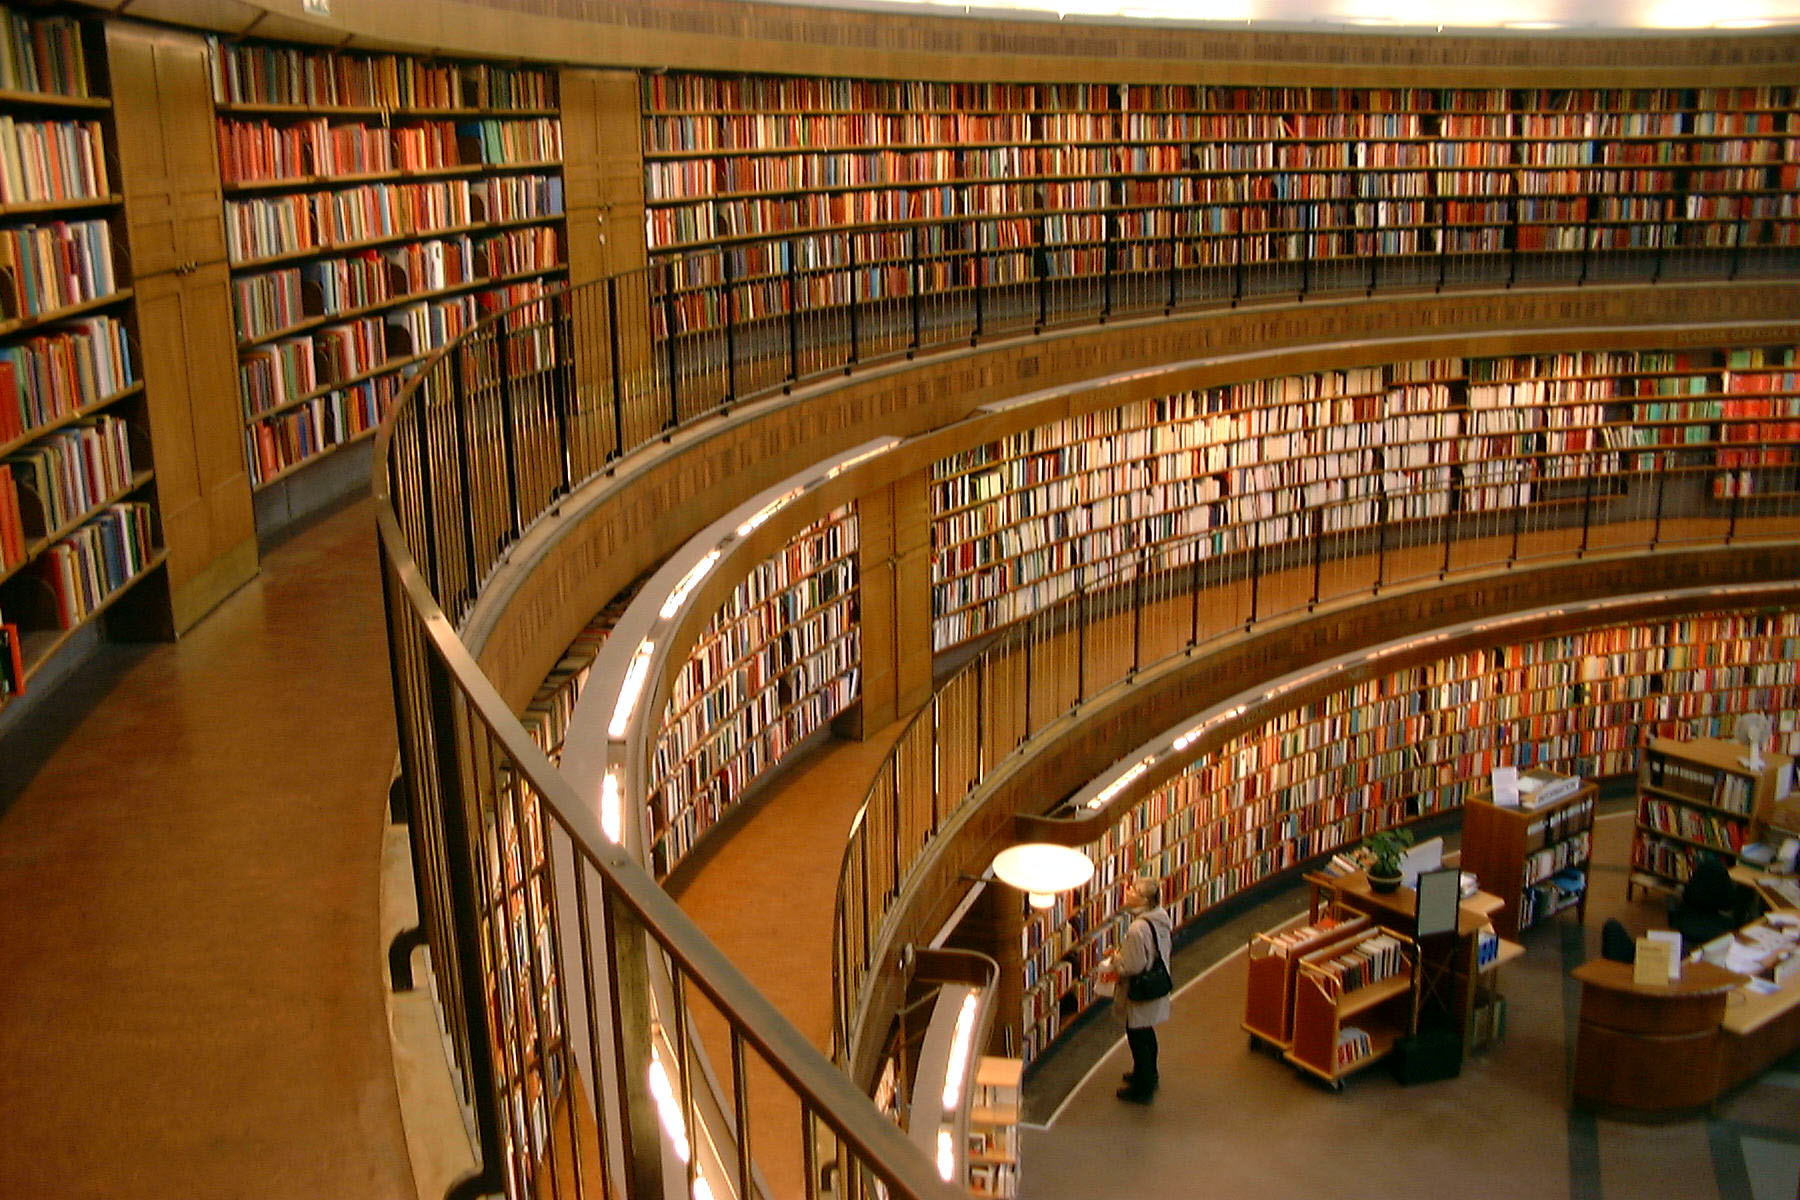
\includegraphics[width=0.9\linewidth]{images/library.jpg}\\
		\hspace*{15pt}\hbox{\scriptsize Image By:\thinspace{\itshape Marcus Hansson}}
		% https://commons.wikimedia.org/wiki/File:Interior_view_of_Stockholm_Public_Library.jpg
	\end{center}
		\column{0.455\linewidth}
			\begin{itemize}
			\item How do you look for books in a library? Say for instance you look for ``To kill a mockingbird'' by Harper Lee.
				\item You see ``Split second'' by David Baldacci and you need to look further down the shelf.
					
				\item You see ``The Amber Spyglass'' by Philip Pullman and you need to go back\dots
					
				\item Let's formalise that idea!
			\end{itemize}
	\end{columns}
\end{frame}

%%%%%%%%%%%%%%%%%%%%%%%%%%%%%%%%%%%%%%%%%%%%%%%%%%%%%%%%%%%%%%%%%%%%%%
\begin{frame}
	\frametitle{Déjà Vu all over again?}
	
			A recursive function is a function that calls itself.
		
		\begin{columns}
			\column{0.455\linewidth}
				For instance for Fibonacci:
				\begin{align*}
					F(1) &= 1 \\
					F(2) &= 1 \\
					F(n) &= F(n-1) + F(n-2) \text{ if $n > 2$}\\
				\end{align*}
			\column{0.455\linewidth}
			
		\lstinputlisting{src/fib.py}
				
		\end{columns}
\end{frame}

%%%%%%%%%%%%%%%%%%%%%%%%%%%%%%%%%%%%%%%%%%%%%%%%%%%%%%%%%%%%%%%%%%%%%%
\begin{frame}
	\frametitle{Binary Search}

			\begin{itemize}
			\item Given a sorted list $L$, determine if it contains an item with value $v$.
			\item Example: Sorted names:
			\begin{itemize}
			\item \texttt{L = [Angelova, Chong, Hugtenburg, Sijm, van den Akker]}
			\item Does it contain \texttt{Sijm}?
			\item Answer: Yes!
			\end{itemize}

			\item \alert{But how do we get there?}
			\item Remember that \texttt{in} from Python takes $\Theta(n)$ time. We want to improve on that!
		\end{itemize}	
\end{frame}

%%%%%%%%%%%%%%%%%%%%%%%%%%%%%%%%%%%%%%%%%%%%%%%%%%%%%%%%%%%%%%%%%%%%%%
\begin{frame}
	\frametitle{Binary search}
	
		Let's build this algorithm:
		
			\begin{columns}[t]
					
				\column{0.455\linewidth}
		\begin{itemize}
\item If the list is empty, return false
		\item Otherwise\dots Take the middle element of the list with index \texttt{m}, with value $x$.
		\item If $x = v$, return true.
		
		\item If $x > v$, return binary search in \texttt{L[:m]}.{start looking in the left{\_\_\_} side of the list.}
		\item If $x < v$, return binary search in \texttt{L[m+1:]}.{start looking in the right{\_\_\_} side of the list.}
		\end{itemize}
				\column{0.605\linewidth}

			\lstinputlisting{src/binary-search.py}	

			\end{columns}


\end{frame}

%%%%%%%%%%%%%%%%%%%%%%%%%%%%%%%%%%%%%%%%%%%%%%%%%%%%%%%%%%%%%%%%%%%%%%
\begin{frame}
	\frametitle{Binary search}

Filling in the blanks:

				What should we put on the blanks?
				
				\begin{itemize}
					\item `left' on line 3 and `left' on line 4. 
					\item `left' on line 3 and `right' on line 4. 
					\item `right' on line 3 and `left' on line 4. 
					\item `right' on line 3 and `right' on line 4. 
					\item I don't know.
				\end{itemize}	

Pseudocode:
				The above is what some might call \textit{pseudocode}. A natural language description of our program.			

				But just on the board, rather than in the slides.

\end{frame}

%%%%%%%%%%%%%%%%%%%%%%%%%%%%%%%%%%%%%%%%%%%%%%%%%%%%%%%%%%%%%%%%%%%%%%
\begin{frame}
	\frametitle{So how well does this do?}

Reminder: 			Our time to beat is the Python built-in \texttt{in} operator that requires $\Theta(n)$ time!

		\begin{columns}
			\column{0.605\linewidth}
				\lstinputlisting{src/binary-search.py}	
			\column{0.405\linewidth}
			
				\begin{itemize}
					\item What is the runtime of this function? 
					\item Try to formulate a recursive $T(n)$, where $n$ is \texttt{len(L)}.
					\item $T(0) = c_0$ for lines 5 and 6.
					\item $T(n) = T(\lfloor n/2 \rfloor) + c_1 + c_2n$ for lines 8 through 15.
			\end{itemize}
		\end{columns}
\end{frame}

%%%%%%%%%%%%%%%%%%%%%%%%%%%%%%%%%%%%%%%%%%%%%%%%%%%%%%%%%%%%%%%%%%%%%%
\begin{frame}
	\frametitle{So how well does this do? In terms of space $S(n)$}

		\begin{columns}
			\column{0.605\linewidth}
			\lstinputlisting{src/binary-search.py}	
			\column{0.405\linewidth}
				\begin{itemize}
					\item What is the runtime of this function? 
					\item Try to formulate a recursive $S(n)$, where $n$ is \texttt{len(L)}.
					\item $S(0) = c_0$ for lines 5 and 6.\\
					\item $S(n) = S(\lfloor n/2 \rfloor) + c_1 + c_2n$ for lines 8 through 15.
			\end{itemize}
		\end{columns}
\end{frame}

%%%%%%%%%%%%%%%%%%%%%%%%%%%%%%%%%%%%%%%%%%%%%%%%%%%%%%%%%%%%%%%%%%%%%%
\begin{frame}
	\frametitle{No improvements}
Reminder:
			Our time to beat is the Python built-in \texttt{in} operator that requires $\Theta(n)$ time!

Making it strictly better:
				\begin{itemize}
					\item This is still $O(n)$ at least... Because we make copies of the list in lines 13 and 14.
					\item How about we two more parameters: lowest index, largest index instead of a copy of half of the list.
					\item Now we only have $T(n) = T(n/2) + c_1$.
		\end{itemize}	
\end{frame}

%%%%%%%%%%%%%%%%%%%%%%%%%%%%%%%%%%%%%%%%%%%%%%%%%%%%%%%%%%%%%%%%%%%%%%
\begin{frame}
	\frametitle{How do we solve this?}

				\begin{itemize}
					\item Recurrence Equations: How do we get to $O(...)$ now?
	
					\item Repeated unfolding:
				\begin{itemize}
					\item $T(n) = T(n/2) +c_1$, so $T(n/2) = T(n/4) + c_1$.
					\item Substituting this, we get: $T(n) = T(n/4) + 2c_1$.
		\end{itemize}	
					
	\end{itemize}
	
As a computer scientist \ldots:
		To make the math a little `cleaner' we will assume $n = 2^m$ for some integer $m \geq 0$.	
\end{frame}

%%%%%%%%%%%%%%%%%%%%%%%%%%%%%%%%%%%%%%%%%%%%%%%%%%%%%%%%%%%%%%%%%%%%%%
\begin{frame}
	\frametitle{Solving it: getting a closed form}

	Repeated unfolding:
	\begin{align*}
		T(n) &= T(\lfloor n/2 \rfloor) + c_1\\
				 &= T(\lfloor n/4 \rfloor) + 2c_1\\
				 &= T(\lfloor n/8 \rfloor) + 3c_1\\
				 &= T(\lfloor n/2^k \rfloor) + kc_1\\
		\intertext{Take $k= \log_2(n+1)$ to get to $T(0)$}
		     &= T(\lfloor n/2^{\log_2(n+1)} \rfloor) + c_1\log_2(n+1)\\
				 &= T(0) + c_1\log_2(n+1)\\
				 &= c_0 + c_1\log_2(n+1)
	\end{align*}
\end{frame}

%%%%%%%%%%%%%%%%%%%%%%%%%%%%%%%%%%%%%%%%%%%%%%%%%%%%%%%%%%%%%%%%%%%%%%
\begin{frame}
	\frametitle{Confirming our `repeated unfolding'}
				\begin{itemize}
					\item How do we know this `guess' is correct?	
					\item Induction! (Let's see what you think of my idea of induction ;))
	\end{itemize}
\end{frame}

%%%%%%%%%%%%%%%%%%%%%%%%%%%%%%%%%%%%%%%%%%%%%%%%%%%%%%%%%%%%%%%%%%%%%%
\begin{frame}
	\frametitle{Proof by induction}

For powers of 2:

	\begin{proof}
		To prove: $T(n) = c_0 + c_1 \log_2(n)$ for $T(n)= \begin{cases}
			c_0 & \text{ if n = 1}\\
			T(n/2) + c_1 & \text{ else}
		\end{cases}$.	\\
		Base case ($n=0$): $T(0) = c_0 = c_0 + c_1 \cdot 0 = c_0 + c_1\log_2(0+1)$.\\
		Inductive case:
		Assume for arbitrary $k$: $T(k) = c_0 + c_1 \log_2(k+1)$. (IH)\\

		\begin{align*}
			T(2k) &= T(2k/2) + c_1\\
					 &= T(k) + c_1\\
					 &=_\text{\small IH} c_0 + c_1\log_2(k+1) + c_1\\
					 &= c_0 + c_1(\log_2(k+1) + \log_2(2))\\
					 &= c_0 + c_1(\log_2(2(k+1)))
		\end{align*}
		Since $k$ was arbitrarily chosen, it holds for all $n \geq 0$.
	\end{proof}
\end{frame}

%%%%%%%%%%%%%%%%%%%%%%%%%%%%%%%%%%%%%%%%%%%%%%%%%%%%%%%%%%%%%%%%%%%%%%
\begin{frame}
	\frametitle{So \ldots}

				\begin{itemize}
					\item Searching in an unsorted list: $O(n)$.
					\item Searching in an sorted list: $O(\log(n))$.
					\item Does that mean we should always sort our list?
		\end{itemize}	
\end{frame}
	% %%%%%%%%%%%%%%%%%%%%%%%%%%%%%%%%%%%%%%%%%%%%%%%%%%%%%%%%%%%%%%%%%%%%%%
\begin{frame}[fragile]\frametitle{}
\begin{center}
{\Large Sorting}
\end{center}

\end{frame}

%%%%%%%%%%%%%%%%%%%%%%%%%%%%%%%%%%%%%%%%%%%%%%%%%%%%%%%%%%%%%%%%%%%%%%
\begin{frame}
	\frametitle{BogoSort}
			The easiest form of sorting: Just try all permutations of the list.
		
Time complexity?:
			\begin{itemize}
				\item $\Theta(n)$
				\item $\Theta(n^2)$
				\item $\Theta(2^n)$
				\item $\Theta(n^n)$
				\item $\Theta(n!)$
				\item I don't know
			\end{itemize}
\end{frame}

%%%%%%%%%%%%%%%%%%%%%%%%%%%%%%%%%%%%%%%%%%%%%%%%%%%%%%%%%%%%%%%%%%%%%%
\begin{frame}
	\frametitle{Some questions and answers}
	Some observations and questions.
	\begin{itemize}
		\item The solution space is huge: $n!$ for $n$ items.
			
		\item The use case is not uncommon, so we hope/look for an efficient (polynomial time) algorithm.
			
		\item Humans have a lot of experience sorting items, can we use those strategies?
			
		\item Or are there methods that computers excel at, that would be terrible for humans?
	\end{itemize}

	\begin{itemize}
		\item There are polynomial time algorithms,
			
		\item We can translate our own methods,
		\item But computers can definitely do better.
	\end{itemize}
\end{frame}

%%%%%%%%%%%%%%%%%%%%%%%%%%%%%%%%%%%%%%%%%%%%%%%%%%%%%%%%%%%%%%%%%%%%%%
\begin{frame}
	\frametitle{Use case?}
		What do we use sorting for?
	
Many things!
		\begin{itemize}
			\item Books in the library.
			\item Exams for an exam review.
			\item Closest pair of points.
			\item Convex hulls.
			\item Efficient look-ups in lists that do not change.
			\item And many many more (see also later lectures in graph algorithms).
		\end{itemize}	
\end{frame}

%%%%%%%%%%%%%%%%%%%%%%%%%%%%%%%%%%%%%%%%%%%%%%%%%%%%%%%%%%%%%%%%%%%%%%
\begin{frame}[fragile]\frametitle{}
\begin{center}
{\Large Bubble Sort}
\end{center}

\end{frame}


%%%%%%%%%%%%%%%%%%%%%%%%%%%%%%%%%%%%%%%%%%%%%%%%%%%%%%%%%%%%%%%%%%%%%%
\begin{frame}[fragile]
	\frametitle{Bubble sort}
	
Your algorithm:
				\begin{lstlisting}
					While $v_i > v_{i+1}$ for some $i$
						State Switch them around.	
					EndWhile
				\end{lstlisting}
			
			\begin{center}
			\begin{tikzpicture}[scale=0.85, transform shape]
	\only<3>{
		\foreach \x/\val in {0/1,1/20,2/42,3/22,4/17}{
			\node[draw,rectangle, fill=gray!10, minimum size =1cm] (c) at (\x,0) {\val};
		}
	}
	\only<4>{
		\foreach \x/\val/\col in {0/1/green,1/20/green,2/42/black,3/22/black,4/17/black}{
			\node[draw=\col,rectangle, fill=\col!10, minimum size =1cm] (c) at (\x,0) {\val};
		}
	}
	\only<5>{
		\foreach \x/\val/\col in {0/1/black,1/20/green,2/42/green,3/22/black,4/17/black}{
			\node[draw=\col,rectangle, fill=\col!10, minimum size =1cm] (c) at (\x,0) {\val};
		}
	}
	\only<6>{
		\foreach \x/\val/\col in {0/1/black,1/20/black,2/42/red,3/22/red,4/17/black}{
			\node[draw=\col,rectangle, fill=\col!10, minimum size =1cm] (c) at (\x,0) {\val};
		}
	}
	\only<7>{
		\foreach \x/\val/\col in {0/1/black,1/20/black,2/22/green,3/42/green,4/17/black}{
			\node[draw=\col,rectangle, fill=\col!10, minimum size =1cm] (c) at (\x,0) {\val};
		}
	}
	\only<8>{
		\foreach \x/\val/\col in {0/1/black,1/20/black,2/22/black,3/42/red,4/17/red}{
			\node[draw=\col,rectangle, fill=\col!10, minimum size =1cm] (c) at (\x,0) {\val};
		}
	}
	\only<9>{
		\foreach \x/\val/\col in {0/1/black,1/20/black,2/22/black,3/17/green,4/42/green}{
			\node[draw=\col,rectangle, fill=\col!10, minimum size =1cm] (c) at (\x,0) {\val};
		}
	}
	\only<10>{
		\foreach \x/\val/\col in {0/1/green,1/20/green,2/22/black,3/17/black,4/42/black}{
			\node[draw=\col,rectangle, fill=\col!10, minimum size =1cm] (c) at (\x,0) {\val};
		}
	}
	\only<11>{
		\foreach \x/\val/\col in {0/1/black,1/20/green,2/22/green,3/17/black,4/42/black}{
			\node[draw=\col,rectangle, fill=\col!10, minimum size =1cm] (c) at (\x,0) {\val};
		}
	}
	\only<12>{
		\foreach \x/\val/\col in {0/1/black,1/20/black,2/22/red,3/17/red,4/42/black}{
			\node[draw=\col,rectangle, fill=\col!10, minimum size =1cm] (c) at (\x,0) {\val};
		}
	}
	\only<13>{
		\foreach \x/\val/\col in {0/1/black,1/20/black,2/17/green,3/22/green,4/42/black}{
			\node[draw=\col,rectangle, fill=\col!10, minimum size =1cm] (c) at (\x,0) {\val};
		}
	}
	\only<14>{
		\foreach \x/\val/\col in {0/1/black,1/20/black,2/17/black,3/22/green,4/42/green}{
			\node[draw=\col,rectangle, fill=\col!10, minimum size =1cm] (c) at (\x,0) {\val};
		}
	}
	\only<15>{
		\foreach \x/\val/\col in {0/1/green,1/20/green,2/17/black,3/22/black,4/42/black}{
			\node[draw=\col,rectangle, fill=\col!10, minimum size =1cm] (c) at (\x,0) {\val};
		}
	}
	\only<16>{
		\foreach \x/\val/\col in {0/1/black,1/20/red,2/17/red,3/22/black,4/42/black}{
			\node[draw=\col,rectangle, fill=\col!10, minimum size =1cm] (c) at (\x,0) {\val};
		}
	}
	\only<17>{
		\foreach \x/\val/\col in {0/1/black,1/17/green,2/20/green,3/22/black,4/42/black}{
			\node[draw=\col,rectangle, fill=\col!10, minimum size =1cm] (c) at (\x,0) {\val};
		}
	}
	\only<18>{
		\foreach \x/\val/\col in {0/1/black,1/17/black,2/20/green,3/22/green,4/42/black}{
			\node[draw=\col,rectangle, fill=\col!10, minimum size =1cm] (c) at (\x,0) {\val};
		}
	}
	\only<19>{
		\foreach \x/\val/\col in {0/1/black,1/17/black,2/20/black,3/22/green,4/42/green}{
			\node[draw=\col,rectangle, fill=\col!10, minimum size =1cm] (c) at (\x,0) {\val};
		}
	}
	\only<20>{
		\foreach \x/\val/\col in {0/1/green,1/17/green,2/20/black,3/22/black,4/42/black}{
			\node[draw=\col,rectangle, fill=\col!10, minimum size =1cm] (c) at (\x,0) {\val};
		}
	}
	\only<21>{
		\foreach \x/\val/\col in {0/1/black,1/17/green,2/20/green,3/22/black,4/42/black}{
			\node[draw=\col,rectangle, fill=\col!10, minimum size =1cm] (c) at (\x,0) {\val};
		}
	}
	\only<22>{
		\foreach \x/\val/\col in {0/1/black,1/17/black,2/20/green,3/22/green,4/42/black}{
			\node[draw=\col,rectangle, fill=\col!10, minimum size =1cm] (c) at (\x,0) {\val};
		}
	}
	\only<23->{
		\foreach \x/\val/\col in {0/1/black,1/17/black,2/20/black,3/22/green,4/42/green}{
			\node[draw=\col,rectangle, fill=\col!10, minimum size =1cm] (c) at (\x,0) {\val};
		}
	}
\end{tikzpicture}

			\end{center}

				So how many inversions can there be?
				\begin{itemize}
					\item $\Theta(n)$
					\item $\Theta(n^2)$
					\item $\Theta(n^n)$
					\item $\Theta(n!)$
				\end{itemize}
\end{frame}

%%%%%%%%%%%%%%%%%%%%%%%%%%%%%%%%%%%%%%%%%%%%%%%%%%%%%%%%%%%%%%%%%%%%%%
\begin{frame}
	\frametitle{The number of inversions}

		Consider a list in reverse order:
		\begin{itemize}
			\item The first element is wrong compared to all others: $n-1$ inversions.
		
			\item The second is also wrong with all the ones that come after it: $n-2$ extra inversions.
			\item \ldots
		
			\item The one-but last one is also wrong with the last one: $1$ inversion
		
			\item So $\Theta(n^2)$ inversion!
		\end{itemize}
\end{frame}

%%%%%%%%%%%%%%%%%%%%%%%%%%%%%%%%%%%%%%%%%%%%%%%%%%%%%%%%%%%%%%%%%%%%%%
\begin{frame}
	\frametitle{To summarise in code}
	\begin{columns}[T]
		\column{0.565\linewidth}
	\lstinputlisting{src/bs.py}
		\column{0.455\linewidth}
Pros and Cons?:
			What are the pros and cons of bubblesort? Hint: remember I told you it was slow!
	\end{columns}
\end{frame}

%%%%%%%%%%%%%%%%%%%%%%%%%%%%%%%%%%%%%%%%%%%%%%%%%%%%%%%%%%%%%%%%%%%%%%
\begin{frame}
	\frametitle{Bubblesort: Pros and Cons}

			While there are inversions: fix them.
Pros:
			\begin{itemize}
				\item Great in a distributed setting, with autonomous agents (like students in a lecture hall).
				\item When implemented as: ``continue while there are inversion'' can terminate after one iteration over a
					sorted list! 
				\item Easiest to implement.
			\end{itemize}


Cons:
			\begin{itemize}
				\item Terribly slow! (Often still slower than other $\Theta(n^2)$ algorithms we will see later)
			\end{itemize}
\end{frame}

%%%%%%%%%%%%%%%%%%%%%%%%%%%%%%%%%%%%%%%%%%%%%%%%%%%%%%%%%%%%%%%%%%%%%%
\begin{frame}[fragile]\frametitle{}
\begin{center}
{\Large Bucket Sort}
\end{center}

\end{frame}

%%%%%%%%%%%%%%%%%%%%%%%%%%%%%%%%%%%%%%%%%%%%%%%%%%%%%%%%%%%%%%%%%%%%%%
\begin{frame}
	\frametitle{Bucket Sort}
The Stephen Tatlock algorithm\dots 

			\begin{itemize}
				\item Sort the items into buckets (e.g. based on first letter of last name).
					
				\item Sort every bucket.
					
				\item Concatenate all buckets together.
			\end{itemize}
		

			Why should we use this?
		
			\begin{itemize}
				\item Great for parallelisation!
				\item Great for humans (sorting a bucket can be done using a different algorithm, everyone can pick their own
					favourite).
				\item Average case analysis is interesting for this algorithm (and gets us to something close to linear time for
					average case).
			\end{itemize}
\end{frame}

%%%%%%%%%%%%%%%%%%%%%%%%%%%%%%%%%%%%%%%%%%%%%%%%%%%%%%%%%%%%%%%%%%%%%%
\begin{frame}[fragile]\frametitle{}
\begin{center}
{\Large Selection Sort}
\end{center}

\end{frame}

%%%%%%%%%%%%%%%%%%%%%%%%%%%%%%%%%%%%%%%%%%%%%%%%%%%%%%%%%%%%%%%%%%%%%%
\begin{frame}
	\frametitle{Selection Sort}
			\begin{itemize}
				\item The smallest of variations \ldots
				\item Rather than shifting every element to it's correct place\dots
				\item We instead repeatedly search for the smallest element and put it at the end of our sorted list/sorted part.
			\end{itemize}
				
	\begin{center}
	\section{Selection Sort}
\label{sec:selection_sort}

\begin{frame}
	\frametitle{Selection Sort}
		\begin{block}{The smallest of variations...}
			Rather than shifting every element to it's correct place\dots\\
			\pause
			We instead repeatedly search for the smallest element and put it at the end of our sorted list/sorted part.
		\end{block}	
	\begin{center}
	\input{figures/tikz/selectionsort.tex}
	\end{center}
\end{frame}

\begin{frame}
	\frametitle{Implementation}
	\begin{exampleblock}{Time Complexity}
		Still $\Theta(n^2)$ as we need to find the minimum $O(n)$ times, which takes $O(n)$ time.
		\end{exampleblock}	
	\begin{alertblock}{See next week's homework}
		You will tell me next week ;)
	\end{alertblock}	
\end{frame}

\begin{frame}
	\frametitle{In-place sorting algorithms}
	\framesubtitle{I'm not going anywhere!}

	\begin{itemize}
		\item The sorting algorithms we have seen so-far are \alert{in-place} sorting algorithms.
			\pause
		\item They take a list and modify that list to become sorted.
			\pause
		\item Of course we can also make them not in-place, by first making a copy of the list and sorting that.
			\pause
		\item But after the break (when we discuss merge sort) we will see an example of an algorithm that is easier to make
			not in-place.
	\end{itemize}
\end{frame}



	\end{center}
\end{frame}

%%%%%%%%%%%%%%%%%%%%%%%%%%%%%%%%%%%%%%%%%%%%%%%%%%%%%%%%%%%%%%%%%%%%%%
\begin{frame}
	\frametitle{Implementation}
Time Complexity: 		Still $\Theta(n^2)$ as we need to find the minimum $O(n)$ times, which takes $O(n)$ time.
	
\end{frame}

%%%%%%%%%%%%%%%%%%%%%%%%%%%%%%%%%%%%%%%%%%%%%%%%%%%%%%%%%%%%%%%%%%%%%%

\begin{frame}
	\frametitle{In-place sorting algorithms}

	\begin{itemize}
		\item The sorting algorithms we have seen so-far are \alert{in-place} sorting algorithms.
			
		\item They take a list and modify that list to become sorted.
			
		\item Of course we can also make them not in-place, by first making a copy of the list and sorting that.
			
		\item But after the break (when we discuss merge sort) we will see an example of an algorithm that is easier to make
			not in-place.
	\end{itemize}
\end{frame}

%%%%%%%%%%%%%%%%%%%%%%%%%%%%%%%%%%%%%%%%%%%%%%%%%%%%%%%%%%%%%%%%%%%%%%
\begin{frame}[fragile]\frametitle{}
\begin{center}
{\Large Insertion Sort}
\end{center}

\end{frame}

%%%%%%%%%%%%%%%%%%%%%%%%%%%%%%%%%%%%%%%%%%%%%%%%%%%%%%%%%%%%%%%%%%%%%%
\begin{frame}
	\frametitle{Insertion Sort}

			The main idea:
			\begin{itemize}
				\item We build the list, step by step.
					
				\item We keep our intermediate result sorted.
					
				\item At every step, we insert the next element into the right place.
					
				\item This means we need to shift over (worst-case) $n$ elements for every element we insert...
					
				\item So in total $\Theta(n^2)$ time.
			\end{itemize}

\end{frame}

%%%%%%%%%%%%%%%%%%%%%%%%%%%%%%%%%%%%%%%%%%%%%%%%%%%%%%%%%%%%%%%%%%%%%%
\begin{frame}[fragile]
	\frametitle{Insertion Sort}
	
	\begin{lstlisting}
		State $i gets 1$ Comment {The first element forms a sorted list on it's own}
		
		While $i < \texttt{len}(l)$
		State $j gets i$
		
		While $j > 0$ and $v_{j-1} < v_{j}$ 
			State swap $v_j$ and $v_{j-1}$	
			State $j gets j -1$
		EndWhile
		
		State $i gets i+1$
		EndWhile
	\end{lstlisting}
	
	\begin{center}
	\section{Insertion Sort}
\label{sec:insertion_sort}

\begin{frame}
	\frametitle{Insertion sort}
	\begin{center}
		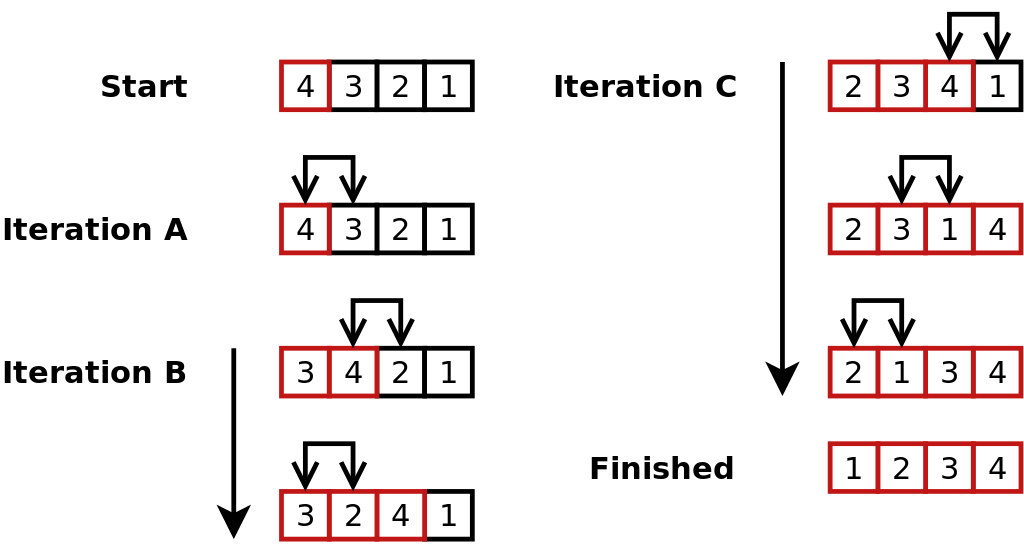
\includegraphics[width=0.8\textwidth]{figures/insertionsort.png}\\
		\hspace*{15pt}\hbox{\scriptsize Image By:\thinspace{\itshape MrDrBob}}
		% https://commons.wikimedia.org/wiki/File:Insertion-sort.svg
	\end{center}
\end{frame}

\begin{frame}
	\frametitle{Insertion Sort}
	\framesubtitle{How does that work?}
		\begin{block}{Insertion Sort}
			The main idea:
			\begin{itemize}
				\item We build the list, step by step.
					\pause
				\item We keep our intermediate result sorted.
					\pause
				\item At every step, we insert the next element into the right place.
					\pause
				\item This means we need to shift over (worst-case) $n$ elements for every element we insert...
					\pause
				\item So in total $\Theta(n^2)$ time.
			\end{itemize}
		\end{block}
\end{frame}

\begin{frame}
	\frametitle{Insertion Sort}
	\begin{algorithmic}
		\State $i \gets 1$ \Comment{The first element forms a sorted list on it's own}
		\pause
		\While{$i < \texttt{len}(l)$}
		\State $j \gets i$
		\pause
		\While{$j > 0$ and $v_{j-1} < v_{j}$}
			\State swap $v_j$ and $v_{j-1}$	
			\State $j \gets j -1$
		\EndWhile
		\pause
		\State $i \gets i+1$
		\EndWhile
	\end{algorithmic}
	\pause
	\begin{center}
	\input{figures/tikz/insertionsort.tex}
	\end{center}
\end{frame}

\begin{frame}
	\frametitle{Would you like some sausages with your cheese?}
	\begin{columns}
		\column{0.455\textwidth}
		\begin{algorithmic}
			\State $i \gets 1$ 
			\While{$i < \texttt{len}(l)$}
			\State $j \gets i$
			\While{$j > 0$ and $v_j < v_{j-1}$}
			\State swap $v_j$ and $v_{j-1}$	
			\State $j \gets j -1$
			\EndWhile
			\State $i \gets i+1$
			\EndWhile
		\end{algorithmic}
		\column{0.455\textwidth}
		\begin{questionblock}{Run time}
			What instance of a list would give the worst performance here?	
		\end{questionblock}
		\pause
		\begin{answerblock}{Again!?}
			Once again it is the reverse list, where every item needs to be moved to the front requiring most swaps.
		\end{answerblock}
		\pause
			\begin{block}{So...}
				The run time is still $\Theta(n^2)$.
			\end{block}	
	\end{columns}

	
\end{frame}

\begin{frame}
	\frametitle{Implementation to summarise}
	
		\begin{alertblock}{See you tomorrow!}
			We will implement this tomorrow :)
		\end{alertblock}	
\end{frame}

\begin{frame}
	\frametitle{Insertion Sort: Pros and Cons}
		\begin{block}{Insertion Sort}
			Repeatedly insert the next item in the correct place in a sorted list.
		\end{block}	
		\begin{exampleblock}{Pros}
			\begin{itemize}
				\item `Easy' algorithm to implement.
				\item Good performance for an $O(n^2)$ algorithm.
			\end{itemize}
		\end{exampleblock}	
		\begin{alertblock}{Cons}
			\begin{itemize}
				\item Still not as fast as comparison-based sorting algorithms can be.
			\end{itemize}
		\end{alertblock}	
	
\end{frame}

	\end{center}
\end{frame}

%%%%%%%%%%%%%%%%%%%%%%%%%%%%%%%%%%%%%%%%%%%%%%%%%%%%%%%%%%%%%%%%%%%%%%
\begin{frame}[fragile]
	\frametitle{Would you like some sausages with your cheese?}
	
	\begin{columns}[T]
		\column{0.455\linewidth}
		\begin{lstlisting}
			State $i \gets 1$ 
			While $i < \texttt{len}(l)$
			State $j \gets i$
			While $j > 0$ and $v_j < v_{j-1}$
			State swap $v_j$ and $v_{j-1}$	
			State $j \gets j -1$
			EndWhile
			State $i \gets i+1$
			EndWhile
		\end{lstlisting}
		\column{0.455\linewidth}
			\begin{itemize}
				\item Run time:		What instance of a list would give the worst performance here?	
				\item Once again it is the reverse list, where every item needs to be moved to the front requiring most swaps.
				\item The run time is still $\Theta(n^2)$.
			\end{itemize}	
	\end{columns}
\end{frame}

%%%%%%%%%%%%%%%%%%%%%%%%%%%%%%%%%%%%%%%%%%%%%%%%%%%%%%%%%%%%%%%%%%%%%%
\begin{frame}
	\frametitle{Insertion Sort: Pros and Cons}
			\begin{itemize}
				\item Insertion Sort:	Repeatedly insert the next item in the correct place in a sorted list.
				\item Pros:
			\begin{itemize}
				\item `Easy' algorithm to implement.
				\item Good performance for an $O(n^2)$ algorithm.
			\end{itemize}
				\item Cons:
			\begin{itemize}
				\item Still not as fast as comparison-based sorting algorithms can be.
			\end{itemize}
		\end{itemize}	
	
\end{frame}

%%%%%%%%%%%%%%%%%%%%%%%%%%%%%%%%%%%%%%%%%%%%%%%%%%%%%%%%%%%%%%%%%%%%%%
\begin{frame}[fragile]\frametitle{}
\begin{center}
{\Large Merge Sort}
\end{center}

\end{frame}

%%%%%%%%%%%%%%%%%%%%%%%%%%%%%%%%%%%%%%%%%%%%%%%%%%%%%%%%%%%%%%%%%%%%%%
\begin{frame}
	\frametitle{Merge Sort}
			\begin{itemize}
				\item A recursive sorting algorithm.
				\item It splits the list into two, sorts each half, then combines the results.

				\item Not great for humans: this algorithm is not the easiest for humans to perform.
				\item Great for computers:	But computers do excellent at it!
	\end{itemize}	
\end{frame}

%%%%%%%%%%%%%%%%%%%%%%%%%%%%%%%%%%%%%%%%%%%%%%%%%%%%%%%%%%%%%%%%%%%%%%
\begin{frame}[fragile]
	\frametitle{The idea}

			The algorithm:
		\begin{lstlisting}
			Function{MergeSort}{xs}
				If{len(xs) $< 2$}	
					State Return xs
				EndIf
			
				State leftHalf $gets$ Call{MergeSort}{the first half of the list}
				State rightHalf $gets$ Call{MergeSort}{the second half of the list}
			
				State result $gets []$, $i gets 0$, $j gets 0$
				While{$i < $ len(leftHalf) and $j < $ len(rightHalf)}
					State\alert{Something goes here}
					State\alert{Update $i$ and $j$ accordingly.}

				:
			EndFunction
		\end{lstlisting}
		

\end{frame}

%%%%%%%%%%%%%%%%%%%%%%%%%%%%%%%%%%%%%%%%%%%%%%%%%%%%%%%%%%%%%%%%%%%%%%
\begin{frame}[fragile]
	\frametitle{The idea}

			The algorithm:
		\begin{lstlisting}
			Function{MergeSort}{xs}
				:

				If{leftHalf[i] $<$ rightHalf[j]}
					State result.append(leftHalf[i]),  $i gets i + 1$
				Else
					State 
					State result.append(rightHalf[j]),  $j gets j + 1$
				EndIf
				State \alert{Something here?}
				While{$i < $ len(leftHalf)}
					State result.append(leftHalf[i]),  $i\gets i + 1$
				EndWhile
				While{$j < $ len(rightHalf)}
					State result.append(rightHalf[j]),  $j\gets j + 1$
				EndWhile
				State Return result
			EndFunction
		\end{lstlisting}
		
\end{frame}

%%%%%%%%%%%%%%%%%%%%%%%%%%%%%%%%%%%%%%%%%%%%%%%%%%%%%%%%%%%%%%%%%%%%%%
\begin{frame}[fragile]
	\frametitle{The idea}

		
			What do we do here?
				\begin{itemize}
					\item Compare leftHalf[0] with rightHalf[0]
					\item Compare leftHalf[i] with rightHalf[0]
					\item Compare leftHalf[0] with rightHalf[j]
					\item Compare leftHalf[i] with rightHalf[j]
				\end{itemize}
				What do we do here?
				\begin{itemize}
					\item Nothing, we're done
					\item Empty the remainder of the left half, then the right half.
					\item Empty the remainder of the right half, then the left half.
					\item Only one half can still have items left, empty that one.
				\end{itemize}
				You can see one con:		The algorithm is a bit more involved \ldots
				Is it better?: What is a tight bound on the run time?	Hint: you can use the master theorem!
\end{frame}

%%%%%%%%%%%%%%%%%%%%%%%%%%%%%%%%%%%%%%%%%%%%%%%%%%%%%%%%%%%%%%%%%%%%%%
\begin{frame}
	\frametitle{Merge sort run time}
				\begin{itemize}
					\item $T(0) = T(1) = c_0$ and $T(n) = 2T(n/2) + \Theta(n)$
					\item This gives $n^{\log_2(2)} = n$ leaves, and as $f(n) = \Theta(n)$ this makes this case 2 of the master method
					\item Thus $\Theta(n\log n)$ work! We improved!
					\item Worst-case instance?:
		What would be the worst type of list for this algorithm?
	
					\item There is none
					\item There is no worst-case instance, all of them take $\Theta(n \log n)$ time as we append $n$ items in $\log n$
		recursive calls in the recursion tree.
	\end{itemize}
\end{frame}

%%%%%%%%%%%%%%%%%%%%%%%%%%%%%%%%%%%%%%%%%%%%%%%%%%%%%%%%%%%%%%%%%%%%%%
\begin{frame}
	\frametitle{Merge sort: pros and cons}
	\begin{block}{Merge sort}
			Recursively split the list, sort and merge sorted lists.
		\end{block}	
		\begin{block}{Pros}
			\begin{itemize}
				\item Great in a distributed setting, as it can be parallelised!
				\item Great time complexity! $O(n\log n)$
			\end{itemize}
		\end{block}	
		\begin{block}{Cons}
			\begin{itemize}
				\item A bit harder to implement.
				\item Always takes $O(n \log n)$ even when only two items would have to be switched.
			\end{itemize}
		\end{block}	
\end{frame}

%%%%%%%%%%%%%%%%%%%%%%%%%%%%%%%%%%%%%%%%%%%%%%%%%%%%%%%%%%%%%%%%%%%%%%
\begin{frame}[fragile]\frametitle{}
\begin{center}
{\Large Quick Sort}
\end{center}

\end{frame}

%%%%%%%%%%%%%%%%%%%%%%%%%%%%%%%%%%%%%%%%%%%%%%%%%%%%%%%%%%%%%%%%%%%%%%
\begin{frame}
	\frametitle{Quicksort}
			\begin{itemize}
				\item A recursive sorting algorithm.
				\item It splits the list into two, sorts each half, then combines the results.
				\item That sounds exactly like mergesort!?
	\end{itemize}	
\end{frame}

%%%%%%%%%%%%%%%%%%%%%%%%%%%%%%%%%%%%%%%%%%%%%%%%%%%%%%%%%%%%%%%%%%%%%%
\begin{frame}[fragile]
	\frametitle{The idea}
		\begin{columns}[T]
			\column{0.705\linewidth}
			The algorithm:
		\begin{lstlisting}
			Function{Quicksort}{xs}
				If{len(xs) $< 2$}	
					State Return xs
				EndIf
				
				State pivot $gets$ some element from xs
				State left $gets$ everything smaller than pivot
				State right $gets$ everything larger than pivot
				State leftHalf $gets$ Call{Quicksort}{left}
				State rightHalf $gets$ Call{Quicksort}{right}
				
				State Return \alt<5->{leftHalf + pivot + rightHalf}{\dots}
			EndFunction
		\end{lstlisting}
		
			\column{0.305\linewidth}
			What do we do here?
				\begin{itemize}
					\item Merge the left and right half.
					\item Return left + right
					\item Return left + pivot + right
					\item Return right + pivot + left
				\end{itemize}
	
					What is the time complexity of this?\\
					Or rather, what does the worst case input look like?
		\end{columns}
\end{frame}

%%%%%%%%%%%%%%%%%%%%%%%%%%%%%%%%%%%%%%%%%%%%%%%%%%%%%%%%%%%%%%%%%%%%%%
\begin{frame}
	\frametitle{It depends!}
				\begin{itemize}
					\item Everything stands and falls by the choice of pivot.
					\item The first element:
		What is the worst input if we always take the first element as the pivot?
					\item 
					\begin{itemize}
						\item A sorted list
						\item The reverse of a sorted list
						\item A list that has the first $n/2$ elements sorted ascendingly and the second $n/2$ elements sorted descendingly.
					\end{itemize}
					\item This takes of only $1$ element every time, meaning we need $O(n^2)$ time.	
	\end{itemize}
\end{frame}

%%%%%%%%%%%%%%%%%%%%%%%%%%%%%%%%%%%%%%%%%%%%%%%%%%%%%%%%%%%%%%%%%%%%%%
\begin{frame}
	\frametitle{In practice}
	
Quick Sort in the real world:
			\begin{itemize}
				\item It is the most common sorting algorithm used.
				\item The implementations choose \textit{random} pivots.
					
				\item Worst-case this is still $O(n^2)$ of course.
					
				\item But with some fancy analysis (that we will not go into today, but maybe tomorrow ;)), we can show that
					this is $O(n \log n)$ in expectation (average case if you will).
					
				\item In practice this often outperforms merge sort significantly, especially when we make it in-place.
			\end{itemize}
\end{frame}

%%%%%%%%%%%%%%%%%%%%%%%%%%%%%%%%%%%%%%%%%%%%%%%%%%%%%%%%%%%%%%%%%%%%%%
\begin{frame}
	\frametitle{Quicksort: pros and cons}
			\begin{itemize}
				\item Recursively split the list in smaller and larger elements, sort and combine.
				\item Pros:
			\begin{itemize}
				\item Great time complexity for average case $O(n\log n)$
				\item Simpler to implement (and faster in most cases) than merge sort.
				\item Argument based on authority: the whole world uses it.
			\end{itemize}
				\item Cons:
			\begin{itemize}
				\item Still $O(n^2)$ if we are unlucky in choosing pivots.
			\end{itemize}
		\end{itemize}	
\end{frame}

%%%%%%%%%%%%%%%%%%%%%%%%%%%%%%%%%%%%%%%%%%%%%%%%%%%%%%%%%%%%%%%%%%%%%%
\begin{frame}[fragile]\frametitle{}
\begin{center}
{\Large Sorting Summary}
\end{center}

\end{frame}

%%%%%%%%%%%%%%%%%%%%%%%%%%%%%%%%%%%%%%%%%%%%%%%%%%%%%%%%%%%%%%%%%%%%%%
\begin{frame}
	\frametitle{Summary table}
	\begin{tabular}{r | c | c | c}
		\small
		Sorting method & Time & Main advantage & Main disadvantage \\
		\midrule
		Bubble Sort & $O(n^2)$ & Easy for humans! &  Very very very very slow \\
		Insertion Sort & $O(n^2)$ & Good for small lists &  Still quadratic time \\
		Selection Sort & $O(n^2)$ & Good for small lists &  Still quadratic time \\
		Merge Sort & $O(n \log n)$ & Faster than quadratic! &  Bad on `almost sorted lists' \\
		Quick Sort & $O(n \log n)$\footnote{in expectation} & Faster than merge sort &  Still worst-case quadratic\dots \\
	\end{tabular}
	\begin{itemize}
		\item We can mix Bucket Sort in with all this, by applying it first and then applying it (or one of the others) on
			the different buckets.
		\item Sorting algorithms can be in-place or not.
	\end{itemize}
\end{frame}

%%%%%%%%%%%%%%%%%%%%%%%%%%%%%%%%%%%%%%%%%%%%%%%%%%%%%%%%%%%%%%%%%%%%%%
\begin{frame}
	\frametitle{But wait!}
	
	\begin{itemize}
		\item Stable sorting: Didn't I also mention stable sorting yesterday?
		\item A sorting is stable if: in a list where if $k_i = k_j$ (where $k$ denotes the sorting key,
			e.g. age, or length) and $v_i$ comes for $v_j$ before sorting, then $v_i$ still comes before $v_j$ after sorting.
		\item Check for yourselves:
	\begin{itemize}
		\item Insertion sort is stable!
		\item Merge sort is not!
			\end{itemize}

			\end{itemize}	
\end{frame}
	% %%%%%%%%%%%%%%%%%%%%%%%%%%%%%%%%%%%%%%%%%%%%%%%%%%%%%%%%%%%%%%%%%%%%%%
\begin{frame}[fragile]\frametitle{}
\begin{center}
{\Large Computational Complexity}
\end{center}

\end{frame}

%%%%%%%%%%%%%%%%%%%%%%%%%%%%%%%%%%%%%%%%%%%%%%%%%%%%%%%%%%%%%%%%%%%%%%
\begin{frame}
	\frametitle{What does it do?, How fast does it do it?}

		
			\begin{itemize}
			\item What does the code compute?
			\item Sum of squares: \texttt{foo(n)} computes $\sum\limits_{i=0}^{n-1} i^2$
			\item How fast is it?
			\item Harder to answer:
			\item 1 second for $n=1000$.
			\item But what if $n$ changes?
			\item And what if we use another computer?
	\end{itemize}
	
		\lstinputlisting{src/for-loop.py}
	
\end{frame}

%%%%%%%%%%%%%%%%%%%%%%%%%%%%%%%%%%%%%%%%%%%%%%%%%%%%%%%%%%%%%%%%%%%%%%
\begin{frame}
	\frametitle{Why do we ask this?}

	\begin{columns}
		\column{0.455\textwidth}
			\begin{itemize}
			\item \lstinputlisting{src/for-loop.py}
			
			\item \lstinputlisting{src/nested-for-loop.py}
	\end{itemize}
			
		\column{0.455\textwidth}
		
			\begin{itemize}
			\item Comparing implementations: 	How can we compare \texttt{foo} and \texttt{bar}?
			\item By counting operations!
		\end{itemize}
	\end{columns}
\end{frame}

%%%%%%%%%%%%%%%%%%%%%%%%%%%%%%%%%%%%%%%%%%%%%%%%%%%%%%%%%%%%%%%%%%%%%%
\begin{frame}
	\frametitle{Counting operations}
	\begin{columns}
		\column{0.455\textwidth}
			\lstinputlisting{src/for-loop.py}
		\column{0.455\textwidth}
		
Counting operations:			How many operations happen when we call \texttt{foo(n)}?
			\begin{itemize}
				\item $2 + n$
				\item $2 + n + n$
				\item $3 + 2n + n-1$
				\item $4 + n + n + n + n-1$
			\end{itemize}
	\end{columns}
\end{frame}

%%%%%%%%%%%%%%%%%%%%%%%%%%%%%%%%%%%%%%%%%%%%%%%%%%%%%%%%%%%%%%%%%%%%%%
\begin{frame}
	\frametitle{Getting rid of those nasty constants}

	\begin{itemize}
		\item Observation: We do not care if it's is $2+n$ or even $3+2n$.
		\item The important part is that it \textit{scales with the input}.
			
		\item We call this the ``asymptotic run time complexity''.
	
		\item \lstinputlisting{src/for-loop.py}

		\item No more numbers:		We say this code has $c_0 + c_1n$ operations, where:
		\begin{itemize}
			\item $c_0$ is initialisation of $s$ on line 2 and the return statement on line 5.
			\item $c_1$ is the \texttt{range} function on line 3 and the multiplication and addition on line 4.
		\end{itemize}
	\end{itemize}
\end{frame}

%%%%%%%%%%%%%%%%%%%%%%%%%%%%%%%%%%%%%%%%%%%%%%%%%%%%%%%%%%%%%%%%%%%%%%
\begin{frame}
	\frametitle{Getting rid of those nasty constants}

	\begin{itemize}
		\item lstinputlisting{src/nested-for-loop.py}
		\item So what about here?:	How can we describe the number of operations here?	
		\item Quadratic time:
				We say this code has $c_0 + c_1n + c_2 n^2$ operations, where:
				\begin{itemize}
					\item $c_0$ is initialisation of $s$ on line 2 and the return statement on line 6.
					\item $c_1$ is the \texttt{range} function on line 3.
					\item $c_2$ is the \texttt{range} function on line 4 and the multiplication and addition on line 5.
				\end{itemize}
			\end{itemize}
\end{frame}

%%%%%%%%%%%%%%%%%%%%%%%%%%%%%%%%%%%%%%%%%%%%%%%%%%%%%%%%%%%%%%%%%%%%%%
\begin{frame}
	\frametitle{Some numbers!}
	
Differences in run time for	Different code snippets, all executed 1000 times.

		\hfill\\
		\begin{tabular}{c | c c c c c c c}
			\scriptsize
			Input size & constant & linear & quadratic & cubic & exponential & factorial\\
			\midrule
			
			1 & $<$10 ms & $<$10 ms & $<$10 ms & $<$10 ms & $<$10 ms & $<$10 ms\\
			2 & $<$10 ms & $<$10 ms & $<$10 ms & $<$10 ms & $<$10 ms & $<$10 ms\\
			
			5 & $<$10 ms & $<$10 ms & $<$10 ms & 36 ms & 40 ms & 210 ms\\
			
			7 & $<$10 ms & $<$10 ms & $<$10 ms & 49 ms & 50 ms & \alert{$>$3000 ms} \\
			
			10 & $<$10 ms & $<$10 ms & 23 ms & 78 ms & 84 ms & \alert{$>$3000 ms}\\
			
			100 & $<$10 ms & $<$10 ms & 284 ms & \alert{$>$3000 ms} & \alert{$>$3000 ms} & \alert{$>$3000 ms} \\
			
			1000 & $<$10 ms & 54 ms & \alert{$>$3000 ms} &\alert{$>$3000 ms} & \alert{$>$3000 ms} & \alert{$>$3000 ms} \\
			
			10000 & $<$10 ms &  \alert{$>$3000 ms} &\alert{$>$3000 ms} &\alert{$>$3000 ms} & \alert{$>$3000 ms} & \alert{$>$3000 ms} \\
		\end{tabular}
\end{frame}

%%%%%%%%%%%%%%%%%%%%%%%%%%%%%%%%%%%%%%%%%%%%%%%%%%%%%%%%%%%%%%%%%%%%%%
\begin{frame}
	\frametitle{Big-Oh notation}

	\begin{itemize}
		\item We care about what we call: ``asymptotic run time complexity''.
		\item We denote this using big-Oh, e.g.\ $f(n) = 3n + 2$ is $O(n)$.

		\item You (may?) have used big-Oh to a certain point before. E.g.\ as $n$ approaches $5$.
			
		\item In computer science we only think about when $n$ approaches $\infty$.
	\end{itemize}
\end{frame}

%%%%%%%%%%%%%%%%%%%%%%%%%%%%%%%%%%%%%%%%%%%%%%%%%%%%%%%%%%%%%%%%%%%%%%
\begin{frame}
	\frametitle{Formally}
	\begin{definition}[Big-Oh]
		A function $f(n)$ is $O(g(n))$ iff there is a positive real constant $c$ and a positive integer $n_0$ such that for
		all $n \geq n_0$ it holds that $f(n) \leq c g(n)$. In other words:\\
		$\exists c \in \mathbb{R}, \exists n_0 \in \mathbb{N} (c > 0 \wedge n_0 \geq 1 \wedge (\forall n \in \mathbb{N} (n
		\geq n_0 \to f(n) \leq cg(n))))$.
	\end{definition}
	
		Which of the following is/are true?
		\begin{itemize}
			\item $n^2$ is $O(n^3)$
			\item $8n^2$ is $O(n^2)$
			\item $16n^2 + 5n + 2$ is $O(n^2)$
			\item $16n^2 + 5n \log n$ is $O(n^2)$
			\item $16n^2\log n$ is $O(n^2)$
		\end{itemize}
\end{frame}

%%%%%%%%%%%%%%%%%%%%%%%%%%%%%%%%%%%%%%%%%%%%%%%%%%%%%%%%%%%%%%%%%%%%%%
\begin{frame}
	\frametitle{Let's prove that}

		Prove that $f(n) = 16n^2 + 5n + 2$ is $O(n^2)$.
	
	\begin{proof}
		To prove: $\exists c > 0, n_0 \geq 1$ such that $\forall n \geq n_0$ $16n^2 + 5n + 2 \leq cn^2$.\\
		
		Take $n_0 = 1$, now for all $n \in \mathbb{N}$ with $n \geq n_0$:
		\begin{align*}
			16n^2 + 5n + 2 &\leq 16n^2 + 5n^2 + 2n^2 \\
										 &= 23n^2
		\end{align*}
		So take $c=23$.
	\end{proof}
\end{frame}

%%%%%%%%%%%%%%%%%%%%%%%%%%%%%%%%%%%%%%%%%%%%%%%%%%%%%%%%%%%%%%%%%%%%%%
\begin{frame}
	\frametitle{Polynomial run time}
	
		\begin{itemize}
			\item A function has a polynomial run time $T(n)$ if $T(n)$ is $O(n^c)$ for some constant $c$.	
			\item Most of the algorithms treated in this course have a polynomial run time.
			\item We will revisit the notion of polynomial run times in the very last lecture, where we study some problems that
			\item we believe to have no polynomial time solution!
	\end{itemize}	
\end{frame}

%%%%%%%%%%%%%%%%%%%%%%%%%%%%%%%%%%%%%%%%%%%%%%%%%%%%%%%%%%%%%%%%%%%%%%
\begin{frame}
	\frametitle{Some numbers! Revisited}
	
Differences in run time:		We can now formalize our previous table a little bit:
		

		\begin{tabular}{c | c c c c c c c}
			\scriptsize
			Input size & \alert{$O(1)$} & \alert{$O(n)$} & \alert{$O(n^2)$} & \alert{$O(n^3)$} & \alert{$O(2^n)$} & \alert{$O(n!)$} \\
			\midrule
			1 & $<$10 ms & $<$10 ms & $<$10 ms & $<$10 ms & $<$10 ms & $<$10 ms\\
			2 & $<$10 ms & $<$10 ms & $<$10 ms & $<$10 ms & $<$10 ms & $<$10 ms\\
			5 & $<$10 ms & $<$10 ms & $<$10 ms & 36 ms & 40 ms & 210 ms\\
			7 & $<$10 ms & $<$10 ms & $<$10 ms & 49 ms & 50 ms & $>$3000 ms \\
			10 & $<$10 ms & $<$10 ms & 23 ms & 78 ms & 84 ms & $>$3000 ms\\
			100 & $<$10 ms & $<$10 ms & 284 ms & $>$3000 ms & $>$3000 ms & $>$3000 ms \\
			1000 & $<$10 ms & 54 ms & $>$3000 ms &$>$3000 ms & $>$3000 ms & $>$3000 ms \\
			10000 & $<$10 ms &  $>$3000 ms &$>$3000 ms &$>$3000 ms & $>$3000 ms & $>$3000 ms \\
		\end{tabular}
\end{frame}

%%%%%%%%%%%%%%%%%%%%%%%%%%%%%%%%%%%%%%%%%%%%%%%%%%%%%%%%%%%%%%%%%%%%%%
\begin{frame}
	\frametitle{Revisiting our code snippets}
	
	\lstinputlisting{src/for-loop.py}
	\begin{columns}
		\column{0.455\textwidth}
		Which of these describes the run time $T(n)$?
	\begin{itemize}
		\item $T(n)$ is $O(1)$.
		\item $T(n)$ is $O(n)$. 
		\item $T(n)$ is $O(n^2)$. 
		\item $T(n)$ is $O(n^3)$. 
		\item I don't know.
	\end{itemize}	
		\column{0.455\textwidth}
	\begin{itemize}
		\item B through D are correct.
		\item We often request the tightest bound. Which in this case is $O(n)$.
	\end{itemize}	
		
	\end{columns}
\end{frame}

%%%%%%%%%%%%%%%%%%%%%%%%%%%%%%%%%%%%%%%%%%%%%%%%%%%%%%%%%%%%%%%%%%%%%%
\begin{frame}
	\frametitle{Which case?}
	
	\begin{columns}
		\column{0.755\textwidth}

		Which of these forms a tight bound on the run time $T(n)$?
		
	\begin{itemize}
		\item $O(1)$. 
		\item $O(n)$. 
		\item $O(n^2)$. 
		\item I don't know.
	\end{itemize}	
		\column{0.255\textwidth}
		
			Only B
		
				We talk about the \textit{worst-case}.
	\end{columns}
	
	\lstinputlisting{src/for-loop-wc.py}
	
\end{frame}

%%%%%%%%%%%%%%%%%%%%%%%%%%%%%%%%%%%%%%%%%%%%%%%%%%%%%%%%%%%%%%%%%%%%%%
\begin{frame}
	\frametitle{So \ldots}

	\begin{columns}
		\column{0.455\textwidth}
	\begin{itemize}
		\item \lstinputlisting{src/for-loop.py}
		
		\item \lstinputlisting{src/nested-for-loop.py}
	\end{itemize}	
		
		\column{0.455\textwidth}
	\begin{itemize}
		\item How can we compare \texttt{foo} and \texttt{bar}?
		\item By comparing their asymptotic run time complexity!
		\item What are the limitations?
	\end{itemize}	
		
	\end{columns}
\end{frame}

%%%%%%%%%%%%%%%%%%%%%%%%%%%%%%%%%%%%%%%%%%%%%%%%%%%%%%%%%%%%%%%%%%%%%%
\begin{frame}
	\frametitle{Space complexity}
	\begin{itemize}
		\item So far we have only looked at the required \alert{time} of a function.
		\item What about the required \alert{space}?
			
		\item Just like time, space is a \alert{finite} resource.	
		\item So it is important to be able to set bounds on the usage.
	
		\item Difference?:Is there any difference in how time and space are used by functions?
		\item Recycling:	Yes! Space can be reused, whereas time cannot.
	\end{itemize}
\end{frame}

%%%%%%%%%%%%%%%%%%%%%%%%%%%%%%%%%%%%%%%%%%%%%%%%%%%%%%%%%%%%%%%%%%%%%%
\begin{frame}
	\frametitle{A first example}
	
			\begin{itemize}
				\item What is the \alert{space} complexity of this list comprehension?
			
			\begin{itemize}
				\item $\Theta(1)$
				\item $\Theta(n)$ 
				\item $\Theta(n^2)$
				\item I don't know.
			\end{itemize}
				\item We have $n$ integers, each requiring some constant amount of space $c$. Thus $S(n) = cn$, so $\Theta(n)$ space is
		required.
			\end{itemize}
		
		\lstinputlisting{src/comprehension-complexity.py}
\end{frame}

%%%%%%%%%%%%%%%%%%%%%%%%%%%%%%%%%%%%%%%%%%%%%%%%%%%%%%%%%%%%%%%%%%%%%%

% \begin{frame}
	% \frametitle{Function calls}
	% \framesubtitle{Based on a slide by Robbert Krebbers}
	% \begin{columns}
		% \column{0.455\textwidth}
		% \small
		% \textbf{When a function is called:}
		% \begin{itemize}
			% \item A \emph{stack frame} is \emph{added} to memory.
			% \item The stack frame contains:
				% \begin{itemize}
					% \item The function arguments
					% \item The local variables
					% \item The \emph{return address} to track the statement that called the function
				% \end{itemize}
		% \end{itemize}

		% \medskip
		% \textbf{When a function returns:}
		% \begin{itemize}
			% \item The \emph{stack frame} is \emph{removed}.
			% \item Control returns to the \emph{return address}.
		% \end{itemize}
		% \column{0.455\textwidth}

		% \begin{tikzpicture}[
			% node distance=0.2em,
			% stackframe/.style={draw=black,
			% text width=4.5em,minimum height=3em,text centered,font=\small},
			% ]
			% \node[stackframe,fill=green!10] (main) {
				% stack frame for \lstinline|main|
			% };
			% \node[stackframe,above=of main,fill=green!20] (f) {
				% stack frame for \lstinline|f|
			% };
			% \node[stackframe,above=of f,fill=green!30] (g) {
				% stack frame for \lstinline|g|
			% };

			% \node[stackframe,left=0.5em of g,yshift=5em,fill=green!40] (push) {stack frame for \lstinline|h|};
			% \node[stackframe,right=0.5em of g,yshift=5em,fill=green!30] (pop) {stack frame for \lstinline|g|};

			% \draw[->,thick] (push) edge[out=0,in=90] node[left,yshift=-1.5em] {add} ($(g.north)+(-1em,0)$);
			% \draw[<-,thick] (pop) edge[out=180,in=90] node[right,yshift=-1.5em] {remove} ($(g.north)+(1em,0)$);

		% \end{tikzpicture}
	% \end{columns}

	% 
	% \begin{columns}[t]
		% \column{0.755\textwidth}

		% \begin{block}{The same function?}
			% Can there be multiple frames for the same function on the stack?
		% \end{block}
		% 
		% \column{0.255\textwidth}
		% \begin{block}{Yes!}
			% Recursion!
		% \end{block}
	% \end{columns}
% \end{frame}

% \begin{frame}[fragile]{The call stack in action}
	% \framesubtitle{Based on a slide by Robbert Krebbers}
% \begin{minipage}[t]{0.5\textwidth}
% \textbf{Let us call \lstinline|foo(3)|}:

% \medskip
% \begin{lstlisting}
% % [linebackgroundcolor={%
  % % \btLstHL<1>{}%
  % % \btLstHL<2>{5-8}%
  % % \btLstHL<3>{6-8}%
  % % \btLstHL<5>{7-8}%
  % % \btLstHL<7>{8-8}%
  % % \btLstHL<4,6>{2}%
% % }]
% def bar(n: int) -> int:
  % return n;

% def foo(n: int) -> int:
	% res = 8
	% res += bar(n-1) 
	% res += bar(n-2) 
	% return res
% \end{lstlisting}

% \medskip
% \onslide<2->{
% \textbf{When a function is called:}
% \begin{itemize}
% \item A \emph{stack frame} is \emph{added} to the stack
% \item Containing the function arguments, local variables, and the \emph{return address}
% \end{itemize}}
% \end{minipage}
% \hfill
% \begin{minipage}[t]{0.48\textwidth}
% \textbf{Stack:}

% \smallskip
% % \begin{tikzpicture}[
  % % node distance=0.2em,
  % % stackframe/.style={font=\small,draw=structure,thick,fill=structure!0.1,text width=8em},
	% % every label/.style={right,font=\scriptsize\tt},
% % ]
% % \onslide<2->{\node[stackframe,label=right:foo(3),onslide=<2-3>{draw=alert},onslide=<5>{draw=alert},onslide=<7>{draw=alert}] (foo) {
  % % \texttt{n} = 3 \\
  % % \texttt{res} = \only<2-4>{8}\only<5-6>{10}\only<7->{11} \\
  % % \texttt{return}=\emph{main}
% % };}

% % \onslide<4>{\node[stackframe,label=right:bar(2),above=of foo,onslide=<4>{draw=alert}] (fac2) {
  % % \texttt{n} = 2 \\
  % % \texttt{return}=line~6
% % };}

% % \onslide<6>{\node[stackframe,label=right:bar(1),above=of foo,onslide=<6>{draw=alert}] (fac1b) {
  % % \texttt{n} = 1 \\
  % % \texttt{return}=line~7
% % };}

% % \invisible{\node[stackframe,label=right:factorial(2),above=of fac1b,onslide=<6>{draw=alert}] (fac2b) {
  % % \texttt{n} = 1 \\
  % % \texttt{n} = 1 \\
  % % \texttt{n} = 1 \\
  % % \texttt{return}=line~7
% % };}
% % \end{tikzpicture}

% \medskip
% \onslide<4->{
% \textbf{When a function returns:}
% \begin{itemize}
% \item The \emph{stack frame} is \emph{removed}
% \item Control returns to the \emph{return address}
% \end{itemize}}
% \end{minipage}
% \end{frame}

%%%%%%%%%%%%%%%%%%%%%%%%%%%%%%%%%%%%%%%%%%%%%%%%%%%%%%%%%%%%%%%%%%%%%%
\begin{frame}
	\frametitle{A long story short}
	
		\begin{itemize}
		\item Observations:
	\begin{itemize}
		\item Calling a function takes space!
		\item This is important when dealing with recursive functions (which we will discuss after the break).
		\item All of the parameters are stored in this bit of space as well.
	\end{itemize}
	
		\item What about lists?:
		Does this mean that the ``stack frame'' for \texttt{baz(my\_list)} requires $O(n)$ space?
	
		\item Nope:
		No! We pass a \textit{reference} instead of a copy. We tell \texttt{baz} where the list is so that it can
		access (or change!) it. Thus this call still requires only $O(1)$ space.\\
	\end{itemize}

		{\scriptsize
		See this excellent StackOverflow post explaining this in more detail if you are interested:
	\url{https://stackoverflow.com/a/986145}.}
\end{frame}

%%%%%%%%%%%%%%%%%%%%%%%%%%%%%%%%%%%%%%%%%%%%%%%%%%%%%%%%%%%%%%%%%%%%%%
\begin{frame}
	\frametitle{A second example}
	\framesubtitle{Using a list}
	
			\begin{itemize}
				\item What is the space complexity of the function \texttt{maya}?
			\begin{itemize}
				\item $\Theta(1)$
				\item $\Theta(n)$ 
				\item $\Theta(n^2)$
				\item I don't know.
			\end{itemize}
	
				\item Quadratic space:
		We create a list of $n^2$ items, so we need $\Theta(n^2)$ space. We could say $S(n) = c_0 + c_1n^2$, where $c_0$ is
		for the stack frame, \texttt{s}, \texttt{i} and \texttt{j}. $c_1$ is for \texttt{x}.
	\end{itemize}
	
\lstinputlisting{src/big-oh-example.py}

\end{frame}

%%%%%%%%%%%%%%%%%%%%%%%%%%%%%%%%%%%%%%%%%%%%%%%%%%%%%%%%%%%%%%%%%%%%%%
\begin{frame}
	\frametitle{A second example - modified}
	\framesubtitle{Doing without the list}
	

		\lstinputlisting{src/big-oh-example-v2.py}
		
			\begin{itemize}
				\item What is the space complexity of the function \texttt{mia}?
			\begin{itemize}
				\item $\Theta(1)$
				\item $\Theta(n)$ 
				\item $\Theta(n^2)$
				\item I don't know.
			\end{itemize}
	
				\item Constant space:
		We now only require to store the variable \texttt{s} and call the function \texttt{range}. Both of these require
		constant space, so $S(n) = c_0$ is $\Theta(1)$.
	\end{itemize}
\end{frame}

%%%%%%%%%%%%%%%%%%%%%%%%%%%%%%%%%%%%%%%%%%%%%%%%%%%%%%%%%%%%%%%%%%%%%%
\begin{frame}
	\frametitle{A final example - modified}
	\framesubtitle{Using a list from a parameter}
						\begin{itemize}
				\item What is the space complexity of the function \texttt{sum}?
			\begin{itemize}
				\item $\Theta(1)$
				\item $\Theta(n)$ 
				\item $\Theta(n^2)$
				\item I don't know.
			\end{itemize}
				\item Constant space:
		Remember that a list that is passed as input, is a \textit{reference} and does not take space!
				\item Observation:
			Had input contributed to the space complexity, there would be no sub-linear space complexities!	
		\end{itemize}	
		
				\lstinputlisting{src/big-oh-example-v3.py}

\end{frame}

%%%%%%%%%%%%%%%%%%%%%%%%%%%%%%%%%%%%%%%%%%%%%%%%%%%%%%%%%%%%%%%%%%%%%%
\begin{frame}
	\frametitle{Relations between time and space?}

						\begin{itemize}
				\item It's all (a) relative (dimension):
		Given that a function \texttt{foo} uses $\Theta(n)$ space, what, if anything, can we conclude about the amount of
		time $T(n)$ \texttt{foo} requires?
		\begin{itemize}
			\item $T(n)$ is $\Omega(n)$
			\item $T(n)$ is $\Theta(n)$
			\item $T(n)$ is $O(n)$
			\item We cannot conclude anything.
			\item I don't know
		\end{itemize}
	\end{block}
		
			\item A nice lower bound:
			Claiming all of this memory (space) requires time! So we need $\Omega(n)$ time to execute \texttt{foo}!
		\end{itemize}
\end{frame}

%%%%%%%%%%%%%%%%%%%%%%%%%%%%%%%%%%%%%%%%%%%%%%%%%%%%%%%%%%%%%%%%%%%%%%
\begin{frame}
	\frametitle{Do your remember?}
	\begin{definition}[Big-Oh]
		A function $f(n)$ is $O(g(n))$ iff there is a positive real constant $c$ and a positive integer $n_0$ such that for
		all $n \geq n_0$ it holds that $f(n) \leq c g(n)$. In other words:\\
		$\exists c \in \mathbb{R}, \exists n_0 \in \mathbb{N} (c > 0 \wedge n_0 \geq 1 \wedge (\forall n \in \mathbb{N} (n
		\geq n_0 \to f(n) \leq cg(n))))$.
	\end{definition}
	
	\begin{columns}
		\column{0.455\textwidth}
		\lstinputlisting{src/big-oh-example.py}
			
		\column{0.455\textwidth}
		\alt<4>{
			\begin{block}{Run time}
				The run time is described as $T(n) = c_0 + c_1n + c_2n^2$, where
				\begin{itemize}
					\item $c_0$ is for lines 2, 5, and 9.
					\item $c_1n$ is for the range in line 3.
					\item $c_2n^2$ is for lines 4, 5, and 8.
				\end{itemize}
				Thus $T(n)$ is $O(n^2)$.
			\end{block}
			}{
			\begin{block}{So\dots}
				What is a tight upper bound on the run time of \texttt{maya}?
				\begin{enumerate}[A.]
					\item $O(1)$
					\item $O(n)$
					\item $O(n^2)$
					\item $O(n^3)$
					\item I don't know.
				\end{enumerate}
			\end{block}
		}
	\end{columns}
\end{frame}

\begin{frame}
	\frametitle{Which case?}
	\lstinputlisting{src/for-loop-wc.py}
	\begin{columns}
		\column{0.755\textwidth}
	\begin{block}{So which is it?}
		Which of these forms a tight bound on the run time $T(n)$?
	\begin{enumerate}[A.]
		\small
		\item $O(1)$. 
		\item $O(n)$. 
		\item $O(n^2)$. 
		\item I don't know.
	\end{enumerate}	
	\end{block}
		\column{0.255\textwidth}
		
		\begin{block}{}
			Only B
		\end{block}
		
			\begin{block}{Worst Kaas}
				We talk about the \textit{worst-case}.
			\end{block}	
	\end{columns}
\end{frame}

\begin{frame}
	\frametitle{More practice?}
	\begin{itemize}
		\item We will practice this more in tomorrow's tutorial!
		\item As well as big-Oh proofs (i.e. finding $c$ and $n_0$, such that\dots).
	\end{itemize}
\end{frame}

\begin{frame}
	\frametitle{Some python built-in functions}
	\begin{itemize}
		\item You already know about a number of built-in python functions.
			\begin{itemize}
				\item \texttt{range}
			
				\item \texttt{in} (like: \texttt{if $8$ in $x$:})
			
				\item list-comprehensions
			\end{itemize}
			
		\item What is their time complexity?
	\end{itemize}	
\end{frame}

\begin{frame}
	\frametitle{On the topic of ranges}
	\framesubtitle{Get your cowboy boots ready!}

	\begin{columns}
		\column{0.455\textwidth}
			\lstinputlisting{src/range-complexity.py}
		\column{0.455\textwidth}
		
		\begin{block}{GROUP BY}
			Group the different lines by their run time complexity (are they $O(1)$, $O(n)$, $O(n^2)$, etc?)
		\end{block}
	\end{columns}
	
	\begin{block}{So what are they?}
		\begin{enumerate}
			\item $O(n)$, we go through $n$ items.
			\item $O(1)$, there are a constant number of items (100).
			\item $O(n)$, although we go through only $n/2$ items, this still grows linearly as $n$ grows.
			\item $O(1)$, this is again a constant number of items (100).
		\end{enumerate}
	\end{block}
\end{frame}

\begin{frame}
	\frametitle{What about in?}
	\framesubtitle{Everyone get in here!}

	\begin{columns}
		\column{0.455\textwidth}
			\lstinputlisting{src/in-complexity.py}
		\column{0.455\textwidth}
		
		\begin{block}{Searching}
			What is the time complexity of this operation?
			\begin{enumerate}[A.]
				\item $O(1)$
				\item $O(n)$ where $n = $\texttt{len(my\_list)}.
				\item $O(n^2)$ where $n = $\texttt{len(my\_list)}.
				\item I don't know.
			\end{enumerate}
		\end{block}
	\end{columns}
	
	\begin{block}{Linear time}
		Worst case we need to check every element, so $O(n)$ time.
	\end{block}
\end{frame}

\begin{frame}
	\frametitle{List comprehensions}
	\framesubtitle{Comprehende?}

	\begin{columns}
		\column{0.455\textwidth}
			\lstinputlisting{src/comprehension-complexity.py}
		\column{0.455\textwidth}
		
		\begin{block}{Comprehension}
			What is the time complexity of this list comprehension?
			\begin{enumerate}[A.]
				\item $O(1)$
				\item $O(n)$ 
				\item $O(n^2)$
				\item I don't know.
			\end{enumerate}
		\end{block}
	\end{columns}
	
	\begin{block}{Linear time}
		The answer is in the for loop. This is $O(n)$ and so the creation of the list is also $O(n)$. 
	\end{block}
	
		\begin{block}{Why though?}
			We will see why exactly when we discuss lists next week.
		\end{block}	
\end{frame}

\begin{frame}
	\frametitle{More bounds}
	\begin{center}
		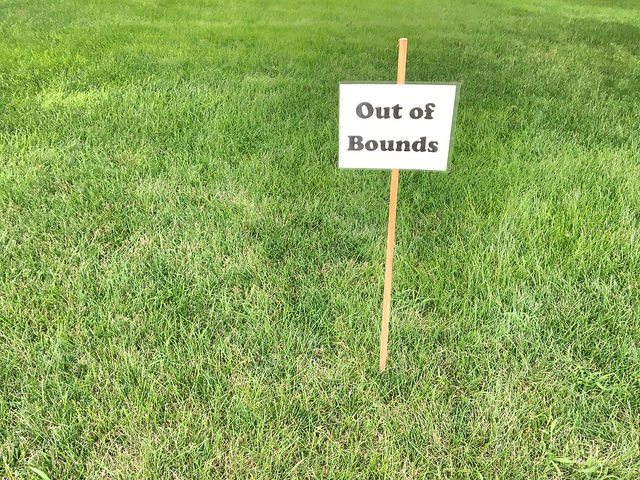
\includegraphics[width=0.6\textwidth]{images/bounds.jpg}\\
		\hspace*{15pt}\hbox{\scriptsize Image By:\thinspace{\itshape David Mulder}}
		%https://www.flickr.com/photos/113026679@N03/43459273171
	\end{center}
\end{frame}

\begin{frame}
	\frametitle{A lower bound}
	\framesubtitle{Omega}
	\begin{definition}[Big-$\Omega$ (Omega)]
		A function $f(n)$ is $\Omega(g(n))$ iff there is a positive real constant $c$ and a positive integer $n_0$ such that for
		all $n \geq n_0$ it holds that $f(n) \geq c g(n)$. In other words:\\
		$\exists c \in \mathbb{R}, \exists n_0 \in \mathbb{N} (c > 0 \wedge n_0 \geq 1 \wedge (\forall n \in \mathbb{N} (n
		\geq n_0 \to f(n) \geq cg(n))))$.
	\end{definition}
	
	\begin{block}{What of it?}
		Assume that $f(n)$ is $O(g(n))$ what, if anything, can we now conclude?
		\begin{enumerate}[A.]
			\item $f(n)$ is $\Omega(g(n))$
			\item $g(n)$ is $O(f(n))$
			\item $g(n)$ is $\Omega(f(n))$
			\item None of the above.
			\item I don't know.
		\end{enumerate}
	\end{block}
\end{frame}

\begin{frame}
	\frametitle{So what?}
	\begin{block}{Why do we care?}
		What can we use big-$\Omega$ for?
	\end{block}
	
	\begin{block}{Not much!}
		Very very little :) \\
		
		Though occassionally we can prove things require e.g.\ $\Omega(n)$ steps, even if we do not know how to solve it
		exactly.\\
		
		But if something is both $O(f(n))$ and $\Omega(f(n))$\dots
	\end{block}
	
	\begin{definition}[Big-$\Theta$ (Theta)]
		A function $f(n)$ is $\Theta(g(n))$ iff there are positive real constants $c_0, c_1$ and a positive integer $n_0$ such that for
		all $n \geq n_0$ it holds that $c_0 g(n) \leq f(n) \leq c_1 g(n)$. In other words:\\
		{\small
		$\exists c_0,c_1 \in \mathbb{R}, \exists n_0 \in \mathbb{N} (c_0> 0 \wedge c_1 > 0\wedge n_0 \geq 1 \wedge (\forall
		n \in \mathbb{N} (n \geq n_0 \to c_1 g(n) \leq f(n) \leq c_2 g(n))))$.
	}
	\end{definition}
\end{frame}

\begin{frame}
	\vspace{-10pt}
	\begin{overlayarea}{\textwidth}{\textheight}
			\begin{block}{Why do we care about this?}
				So is big-$\Theta$ any use?
			\end{block}
			
	\vspace{-5pt}
			\begin{block}{Yes!}
				It is basically the ``tight upper bound'' we discussed yesterday.
			\end{block}
			
	\vspace{-5pt}
		\only<-5>{
			\begin{columns}
				\column{0.455\textwidth}
				\lstinputlisting{src/big-oh-example.py}
					
				\column{0.455\textwidth}
				\alt<5>{
					\begin{block}{Run time}
						The run time is described as $T(n) = c_0 + c_1n + c_2n^2$, where
						\begin{itemize}
							\item $c_0$ is for lines 2, 5, and 9.
							\item $c_1n$ is for the range in line 3.
							\item $c_2n^2$ is for lines 4, 5, and 8.
						\end{itemize}
						Thus $T(n)$ is $\Theta(n^2)$.
					\end{block}
					}{
					\begin{block}{So\dots}
						What is a tight bound on the run time of \texttt{maya}?
						\begin{enumerate}[A.]
						\small
							\item $\Theta(1)$
							\item $\Theta(n)$
							\item $\Theta(n^2)$
							\item $\Theta(n^3)$
							\item I don't know.
						\end{enumerate}
					\end{block}
				}
			\end{columns}
		}
		\only<6>{
				\begin{alertblock}{Despite all that...}
					We still often \textit{just} ask for ``a tight upper bound'' and will accept a big-Oh.
				\end{alertblock}	
		}
	\end{overlayarea}
\end{frame}


% \section[Sys]{System Design}

	% %%%%%%%%%%%%%%%%%%%%%%%%%%%%%%%%%%%%%%%%%%%%%%%%%%%%%%%%%%%%%%%%%%%%%%
\begin{frame}[fragile]\frametitle{}
\begin{center}
{\Large System Design Concepts}
\end{center}

\end{frame}


%%%%%%%%%%%%%%%%%%%%%%%%%%%%%%%%%%%%%%%%%%%%%%%%%%%%%%%%%%%
 \begin{frame}[fragile]\frametitle{Are you?}

\begin{center}
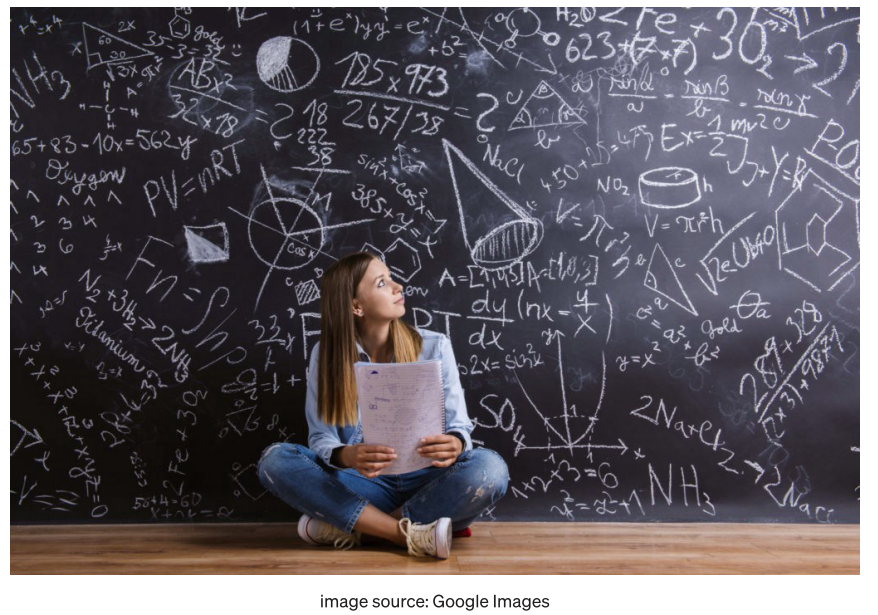
\includegraphics[width=0.8\linewidth,keepaspectratio]{qmaths}
\end{center}

\tiny{(Ref: Beginner’s Guide to Quantum Computing Literature \& Notation - Abby Mitchell)}

\end{frame}


	% %%%%%%%%%%%%%%%%%%%%%%%%%%%%%%%%%%%%%%%%%%%%%%%%%%%%%%%%%%%%%%%%%%%%%%
\begin{frame}[fragile]\frametitle{}
\begin{center}
{\Large System Design Examples}
\end{center}

\end{frame}


%%%%%%%%%%%%%%%%%%%%%%%%%%%%%%%%%%%%%%%%%%%%%%%%%%%%%%%%%%%%%%%%%%%%%%
\begin{frame}
	\frametitle{Design a pub-sub system without persistence }
		
			\begin{itemize}
				\item 
			\end{itemize}
\end{frame}

%%%%%%%%%%%%%%%%%%%%%%%%%%%%%%%%%%%%%%%%%%%%%%%%%%%%%%%%%%%%%%%%%%%%%%
\begin{frame}
	\frametitle{Design a URL shortener }
		
			\begin{itemize}
				\item 
			\end{itemize}
\end{frame}

%%%%%%%%%%%%%%%%%%%%%%%%%%%%%%%%%%%%%%%%%%%%%%%%%%%%%%%%%%%%%%%%%%%%%%
\begin{frame}
	\frametitle{Design a email/messaging system}
		
			\begin{itemize}
				\item 
			\end{itemize}
\end{frame}

%%%%%%%%%%%%%%%%%%%%%%%%%%%%%%%%%%%%%%%%%%%%%%%%%%%%%%%%%%%%%%%%%%%%%%
\begin{frame}
	\frametitle{Design Quora feed page }
		
			\begin{itemize}
				\item 
			\end{itemize}
\end{frame}

%%%%%%%%%%%%%%%%%%%%%%%%%%%%%%%%%%%%%%%%%%%%%%%%%%%%%%%%%%%%%%%%%%%%%%
\begin{frame}
	\frametitle{Design a system for processing jobs}
		
			\begin{itemize}
				\item 
			\end{itemize}
\end{frame}

%%%%%%%%%%%%%%%%%%%%%%%%%%%%%%%%%%%%%%%%%%%%%%%%%%%%%%%%%%%%%%%%%%%%%%
\begin{frame}
	\frametitle{Design a Youtube clone}
		
			\begin{itemize}
				\item 
			\end{itemize}
\end{frame}

%%%%%%%%%%%%%%%%%%%%%%%%%%%%%%%%%%%%%%%%%%%%%%%%%%%%%%%%%%%%%%%%%%%%%%
\begin{frame}
	\frametitle{Design a Json Parser }
		
			\begin{itemize}
				\item 
			\end{itemize}
\end{frame}

%%%%%%%%%%%%%%%%%%%%%%%%%%%%%%%%%%%%%%%%%%%%%%%%%%%%%%%%%%%%%%%%%%%%%%
\begin{frame}
	\frametitle{Design a data pipeline for a Machine Learning system}
		
			\begin{itemize}
				\item 
			\end{itemize}
\end{frame}

%%%%%%%%%%%%%%%%%%%%%%%%%%%%%%%%%%%%%%%%%%%%%%%%%%%%%%%%%%%%%%%%%%%%%%
\begin{frame}
	\frametitle{Design a multi-level cache }
		
			\begin{itemize}
				\item 
			\end{itemize}
\end{frame}


% \section[Probs]{Problem Solving}
	% %%%%%%%%%%%%%%%%%%%%%%%%%%%%%%%%%%%%%%%%%%%%%%%%%%%%%%%%%%%%%%%%%%%%%%
\begin{frame}[fragile]\frametitle{}
\begin{center}
{\Large Problems and Solutions from LeetCode}
\end{center}

	{\tiny (Ref :  https://www.youtube.com/watch?v=sUicrnHwA0s\&list=PLiC1doDIe9rDFw1v-pPMBYvD6k1ZotNRO)}

\end{frame}

%%%%%%%%%%%%%%%%%%%%%%%%%%%%%%%%%%%%%%%%%%%%%%%%%%%%%%%%%%%%%%%%%%%%%%
\begin{frame}[fragile]\frametitle{1. Two Sum}

	\begin{itemize}
	\item Given an array of integers, return indices of the two numbers such that they add up to a specific target
	\item \lstinline|nums =  [2,7,11,15], target = 9, as nums[0] + nums[1] = 2 + 7 = 9, return [0,1]|
	\end{itemize}
	
	\begin{columns}[T]
		\column{0.455\linewidth}
		\begin{lstlisting}[basicstyle=\scriptsize]
# Brute force ie two for loops, so O(n^2)
def two_sum_brute(nums, target):
		for i in range(len(nums) - 1):
				for j in range(i + 1, len(nums)):
						if nums[i] + nums[j] == target:
								return [i, j]
		return [-1, -1]		
		\end{lstlisting}
		\column{0.455\linewidth}
		\begin{lstlisting}[basicstyle=\scriptsize]
# Loop once, dictionary based, so O(n)
def two_sum_dict(nums, target):
		seen = {}
		for i, num in enumerate(nums):
				if target - num in seen:
						return [seen[target - num], i]
				elif num not in seen:
						seen[num] = i
		return [-1, -1]	
				\end{lstlisting}		
	\end{columns}
	
	
\end{frame}


%%%%%%%%%%%%%%%%%%%%%%%%%%%%%%%%%%%%%%%%%%%%%%%%%%%%%%%%%%%%%%%%%%%%%%
\begin{frame}[fragile]\frametitle{2. Add Two Numbers}


	\begin{itemize}
	\item Given two linked lists representing 2 numbers, digits are stored in reverse order. Add both and return result as list
	\item \lstinline|(2->4->3) + (5->6->4), so numbers are 342 + 465 = 807, so result is (7->0->8)|
	\end{itemize}
	
	\begin{columns}[T]
		\column{0.455\linewidth}
		\begin{lstlisting}[basicstyle=\scriptsize]
# Definition of singly-linked list
class ListNode:
    def __init__(self, val=0, next=None):
        self.val = val
        self.next = next
				
# position wise addition, and carry forward
def addTwoNumbers(l1, l2):
    added = ListNode(val=(l1.val + l2.val) % 10)
    carry_over = (l1.val + l2.val) // 10
    current_node = added
    while (l1.next and l2.next):
        l1 = l1.next
        l2 = l2.next
				current_sum = carry_over + l1.val + l2.val
        current_node.next = ListNode(val=current_sum % 10)
        carry_over = current_sum // 10
        current_node = current_node.next				
		\end{lstlisting}
		\column{0.455\linewidth}
		\begin{lstlisting}[basicstyle=\scriptsize]
    while(l1.next):
        l1 = l1.next
				current_sum = carry_over + l1.val 
        current_node.next = ListNode(val=current_sum % 10)
        carry_over = current_sum // 10
        current_node = current_node.next

    while(l2.next):
        l2 = l2.next
				current_sum = carry_over + l2.val
        current_node.next = ListNode(val=current_sum % 10)
        carry_over = current_sum // 10
        current_node = current_node.next

    if carry_over > 0:
        current_node.next = ListNode(val=1)
    return added
				\end{lstlisting}		
	\end{columns}
	
\end{frame}

%%%%%%%%%%%%%%%%%%%%%%%%%%%%%%%%%%%%%%%%%%%%%%%%%%%%%%%%%%%%%%%%%%%%%%
\begin{frame}[fragile]\frametitle{3. Longest Substring without repeating characters}


	\begin{itemize}
	\item Given a string find the length of the longest substring without repeating characters
	\item \lstinline|"abcabcbb" => 3 for "abc" ; "bbbbbbbbbb" => 1 for "b"|
	\end{itemize}
	
	\begin{columns}[T]
		\column{0.5\linewidth}
	\begin{itemize}
	\item Go on string letters one by one, store each with its index, till you find a duplicate 
	\item In ``abcabcbb'' you will go till 2nd `a', storing \lstinline|{'a'=0,'b'=1,'c'=2}| 
	\item Once duplicate is found, within the same substring, reset start of the next search at letter next to first duplicates ie 2nd 'b'
	\item Capture current substring length as current index which is 3 - index of the first conflict letter, ie 0, so length = 3
	\item Start search similarly from 2nd 'b'
	\end{itemize}
		\column{0.455\linewidth}
		\begin{lstlisting}[basicstyle=\scriptsize]
def lengthOfLongestSubstring(s):
    substring = dict()
    current_substring_start = 0
    current_substring_length = 0
    longest_substring_sofar = 0
    for i, letter in enumerate(s):
        if letter in substring and substring[letter] >= current_substring_start:
            current_substring_start = substring[letter] + 1
            current_substring_length = i - substring[letter]
            substring[letter] = i
        else:
            substring[letter] = i
            current_substring_length += 1
            if current_substring_length > longest_substring_sofar:
                longest_substring_sofar = current_substring_length
    return longest_substring_sofar
				\end{lstlisting}		
	\end{columns}
	
\end{frame}

%%%%%%%%%%%%%%%%%%%%%%%%%%%%%%%%%%%%%%%%%%%%%%%%%%%%%%%%%%%%%%%%%%%%%%
\begin{frame}[fragile]\frametitle{5. Longest Palindromic Substring}


	\begin{itemize}
	\item Given a string s, return longest palindromic substring in s
	\item \lstinline|"babad" => "bab", "aba"|
	\item Brute Force: e.g. ``abcbd''. Brute force could be to run 2 for loops, for different ranges, longest to shortest and check for palindrome, return first hit of the longest
	\item Better to find centers having palindrome around it, by expanding step by step. Store biggest so far. Take care of Odd and Even lengths. Find lengthier than current biggest.
	\end{itemize}
	


		\begin{lstlisting}[basicstyle=\scriptsize]
def is_palindrome(s):
    return s == s[::-1]
		
def longestPalindromicSubstring_bruteforce(s):
    for length in range(len(s), 0, -1):  # reverse length numbers
        for start_index in range(0, len(s) + 1 - length):  # different starting points
            current_substring = s[start_index:(start_index + length)]
            if is_palindrome(current_substring):
                return current_substring  # return right away because we are checking the longest first
		\end{lstlisting}		


\end{frame}

%%%%%%%%%%%%%%%%%%%%%%%%%%%%%%%%%%%%%%%%%%%%%%%%%%%%%%%%%%%%%%%%%%%%%%
\begin{frame}[fragile]\frametitle{5. Longest Palindromic Substring}

		\begin{lstlisting}[basicstyle=\scriptsize]
def longestPalindromicSubstring(s):
    biggest = s[0]
    step = len(biggest) // 2  # one side
    # odd case
    for center in range(1, len(s) - 1):
        bounds = [center - (1 + step), center + (1 + step)]  # both directions
        while (bounds[0] > -1) and (bounds[1] < len(s)):  # ends
            current_string = s[bounds[0]:bounds[1] + 1]
            if is_palindrome(current_string):
                biggest = current_string
                step = len(biggest) // 2  # find longer next
                bounds[0] -= 1  # make wider
                bounds[1] += 1
            else:
                break
    # even case
    for center in range(step, len(s) - step - 1):
        bounds = [center - step, center + (1 + step)]  # both directions
        while (bounds[0] > -1) and (bounds[1] < len(s)):  # ends
            current_string = s[bounds[0]:bounds[1] + 1]
            if is_palindrome(current_string):
                biggest = current_string
                step = len(biggest) // 2  # find longer next
                bounds[0] -= 1  # make wider
                bounds[1] += 1
            else:
                break
    return biggest
		\end{lstlisting}		

\end{frame}

%%%%%%%%%%%%%%%%%%%%%%%%%%%%%%%%%%%%%%%%%%%%%%%%%%%%%%%%%%%%%%%%%%%%%%
\begin{frame}[fragile]\frametitle{6. ZigZag Conversion}


	\begin{itemize}
	\item Write code that will take a string and make zig zag on given number of rows
\lstinline{"Paypal is hiring" ie "PAYPALISHIRING" => |/|/| like order}
	\item Output : ``PAHNAPLSIIGYIR''
	\item Dictionary based solution, each key is for a row value is list of letters in it.
	\item Go on increasing row counter till num, then decreasing till 1 and so on.
	\end{itemize}

		\begin{lstlisting}[basicstyle=\scriptsize]
def convert_zigzag(s, num):
    if num == 1:
        return s
    rows_dict = {row: "" for row in range(1, num + 1)}
    current_row_index = 1
    increment_row_index = True # False for down
    for c in s: # each letter:
        rows_dict[current_row_index] += c
        if (current_row_index == 1) or ((current_row_index < num) and increment_row_index):
            current_row_index += 1
            increment_row_index = True
        else:
            current_row_index -= 1
            increment_row_index = False
    converted_string = ""
    for row in range(1, num+1):
        converted_string += rows_dict[row]
    return converted_string		
				\end{lstlisting}		

	
\end{frame}

%%%%%%%%%%%%%%%%%%%%%%%%%%%%%%%%%%%%%%%%%%%%%%%%%%%%%%%%%%%%%%%%%%%%%%
\begin{frame}[fragile]\frametitle{9. Palindrome Number}


	\begin{itemize}
	\item Determine if given integer is palindrome, without converting integer to string. Example121 is, -121 is not
	\item Conversion solution : \lstinline{return (str(x) == str(x)[::-1])}
	\item If number is negative, return False directly, as "-" can not be on right end.
	\item Separate out digits then reverse, and check with original by equality
	\end{itemize}

		\begin{lstlisting}[basicstyle=\scriptsize]
def is_palindrome(x):
    if x < 0:
        return False
    reversed_num = 0
    decimal_step = 0
    while (x // (10 ** decimal_step) !=0):
        reversed_num = (reversed_num * 10) + (x // (10 ** decimal_step) % 10)
        decimal_step += 1

    return (x == reversed_num)
				\end{lstlisting}		

	
\end{frame}

%%%%%%%%%%%%%%%%%%%%%%%%%%%%%%%%%%%%%%%%%%%%%%%%%%%%%%%%%%%%%%%%%%%%%%
\begin{frame}[fragile]\frametitle{11. Container With Most Water}


	\begin{itemize}
	\item Build histogram of numbers. With two bars as sides, find which container has most water
	\item For \lstinline{ [1,8,6,2,5,4,8,3,7] = 49}, between first and last
	\item Height as well as wider separation is needed.
	\item Brute force will be to try all pairs and finding max.
	\item Start from both ends and move in from shorter side and check.
	\end{itemize}

		\begin{lstlisting}[basicstyle=\scriptsize]
def maxArea(height):
    start_index = 0
    end_index = len(height) - 1
    largest = 0
    while start_index != end_index:
        next_area = min(height[start_index],height[end_index]) * (end_index - start_index)
        if next_area > largest:
            largest = next_area
        if height[start_index] < height[end_index]:
            start_index += 1
        else:
            end_index -= 1
    return largest
				\end{lstlisting}		

	
\end{frame}




% \section[Refs]{References}
	% \begin{frame}\frametitle{References}
Many publicly available resources have been refereed for making this presentation. Some of the notable ones are:
\footnotesize
\begin{itemize}
\item {\bf Textbook: }
{\em Data Structures and Algorithm Analysis, 2nd edition} by Mark Allen Weiss,
The Benjamin/Cummings Publishing Company, Inc.
1995. 
\item TU Delft https://gitlab.ewi.tudelft.nl/ads-maths/course-material 
\item The Complete Data Structures and Algorithms Course in Python - Udemy
\end{itemize}
\end{frame}




	\begin{frame}[c]{}
	Thanks ...
	\vspace{5mm}
	yogeshkulkarni@yahoo.com
	\end{frame}

\end{document}

